\documentclass[a4paper,10pt,twoside,openright]{book}

% Title page and headers, general formatting and options
% % % % % % % % % % % % % % % % % % % % %
% Saarland Ph.D. thesis template		%
% created by Annemarie Friedrich		%
% % % % % % % % % % % % % % % % % % % % %

% % % % % % % % % % % % % % % % % % %
% Language stuff					%
% % % % % % % % % % % % % % % % % % %

% this was for pdflatex
\usepackage[utf8]{inputenc}
\usepackage[T1]{fontenc} % adding this makes sf font look weird??
\usepackage[scaled=0.9]{helvet}

%Xelatex
% \usepackage{fontspec}
\usepackage[english]{babel}

% \setmainfont[Ligatures=TeX]{Minion Pro}
% \setmonofont{Inconsolata}
% \setsansfont{calibri}



% % % % % % % % % % % % % % % % % % %
% Layout and fonts					%
% % % % % % % % % % % % % % % % % % %

\usepackage{fancyhdr}
\usepackage{graphicx}

% layout for floats
\usepackage{float}
\usepackage{placeins}


\setlength{\parindent}{0pt}
% spacing between lines
\linespread{1.1}
\setlength{\parskip}{0.4ex plus 0.3ex minus 0.1ex}
% have nice hanging captions for figures etc.
\usepackage[labelfont=bf,format=hang]{caption}
% this needs to be before fancy header
\usepackage[includeheadfoot,a4paper,total={6in,
  9.8in},footskip=0pt,top=1in,bottom=1in,left=1in,
right=1in, bindingoffset=0.25in, heightrounded]{geometry}

%%%%%%%%%%%%%%%%%%%%%%%%%%%%%%
%% fancy header			    %%
%%%%%%%%%%%%%%%%%%%%%%%%%%%%%%

\pagestyle{fancyplain}
\renewcommand{\chaptermark}[1]{%
	\markboth{\thechapter.\ #1}{}}
\lhead[\fancyplain{}{\thepage}]%
{\fancyplain{}{\bfseries \sffamily \nouppercase \leftmark}}
\rhead[\fancyplain{}{\bfseries \sffamily \nouppercase \leftmark}]%
{\fancyplain{}{\thepage}}
\cfoot{} % no page number at bottom


%%%%%%%%%%%%%%%%%%
%%  title page  %%
%%%%%%%%%%%%%%%%%%

% Adapted from a template by Robert Dahlke and Sigmund Stintzing (LMI München 2002)
%\usepackage{german}

\newcommand{\ThesisTitle}[8]{
  \thispagestyle{empty}
  \vspace*{\stretch{1}}
  {\parindent0cm
  \rule{\linewidth}{.7ex}}
  \begin{flushright}
    \vspace*{\stretch{1}}
    \sffamily\bfseries\Huge
    #1\\
    \vspace*{\stretch{2}}
    \sffamily\bfseries\large
    #2
    \vspace*{\stretch{1}}
  \end{flushright}
  \rule{\linewidth}{.7ex}
  
  \vspace*{1cm}
  
  \begin{center}
	    
\includegraphics[width=1.5in]{owl}
  \end{center}

  \vspace*{\stretch{1}}
  \begin{center}
    \Large A dissertation submitted towards the degree\\
    \Large Doctor of Engineering\\
    \Large of the Faculty of Mathematics and Computer Science\\
    \Large of Saarland University\\
     \vspace*{0.5cm}
    \large by\\
    \large #2\\
    \vspace*{0.5cm}
    \large  \sffamily Saarbr\"ucken, den #3
  \end{center}

  \newpage
  \thispagestyle{empty}

  \vspace*{\stretch{1}}

  \begin{flushleft}
  	\large Dekan: #4 \\[1mm]
    \large Erstgutachter:  #5 \\[1mm]
    \large Zweitgutachter: #6 \\[1mm]
    \large Drittgutachter: #7 \\[1mm]
    \large Tag der m\"undlichen Pr\"ufung: #8\\
  \end{flushleft}

  \cleardoublepage
}


% % % % Chapter headings % % % % %
\usepackage[raggedright]{titlesec}

% fixes a bug in current texlive installation
% http://tex.stackexchange.com/questions/299969/titlesec-loss-of-section-numbering-with-the-new-update-2016-03-15
\usepackage{etoolbox}
\makeatletter
\patchcmd{\ttlh@hang}{\parindent\z@}{\parindent\z@\leavevmode}{}{}
\patchcmd{\ttlh@hang}{\noindent}{}{}{}
\makeatother

\titleformat{\chapter}[display]
{\normalfont\sffamily\LARGE\bfseries}
{\chaptertitlename\ \thechapter}{0pt}{\rmfamily\Huge\rule{\linewidth}{.2ex}\raggedright\\}[\vspace*{-0.6cm}\rule{\linewidth}{.2ex}]

\titleformat{\part}[display]
{\normalfont\sffamily\Huge\bfseries\centering}
{\partname\ \thepart\\ \rule{\linewidth}{.3ex}}{10pt}{}
 




% % % % % % % % % % % % % % % % % % %
% citation							%
% % % % % % % % % % % % % % % % % % %
\usepackage[numbers,sort&compress]{natbib}
\usepackage[toc,page]{appendix}
\usepackage{bibentry}
\nobibliography*

% \bibliographystyle{plainnat}


\usepackage{amsmath}
\usepackage{listings}
\lstset{
  numbers=left,
  numbersep=10pt,
  numberstyle=\tiny\color{gray},
  basicstyle=\ttfamily\small,
  escapeinside={@}{@},
  keywordstyle=\ttfamily,
  firstnumber=1,
  showspaces=false,
  numberfirstline=true,
  columns=fullflexible,
  captionpos=b,
  % language=Pascal,
  mathescape=true,
  xleftmargin=0.7in
}


\captionsetup{justification=centering}


\usepackage{tikz}
\usepackage{amsthm}
\usepackage{lmodern}%[lighttt]
\usepackage[utf8]{inputenc}
\usepackage[T1]{fontenc}
\usepackage{amssymb}

\usepackage{hyperref}


%\usepackage{semantic}
\usepackage{mathpartir}

\usepackage{xspace}
\usepackage{fixltx2e}
\usepackage{framed}
\usepackage{relsize}


% % % % % % % % % % % % % % % % % % %
% graphics etc						%
% % % % % % % % % % % % % % % % % % %
\usepackage{graphicx}
% \usepackage[usenames,dvipsnames]{xcolor}
% todonotes: useful while writing!
\usepackage[backgroundcolor=yellow!30]{todonotes}
% for showing todonotes properly
\setlength{\marginparwidth}{2.2cm}
%\reversemarginpar

% % % % % % % % % % % % % % % % % % %
% useful custom commands			%
% % % % % % % % % % % % % % % % % % %

% dense underline
\newcommand{\dul}[1]{\underline{\smash{#1}}}


% % % % % % % % % % % % % % % % % % %
% stuff to create nice tables		%
% % % % % % % % % % % % % % % % % % %
\usepackage{booktabs} % For \toprule, \midrule and \bottomrule
\usepackage{siunitx} % Formats the units and values
%\usepackage{pgfplotstable} % Generates table from .csv
\usepackage{multirow}
\usepackage{longtable} % for tables breaking pages
\usepackage{array}
\usepackage{dcolumn}
%here we're setting up a version of the math fonts with normal x-width
\DeclareMathVersion{nxbold}
\SetSymbolFont{operators}{nxbold}{OT1}{cmr} {b}{n}
\SetSymbolFont{letters}  {nxbold}{OML}{cmm} {b}{it}
\SetSymbolFont{symbols}  {nxbold}{OMS}{cmsy}{b}{n}

%\usepackage{arydshln} % dashed lines
\usepackage{ragged2e}
\newcolumntype{P}[1]{>{\RaggedRight\hspace{0pt}}p{#1}}
\usepackage{adjustbox}
\usepackage{tabularx}
\newcolumntype{R}[2]{%
	>{\adjustbox{angle=#1,lap=\width-(#2)}\bgroup}%
	l%
	<{\egroup}%
}
\newcommand*\rot{\multicolumn{1}{R{45}{1em}}}% no optional argument here, please!
\newcommand*\rotVert{\multicolumn{1}{R{90}{1em}|}}% no optional argument here, please!


% % % % % % % % % % % % % % % % % % %
% environments						%
% % % % % % % % % % % % % % % % % % %
\usepackage{url}
\usepackage{indent}
\usepackage{textcomp}
\usepackage{enumerate}
\usepackage{verbatim} % for comments
\usepackage{fancyvrb}
\usepackage{listings} % for comments
\usepackage{qtree} % for syntactic trees (images)
\usepackage{booktabs} % for nice tables
\usepackage{colortbl}


\newenvironment{packed_enum}{
	\begin{enumerate}
		\setlength{\itemsep}{1pt}
		\setlength{\parskip}{0pt}
		\setlength{\parsep}{0pt}
		\setlength{\leftmargin}{0pt}
	}{\end{enumerate}}

\newenvironment{packed_enum_more_indent}{
	\begin{enumerate}
		\setlength{\itemsep}{1pt}
		\setlength{\parskip}{0pt}
		\setlength{\parsep}{0pt}
		\setlength{\leftmargin}{4pt}
	}{\end{enumerate}}

\newenvironment{packed_item}{
	\begin{itemize}
		\setlength{\itemsep}{1pt}
		\setlength{\parskip}{0pt}
		\setlength{\parsep}{0pt}
		\setlength{\leftmargin}{0pt}
	}{\end{itemize}}

\newenvironment{packed_list}{
	\begin{list}
		\setlength{\itemsep}{1pt}
		\setlength{\parskip}{0pt}
		\setlength{\parsep}{0pt}
		\setlength{\leftmargin}{0pt}
	}{\end{list}}

\setlength{\fboxsep}{0.3cm}
\setlength{\fboxrule}{1pt}

% Example environment (for language examples)
% use with \begin{example}
%... 
%\end{example}

\newcounter{examplecounter}
\newlength\myLeftmargin
\setlength{\myLeftmargin}{0pt}
\newenvironment{example}
{\refstepcounter{examplecounter}
\begin{samepage}
\begin{indentation}{2.5em}{0em} % first: indent on left side, second: indent on right side
	\setlength{\parsep}{0pt}
	\setlength{\parskip}{0pt}
	\setlength{\itemsep}{0pt}
	\begin{list}{\textbf{(\arabic{examplecounter})}}%
		{\global\addtolength\myLeftmargin{\parindent}%
			\global\addtolength\myLeftmargin{\parindent}
			\setlength\leftmargin{\myLeftmargin}%
		}
		\item\relax}
	{\end{list}
\end{indentation}
\end{samepage}
}
	
\usepackage[utf8]{inputenc}
\usepackage{amssymb}
\usepackage{amsmath}
\setcounter{tocdepth}{1}
\setcounter{secnumdepth}{3}
\usepackage{graphicx}
\usepackage{multicol}
\usepackage{color}
\usepackage{hyperref}
\usepackage{listings}
\usepackage{fancyvrb}
\usepackage{amsthm}
\usepackage{mathtools}
\usepackage{algpseudocode}
\usepackage{semantic}
\usepackage{chngcntr}
\usepackage{url}
\usepackage{paralist}
\usepackage{enumitem}
\usepackage{framed}
\usepackage{mdframed}
\usepackage{mathpartir}
\usepackage{tabularx}
\usepackage{hhline}
\usepackage{parcolumns}

\counterwithin*{paragraph}{subsection}


% reset example count in each chapter
\makeatletter
\@addtoreset{examplecounter}{chapter}
\makeatother
	
\newcommand{\labex}[1]{\label{ex:#1}}
	
% modular references
\newcommand{\eref}[2][]{(\ref{ex:#2}#1)} %examples
\newcommand{\aref}[3][]{(\ref{ex:#2}#1#3)} %examples with (a) / (b)
\newcommand{\cref}[1]{Chapter~\ref{chap:#1}} % chapters
\newcommand{\dref}[1]{Definition~\ref{def:#1}} % definitions
\newcommand{\tref}[1]{Table~\ref{tab:#1}} % tables
\newcommand{\fref}[1]{Figure~\ref{fig:#1}} % figures
\newcommand{\sref}[1]{Section~\ref{sec:#1}} %sections
\newcommand{\apref}[1]{Appendix~\ref{app:#1}} %appendix sections

\newtheorem{mydef}{Definition}
\newtheorem{myLemma}{Lemma}
\newtheorem{myThm}{Theorem}
\newtheorem{myaxiom}{Axiom}
\newtheorem{mycor}{Corollary}
\newtheorem{myprop}{Proposition}


\newcommand{\expr}{\mathit{e}} 
\newcommand{\comm}{\mathit{c}}
\newcommand{\sk}{\texttt{skip}} 
% \newcommand{\lbl}{\mathit{label}} 
\newcommand{\pc}{\mathit{pc}} 
\newcommand{\lab}{\ell}
\newcommand{\TODO}[1]{\textcolor{red}{\bf #1}}
\newcommand{\pl}{\ensuremath{{}^\star}\xspace}
\newcommand{\TT}{\texttt}

% \newcommand{\inference}[3][]{\text{\smaller #1}\inferrule{ #2}{#3}}

\newcommand{\bp}{\mathit{b}}
\newcommand{\node}{\mathit{n}}
\newcommand{\cfg}{\mathcal{G}}
\newcommand{\pathG}[2]{#1 \rightarrow_p #2}
\newcommand{\dom}[2]{#1~\texttt{pd}~#2}
\newcommand{\ndom}[2]{#1~\texttt{Npd}~#2}
\newcommand{\IPD}[1]{\mathit{IPD}(#1)}
\newcommand{\SEN}{\texttt{SEN}}

\setlength{\parindent}{1em}
\setlength{\parskip}{0.5em}
\linespread{1.3}

\newcommand {\mV} {\mathcal{V}}
\newcommand {\mL} {\mathcal{L}}
\newcommand {\mH} {\mathcal{H}}
\newcommand {\mE} {\mathcal{E}}

\newcommand {\cstack} {\kappa}
\newcommand {\inst} {\iota}
\newcommand {\Succ} {\mathit{Succ}}
\newcommand {\Left} {\mathit{Left}}
\newcommand {\Right} {\mathit{Right}}
\newcommand {\src} {\mathit{src}}
\newcommand {\dst} {\mathit{dst}}
\newcommand {\isIPD} {\mathit{isIPD}}
\newcommand {\ipd} {\mathit{ipd}}
\newcommand {\cf} {\mathit{CF}}
\newcommand {\cond} {\mathit{cond}}
\newcommand {\push} {\mathit{push}}
\newcommand {\false} {\mathit{false}}
\newcommand {\true} {\mathit{true}}
\newcommand {\val} {\mathit{value}}
\newcommand {\base} {\mathit{base}}
\newcommand {\Empty} {\mathit{empty}}
\newcommand {\eV} {\mathit{excValue}}
\newcommand {\SC} {\mathit{sc}}
\newcommand {\LO} {\Lambda}
\newcommand{\CFG}{\mathit{CFG}}
\newcommand{\map}{\mu}
\newcommand{\dep}{\delta}
\newcommand{\op}{\oplus}
\newcommand{\eop}{\mathit{eop}}
\newcommand{\cop}{\oplus}
\newcommand{\aop}{\odot}
\newcommand{\lbl}{\mathit{\mathcal{A}}}
\newcommand{\bool}{\mathit{\texttt{bool}}}
\newcommand{\Vars}{\mathit{\texttt{V}}}
\newcommand{\dVars}{\dep}
% \newcommand{\know}{\kappa}
\newcommand{\aks}{\mathcal{K}}
\newcommand{\fin}{\texttt{stop}}
\newcommand{\attacker}{\ell}
\newcommand{\up}{\mathit{upgradeVars}}
\newcommand{\resetBS}{\mathit{resetBS}}
\newcommand{\tb}{\mathit{tt}}
\newcommand{\ff}{\mathit{ff}}
\newcommand {\veq}{\approx^{\beta}_L}
\newcommand {\sigeq}{\simeq_\attacker}
% \newcommand {\sigeq}{\underset{\attacker}{\simeq}}
\newcommand {\teq}{\approx^{\beta}_L}
\newcommand {\req}{\cong^{\beta}_L}
\newcommand {\sceq}{\sim^{\beta}_L}
\newcommand {\lsd}{\Gamma(!\sigma(\dst))}
\newcommand{\eq}{\sim_\attacker}
% \newcommand{\eq}{\underset{\attacker}{\sim}}
\newcommand{\bits}{\mathit{b}}
\newcommand{\trace}{\tau}
\newcommand{\emptyTrace}{\epsilon}
%% \newcommand{\proj}{\vert_\attacker}
\newcommand{\proj}{{\uparrow_\attacker}}
\newcommand{\budget}{\beta}
\newcommand{\blabel}{\mathbb{B}}
\newcommand{\ilabel}{\mathbb{L}}
\newcommand{\dec}{\texttt{declassify}}
\newcommand{\domain}{\mathit{dom}}
\newcommand{\pred}{\mathit{P}}
\newcommand{\entropy}{\mathit{H}}
\newcommand{\avg}{\mathit{avg}}
\newcommand{\Reduce}{\mathbb{R}}

\newcommand{\bscmd}{\underset{\pc}{\Downarrow}}
\newcommand{\bscmdup}{\underset{\pc \sqcup \ell}{\Downarrow}}
\newcommand{\bsexp}{\Downarrow}

\newcommand{\lirsem}{{~\underset{\pc}{\Downarrow}~}}
\newcommand{\simsem}{{~\underset{\pc}{\downarrow}~}}
\newcommand{\lirsemup}{{~\underset{\pc \sqcup k}{\Downarrow}~}}
\newcommand{\simsemup}{{~\underset{\pc \sqcup k}{\downarrow}~}}

% \newcommand{\lirsem}{{~\underset{\pc}{\downdownarrows}~}}
% \newcommand{\simsem}{{~\underset{\pc}{\downarrow}~}}
% \newcommand{\lirsemup}{{~\underset{\pc \sqcup (k, \{\})}{\downdownarrows}~}}
% \newcommand{\simsemup}{{~\underset{\pc \sqcup (k, \{\})}{\downarrow}~}}

\newcommand{\refrule}[1]{\textsc{\ref{#1}}}

\newcommand{\sys}{\mbox{WebPol}}

\makeatletter % allow us to mention @-commands
\def\arcr{\@arraycr}
\makeatother

\makeatletter
\newcommand{\labelthis}[2]{%
  \def\@currentlabel{#2}\ltx@label{#1}#2%
}
\makeatother

\makeatletter
\def\blfootnote{\xdef\@thefnmark{}\@footnotetext}
\makeatother

\hyphenation{term-i-na-tion-in-sen-si-tive}

% Local Variables:
% TeX-engine: xetex
% End:



\usepackage{blindtext}
%%% TO CHANGE THE FONT - CHANGE THIS PACKAGE
\usepackage{tgpagella}
\usepackage{emptypage}
\usepackage{tikzscale}
% \usepackage{filecontents}
% \begin{filecontents}{lattice.tikz}
% \begin{tikzpicture}
% \node (H) at (0,3) {$H$};
% \node (M1) at (-1,2) {$M_1$};
% %\node (M1) at (0,2) {$M_1$};
% \node (M2) at (1,2) {$M_2$};
% \node (Lp) at (0,1) {$L'$};
% \node (L1) at (-1,1) {$L_1$};
% \node (L2) at (1,1) {$L_2$};
% \node (L) at (0,0) {$L$};
	
% \tikzstyle{every path}=[black] 
% \path		(H) edge (M1)
% 			(H) edge (M2)
% 			(M1) edge (L1)
% 			(M1) edge (Lp)
% 			(M2) edge (Lp)
% 			(M2) edge (L2)
% 			(L1) edge (L)
% 			(Lp) edge (L)
% 			(L2) edge (L);				
% \end{tikzpicture}
% \end{filecontents}

\begin{document}

\frontmatter

\ThesisTitle
    {Practical Dynamic Information Flow Control} % thesis title
    {Abhishek Bichhawat}               % name of author
    {some very lucky day in the future}                  % day of submission
    {Dekan}									% name of dean
    {first advisor}                % first reviewer
    {second reviewer}            % second reviewer
    {possibly another reviewer}						% third reviewer
    {some very lucky day in the future}                  % date of oral exam / defense




% Stuff required by Uni
\pagestyle{empty}
\section*{Abstract}

% \todo[inline]
{
Over the years, computer systems and applications have grown
significantly complex while handling a plethora of private and
sensitive user information. The complexity of these applications is
often assisted by a set of (un)intentional bugs with both malicious
and non-malicious intent leading to information leaks. Information
flow control has been studied extensively as an approach to mitigate
such information leaks. The technique works by enforcing the security
property of non-interference using a specified set of security
policies. A vast majority of existing work in this area
is based on static analyses. However, some of these applications,
especially on the Web, are developed using dynamic languages like
JavaScript that makes the static analyses techniques stale and
ineffective. As a result, there has been a growing interest in recent
years to develop dynamic information flow analysis techniques. In
spite of that, dynamic information flow analysis has not been at the
helm of information flow security in settings like the Web; the prime
reason being that the analysis techniques and the security property
related to them (non-interference) either over-approximate or are too
restrictive in most cases. Concretely, the analysis techniques
generate a lot of false positives, do not allow legitimate release of
sensitive information, support only static and rigid security
policies or are not general enough to be applied to real-world
applications. 

This thesis focuses on improving the usability of dynamic information
flow techniques by presenting mechanisms that can enhance the
precision and permissiveness of the analyses. It begins by presenting
a sound improvement and enhancement of the permissive-upgrade
strategy (a strategy widely used to enforce dynamic information flow
control), which improves the strategy's permissiveness and makes it
generic in applicability. The thesis, then, presents a sound and
precise dynamic information flow analysis for handling complex
features like unstructured control flow and exceptions in higher-order 
languages. Although non-interference is a desired property for
enforcing information flow control, there are program instances that
require legitimate release of some parts of the secret data to provide
the required functionality. Towards this end, this thesis develops a sound 
approach to quantify information leaks dynamically while allowing 
information release in accordance to a pre-specified budget. The thesis
concludes by applying these techniques to an information flow
control-enabled Web browser and explores a policy specification 
mechanism that allows flexible and useful information flow policies to 
be specified for Web applications. 

}

\clearpage
\section*{Kurzzusammenfassung}

Seit Jahren werden Computersysteme und -Anwendungen immer komplexer
und verarbeiten eine Unmenge private und sensible Daten. Die
Komplexit\"at der Anwendungen tr\"agt neben der Existenz von (un)gewollt
eingef\"ugten Software Fehlern zur Weitergabe dieser sensiblen
Informationen bei. Information Flow Control (IFC, zu Deutsch
Informations-Fluss-Analyse) Mechanismen sind Gegenstand intensiver
Forschung um diesem Problem entgegen zu wirken. Grunds\"atzlich basieren
diese Ans\"atze auf der Anwendung von vordefinierten Sicherheitsregeln,
die die Unbeeinflussbarkeit (engl. non-interference) garantieren. Der
\"uberwiegende Teil dieser Techniken nutzt statische Analyse zur
Erzeugung der Regeln. Dem gegen\"uber steht die Tatsache, dass
Anwendungen, insbesondere im Bereich Web-Anwendungen, in dynamischen
Sprachen wie JavaScript entwickelt werden, wodurch rein statische
Analysen unzureichend sind. Dynamische Methoden auf der anderen Seite
approximieren das Verhalten einer Anwendung und k\"onnen daher die
grundlegende non-interference nicht garantieren. Sie tendieren dazu
besonders restriktive Regeln zu erzeugen, wodurch auch der rechtm{\"a}{\ss}ige
Zugriff auf Information verweigert wird. Beide Ans\"atze sind daher
nicht zur Anwendung auf Systeme in der realen Welt geeignet.

Das Ziel dieser Arbeit besteht darin die Benutzbarkeit von dynamischen
IFC Mechanismen zu verbessern indem Techniken entwickelt werden, die
die Genauigkeit und Toleranz steigern. Die Arbeit pr\"asentiert eine
korrekte (engl. 'sound') Erweiterung der permissive-upgrade Strategie
(eine Standardstrategie f\"ur dynamische IFC), die die Toleranz der
Strategie verbessert und sie weithin anwendbar macht. Dar\"uber hinaus
pr\"asentiere ich eine neue dynamische IFC Analyse, die auch komplexe
Funktionen, wie unstruktierte Kontrollfl\"usse und Exceptions in
Hochsprachen, abbildet. Obwohl Unbeeinflussbarkeit eine w\"unschenswerte
Eigenschaft ist, gibt es Anwendungen, die rechtm{\"a}{\ss}igen Zugang zu
sensiblen Daten ben\"otigen um ihre Funktion zu erf\"ullen. Um dies zu
erm\"oglichen pr\"asentiert diese Arbeit einen Ansatz, der die ungewollte
Weitergabe von Information quantifiziert und anhand eines
vordefinierten Grenzwertes freigibt. Diese Techniken wurden in einen
Web-Browser integriert, welcher es erlaubt die Definition von
flexiblen und n\"utzlichen Informationsflussregeln f\"ur Web Anwendungen
umzusetzen. 
% \clearpage
% \section*{Ausführliche Zusammenfassung}

\todo[inline]{long summary in German, Michaela has 5.5 pages}
\clearpage
\section*{Acknowledgment}


General acknowledgment goes here...

\subsection*{Co-authoring}


\clearpage

% % % % % % % % % % % % % % % % % % % % % % % % % % % % % % % % % % % % %

\pagestyle{fancyplain} % fancy headers from here on
\tableofcontents
\markboth{Contents}{Contents}

% % % % START OF THESIS TEXT % % % % %

% start page numbering
\mainmatter\setcounter{page}{1}

\cleardoublepage
\part{Introduction and Background}
\cleardoublepage
\chapter{Introduction}

With the growth in the use of computers and the Internet for almost
every application, the amount of sensitive information that 
programs compute has also increased dramatically. For instance,
e-commerce websites have access to the personal details of a user
including her address, credit-card details etc. Similarly, a hospital
database stores sensitive and private medical data of its
patients. While the complexity  of such systems has increased
manifold in the last few decades, the privacy and confidentiality
guarantees still remain questionable~\citep{infoleaks}. Often leaks
occur either due to buggy programs or due to malicious
code. Cryptographic techniques protect data by encrypting it but many 
programs need to operate on confidential data, which requires the data 
to be available in plaintext form. % An adversary can then attempt to
% infer the confidential data by observing such operations in the
% system.
To this end, \emph{access control} techniques are widely used
for preventing leakage of confidential data. However, once the
authorized users have access to data, there is no control on how the
data can be used. The data might be input to a program that writes to
publicly-observable locations or outputs data that is accessible to
all users.  
% For instance, a system
% can restrict access of particular confidential files to a certain set
% of authorized users.

Consider the Web, for instance. Web applications rely extensively on
third-party JavaScript to provide useful libraries, page analytics,
advertisements and many other features~\cite{nick12CCS}. JavaScript
works on a mashup model, wherein the hosting page and included scripts
share the page’s state (called the DOM). Consequently, by design, all
included third-party scripts run with the same access privileges as
the hosting page. While some third-party scripts are developed by
large, well-known, trustworthy vendors, many other scripts are
developed by small, domain-specific vendors whose commercial motives
do not always align with those of the 
webpage providers and users. This leaves sensitive information such as
passwords, credit card numbers, email addresses, click histories,
cookies and location information vulnerable to inadvertent bugs and
deliberate exfiltration by third-party scripts. In many cases,
developers are fully aware that a third-party script accesses
sensitive data to provide useful functionality, but they are unaware
that the script also leaks that data on the side. In fact, this is a
widespread problem~\cite{jang10CCS}. 
%
The traditional browser security
model is based on restricting scripts’ access to data, not on tracking
how scripts use data. Existing web security standards
and web browsers address this problem unsatisfactorily, favoring
functionality over privacy. The same-origin policy implemented
in all major browsers restricts a webpage and third-party scripts
included in it to communicating with web servers from the including
webpage’s domain only. However, broad exceptions are allowed. For
instance, there is no restriction on request parameters in urls that
fetch images and, unsurprisingly, third-party scripts leak information
by encoding it in image urls. The candidate web standard Content
Security Policy~\cite{csp}, also implemented in most browsers,
allows a page to white list scripts that may be included, but places
no restriction on scripts that have been included, thus not helping
with the problem above. 
%
Quite a few \emph{fine-grained} access control
techniques have also been proposed~\cite{conscript, adjail,
  zhouESORICS11, ccs13crypton, adsafe, fbjs, caja, webjail}. 
% For example, Conscript~\cite{conscript} allows the specification of  
% fine-grained access policies on individual scripts, limiting what
% actions every script can perform. Similarly, AdJail~\cite{adjail}
% limits the execution of third-party scripts to a shadow page and
% restricts communication between the script and the host page. Zhou and
% Evans~\cite{zhouESORICS11} take a dual approach, where fine-grained
% access control rules are attached to DOM elements. The rules specify
% which scripts can and cannot access individual elements. Along similar
% lines, Dong et al.~\cite{ccs13crypton} present a technique to isolate
% sensitive data using authenticated encryption. ADsafe~\cite{adsafe}
% and FBJS~\cite{fbjs} restrict third-party code to subsets of
% JavaScript, and use static analysis to check for illegitimate
% access. Caja~\cite{caja} uses object capabilities to mediate all
% access by third-party scripts. Webjail~\cite{webjail} supports least 
% privilege integration of third-party scripts by restricting script
% access based on high-level policies specified by the
% developer.
However, all these techniques enforce only access policies
and cannot control what a script does with data it has been provided
in good faith, i.e., if a third-party script was allowed access to
some data only for local computations, the policy places no
restriction on the script for sending it on the network while
performing the computation. More broadly, no mechanism based only
on access control can solve the problem of information leakage.  

The academic community has proposed solutions based on
\emph{information flow control} (IFC), also known as mandatory access
control.
% \emph{Information flow control} (IFC) is an
% elegant solution for such problems.
It ensures the security of
confidential information even in the presence of untrusted and buggy
code. The idea is to track the flow of information through the program
and prevent any undesired flows based on a security policy. 
Research has considered static methods such as type checking and
program analysis, which verify the security policy at compile
time~\cite{denning76, denning77, myersJFlow, volpano, pottier2003,
  hunt2006:types, LBIFS, hammer09ijis}, 
dynamic methods that track information flow through program execution
at runtime~\cite{fenton, plas09, plas10, Askarov09, Sabelfeld10, SME,
  csf12, austin12POPL, jeeves, plas14, cowl},    
and hybrid approaches that combine both static and dynamic analyses to add
precision to the analysis~\cite{Nentwich07, Gurvan06, Gurvan07,
  russo10CSF, vogt07NDSS, post14, csf15Hedin} 
for handling information leaks described above. 

Dynamic analysis has the drawback of being less precise and
introducing significant performance overheads at runtime, though it
can be more permissive than static analysis methods in some
cases~\cite{russo10CSF}. Although helpful in most 
scenarios, static analyses are mostly ineffective when working with
dynamic languages like JavaScript, which is an indispensable part of
the modern Web. The dynamic nature of
JavaScript~\cite{richards11ECOOP, oopsla13} with features like dynamic
typing, \texttt{eval},  scope-chains, prototype chains etc. makes sound
static analysis difficult. Thus, recent research has focussed on
dynamic analysis for enforcing information flow control especially in
languages like JavaScript. Even though research in dynamic information
flow control has made significant inroads in the last decade, the
applicability of these techniques still remains bleak, 
\emph{permissiveness} being the major challenge to
the practicality of dynamic information flow control. 

In recent years, researchers have explored methods to quantify the
amount of  sensitive information leaked by a program as an alternative
to the qualitative notion of information flow control. The developer
determines an ``acceptable'' upper-bound on the number of bits of
sensitive information a program may leak. Programs that leak less than
this ``acceptable'' amount of information are considered secure. The
information released is generally quantified as the
knowledge gained by an adversary about the sensitive data as a result
of the information flow in the program. Specifically, the adversary
has knowledge about the possible set of initial values that can be
associated with the sensitive data. A flow in the program could reduce
the number of possibilities, thereby increasing the knowledge of the
adversary about the specific value associated with the sensitive data
in that execution of the program. This change in knowledge can be
measured as the number of bits of information of sensitive data
released to the adversary~\cite{CoverQIF}. Statically quantifying the
information leaked by a program has been well studied in the
literature and various static quantitative information flow
measures~\cite{shannon, guessing, smith2009, clarkson2009,
  csf12GLeakage} and techniques~\cite{denning82, clark, clarkson2009,
  smith2009, backes, kopf} have been proposed. However,
quantifying information leaks in a purely dynamic setting is still
largely an open problem (prior work is limited to~\cite{mccamant}) as
dynamic analysis is generally limited to the current execution of the
program in contrast to the static methods, which analyze the program
as a whole.  

% However, in highly dynamic scenarios like the web where the
% third-party code is unknown upfront, it is difficult for the developer
% to specify an appropriate policy with declassification specifications
% that caters to all possible codes. 

% \todo[inline]{Static quantification of information leaks}

\section{Contributions of the Thesis}
This thesis focuses on improving the usability of dynamic information
flow techniques by presenting mechanisms that enhance the precision
and permissiveness of the analyses. The main contributions are as
follows: 
\begin{itemize}
\item \textbf{Generalized Permissive-Upgrade.} To improve the
    permissiveness of dynamic information flow analysis, the thesis 
    presents a sound improvement and enhancement of the
    permissive-upgrade strategy (a strategy widely used to enforce
    dynamic information flow control). The development improves the
    original strategy's permissiveness and applicability by
    generalizing the approach to an arbitrary security lattice, in
    place of the two-point lattice considered in prior work. 
\item \textbf{Precise Dynamic Information Flow Control.} Most of the
  existing work in dynamic information flow control does not handle
  complex features like unstructured control flow and exceptions. The
  proposals that handle these features are too conservative and
  require additional annotations in the program. This thesis presents a
  sound and precise dynamic information flow analysis for handling
  these features without requiring any additional annotations from the
  programmer. 
\item \textbf{Bounding Information Leaks Dynamically.} Although
  non-interference is a desired property for enforcing information
  flow control, there are program instances that  require legitimate
  release of some parts of the secret data to provide the required
  functionality. Towards this end, this thesis develops a sound
  approach to quantify information leaks dynamically while allowing
  information release in accordance with a pre-specified \emph{budget}. 
\item \textbf{Application to a Web Browser.} The thesis concludes by
  applying these techniques to an information flow control-enabled Web
  browser. An information flow control system enforces security
  policies that are a collection of rules for labeling private
  information sources, generally specified by a policy component in
  the system. To complement the work on enforcement components in Web
  browsers, this thesis explores a policy specification mechanism
  to specify flexible and useful information flow policies for Web applications. 
\end{itemize}
 
% % \Blindtext
\section{Overview}
This section presents a \emph{formal} description of the
no-sensitive-upgrade check. The technical development in this thesis
is mostly based on the simple imperative language shown in
Figure~\ref{basic:syntax}. However, the key ideas are orthogonal to
the choice of language and generalize to 
other languages easily. The use of a simpler language is to simplify
non-essential technical details. The parts in this thesis that require
a more complex language define the additional features in place. 
The language's expressions include constants or values (\TT{n}),
variables ($\TT{x}$) and unspecified binary operators ($\odot$) to 
combine them. The set of variables is fixed upfront. Labels ($\lab$)
are drawn from a fixed security lattice. The lattice contains
different labels $\{L, M, H, \ldots \}$ with a partial ordering
between the elements. Join ($\sqcup$) and meet ($\sqcap$) operations
are defined as usual on the lattice. The program counter label $\pc$
is an element of the lattice.

\subsection{Basic IFC Semantics}
%%%%%%%%%%%%%%%%%%%%%%%%%%%%%%%%%%%%
\begin{figure}
\begin{align*}
\expr	=~& \TT{n}~\arrowvert~\TT{x}~\arrowvert~\expr_1 \odot \expr_2 \\
\comm	=~& \sk~\arrowvert~\TT{x} := \expr~\arrowvert 
 ~\comm_1;\comm_2~\arrowvert~\texttt{if}~\expr~\texttt{then}~\comm_1~\texttt{else}~\comm_2~\arrowvert~\texttt{while}~\expr~\texttt{do}~\comm\\
\lab          =~& L~\arrowvert~M~\arrowvert~H~\arrowvert~\ldots\\
k,l,m, \pc =~& \lab
\end{align*}
\caption{Syntax of the Language}\label{basic:syntax}
\end{figure}

%%%%%%%%%%%%%%%%%%%%%%%%%%%%%%%%%%%%

%%%%%%%%%%%%%%%%%%%%%%%%%%%%%%%%%%%%
\begin{figure*}
\begin{framed}
\begin{mathparpagebreakable}
%\onecolumn
%%%    
\textsc{Expressions:}\\
\inferrule*[left=\mbox{\labelthis{bs:exp:c}{const}}]
{ }
{\langle \sigma, \TT{n} \rangle \bsexp \TT{n}^{\perp}}
\and
\inferrule*[left=\mbox{\labelthis{bs:exp:v}{var}}]
{\TT{n}^k := \sigma(\TT{x})}
{\langle \sigma, \TT{x} \rangle \bsexp \TT{n}^k}
\and
\inferrule*[left=\mbox{\labelthis{bs:exp:o}{oper}}]
{\langle \sigma, \expr' \rangle \bsexp
  \TT{n}'^{k'} \\ \langle \sigma, \expr'' \rangle \bsexp
  \TT{n}''^{k''} \\\\ \TT{n} := \TT{n}' \odot \TT{n}'' \\ 
  k := k' \sqcup k''} 
{\langle \sigma, \expr' \odot \expr'' \rangle \bsexp \TT{n}^k}
%%%    
\\\\
\textsc{Statements:}\\
\inferrule*[left=\mbox{\labelthis{bs:cmd:sk}{skip}}]
{ }
{\langle \sigma, \sk \rangle \bscmd \sigma}
\and
%%%
\inferrule*[left=\mbox{\labelthis{bs:cmd:s}{seq}}]
{\langle \sigma, \comm_1 \rangle \bscmd \sigma'' \\ \langle \sigma'', \comm_2 \rangle \bscmd \sigma' }
{\langle \sigma, \comm_1;\comm_2 \rangle \bscmd \sigma'}
\and
%%%
\inferrule*[left=\mbox{\labelthis{bs:cmd:wf}{while-f}}]
{\langle \sigma, \expr \rangle \bsexp \texttt{false}^{\lab}}
{\langle \sigma, \texttt{while}~\expr~\texttt{do}~\comm \rangle
  \bscmd \sigma }
\and
%%%    
\inferrule*[left=\mbox{\labelthis{bs:cmd:ie}{if-else}}]
{\langle \sigma, \expr \rangle \bsexp \TT{b}^{\lab} \\ 
  i = \left\{\begin{array}{ll}
        1, & \textit{if }~  \TT{b} = \TT{true} \arcr
        2, & \textit{otherwise } \arcr
        \end{array}\right\} \\\\ \langle
  \sigma, \comm_i \rangle \bscmdup \sigma'}
{\langle \sigma, 
  \texttt{if}~\expr~\texttt{then}~\comm_1~\texttt{else}~\comm_2
  \rangle \bscmd \sigma'}
\and
% \inferrule*[left=\mbox{\labelthis{bs:cmd:iet}{if-else-t}}]
% {\langle \sigma, \expr \rangle \bsexp \texttt{true}^{\lab} \\ \langle
%   \sigma, \comm_1 \rangle \bscmdup \sigma'}
% {\langle \sigma, 
%   \texttt{if}~\expr~\texttt{then}~\comm_1~\texttt{else}~\comm_2
%   \rangle \bscmd \sigma'}
% \and
% %%%    
% \inferrule*[left=\mbox{\labelthis{bs:cmd:ief}{if-else-f}}]
% {\langle \sigma, \expr \rangle \bsexp \texttt{false}^{\lab} \\ \langle
%   \sigma, \comm_2 \rangle \bscmdup \sigma'}
% {\langle \sigma, 
%   \texttt{if}~\expr~\texttt{then}~\comm_1~\texttt{else}~\comm_2
%   \rangle \bscmd \sigma'}
% \and
%%%    
\inferrule*[left=\mbox{\labelthis{bs:cmd:wt}{while-t}}]
{\langle \sigma, \expr \rangle \bsexp \texttt{true}^{\lab} \\ \langle
  \sigma, \comm \rangle \bscmdup \sigma'' \\\\ \langle
  \sigma'', \texttt{while}~\expr~\texttt{do}~\comm \rangle
  \bscmdup \sigma' }
{\langle \sigma, \texttt{while}~\expr~\texttt{do}~\comm \rangle
  \bscmd \sigma'}
%%%    
\end{mathparpagebreakable}
\end{framed}
\caption{Semantics}\label{fig:basic-semantics}
\end{figure*}

The rules in Figure~\ref{fig:basic-semantics} define the big-step
semantics of the language, including standard taint propagation for
IFC: the evaluation relation $\langle \sigma, \expr \rangle \bsexp
\TT{n}^k$ for expressions, and the evaluation relation $\langle \sigma,
\comm \rangle \bscmd \sigma'$ for commands. Here, $\sigma$ 
denotes a store, a map from variables to labeled values of the form
$\TT{n}^k$. \TT{b} represents a Boolean constant. For now, labels $k ::=
\lab$; this is generalized later when the ``partially-leaked'' taints
are introduced in Section~\ref{sec:existing}. 

The evaluation relation for expressions evaluates an expression
$\expr$ and returns its value $n$ and label $k$. The label $k$ is the
join of labels of all variables occurring in $\expr$ (according to
$\sigma$). The relation for commands executes a command $\comm$ in the
context of a store $\sigma$, and the current program counter label
$\pc$, and yields a new store $\sigma'$.  The function
$\Gamma(\sigma(\TT{x}))$ returns the label associated with the value in \TT{x}
in store $\sigma$: If $\sigma(\TT{x}) = \TT{n}^k$, then $\Gamma(\sigma(\TT{x})) =
k$. $\bot$ denotes the least element of the lattice. % Here, $\bot = L$.

% The rules for evaluating commands are explained below. 
The rule for
sequencing $\comm_1; \comm_2$ (\refrule{bs:cmd:s}) evaluates the
command $c_1$ under store $\sigma$ and the current $\pc$ label; this
yields a new store $\sigma''$. It then evaluates the command $c_2$
under store $\sigma''$ and the same $\pc$ label, which yields the
final store $\sigma'$. 
%
The rule for \texttt{if-else} (\refrule{bs:cmd:ie}) 
% and \refrule{bs:cmd:ief}) 
evaluates the branch condition $e$ to a Boolean value \TT{b} with
label $\lab$. Based on the value of \TT{b}, one of the branches
$\comm_1$ and $\comm_2$ is executed under a $\pc$ obtained by 
joining the current $\pc$ and the label $\lab$ of \TT{b}. Similarly, the
rules for \texttt{while} (\refrule{bs:cmd:wt} and \refrule{bs:cmd:wf})
evaluate the loop condition $e$ and execute the loop command $c_1$
while $e$ evaluates to \texttt{true}. The $\pc$ for the loop is
obtained by joining the current $\pc$ and the label 
$\lab$ of the result of evaluating $e$.

%%%%%%%%%%%%%%%%%%%%%%%%%%%%%%%%%%%%
\begin{figure*}
\begin{mathparpagebreakable}
\inferrule*[left=\mbox{\labelthis{bs:cmd:an}{assn-nsu}}]
 {l = \Gamma(\sigma(\TT{x})) \\ \pc
    \sqsubseteq l \\ \langle \sigma, \expr \rangle \bsexp \TT{n}^m
    } {\langle \sigma, \TT{x} := \expr \rangle
    \bscmd \sigma[\TT{x} \mapsto \TT{n}^{(\pc \sqcup m)}]}
\end{mathparpagebreakable}
\caption{Assignment rule for NSU}
\label{fig:assn-nsu}
\end{figure*}
%%%%%%%%%%%%%%%%%%%%%%%%%%%%%%%%%%%%

The rule for assignment statements are conspicuously missing from
Figure~\ref{fig:basic-semantics} because they depend on the strategy
used to control implicit flows. 
% In the remainder of this chapter, a number of such rules are
% considered. To start, t
The rule for assignment (\refrule{bs:cmd:an}) corresponding to the NSU
check is shown in Figure~\ref{fig:assn-nsu}. The rule checks that the
label $l$ of the assigned variable \TT{x} in the initial store $\sigma$
is at least as high as $\pc$ (premise $\pc \sqsubseteq l$). If this
condition is not true, the program gets stuck. This is exactly the NSU
check described in Section~\ref{sec:bg-nsu}.

\subsection{Formalization of the No-sensitive-upgrade Check}

% Figure~\ref{fig:basic-syntax} and \ref{fig:basic-semantics}
% describes the syntax and semantics  of a standard while language
% with information flow  control. Notice the assignment rule often
% imposes some condition  on the $pc$ to prohibit low assignments
% under high context. For  instance, for the no-sensitive upgrade
% check as described earlier  the assignment rule.

% \subsection{Termination-Insensitive Non-interference}

For establishing and proving the security
property of termination-insensitive non-interference (TINI), the
observational power of the adversary needs to be defined. 
An adversary at level $\attacker$ in the lattice is allowed to view
all values that have a label less than or equal to $\attacker$. To prove
the security property of non-interference, it is enough to show that
when executing a program beginning with two different memory stores
that are \emph{observationally equivalent} to an adversary, the final
memory stores are also \emph{observationally equivalent} to the
adversary. For this, the observational equivalence of two memory
stores with respect to an adversary needs to be defined. 
Store equivalence is formalized as a relation $\eq$,
indexed by lattice elements $\attacker$, representing the adversary.

\begin{mydef}[Value equivalence]
  Two labeled values $\emph{\TT{n}}_1^k$ and $\emph{\TT{n}}_2^m$ are $\lab$-equivalent,
  written $\emph{\TT{n}}_1^k \sim_\lab \emph{\TT{n}}_2^m$, iff either:
  \begin{enumerate}
  \item $(k = m) \sqsubseteq \lab$ and $\emph{\TT{n}}_1 = \emph{\TT{n}}_2$ or
  \item $k \not\sqsubseteq \lab$ and $m \not\sqsubseteq \lab$
  \end{enumerate}
\end{mydef}

This definition states that for an adversary at security level $\lab$,
two labeled values $\TT{n}_1^k$ and $\TT{n}_2^m$ are equivalent iff either
$\lab$ can access both values and $\TT{n}_1$ and $\TT{n}_2$ are equal, or it
cannot access either value ($k \not\sqsubseteq \lab$ and $m
\not\sqsubseteq \lab$). The additional constraint $k = m$ in clause
(1) is needed to prove non-interference by induction. In the lattice
$L \sqsubset H$, two values labeled $L$ and $H$ are distinguishable
for the $L$-adversary. 

\begin{mydef}[Store equivalence]
  Two stores $\sigma_1$ and $\sigma_2$ are $\lab$-equivalent,
  written $\sigma_1 \sim_\lab \sigma_2$, iff for every variable \emph{\TT{x}},
  $\sigma_1(\emph{\TT{x}}) \sim_\lab \sigma_2(\emph{\TT{x}})$.
\end{mydef}

The following theorem states TINI for the NSU check. The theorem has
been proved for various languages in the past.

\begin{myThm}[TINI for NSU]
  With the assignment rule \refrule{bs:cmd:an} from
  Figure~\ref{fig:assn-nsu}, if 
  $~\sigma_1 \sim_\lab \sigma_2$ and $\langle \sigma_1, c \rangle
  \bscmd \sigma_1' $ and $\langle \sigma_2, c
  \rangle \bscmd \sigma_2' $, then $\sigma_1' \sim_\lab
  \sigma_2'$.
\end{myThm}
\begin{proof} Standard, see e.g.,~\cite{plas09}
\end{proof}

% Although the security lattice here is restricted to two elements $L$
% and $H$, the rules of Figures~\ref{fig:basic-semantics}
% and~\ref{fig:assn-nsu}, the definition of equivalence above and the
% theorem above (for NSU) are all general and work for arbitrary
% lattices.
  
%%%%%%%%%%%%%%%%%%%%%%%%%%%%%%%%%%%%%%%%%%%%%%%%%%%%%%%%%%%%%

%%%%%%%%%%%%%%%%%%%%%%%%%%%%%%%%%%%%%%%%%%%%%%%%%%%%%%%%%%%%%

\section{Austin and Flanagan's Permissive-Upgrade Strategy}
\label{sec:existing}

To allow a dynamic IFC analysis to accept safe executions of programs
with variable upgrades due to high $\pc$, Austin and Flanagan proposed
a less restrictive strategy called the \emph{permissive-upgrade
  strategy}~\cite{plas10}. They study this strategy for a two-point
lattice $L \sqsubset H$ and their strategy does not immediately
generalize to arbitrary security lattices. Whereas NSU stops a program  
when a variable's label is upgraded due to assignment in a high $pc$,
permissive-upgrade allows the assignment, but labels the variable as 
\emph{partially-leaked} or $P$. The exact intuition behind the
partially-leaked label $P$ is the following: 

\begin{framed}
\noindent
  A variable with a value labeled $P$ may have been implicitly
  influenced by $H$-labeled values in this execution, but in other
  executions (obtainable by changing $H$-labeled values in the
  initial store), this implicit influence may not exist and, hence,
  the variable may be labeled $L$.
\end{framed}

%  The taint $P$ roughly means that the
% variable's content in this execution is $H$, but it may be $L$ in
% other executions.
The program must be stopped later if it tries to use
or case-analyze the variable (in particular, branching on a
partially-leaked Boolean variable is stopped). Permissive-upgrade also
ensures termination-insensitive non-interference, but is strictly more
permissive than NSU. For example, permissive-upgrade stops the leaky
program of Listing~\ref{lst1} at line~\ref{linerefcond} when \TT{z}
contains $\texttt{false}^H$, but it allows the program of
Listing~\ref{lst1.1} to execute to completion when \TT{y} contains
$\texttt{true}^L$. 
% Note that in this section, the lattice has
% only two levels: $L$ (public) and $H$ (confidential). 

In the revised syntax of labels, summarized in
Figure~\ref{pus:syntax}, the labels $k,l,m$ on values can be either
elements of the lattice  ($L, H$) or $P$. The $\pc$ can only be one of
$L, H$ because branching on partially-leaked values is
prohibited. The join operation $\sqcup$ is lifted to labels including
$P$. Joining any label with $P$ results in $P$. For brevity in
definitions, they extend the order $\sqsubset$ to $L \sqsubset H
\sqsubset P$. However, $P$ is not a new ``top'' member of the lattice
because it receives special treatment in the semantic rules. 

\begin{figure}
\begin{equation*}
\begin{aligned}[c]
\lab          =~& L~\arrowvert~H\\
\pc          =~& \lab\\
k,l,m =~& \lab~\arrowvert~P
\end{aligned}
\qquad \qquad \qquad
\begin{aligned}[c] 
k \sqcup k ~= ~& k\\
L \sqcup H ~=~ &H\\
L \sqcup P  ~=~&P \\
H\sqcup P  ~=~&P
\end{aligned}
% \end{align*}
\end{equation*}
\caption{Syntax of labels including the partially-leaked label
  $P$}\label{pus:syntax}
\end{figure}


The rule for assignment with permissive-upgrade is
\begin{mathpar}
\inferrule*[left=\mbox{\labelthis{bs:cmd:ap}{assn-pus}}]
{l := \Gamma(\sigma(\TT{x})) \qquad \langle
 \sigma, \expr \rangle \bsexp \TT{n}^m} {\langle \sigma, \TT{x} := \expr
    \rangle \bscmd \sigma[\TT{x} \mapsto \TT{n}^{k}]}
\end{mathpar}
where $k$ is defined as follows:
$$ k = % \left\lbrace
\begin{cases}
m & \mbox{ if } \pc = L \\
m \sqcup H  & \mbox{ if } \pc = H \mbox{ and } l = H\\
P  & \mbox{ otherwise}
\end{cases} % \right.
$$


% The rule for assignment with permissive-upgrade is
% \begin{align*}
%   \inference[assn-PUS: ] {l := \Gamma(\sigma(x)) \qquad \langle
%     \expr, \sigma \rangle \Downarrow n^m} {\langle x := \expr, \sigma
%     \rangle \Downarrow_\pc \sigma[x \mapsto n^{k}]}
% \end{align*}
% where $k$ is defined as follows:
% \[ k = \left\lbrace
% \begin{array}{l}
% m \mbox{ if } \pc = L \\
% m \sqcup H  \mbox{ if } \pc = H \mbox{ and } l = H\\
% P \mbox{ otherwise}
% \end{array} \right.
% \]
The first two conditions in the definition of $k$ correspond to the
NSU rule (Figure~\ref{fig:assn-nsu}). The third condition applies, in
particular, when a variable whose initial label is $L$ is assigned 
with $\pc = H$. The NSU check would stop this assignment. With
permissive-upgrade, however, the updated variable is labeled $P$,
consistent with the intuitive meaning of $P$. This allows 
more permissiveness by allowing the assignment to proceed in all
cases. To compensate, any program (in particular, an adversarial
program) is disallowed from case analyzing any value labeled 
$P$. Consequently, in the rules for \texttt{if-then} and
\texttt{while} (Figure~\ref{fig:basic-semantics}), the label of the
branch condition is of the form $\lab$, which does not include $P$. 
Thus, assignments under high $\pc$ succeed under the
permissive-upgrade check but branching or case-analyzing a
partially-leaked value is not permitted as that can also leak
information. 
% To illustrate the permissivness of the permissive-upgrade
% check, consider the different executions of example in
% Listing~\ref{lst1} taken from~\cite{plas10} as shown in
% Table~\ref{tbl:nsu}. The assignment  on line~\ref{lineref} is not
% permitted by the NSU check. However, the permissive-upgrade check
% updates \TT{y} to \texttt{false} with a partially-leaked
% label. Further case analysis on \TT{y} is prohibited (if 
% not, the branch on line~\ref{linerefcond} would not be taken as \TT{y} is
% \texttt{false} and \TT{z} would return $\texttt{true}^{L}$, thus leaking
% the value of \TT{x}).

% \begin{table*}
% \centering
% \begin{tabular} {|l||@{\,}c@{\,}||@{\,}c@{\,}|@{\,}c@{\,}|}
% \hline
% &
% $\TT{x} = \texttt{false}^{H}$
% &
% \multicolumn{2}{c|}{$\TT{x} = \texttt{true}^{H}$}
% \\
% \cline{2-4}
% &
% \textit{All strategies}
% &
% \textit{NSU}
% &
% \textit{Permissive-upgrade}
% \\
% \hline
% \TT{y} = \texttt{true} &$\TT{y} = \texttt{true}^{L}$&$\TT{y} =
%                                               \texttt{true}^{L}$&$\TT{y} =
%                                                                   \texttt{true}^{L}$\\
% \TT{z} = \texttt{true} &$\TT{z} = \texttt{true}^{L}$&$\TT{z} =
%                                               \texttt{true}^{L}$&$\TT{z} =
%                                                                   \texttt{true}^{L}$\\
% \texttt{if} (\TT{x})&branch not taken&$\pc = H$&$\pc = H$\\
% \quad\TT{y} = \texttt{false}&$\TT{y} = \texttt{true}^{L}$&execution halted&$\TT{y} = \texttt{false}^{P}$\\
% \texttt{if} (\TT{y})&$\pc = L$&&execution halted\\
% \quad$\TT{z} = \texttt{false}$&$\TT{z} = \texttt{false}^{L}$&&\\
% \texttt{return} \TT{z}&$\texttt{false}^{L}$&&\\
% \hline
% Result & $\TT{z} = \texttt{false}^{L}$ & no leak & no leak\\
% \hline
% \end{tabular}
% \caption{Execution steps in two runs of the program from
%   Listing~\ref{lst1}, with NSU and the permissive-upgrade check}
% \label{tbl:nsu}
% \end{table*}


The noninterference result obtained for NSU earlier can be extended to
permissive-upgrade by changing the definition of store 
equivalence. Because no program can case-analyze a $P$-labeled value,
such a value is equivalent to any other labeled value.

\begin{mydef}
\label{def:pus}
  Two labeled values $\emph{\TT{n}}_1^k$ and $\emph{\TT{n}}_2^m$ are
  equivalent to an adversary at level $L$,
  written $\emph{\TT{n}}_1^k \sim_L \emph{\TT{n}}_2^m$, iff either:
  \begin{enumerate}
  \item $(k = m) = L$ and $\emph{\TT{n}}_1 = \emph{\TT{n}}_2$ or
  \item $k = H$ and $m = H$ or
  \item $k = P$ or $m = P$
  \end{enumerate}
\end{mydef}

\begin{mydef}
  Two stores $\sigma_1$ and $\sigma_2$ are $L$-equivalent,
  written $\sigma_1 \sim_L \sigma_2$, iff 
  $\forall \emph{\TT{x}}. \sigma_1(\emph{\TT{x}}) \sim_L \sigma_2(\emph{\TT{x}})$.
\end{mydef}

\begin{myThm}[TINI for permissive-upgrade with a two-point lattice]
  With the assignment rule \emph{assn-PUS}, if
  $~\sigma_1 \sim_L \sigma_2$ and $\langle c, \sigma_1 \rangle
  \Downarrow_\pc \sigma_1' $ and $\langle c, \sigma_2
  \rangle\Downarrow_\pc \sigma_2' $, then $\sigma_1' \sim_L
  \sigma_2'$.
\end{myThm}
\begin{proof} See~\cite{plas10}.
\end{proof}

% Note that the above definition and proof are specific to the two-point
% lattice.


% \chapter{Related Work}
\label{ch:related}

Browser security is a very widely-studied topic. Here, only closely
related work on information flow control for browsers, browser
security policies and policy enforcement techniques is described. 

\medskip\noindent\textbf{Information flow control and script
  isolation.} With the widespread use of JavaScript,
research in dynamic techniques for IFC has regained momentum.
Nonetheless, static analyses are not completely futile. Guarn\-ieri
\emph{et al.}~\cite{guarnieri11ISSTA} present a static abstract
interpretation for tracking taints in JavaScript. However, the
omnipresent \texttt{eval} construct is not supported and this approach
does not take implicit flows into account.  Chugh \emph{et al.}
propose a staged information flow approach for 
JavaScript~\cite{stagedIFC}. They perform static server-side policy
checks on statically available code and generate residual
policy-checks that are applied to dynamically loaded code.  This
approach is limited to certain JavaScript constructs excluding dynamic 
features like dynamic field access or the \texttt{with} construct.

Austin and Flanagan~\cite{plas09} propose purely dynamic IFC for
dynamically-typed languages like JavaScript. They use the
no-sensitive-upgrade (NSU) check~\cite{zdancewic02PhD} to handle
implicit flows. Their per\-mis\-sive-upgrade strategy~\cite{plas10} is
more permissive than NSU but retains ter\-mi\-na\-tion-insensitive
non-interference. This work builds on the permissive-upgrade
strategy. They also present faceted evaluation~\cite{austin12POPL},
which is the most permissive technique of the three. However, given
the performance considerations, the technique is not suitable for
enforcing information flow control in browsers.  Just
et al.~\cite{just11PLASTIC} present dynamic IFC for JavaScript
bytecode with static analysis to determine implicit flows precisely
even in the presence of semi-unstructured control flow like
\texttt{break} and \texttt{continue}. Again, NSU is leveraged to
prevent implicit flows. This thesis builds on top of their work to
enforce information flow control in browsers.

JSFlow~\cite{csf12,jsflow} is a stand-alone implementation of
a JavaScript interpreter with fine-grained taint tracking. Many
seminal ideas for labeling and tracking flows in JavaScript owe their
lineage to JSFlow, but since JSFlow is written from scratch it has
very high overheads and  introduces annotations to deal with
semi-structured control flow. It detects
security violations due to branches that have not been executed and
injects annotations to prevent these in subsequent runs. The approach
presented in this thesis relies on analyzing CFGs and does not require
annotations. To improve permissiveness,
their subsequent work~\cite{esorics12} uses testing. 

Kerschbaumer et al.~\cite{crowdflow} build an implementation of an
information flow monitor for WebKit but do not handle all implicit
flows.  A black-box approach to enforcing non-interference is based on
secure multi-execution (SME)~\cite{SME}. Bielova \emph{et
  al.}~\cite{rnib} and De Groef \emph{et al.}~\cite{flowfox} implement
SME for web browsers. These systems do not attach labels to specific
fields in the DOM. Instead, labels are attached to individual DOM
APIs.

Chudnov and Naumann~\cite{chudnov-ccs} present another approach to
fine-grained IFC for JavaScript. They rewrite source programs to add
shadow variables that hold labels and additional code that tracks
taints. This approach is inherently more portable than that of JSFlow
or the work presented in this thesis, both of which are tied to
specific, instrumented browsers. However, it is unclear how this
approach could be extended with a policy framework like {\sys} that
assigns state-dependent labels at runtime.

The work most closely related to $\sys$ is that of
Vanhoef \emph{et al.}~\cite{csf14} on stateful declassification
policies in reactive systems, including web browsers. Their policies
are similar to the ones presented here, but there are significant
differences. First, 
their policies are attached to the browser and they are managed by the
browser user rather than website developers. Second, the policies have 
coarse-granularity: They apply uniformly to all events of a certain
type. Hence, it is impossible to specify a policy that makes
keypresses in a password field secret, but makes other keypresses
public. Third, the enforcement is based on secure
multi-execution~\cite{SME}, which is, so far, not compatible with
shared state like the DOM.

COWL~\cite{cowl} enforces mandatory access control at
coarse-granularity. In COWL, third-party scripts are sandboxed. Each
script gets access to either remote servers or the host's DOM, but not
both. Scripts that need both must be re-factored to pass DOM elements
over a message-passing API (\texttt{postMessage}). This can be both
difficult and have high overhead. For scripts that do not need this
factorization, COWL is more efficient than solutions based on FGTT.

Mash-IF~\cite{mashif} uses static analysis to enforce IFC
policies. Mash-IF's model is different from {\sys}'s model. Mash-IF
policies are attached only to DOM nodes and there is no support for
adding policies to new objects or events. Also, in Mash-IF, the
browser user (not the website developer) decides what
declassifications are allowed. Mash-IF is limited to a JavaScript
subset that excludes commonly used features such as \texttt{eval} and
dynamic property access.

JSand~\cite{jsand} uses server-side changes to the host page to
introduce wrappers around sensitive objects, in the style of object
capabilities~\cite{millerphd}. These wrappers mediate every access by
third-party scripts and can enforce rich access policies. Through
secure multi-execution, coarse-grained information flow policies are
also supported. However, as mentioned earlier, it is unclear how
secure multi-execution can be used with scripts that share state with
the host page.

{\sys} policies are enforced using an underlying IFC
component. Although, in principle, any IFC technique such as
fine-grained taint tracking~\cite{jang10CCS,jsflow,post14},
coarse-grained taint tracking~\cite{cowl} or secure
multi-execution~\cite{SME} can be used with {\sys}, to leverage the
full expressiveness of {\sys}'s finely-granular policies, a
fine-grained IFC technique is needed. 

\medskip\noindent\textbf{Access control.}  The traditional browser
security model is based on restricting scripts' access to data, not on
tracking how scripts use data. In the traditional model, it is
impossible to allow scripts access to data they need for legitimate
purposes and, simultaneously, to prevent them from leaking the data on
the side, which is the goal of IFC and {\sys}. More broadly, no
mechanism based only on access control can solve this
problem. Nonetheless, some closely related work on access
control in web browsers is discussed below.

All browsers today implement the same-origin policy (SOP)~\cite{sop},
which prevents a page and scripts included in it from making requests
to domains other than the page's host. However, for pragmatic reasons,
image requests are exempt, which is sufficient to leak
information. Consequently, the SOP is not effective against malicious
or buggy scripts. Cross-origin resource sharing (CORS)~\cite{cors}
relaxes the SOP further to allow some cross-origin requests.
%
%% Besides IFC, there is a significant amount of work on \emph{access
%%   control} in web browsers. Access control either allows or denies a
%% script access to data. It is ineffective in cases where a script
%% legitimately needs access to the data, but the risk is that it may
%% leak data on the side. Consequently, access control targets a simpler
%% problem than IFC and {\sys}---that of protecting data that the script
%% does not need in the first place. Nonetheless, we compare to some
%% closely related work on access control in web browsers.
%
Content security policies (CSPs)~\cite{csp} allow white- and
black-listing scripts. Unlike {\sys}, CSPs offer no protection against
scripts that have been included by the developer without realizing
that they leak information.

Conscript~\cite{conscript} allows the specification of fine-grained
access policies on individual scripts, limiting what actions every
script can perform. Similarly, AdJail~\cite{adjail} limits the
execution of third-party scripts to a shadow page and restricts
communication between the script and the host page.

Zhou and Evans~\cite{zhouESORICS11} take a dual approach, where
fine-grained access control rules are attached to DOM elements. The
rules specify which scripts can and cannot access individual
elements. Along similar lines, Dong \emph{et al.}~\cite{ccs13crypton}
present a technique to isolate sensitive data using authenticated
encryption. Their goal is to reduce the size of the trusted computing
base.

ADsafe~\cite{adsafe} and FBJS~\cite{fbjs} restrict third-party code to
subsets of JavaScript, and use static analysis to check for
illegitimate access. Caja~\cite{caja} uses object capabilities to
mediate all access by third-party scripts. Webjail~\cite{webjail}
supports least privilege integration of third-party scripts by
restricting script access based on high-level policies specified by
the developer.

All these techniques enforce only access policies and cannot control
what a script does with data it has access to.



%% % % % % % % % % % % % % % % % % % % % % % % % % % % % % % % % % % % % %
\cleardoublepage
\part{Generalized Permissive-Upgrade Strategy}
\cleardoublepage
\chapter{Improved Permissive-Upgrade}
\label{ch:ipu}

\begin{lstlisting}[float,label=lst1.1,caption=Impermissiveness of the NSU strategy][escapechar=@]
x = false
if (not(z))
  x = true@\label{lineref1}@
if (y) f() else g()
x = false@\label{lineref2}@
\end{lstlisting}
%
The no-sensitive-upgrade (NSU) check described earlier provides the basic
foundations for sound dynamic IFC. However, terminating a program
preemptively because of the NSU check is quite restrictive in practice. For
example, consider the program of Listing~\ref{lst1.1}, where \TT{z} is
labeled $H$ and \TT{y} is labeled $L$. This program potentially upgrades
variable \TT{x} at line~\ref{lineref1} under a high $pc$, and then
executes function \texttt{f} when \TT{y} is \texttt{true} and
executes function \texttt{g} otherwise. Suppose that \texttt{f}
does not read \TT{x}. Then, for $\TT{y} \mapsto \texttt{true}^L$, this program
leaks no information, but the NSU check would terminate this program
prematurely at line~\ref{lineref1}. (Note: \texttt{g} may read \TT{x},
so \TT{x} is not a dead variable at line~\ref{lineref1}.)

To improve permissiveness, Austin and Flanagan~\cite{plas10} proposed
the permissive-upgrade strategy as a replacement for NSU. However,
that development lacks permissiveness in certain cases. 
This chapter presents the soundness results of the permissive-upgrade
strategy with the improvement for further permissiveness in place.
 % are presented here 
% (using the modified notation for the imperative language)
% and the next
% chapter builds a generalization of the permissive-upgrade strategy to
% arbitrary lattices.


\section{Overview}
This section presents a \emph{formal} description of the
no-sensitive-upgrade check. The technical development in this thesis
is mostly based on the simple imperative language shown in
Figure~\ref{basic:syntax}. However, the key ideas are orthogonal to
the choice of language and generalize to 
other languages easily. The use of a simpler language is to simplify
non-essential technical details. The parts in this thesis that require
a more complex language define the additional features in place. 
The language's expressions include constants or values (\TT{n}),
variables ($\TT{x}$) and unspecified binary operators ($\odot$) to 
combine them. The set of variables is fixed upfront. Labels ($\lab$)
are drawn from a fixed security lattice. The lattice contains
different labels $\{L, M, H, \ldots \}$ with a partial ordering
between the elements. Join ($\sqcup$) and meet ($\sqcap$) operations
are defined as usual on the lattice. The program counter label $\pc$
is an element of the lattice.

\subsection{Basic IFC Semantics}
%%%%%%%%%%%%%%%%%%%%%%%%%%%%%%%%%%%%
\begin{figure}
\begin{align*}
\expr	=~& \TT{n}~\arrowvert~\TT{x}~\arrowvert~\expr_1 \odot \expr_2 \\
\comm	=~& \sk~\arrowvert~\TT{x} := \expr~\arrowvert 
 ~\comm_1;\comm_2~\arrowvert~\texttt{if}~\expr~\texttt{then}~\comm_1~\texttt{else}~\comm_2~\arrowvert~\texttt{while}~\expr~\texttt{do}~\comm\\
\lab          =~& L~\arrowvert~M~\arrowvert~H~\arrowvert~\ldots\\
k,l,m, \pc =~& \lab
\end{align*}
\caption{Syntax of the Language}\label{basic:syntax}
\end{figure}

%%%%%%%%%%%%%%%%%%%%%%%%%%%%%%%%%%%%

%%%%%%%%%%%%%%%%%%%%%%%%%%%%%%%%%%%%
\begin{figure*}
\begin{framed}
\begin{mathparpagebreakable}
%\onecolumn
%%%    
\textsc{Expressions:}\\
\inferrule*[left=\mbox{\labelthis{bs:exp:c}{const}}]
{ }
{\langle \sigma, \TT{n} \rangle \bsexp \TT{n}^{\perp}}
\and
\inferrule*[left=\mbox{\labelthis{bs:exp:v}{var}}]
{\TT{n}^k := \sigma(\TT{x})}
{\langle \sigma, \TT{x} \rangle \bsexp \TT{n}^k}
\and
\inferrule*[left=\mbox{\labelthis{bs:exp:o}{oper}}]
{\langle \sigma, \expr' \rangle \bsexp
  \TT{n}'^{k'} \\ \langle \sigma, \expr'' \rangle \bsexp
  \TT{n}''^{k''} \\\\ \TT{n} := \TT{n}' \odot \TT{n}'' \\ 
  k := k' \sqcup k''} 
{\langle \sigma, \expr' \odot \expr'' \rangle \bsexp \TT{n}^k}
%%%    
\\\\
\textsc{Statements:}\\
\inferrule*[left=\mbox{\labelthis{bs:cmd:sk}{skip}}]
{ }
{\langle \sigma, \sk \rangle \bscmd \sigma}
\and
%%%
\inferrule*[left=\mbox{\labelthis{bs:cmd:s}{seq}}]
{\langle \sigma, \comm_1 \rangle \bscmd \sigma'' \\ \langle \sigma'', \comm_2 \rangle \bscmd \sigma' }
{\langle \sigma, \comm_1;\comm_2 \rangle \bscmd \sigma'}
\and
%%%
\inferrule*[left=\mbox{\labelthis{bs:cmd:wf}{while-f}}]
{\langle \sigma, \expr \rangle \bsexp \texttt{false}^{\lab}}
{\langle \sigma, \texttt{while}~\expr~\texttt{do}~\comm \rangle
  \bscmd \sigma }
\and
%%%    
\inferrule*[left=\mbox{\labelthis{bs:cmd:ie}{if-else}}]
{\langle \sigma, \expr \rangle \bsexp \TT{b}^{\lab} \\ 
  i = \left\{\begin{array}{ll}
        1, & \textit{if }~  \TT{b} = \TT{true} \arcr
        2, & \textit{otherwise } \arcr
        \end{array}\right\} \\\\ \langle
  \sigma, \comm_i \rangle \bscmdup \sigma'}
{\langle \sigma, 
  \texttt{if}~\expr~\texttt{then}~\comm_1~\texttt{else}~\comm_2
  \rangle \bscmd \sigma'}
\and
% \inferrule*[left=\mbox{\labelthis{bs:cmd:iet}{if-else-t}}]
% {\langle \sigma, \expr \rangle \bsexp \texttt{true}^{\lab} \\ \langle
%   \sigma, \comm_1 \rangle \bscmdup \sigma'}
% {\langle \sigma, 
%   \texttt{if}~\expr~\texttt{then}~\comm_1~\texttt{else}~\comm_2
%   \rangle \bscmd \sigma'}
% \and
% %%%    
% \inferrule*[left=\mbox{\labelthis{bs:cmd:ief}{if-else-f}}]
% {\langle \sigma, \expr \rangle \bsexp \texttt{false}^{\lab} \\ \langle
%   \sigma, \comm_2 \rangle \bscmdup \sigma'}
% {\langle \sigma, 
%   \texttt{if}~\expr~\texttt{then}~\comm_1~\texttt{else}~\comm_2
%   \rangle \bscmd \sigma'}
% \and
%%%    
\inferrule*[left=\mbox{\labelthis{bs:cmd:wt}{while-t}}]
{\langle \sigma, \expr \rangle \bsexp \texttt{true}^{\lab} \\ \langle
  \sigma, \comm \rangle \bscmdup \sigma'' \\\\ \langle
  \sigma'', \texttt{while}~\expr~\texttt{do}~\comm \rangle
  \bscmdup \sigma' }
{\langle \sigma, \texttt{while}~\expr~\texttt{do}~\comm \rangle
  \bscmd \sigma'}
%%%    
\end{mathparpagebreakable}
\end{framed}
\caption{Semantics}\label{fig:basic-semantics}
\end{figure*}

The rules in Figure~\ref{fig:basic-semantics} define the big-step
semantics of the language, including standard taint propagation for
IFC: the evaluation relation $\langle \sigma, \expr \rangle \bsexp
\TT{n}^k$ for expressions, and the evaluation relation $\langle \sigma,
\comm \rangle \bscmd \sigma'$ for commands. Here, $\sigma$ 
denotes a store, a map from variables to labeled values of the form
$\TT{n}^k$. \TT{b} represents a Boolean constant. For now, labels $k ::=
\lab$; this is generalized later when the ``partially-leaked'' taints
are introduced in Section~\ref{sec:existing}. 

The evaluation relation for expressions evaluates an expression
$\expr$ and returns its value $n$ and label $k$. The label $k$ is the
join of labels of all variables occurring in $\expr$ (according to
$\sigma$). The relation for commands executes a command $\comm$ in the
context of a store $\sigma$, and the current program counter label
$\pc$, and yields a new store $\sigma'$.  The function
$\Gamma(\sigma(\TT{x}))$ returns the label associated with the value in \TT{x}
in store $\sigma$: If $\sigma(\TT{x}) = \TT{n}^k$, then $\Gamma(\sigma(\TT{x})) =
k$. $\bot$ denotes the least element of the lattice. % Here, $\bot = L$.

% The rules for evaluating commands are explained below. 
The rule for
sequencing $\comm_1; \comm_2$ (\refrule{bs:cmd:s}) evaluates the
command $c_1$ under store $\sigma$ and the current $\pc$ label; this
yields a new store $\sigma''$. It then evaluates the command $c_2$
under store $\sigma''$ and the same $\pc$ label, which yields the
final store $\sigma'$. 
%
The rule for \texttt{if-else} (\refrule{bs:cmd:ie}) 
% and \refrule{bs:cmd:ief}) 
evaluates the branch condition $e$ to a Boolean value \TT{b} with
label $\lab$. Based on the value of \TT{b}, one of the branches
$\comm_1$ and $\comm_2$ is executed under a $\pc$ obtained by 
joining the current $\pc$ and the label $\lab$ of \TT{b}. Similarly, the
rules for \texttt{while} (\refrule{bs:cmd:wt} and \refrule{bs:cmd:wf})
evaluate the loop condition $e$ and execute the loop command $c_1$
while $e$ evaluates to \texttt{true}. The $\pc$ for the loop is
obtained by joining the current $\pc$ and the label 
$\lab$ of the result of evaluating $e$.

%%%%%%%%%%%%%%%%%%%%%%%%%%%%%%%%%%%%
\begin{figure*}
\begin{mathparpagebreakable}
\inferrule*[left=\mbox{\labelthis{bs:cmd:an}{assn-nsu}}]
 {l = \Gamma(\sigma(\TT{x})) \\ \pc
    \sqsubseteq l \\ \langle \sigma, \expr \rangle \bsexp \TT{n}^m
    } {\langle \sigma, \TT{x} := \expr \rangle
    \bscmd \sigma[\TT{x} \mapsto \TT{n}^{(\pc \sqcup m)}]}
\end{mathparpagebreakable}
\caption{Assignment rule for NSU}
\label{fig:assn-nsu}
\end{figure*}
%%%%%%%%%%%%%%%%%%%%%%%%%%%%%%%%%%%%

The rule for assignment statements are conspicuously missing from
Figure~\ref{fig:basic-semantics} because they depend on the strategy
used to control implicit flows. 
% In the remainder of this chapter, a number of such rules are
% considered. To start, t
The rule for assignment (\refrule{bs:cmd:an}) corresponding to the NSU
check is shown in Figure~\ref{fig:assn-nsu}. The rule checks that the
label $l$ of the assigned variable \TT{x} in the initial store $\sigma$
is at least as high as $\pc$ (premise $\pc \sqsubseteq l$). If this
condition is not true, the program gets stuck. This is exactly the NSU
check described in Section~\ref{sec:bg-nsu}.

\subsection{Formalization of the No-sensitive-upgrade Check}

% Figure~\ref{fig:basic-syntax} and \ref{fig:basic-semantics}
% describes the syntax and semantics  of a standard while language
% with information flow  control. Notice the assignment rule often
% imposes some condition  on the $pc$ to prohibit low assignments
% under high context. For  instance, for the no-sensitive upgrade
% check as described earlier  the assignment rule.

% \subsection{Termination-Insensitive Non-interference}

For establishing and proving the security
property of termination-insensitive non-interference (TINI), the
observational power of the adversary needs to be defined. 
An adversary at level $\attacker$ in the lattice is allowed to view
all values that have a label less than or equal to $\attacker$. To prove
the security property of non-interference, it is enough to show that
when executing a program beginning with two different memory stores
that are \emph{observationally equivalent} to an adversary, the final
memory stores are also \emph{observationally equivalent} to the
adversary. For this, the observational equivalence of two memory
stores with respect to an adversary needs to be defined. 
Store equivalence is formalized as a relation $\eq$,
indexed by lattice elements $\attacker$, representing the adversary.

\begin{mydef}[Value equivalence]
  Two labeled values $\emph{\TT{n}}_1^k$ and $\emph{\TT{n}}_2^m$ are $\lab$-equivalent,
  written $\emph{\TT{n}}_1^k \sim_\lab \emph{\TT{n}}_2^m$, iff either:
  \begin{enumerate}
  \item $(k = m) \sqsubseteq \lab$ and $\emph{\TT{n}}_1 = \emph{\TT{n}}_2$ or
  \item $k \not\sqsubseteq \lab$ and $m \not\sqsubseteq \lab$
  \end{enumerate}
\end{mydef}

This definition states that for an adversary at security level $\lab$,
two labeled values $\TT{n}_1^k$ and $\TT{n}_2^m$ are equivalent iff either
$\lab$ can access both values and $\TT{n}_1$ and $\TT{n}_2$ are equal, or it
cannot access either value ($k \not\sqsubseteq \lab$ and $m
\not\sqsubseteq \lab$). The additional constraint $k = m$ in clause
(1) is needed to prove non-interference by induction. In the lattice
$L \sqsubset H$, two values labeled $L$ and $H$ are distinguishable
for the $L$-adversary. 

\begin{mydef}[Store equivalence]
  Two stores $\sigma_1$ and $\sigma_2$ are $\lab$-equivalent,
  written $\sigma_1 \sim_\lab \sigma_2$, iff for every variable \emph{\TT{x}},
  $\sigma_1(\emph{\TT{x}}) \sim_\lab \sigma_2(\emph{\TT{x}})$.
\end{mydef}

The following theorem states TINI for the NSU check. The theorem has
been proved for various languages in the past.

\begin{myThm}[TINI for NSU]
  With the assignment rule \refrule{bs:cmd:an} from
  Figure~\ref{fig:assn-nsu}, if 
  $~\sigma_1 \sim_\lab \sigma_2$ and $\langle \sigma_1, c \rangle
  \bscmd \sigma_1' $ and $\langle \sigma_2, c
  \rangle \bscmd \sigma_2' $, then $\sigma_1' \sim_\lab
  \sigma_2'$.
\end{myThm}
\begin{proof} Standard, see e.g.,~\cite{plas09}
\end{proof}

% Although the security lattice here is restricted to two elements $L$
% and $H$, the rules of Figures~\ref{fig:basic-semantics}
% and~\ref{fig:assn-nsu}, the definition of equivalence above and the
% theorem above (for NSU) are all general and work for arbitrary
% lattices.
  
%%%%%%%%%%%%%%%%%%%%%%%%%%%%%%%%%%%%%%%%%%%%%%%%%%%%%%%%%%%%%

%%%%%%%%%%%%%%%%%%%%%%%%%%%%%%%%%%%%%%%%%%%%%%%%%%%%%%%%%%%%%

\section{Austin and Flanagan's Permissive-Upgrade Strategy}
\label{sec:existing}

To allow a dynamic IFC analysis to accept safe executions of programs
with variable upgrades due to high $\pc$, Austin and Flanagan proposed
a less restrictive strategy called the \emph{permissive-upgrade
  strategy}~\cite{plas10}. They study this strategy for a two-point
lattice $L \sqsubset H$ and their strategy does not immediately
generalize to arbitrary security lattices. Whereas NSU stops a program  
when a variable's label is upgraded due to assignment in a high $pc$,
permissive-upgrade allows the assignment, but labels the variable as 
\emph{partially-leaked} or $P$. The exact intuition behind the
partially-leaked label $P$ is the following: 

\begin{framed}
\noindent
  A variable with a value labeled $P$ may have been implicitly
  influenced by $H$-labeled values in this execution, but in other
  executions (obtainable by changing $H$-labeled values in the
  initial store), this implicit influence may not exist and, hence,
  the variable may be labeled $L$.
\end{framed}

%  The taint $P$ roughly means that the
% variable's content in this execution is $H$, but it may be $L$ in
% other executions.
The program must be stopped later if it tries to use
or case-analyze the variable (in particular, branching on a
partially-leaked Boolean variable is stopped). Permissive-upgrade also
ensures termination-insensitive non-interference, but is strictly more
permissive than NSU. For example, permissive-upgrade stops the leaky
program of Listing~\ref{lst1} at line~\ref{linerefcond} when \TT{z}
contains $\texttt{false}^H$, but it allows the program of
Listing~\ref{lst1.1} to execute to completion when \TT{y} contains
$\texttt{true}^L$. 
% Note that in this section, the lattice has
% only two levels: $L$ (public) and $H$ (confidential). 

In the revised syntax of labels, summarized in
Figure~\ref{pus:syntax}, the labels $k,l,m$ on values can be either
elements of the lattice  ($L, H$) or $P$. The $\pc$ can only be one of
$L, H$ because branching on partially-leaked values is
prohibited. The join operation $\sqcup$ is lifted to labels including
$P$. Joining any label with $P$ results in $P$. For brevity in
definitions, they extend the order $\sqsubset$ to $L \sqsubset H
\sqsubset P$. However, $P$ is not a new ``top'' member of the lattice
because it receives special treatment in the semantic rules. 

\begin{figure}
\begin{equation*}
\begin{aligned}[c]
\lab          =~& L~\arrowvert~H\\
\pc          =~& \lab\\
k,l,m =~& \lab~\arrowvert~P
\end{aligned}
\qquad \qquad \qquad
\begin{aligned}[c] 
k \sqcup k ~= ~& k\\
L \sqcup H ~=~ &H\\
L \sqcup P  ~=~&P \\
H\sqcup P  ~=~&P
\end{aligned}
% \end{align*}
\end{equation*}
\caption{Syntax of labels including the partially-leaked label
  $P$}\label{pus:syntax}
\end{figure}


The rule for assignment with permissive-upgrade is
\begin{mathpar}
\inferrule*[left=\mbox{\labelthis{bs:cmd:ap}{assn-pus}}]
{l := \Gamma(\sigma(\TT{x})) \qquad \langle
 \sigma, \expr \rangle \bsexp \TT{n}^m} {\langle \sigma, \TT{x} := \expr
    \rangle \bscmd \sigma[\TT{x} \mapsto \TT{n}^{k}]}
\end{mathpar}
where $k$ is defined as follows:
$$ k = % \left\lbrace
\begin{cases}
m & \mbox{ if } \pc = L \\
m \sqcup H  & \mbox{ if } \pc = H \mbox{ and } l = H\\
P  & \mbox{ otherwise}
\end{cases} % \right.
$$


% The rule for assignment with permissive-upgrade is
% \begin{align*}
%   \inference[assn-PUS: ] {l := \Gamma(\sigma(x)) \qquad \langle
%     \expr, \sigma \rangle \Downarrow n^m} {\langle x := \expr, \sigma
%     \rangle \Downarrow_\pc \sigma[x \mapsto n^{k}]}
% \end{align*}
% where $k$ is defined as follows:
% \[ k = \left\lbrace
% \begin{array}{l}
% m \mbox{ if } \pc = L \\
% m \sqcup H  \mbox{ if } \pc = H \mbox{ and } l = H\\
% P \mbox{ otherwise}
% \end{array} \right.
% \]
The first two conditions in the definition of $k$ correspond to the
NSU rule (Figure~\ref{fig:assn-nsu}). The third condition applies, in
particular, when a variable whose initial label is $L$ is assigned 
with $\pc = H$. The NSU check would stop this assignment. With
permissive-upgrade, however, the updated variable is labeled $P$,
consistent with the intuitive meaning of $P$. This allows 
more permissiveness by allowing the assignment to proceed in all
cases. To compensate, any program (in particular, an adversarial
program) is disallowed from case analyzing any value labeled 
$P$. Consequently, in the rules for \texttt{if-then} and
\texttt{while} (Figure~\ref{fig:basic-semantics}), the label of the
branch condition is of the form $\lab$, which does not include $P$. 
Thus, assignments under high $\pc$ succeed under the
permissive-upgrade check but branching or case-analyzing a
partially-leaked value is not permitted as that can also leak
information. 
% To illustrate the permissivness of the permissive-upgrade
% check, consider the different executions of example in
% Listing~\ref{lst1} taken from~\cite{plas10} as shown in
% Table~\ref{tbl:nsu}. The assignment  on line~\ref{lineref} is not
% permitted by the NSU check. However, the permissive-upgrade check
% updates \TT{y} to \texttt{false} with a partially-leaked
% label. Further case analysis on \TT{y} is prohibited (if 
% not, the branch on line~\ref{linerefcond} would not be taken as \TT{y} is
% \texttt{false} and \TT{z} would return $\texttt{true}^{L}$, thus leaking
% the value of \TT{x}).

% \begin{table*}
% \centering
% \begin{tabular} {|l||@{\,}c@{\,}||@{\,}c@{\,}|@{\,}c@{\,}|}
% \hline
% &
% $\TT{x} = \texttt{false}^{H}$
% &
% \multicolumn{2}{c|}{$\TT{x} = \texttt{true}^{H}$}
% \\
% \cline{2-4}
% &
% \textit{All strategies}
% &
% \textit{NSU}
% &
% \textit{Permissive-upgrade}
% \\
% \hline
% \TT{y} = \texttt{true} &$\TT{y} = \texttt{true}^{L}$&$\TT{y} =
%                                               \texttt{true}^{L}$&$\TT{y} =
%                                                                   \texttt{true}^{L}$\\
% \TT{z} = \texttt{true} &$\TT{z} = \texttt{true}^{L}$&$\TT{z} =
%                                               \texttt{true}^{L}$&$\TT{z} =
%                                                                   \texttt{true}^{L}$\\
% \texttt{if} (\TT{x})&branch not taken&$\pc = H$&$\pc = H$\\
% \quad\TT{y} = \texttt{false}&$\TT{y} = \texttt{true}^{L}$&execution halted&$\TT{y} = \texttt{false}^{P}$\\
% \texttt{if} (\TT{y})&$\pc = L$&&execution halted\\
% \quad$\TT{z} = \texttt{false}$&$\TT{z} = \texttt{false}^{L}$&&\\
% \texttt{return} \TT{z}&$\texttt{false}^{L}$&&\\
% \hline
% Result & $\TT{z} = \texttt{false}^{L}$ & no leak & no leak\\
% \hline
% \end{tabular}
% \caption{Execution steps in two runs of the program from
%   Listing~\ref{lst1}, with NSU and the permissive-upgrade check}
% \label{tbl:nsu}
% \end{table*}


The noninterference result obtained for NSU earlier can be extended to
permissive-upgrade by changing the definition of store 
equivalence. Because no program can case-analyze a $P$-labeled value,
such a value is equivalent to any other labeled value.

\begin{mydef}
\label{def:pus}
  Two labeled values $\emph{\TT{n}}_1^k$ and $\emph{\TT{n}}_2^m$ are
  equivalent to an adversary at level $L$,
  written $\emph{\TT{n}}_1^k \sim_L \emph{\TT{n}}_2^m$, iff either:
  \begin{enumerate}
  \item $(k = m) = L$ and $\emph{\TT{n}}_1 = \emph{\TT{n}}_2$ or
  \item $k = H$ and $m = H$ or
  \item $k = P$ or $m = P$
  \end{enumerate}
\end{mydef}

\begin{mydef}
  Two stores $\sigma_1$ and $\sigma_2$ are $L$-equivalent,
  written $\sigma_1 \sim_L \sigma_2$, iff 
  $\forall \emph{\TT{x}}. \sigma_1(\emph{\TT{x}}) \sim_L \sigma_2(\emph{\TT{x}})$.
\end{mydef}

\begin{myThm}[TINI for permissive-upgrade with a two-point lattice]
  With the assignment rule \emph{assn-PUS}, if
  $~\sigma_1 \sim_L \sigma_2$ and $\langle c, \sigma_1 \rangle
  \Downarrow_\pc \sigma_1' $ and $\langle c, \sigma_2
  \rangle\Downarrow_\pc \sigma_2' $, then $\sigma_1' \sim_L
  \sigma_2'$.
\end{myThm}
\begin{proof} See~\cite{plas10}.
\end{proof}

% Note that the above definition and proof are specific to the two-point
% lattice.


\section{Improved Permissive-Upgrade Strategy}
\label{sec:ipus}

% As described in the previous chapter, the NSU check is restrictive
% and halts many programs that do not leak information. 
% To improve
% permissiveness, the permissive-upgrade strategy was proposed as a
% replacement for NSU by Austin and Flanagan~\cite{plas10}. 
% To allow a dynamic IFC to accept safe executions of programs with
% variable upgrades due to high $\pc$, Austin and Flanagan proposed a
% less restrictive strategy called
% \emph{permissive-upgrade}~\cite{plas10}. Whereas NSU stops a program 
% when a variable's label is upgraded due to assignment in a high $pc$,
% permissive-upgrade allows the assignment, but labels the variable
% \emph{partially-leaked} or $P$. The taint $P$ roughly means that the
% variable's content in this execution is $H$, but it may be $L$ in
% other executions. The program must be stopped later if it tries to use
% or case-analyze the variable (in particular, branching on a
% partially-leaked Boolean variable is stopped). Permissive-upgrade also
% ensures termination-insensitive non-interference, but is strictly more
% permissive than NSU. For example, permissive-upgrade stops the leaky
% program of Listing~\ref{lst1} at line~\ref{linerefcond} when \TT{z}
% contains $\texttt{false}^H$, but it allows the program of
% Listing~\ref{lst1.1} to execute to completion when \TT{y} contains
% $\texttt{true}^L$. Please note that in this section, the lattice has
% only two levels: $L$ (public) and $H$ (confidential). 

% \subsection{Improved Permissive-Upgrade on a Two-Point Lattice}
% This section presents an enhancement of the original
% permissive-upgrade strategy with improved permissiveness. 

% Austin and Flanagan~\cite{plas10} introduce a new label $P$ for
% ``partially-leaked''. The intuition behind the partially-leaked label
% $P$ is the following: 

% \begin{framed}
% \noindent
%   A variable with a value labeled $P$ may have been implicitly
%   influenced by $H$-labeled values in this execution, but in other
%   executions (obtainable by changing $H$-labeled values in the
%   initial store), this implicit influence may not exist and, hence,
%   the variable may be labeled $L$.
% \end{framed}

% Thus, assignments under high $\pc$ succeed under the
% permissive-upgrade check but branching or case-analyzing a
% partially-leaked value is not permitted as that can also leak
% information. For illustration, consider the different executions of
% example in Listing~\ref{lst1} taken from~\cite{plas10} as shown in
% Table~\ref{tbl:nsu}. The assignment 
% on line~\ref{lineref} is not permitted by the NSU check. However, the
% permissive-upgrade check updates \TT{y} to \texttt{false} with a
% partially-leaked label. Further case analysis on \TT{y} is prohibited (if
% not, the branch on line~\ref{linerefcond} would not be taken as \TT{y} is
% \texttt{false} and \TT{z} would return $\texttt{true}^{L}$, thus leaking
% the value of \TT{x}).

% \begin{table*}
% \centering
% \begin{tabular} {|l||@{\,}c@{\,}||@{\,}c@{\,}|@{\,}c@{\,}|}
% \hline
% &
% $\TT{x} = \texttt{false}^{H}$
% &
% \multicolumn{2}{c|}{$\TT{x} = \texttt{true}^{H}$}
% \\
% \cline{2-4}
% &
% \textit{All strategies}
% &
% \textit{NSU}
% &
% \textit{Permissive-upgrade}
% \\
% \hline
% \TT{y} = \texttt{true} &$\TT{y} = \texttt{true}^{L}$&$\TT{y} =
%                                               \texttt{true}^{L}$&$\TT{y} =
%                                                                   \texttt{true}^{L}$\\
% \TT{z} = \texttt{true} &$\TT{z} = \texttt{true}^{L}$&$\TT{z} =
%                                               \texttt{true}^{L}$&$\TT{z} =
%                                                                   \texttt{true}^{L}$\\
% \texttt{if} (\TT{x})&branch not taken&$\pc = H$&$\pc = H$\\
% \quad\TT{y} = \texttt{false}&$\TT{y} = \texttt{true}^{L}$&execution halted&$\TT{y} = \texttt{false}^{P}$\\
% \texttt{if} (\TT{y})&$\pc = L$&&execution halted\\
% \quad$\TT{z} = \texttt{false}$&$\TT{z} = \texttt{false}^{L}$&&\\
% \texttt{return} \TT{z}&$\texttt{false}^{L}$&&\\
% \hline
% Result & $\TT{z} = \texttt{false}^{L}$ & no leak & no leak\\
% \hline
% \end{tabular}
% \caption{Execution steps in two runs of the program from
%   Listing~\ref{lst1}, with NSU and the permissive-upgrade check}
% \label{tbl:nsu}
% \end{table*}

The original permissive-upgrade strategy, however, lacks 
permissiveness; it rejects secure programs like the one shown in
Listing~\ref{lst2}. Consider that \TT{x} is labeled $H$
and \TT{w}, \TT{y} are labeled $L$. With the original permissive-upgrade
strategy, the label of \TT{z} on
line~\ref{lineref2} would remain $P$ and the execution would be
terminated when branching on \TT{z} on line~\ref{lineref3}. The
improvement $$H \sqcup P = H$$ allows the analysis to accept such programs
while remaining sound. With the improvement, \TT{z} would be labeled
$H$ on line~\ref{lineref2}, which would allow the execution to branch
on line~\ref{lineref3}, thus, 
taking the execution to completion. 
The idea behind the improvement is that an $H$-labeled value is
never observable at $L$-level. Similarly, the result of any operation
involving an $H$-labeled value is also never observable at
$L$-level. Thus, any operation involving a partially-leaked value and
a $H$-labeled value does not reveal any information to an adversary at
level $L$ about the partially leaked value. 

\begin{lstlisting}[float,label=lst2,caption=Example showing the
  impermissiveness of the original permissive-upgrade strategy][escapechar=@]
y = false
if (not(x))
  y = true@\label{lineref1}@
z = y || x@\label{lineref2}@
if (not(z))@\label{lineref3}@
  w = true
\end{lstlisting}

% \begin{figure}[htbp]
% \begin{align*}
% \lab          :=~& L~\arrowvert~H\\
% \pc          :=~& \lab\\
% k,l,m :=~& \lab~\arrowvert~P\\ \\
% k \sqcup k ~= ~& k\\
% L \sqcup H ~=~ &H\\
% L \sqcup P  ~=~&P \\
% \color{blue}{H\sqcup P  ~=~}&\color{blue}{H} 
% % \\
% % \mathit{if} ~\pc = L ~\mathit{then}~ H\sqcup P  ~=~&H
% \end{align*}
% \caption{Syntax of labels including the partially-leaked label
%   $P$}\label{pus:syntax}
% \end{figure}

% Labels $k,l,m$ on values are either elements of the lattice ($L, H$)
% or $P$. The $\pc$ can only be one of $L, H$ because branching on
% partially-leaked values is prohibited. This is summarized by the
% revised syntax of labels in Figure~\ref{pus:syntax}. The figure also
% lifts the join operation $\sqcup$ to labels including
% $P$. In the original permissive-upgrade~\cite{plas10}, joining any
% label with $P$ resulted in $P$. 

The final label $k$ in the assignment rule \refrule{bs:cmd:ap} under
the improved permissive-upgrade strategy becomes: 
% \begin{mathpar}
% \inferrule*[left=\mbox{\labelthis{bs:cmd:ap}{assn-pus}}]
% {l := \Gamma(\sigma(\TT{x})) \qquad \langle
%  \sigma, \expr \rangle \bsexp \TT{n}^m} {\langle \sigma, \TT{x} := \expr
%     \rangle \bscmd \sigma[\TT{x} \mapsto \TT{n}^{k}]}
% \end{mathpar}
% where $k$ is defined as follows:
$$ k = % \left\lbrace
\begin{cases}
m & \mbox{ if } \pc = L \\
H  & \mbox{ if } \pc = H \mbox{ and } l = H\\
P  & \mbox{ otherwise}
\end{cases} % \right.
$$

% The first two conditions in the definition of $k$ correspond to the
% NSU rule (Figure~\ref{fig:assn-nsu}). The third condition applies, in
% particular, when a variable whose initial label is $L$ is assigned to
% under $\pc = H$. The NSU check would stop this assignment. With
% permissive-upgrade, however, the updated variable is labeled $P$,
% consistent with the intuitive meaning of $P$. This allows more
% permissiveness by allowing the assignment to proceed in all 
% cases. To compensate, any program (in particular, an adversarial
% program) is disallowed from case analyzing any value labeled 
% $P$. Consequently, in the rules for \texttt{if-then} and
% \texttt{while} (Figure~\ref{fig:basic-semantics}), it is required that
% the label of the branch condition be of form $\lab$, which does not
% include $P$.

The soundness results of the original permissive-upgrade strategy can
be extended to show the soundness of the improved permissive-upgrade
strategy. However, a significant difficulty in proving the theorem
using the modified notation for the imperative language is that the
definition of $\sim$ is not transitive. The same problem arises for
the soundness proofs in~\cite{plas10}. There, the authors resolve the
issue by defining a special relation called evolution. The need for
evolution is averted here using the auxiliary lemmas listed
below. Lemma~\ref{lem:evol} proves the required result substituting
evolution.  

\begin{myLemma}[Expression Evaluation]
\label{lem:expeval}
If $\langle \sigma_1, e \rangle \bsexp \emph{\TT{n}}_1^{k_1}$ and $\langle 
\sigma_2, e \rangle \bsexp \emph{\TT{n}}_2^{k_2}$ and $\sigma_1 \sim_L
\sigma_2$, then $\emph{\TT{n}}_1^{k_1} \sim_L \emph{\TT{n}}_2^{k_2}$.
\end{myLemma}
\begin{proof} By induction on $e$.
\end{proof}

\begin{myLemma}[Evolution]
\label{lem:evol}
  If $~\pc = H$ and $\langle \sigma, c \rangle \bscmd \sigma'$, then
  \\ $\forall \emph{\TT{x}}.\Gamma(\sigma(\emph{\TT{x}})) = P
  \implies \Gamma(\sigma'(\emph{\TT{x}})) = P$. 
\end{myLemma}
\begin{proof} By induction on the derivation rules and case
  analysis on the last rule.
\end{proof}

\begin{myLemma}[Confinement for improved permissive-upgrade with a
  two-point lattice]
\label{lem:conf}
  If $~\pc = H$ and $\langle \sigma, c \rangle
  \bscmd \sigma' $, then $\sigma \sim_L \sigma'$.
\end{myLemma}
\begin{proof} By induction on the derivation rules.
\end{proof}

\begin{myThm}[TINI for improved permissive-upgrade with a two-point lattice]
  With the assignment rule \refrule{bs:cmd:ap} and the modified syntax of
  Figure~\ref{pus:syntax}, if 
  $~\sigma_1 \sim_L \sigma_2$ and $\langle \sigma_1, c \rangle
  \bscmd \sigma_1' $ and $\langle \sigma_2, c
  \rangle\bscmd \sigma_2' $, then $\sigma_1' \sim_L
  \sigma_2'$.
\end{myThm}
\begin{proof} By induction on $c$ and case
  analysis on the last step.
\end{proof}

The detailed proofs are provided in Appendix~\ref{app:ipu}. 
Note that the definitions and proofs presented in this chapter are
specific to the two-point lattice and with respect to an adversary at
level $L$. 


% \section{Generalized Permissive-Upgrade on Arbitrary Lattices}
\label{sec:gen:pus}

\begin{figure}
\begin{equation*}
\begin{aligned}[c]
\lab          =~& L~\arrowvert~M~\arrowvert~\ldots~\arrowvert~H\\
\pc          =~& \lab \\
k,l,m =~& \lab~\arrowvert~\lab\pl 
\end{aligned}
\qquad \qquad 
\begin{aligned}[c]
\lab_1 \sqcup \lab_2\pl  =~&(\lab_1 \sqcup \lab_2)\pl \\
\lab_1\pl  \sqcup \lab_2\pl  =~&(\lab_1 \sqcup \lab_2)\pl
\end{aligned}
\end{equation*}
\caption{Labels and label operations}\label{fig:labels}
\end{figure}

This section shows by construction the generalization of the
permissive-upgrade strategy to arbitrary security lattices. For every
element $\lab$ of the lattice, a new label $\lab\pl$ is introduced
which means ``partially-leaked $\lab$'', with the following intuition: 
\begin{framed}
\noindent
A variable labeled $\lab\pl$ may contain partially-leaked data, where
$\lab$ is a \emph{lower-bound} on the $\star$-free labels the variable
may have in alternate executions.
\end{framed}

The syntax of labels is listed in Figure~\ref{fig:labels}. Labels
$k,l,m$ may be lattice elements $\lab$ or $\star$-ed lattice elements
$\lab\pl$. In examples, suggestive lattice element names $L, M, H$
(low, medium, high) are used. Labels of the form $\lab$ are called 
$\star$-free or \emph{pure}. Figure~\ref{fig:labels} also defines the
join operation $\sqcup$ on labels. This definition is based on the intuition
above. When the two operands of $\odot$ are labeled $\lab_1$ and
$\lab_2\pl$, $\lab_1 \sqcup \lab_2$ is a lower bound on the pure label
of the resulting value in any execution (because $\lab_2$ is a lower
bound on the pure label of $\lab_2\pl$ in any run). Hence, $\lab_1
\sqcup \lab_2\pl = (\lab_1 \sqcup \lab_2)\pl$. The reason for the
definition $\lab_1\pl \sqcup \lab_2\pl = (\lab_1 \sqcup \lab_2)\pl$ is
similar.

\begin{figure}
\begin{mathparpagebreakable}
\inferrule*[left=\mbox{\labelthis{bs:cmd:agn}{assn-n}}]
{  \langle \sigma, \expr \rangle \bsexp \TT{n}^m \\ l =
  \Gamma(\sigma(\TT{x})) \\ l = \lab_\TT{x} \vee l = \lab_\TT{x}\pl \\ \pc 
  \sqsubseteq \lab_\TT{x} \\ k = \pc \sqcup m}
{\langle \sigma , \TT{x} := \expr \rangle \bscmd \sigma[\TT{x}
  \mapsto \TT{n}^{k}]}
%%%    
\and
\inferrule*[left=\mbox{\labelthis{bs:cmd:ags}{assn-s}}]
{\langle \sigma, \expr \rangle \bsexp \TT{n}^m \\ l =
  \Gamma(\sigma(\TT{x})) \\ l = \lab_\TT{x} \vee  l = \lab_\TT{x}\pl \\ \pc
  \not\sqsubseteq \lab_\TT{x} \\ k = ((\pc \sqcup m)\sqcap \lab_\TT{x} )\pl}
{\langle \sigma , \TT{x} := \expr \rangle \bscmd \sigma[\TT{x} \mapsto
  \TT{n}^{k}]}
\end{mathparpagebreakable}
\caption[Caption]{Assignment rules for the generalized
  permissive-upgrade}\label{fig:assn-our}
\end{figure}

The rules for assignment are shown in Figure~\ref{fig:assn-our}. They
strictly generalize the rule \refrule{bs:cmd:ap} for the two-point lattice,
treating $P = L\pl$. Rule~\refrule{bs:cmd:agn} applies when the existing label of
the variable being assigned to is $\lab_{\TT{x}}$ or $\lab_{\TT{x}}\pl$ and $\pc
\sqsubseteq \lab_{\TT{x}}$. The key intuition behind the rule is the
following: If $\pc \sqsubseteq \lab_{\TT{x}}$, then it is safe to overwrite
the variable, because $\lab_{\TT{x}}$ is necessarily a lower bound on the
(pure) label of $\TT{x}$ in this and any alternate execution (see the
\framebox{framebox} above). Hence, overwriting the variable cannot
cause an implicit flow. As expected, the label of the overwritten
variable is $\pc \sqcup m$, where $m$ is the label of the value
assigned to $\TT{x}$.

Rule \refrule{bs:cmd:ags} applies in the remaining case --- when $\pc
\not\sqsubseteq \lab_{\TT{x}}$. In this case, there may be an implicit flow,
so the final label on $\TT{x}$ must have the form $\lab\pl$ for some
$\lab$. The question is which $\lab$. Intuitively, it may seem that
one could choose $\lab = \lab_{\TT{x}}$, the pure part of the original label
of $\TT{x}$. The final label on $\TT{x}$ would be $\lab_{\TT{x}}\pl$ and this would
satisfy the intuitive meaning of $\star$ written in the
\framebox{framebox} above. Indeed, this intuition suffices for the
two-point lattice of Section~\ref{sec:existing}
and~\ref{sec:ipus}. However, for a more 
general lattice, this intuition is unsound, as illustrated with an
example below. The correct label is $((\pc \sqcup m) \sqcap
\lab_{\TT{x}})\pl$. 
% (Note that this correct label is independent of the label $m$ of the value
% assigned to $\TT{x}$. This is sound because $\TT{x}$ is $\star$-ed and
% cannot be case-analyzed later, so the label on the value in it is irrelevant.)

\begin{figure}[ht]
\begin{minipage}{0.65\linewidth}
\centering
\begin{lstlisting}[caption=Example explaining rule \refrule{bs:cmd:ags},label=list2]
if ($\TT{x}'$)
  $\TT{z} = \TT{y}_1$@\label{hm1}@
else
  $\TT{z} = \TT{y}_2$@\label{hm2}@
if ($\TT{x}_1$)@\label{bl1}@
  $\TT{z} = \TT{x}_1$@\label{hl1}@
if ($\texttt{not}(\TT{x}_2)$)@\label{if2}@
  $\TT{z} = \TT{x}_2$@\label{hl2}@
if ($\TT{z}$)@\label{if3}@
  $\TT{w} = \TT{z}$@\label{hl3}@
\end{lstlisting}
\end{minipage}
\hspace{-1.5cm}
\begin{minipage}{0.45\linewidth}
\centering
{\includegraphics{chapters/gpu/lattice.tikz}}
\caption{Lattice explaining rule \refrule{bs:cmd:ags}}
\label{fig:lattice}
\end{minipage}
\end{figure}

\paragraph{Example} 
The need for the label $k := ((\pc \sqcup m) \sqcap \lab_{\TT{x}})\pl$
instead of $k := \lab_{\TT{x}}\pl$ in rule \refrule{bs:cmd:ags} is illustrated
below. Consider the lattice of Figure~\ref{fig:lattice} and the
program of Listing~\ref{list2}. Assume 
that, initially, the variables $\TT{z}$, $\TT{w}$, $\TT{x}_1$,
$\TT{x}'$, $\TT{x}_2$, $\TT{y}_1$ and $\TT{y}_2$ have labels $H$,
$L_1$, $L_1$, $L'$, $L_2$, $M_1$ and $M_2$, 
respectively. Fix the attacker at level $L_1$. Fix the value of $\TT{x}_1$
at $\texttt{true}^{L_1}$, so that the branch on line~\ref{bl1} is
always taken and line~\ref{hl1} is always executed. Set $\TT{y}_1 \mapsto
\texttt{false}^{M_1}, \TT{y}_2 \mapsto \texttt{true}^{M_2}, \TT{w} \mapsto
\TT{false}^{L_1}$ initially. The initial value of $\TT{z}$ is
irrelevant. Consider two executions of the program starting from two
stores $\sigma_1$ with $\TT{x}' \mapsto \texttt{true}^{L'}, \TT{x}_2 \mapsto
\texttt{true}^{L_2}$ and $\sigma_2$ with $\TT{x}' \mapsto
\texttt{false}^{L'}, \TT{x}_2 \mapsto \texttt{false}^{L_2}$. Note that
as $L'$ and $L_2$ are incomparable to $L_1$ in the lattice,
$\sigma_1$ and $\sigma_2$ are equivalent for $L_1$. 

\begin{table*}
\centering
\begin{tabular} {|l||@{\,}c@{\,}||@{\,}c@{\,}|@{\,}c@{\,}|}
\hline
&
\multicolumn{3}{c|}{$\TT{w} = \texttt{false}^{L_1},\ \TT{x}_1 =
  \texttt{true}^{L_1},\ \TT{y}_1 = \texttt{false}^{M_1},\ \TT{y}_2 =
  \texttt{true}^{M_2}$}
\\
\cline{2-4}
&
$\TT{x}' = \texttt{true}^{L'}$
&
\multicolumn{2}{c|}{$\TT{x}' = \texttt{false}^{L'}$}
\\
&
$\TT{x}_2 = \texttt{true}^{L_2}$
&
\multicolumn{2}{c|}{$\TT{x}_2 = \texttt{false}^{L_2}$}
\\
\cline{3-4}
&
&
$k:= \lab_{\TT{x}}\pl$
&
$k:= ((\pc \sqcup m) \sqcap \lab_{\TT{x}})\pl$
\\
\hline
\texttt{if} ($\TT{x}'$)&$\pc = L'$&&\\
\quad$\TT{z} = \TT{y}_1$&$\TT{z} = \texttt{false}^{M_1}$&&\\
\texttt{else}&&$\pc = L'$&$\pc = L'$\\
\quad$\TT{z} = \TT{y}_2$&&$\TT{z} = \texttt{true}^{M_2}$&$\TT{z} = \texttt{true}^{M_2}$\\
\texttt{if} ($\TT{x}_1$)&$\pc = L_1$&$\pc = L_1$&$\pc = L_1$\\
\quad$\TT{z} = \TT{x}_1$&$\TT{z} = \texttt{true}^{L_1}$&$\TT{z} = \texttt{true}^{M_2\pl}$&$\TT{z} = \texttt{true}^{L\pl}$\\
\texttt{if} ($\texttt{not}(\TT{x}_2)$)&branch not taken&$\pc = L_2$&$\pc = L_2$\\
\quad$\TT{z} = \TT{x}_2$& %$z = \texttt{true}^{L_1}$
&$\TT{z} = \texttt{false}^{L_2}$&$\TT{z} = \texttt{false}^{L\pl}$\\
\texttt{if} ($\TT{z}$)&$\pc = L_1$&branch not taken&execution halted\\
\quad$\TT{w} = \TT{z}$&$\TT{w} = \texttt{true}^{L_1}$&&\\
\hline
Result & $\TT{w} = \texttt{true}^{L_1}$ & $\TT{w} =
\texttt{false}^{L_1}$ (leak) & no leak\\
\hline
\end{tabular}
\caption{Execution steps in two runs of the program from Listing~\ref{list2}, with two variants of the rule \refrule{bs:cmd:ags}}
\label{tblassn}
\end{table*}

Requiring $k := \lab_{\TT{x}}\pl$ in rule \refrule{bs:cmd:ags} causes an
implicit flow that is observable for $L_1$. The intermediate values
and labels of the variables for executions starting from $\sigma_1$
and $\sigma_2$ are shown in the second and third columns of
Table~\ref{tblassn}. Starting with $\sigma_1$, line~\ref{hm1} is
executed, but line~\ref{hm2} is not, so $\TT{z}$ ends with
$\texttt{false}^{M_1}$ at line~\ref{bl1} (rule \refrule{bs:cmd:agn} applies at
line~\ref{hm1}). At line~\ref{hl1}, $\TT{z}$ contains $\texttt{true}^{L_1}$
(again by rule \refrule{bs:cmd:agn}) and line~\ref{hl2} is not executed. Thus, the
branch on line~\ref{if3} is taken and $\TT{w}$ ends with
$\texttt{true}^{L_1}$ at line~\ref{hl3}. Starting with $\sigma_2$,
line~\ref{hm1} is not executed, but line~\ref{hm2} is, so $\TT{z}$ becomes
$\texttt{true}^{M_2}$ at line~\ref{bl1} (rule \refrule{bs:cmd:agn} applies at
line~\ref{hm2}). At line~\ref{hl1}, rule \refrule{bs:cmd:ags} applies, but because
$k := \lab_{\TT{x}}\pl$ is assumed in that rule, $\TT{z}$ now contains the
value $\texttt{true}^{M_2\pl}$. As the branch on line~\ref{if2} is
taken, at line~\ref{hl2}, $\TT{z}$ becomes $\texttt{false}^{L_2}$ by rule
\refrule{bs:cmd:agn} because $L_2 \sqsubseteq M_2$. Thus, the branch on
line~\ref{if3} is not taken and $\TT{w}$ ends with $\texttt{false}^{L_1}$
in this execution. Hence, $\TT{w}$ ends with $\texttt{true}^{L_1}$ and
$\texttt{false}^{L_1}$ in the two executions, respectively. The
attacker at level $L_1$ can distinguish these two results; hence, the
program leaks the value of $\TT{x}'$ and $\TT{x}_2$ to $L_1$.

With the correct \refrule{bs:cmd:ags} rule in place, this leak is avoided (last
column of Table~\ref{tblassn}). In that case, after the assignment on
line~\ref{hl1} in the second execution, $\TT{z}$ has label $((L_1 \sqcup L_1) \sqcap
M_2)\pl = L\pl$. Subsequently, after line~\ref{hl2}, $\TT{z}$ gets the
label $L\pl$. As case analysis on a $\star$-ed value is not allowed,
the execution is halted on line~\ref{if3}. This guarantees
termination-insensitive non-interference with respect to the attacker
at level $L_1$.

\subsection{Termination-insensitive Non-interference (TINI)}

To prove non-interference for the generalized permissive-upgrade,
equivalence of labeled values relative to an adversary at arbitrary
lattice level $\lab$ needs to be defined. The definition is shown
below (Definition~\ref{def:gpua:veq}). Note that clauses (3)--(5) here
refine clause (3) of Definition~\ref{def:eq-existing} for the two-point
lattice. The obvious generalization of clause (3) of
Definition~\ref{def:eq-existing} --- $\TT{n}_1^k \sim_\lab \TT{n}_2^m$ whenever 
either $k$ or $m$ is $\star$-ed --- is too coarse to prove
non-interference inductively. For the degenerate case of the two-point
lattice, this definition also degenerates to
Definition~\ref{def:eq-existing} (there, $\lab$ is fixed at $L$, $P = 
L\pl$ and only $L$ may be $\star$-ed).

\begin{mydef}
\label{def:gpua:veq}
Two values $\emph{\TT{n}}_1^k$ and $\emph{\TT{n}}_2^m$ are
$\lab$-equivalent, written $\emph{\TT{n}}_1^k \sim_\lab
\emph{\TT{n}}_2^m$, iff either 
\begin{enumerate}
\item $k = m = \lab' \sqsubseteq \lab$ and $\emph{\TT{n}}_1 =
  \emph{\TT{n}}_2$, or 
\item $ k = \lab'
  \not\sqsubseteq \lab$ and $m = \lab'' \not\sqsubseteq \lab$, or 
\item $k = \lab_1\pl$ and $m = \lab_2\pl$, or
\item $k = \lab_1\pl$ and $m = \lab_2$ and ($\lab_2 \not\sqsubseteq
  \lab$ or $\lab_1 \sqsubseteq \lab_2 $), or
\item $k = \lab_1$ and $m = \lab_2\pl$ and ($\lab_1 \not\sqsubseteq
  \lab$ or $\lab_2 \sqsubseteq \lab_1$)
\end{enumerate}
\end{mydef}

\begin{mydef}
\label{def:gpua:seq}
  Two stores $\sigma_1$ and $\sigma_2$ are $\lab$-equivalent,
  written $\sigma_1 \sim_\lab \sigma_2$, iff for every variable \emph{\TT{x}},
  $\sigma_1(\emph{\TT{x}}) \sim_\lab \sigma_2(\emph{\TT{x}})$.
\end{mydef}

This definition is obtained by constructing (through examples) an
extensive transition graph of pairs of labels that may be assigned to
a single variable at corresponding program points in two executions of
the same program. The starting point is label-pairs of the form
$(\lab, \lab)$. This characterization of equivalence is both
sufficient and necessary. It is sufficient in the sense that it allows
us to prove TINI inductively. It is necessary in the sense that
example programs can be constructed that end in states exercising
every possible clause of this definition. Appendix~\ref{app:egequi}
lists these examples. 

% \section{Termination-Insensitive Non-Interference}

Using the above definition of equivalence of labeled values, TINI can
be proven for the generalized permissive-upgrade strategy presented
above. A significant difficulty in proving the theorem is that the
definition of $\sim_\lab$ is not transitive unlike the previous definition
of $\sim$. 
% The same problem arises
% for the two-point lattice as shown in the previous section and
% in~\cite{plas10}. There, the authors resolve the 
% issue by defining a special relation called evolution. 
% Here, a more conventional approach based on the standard confinement 
% lemma is taken. 
% The need for evolution is averted using several auxiliary
% lemmas that we list below.
Detailed proofs of all the lemmas and the theorems
are presented in Appendix~\ref{app:gpu}.

\begin{myLemma}[Expression evaluation]
\label{lem:gpua:exp}
If $\langle \sigma_1, e \rangle \bsexp \emph{\TT{n}}_1^{k_1}$ and $\langle 
\sigma_2, e \rangle \bsexp \emph{\TT{n}}_2^{k_2}$ and $\sigma_1 \sim_\lab \sigma_2$,
then $\emph{\TT{n}}_1^{k_1} \sim_\lab \emph{\TT{n}}_2^{k_2}$.
\end{myLemma}
\begin{proof}
By induction on $e$.
\end{proof}

%% Lemma~\ref{sup1} shows that a value labeled $\lab\pl$ remains
%% $\star$-ed if an evaluation is done on it under a higher or unrelated
%% context. Lemma~\ref{pcl} on the other hand shows that if a value gets
%% a pure label after an evaluation, then either the value remained
%% unchanged after the evaluation or the evaluation done was done in a
%% lower context. We state two important corollaries,
%% Corollary~\ref{cor1} and~\ref{cor2} derived from Lemma~\ref{sup1}
%% and~\ref{pcl}, respectively, which are used in the proofs for
%% confinement and non-interference.

\begin{myLemma}[$\star$-preservation]
\label{lem:gpua:sup1}
If $\langle \sigma, c \rangle \bscmd \sigma'$ and
$\Gamma(\sigma(x)) = \lab\pl $ and $\pc \not\sqsubseteq \lab$, then
$\Gamma(\sigma'(x)) = \lab'\pl$ and $\lab' \sqsubseteq \lab$.
\end{myLemma}
\begin{proof}
By induction on the derivation rule.
\end{proof}

\begin{mycor}
\label{cor:gpua:cor1}
If $\langle \sigma, c \rangle \bscmd \sigma'$ and
$\Gamma(\sigma(\emph{\TT{x}})) = \lab\pl $ and
$\Gamma(\sigma'(\emph{\TT{x}})) = \lab'$, then 
$\pc \sqsubseteq \lab$.
\end{mycor}
\begin{proof}
Immediate from Lemma~\ref{lem:gpua:sup1}.
\end{proof}

\begin{myLemma}[$\pc$-lemma]
\label{lem:gpua:pcl}
If $\langle \sigma, c \rangle \bscmd \sigma'$ and
$\Gamma(\sigma'(\emph{\TT{x}})) = \lab$, then $\sigma(\emph{\TT{x}}) =
\sigma'(\emph{\TT{x}})$ or 
$\pc \sqsubseteq \lab$.
\end{myLemma}
\begin{proof}
By induction on the derivation rule.
\end{proof}

\begin{mycor}
\label{cor:gpua:cor2}
If $\langle \sigma, c \rangle \bscmd \sigma'$ and
$\Gamma(\sigma(\emph{\TT{x}})) = \lab\pl $ and
$\Gamma(\sigma'(\emph{\TT{x}})) = \lab'$, then 
$\pc \sqsubseteq \lab'$.
\end{mycor}
\begin{proof}
Immediate from Lemma~\ref{lem:gpua:pcl}.
\end{proof}

Using these lemmas, the standard confinement lemma and non-interference
can be proven. 

\begin{myLemma}[Confinement Lemma]
\label{lem:gpua:conf}
If $\pc \not\sqsubseteq \lab$ and $\langle \sigma, c \rangle
\bscmd \sigma'$, then $\sigma \sim_\lab \sigma'$.
\end{myLemma}
\begin{proof}
By induction on the derivation rule.
\end{proof}

\begin{myThm}[TINI for generalized permissive-upgrade for arbitrary lattices]
  If $~\sigma_1 \sim_\lab \sigma_2$ and $\langle \sigma_1, c \rangle
  \bscmd \sigma_1' $ and $\langle \sigma_2, c
  \rangle\bscmd \sigma_2' $, then $\sigma_1' \sim_\lab
  \sigma_2'$.
\end{myThm}
\begin{proof} By induction on $c$.
\end{proof}


%%%%%%%%%%%%%%%%%%%%%%%%%%%%%%%%%%%%%%%%%%%%%%%%%%%%%%%%

%%%%%%%%%%%%%%%%%%%%%%%%%%%%%%%%%%%%%%%%%%%%%%%%%%%%%%%%

\section{Comparison of the Generalization of Section~\ref{sec:gen:pus}
  with the Generalization of Section~\ref{sec:gen:ipus}}

%\subsection{Permissiveness of the Approach in Section~\ref{sec:gen:pus}}

Two distinct and sound generalizations of the permissive-upgrade
strategy for the two-point lattice have now been described:
The generalization of the improved permissive-upgrade to pointwise
products of two-point lattices or, equivalently, to powerset lattices
as described in Section~\ref{sec:gen:ipus}, and the generalization to
arbitrary lattices described in Section~\ref{sec:gen:pus}. For brevity,
these generalizations are called puP (Section~\ref{sec:gen:ipus}) and
puA (Section~\ref{sec:gen:pus}), 
respectively (P and A stand for \underline{p}owerset and
\underline{a}rbitrary, respectively). Since both puP and puA apply to
powerset lattices, an obvious question is whether one is more
permissive than the other on such lattices. The generalization of puP
presented in this chapter can be more permissive than puA on powerset 
lattices in certain cases as shown by the example
below. The reason for this permissiveness is that puP tracks finer
taints, i.e., it tracks partial leaks for each principal separately. 

\begin{figure}[ht]
\begin{minipage}{0.65\linewidth}
\centering
\begin{lstlisting}[caption=Example where puP is more permissive than puA,label=list3]
if (y) @\label{li32}@
  x = z @\label{li33}@
if (z) @\label{li34}@
  x = z @\label{li35}@
if (x)  @\label{li36}@
  z = x
\end{lstlisting}
\end{minipage}
\hspace{-1.5cm}
\begin{minipage}{0.45\linewidth}
\centering
{\includegraphics{chapters/gpu/powerset.tikz}}
\caption{A powerset/product lattice}\label{fig:lattice1}
\end{minipage}
\end{figure}

\paragraph{Example}
The powerset lattice of Figure~\ref{fig:lattice1} is used for
illustration purpose. This lattice is the pointwise lifting of the order $L
\sqsubset H$ to the set $S = \{L, H\} \times \{L, H\}$. For brevity,
this lattice's elements are written as $LL$, $LH$, etc. When puP is
applied to this lattice, labels are drawn from the set $\{L, H, P\}
\times \{L, H, P\}$. These labels are concisely written as $LP$, $HL$,
etc. For puA, labels are drawn from the set $S \cup S\pl$. These
labels are written $LH$, $LH\pl$, etc. Note that $LH\pl$ parses as
$(LH)\pl$, not $L(H\pl)$ (the latter is not a valid label in puA
applied to this lattice).
%
Consider the program in Listing~\ref{list3}. Assume that $\TT{x}$,
$\TT{y}$ and $\TT{z}$ have 
initial labels $LL$, $HL$ and $LH$, respectively and that the initial
store contains $\TT{y} \mapsto \texttt{true}^{HL}, \TT{z} \mapsto
\texttt{true}^{LH}$, so the branches on lines~\ref{li32}
and~\ref{li34} are both taken. The initial value in $\TT{x}$ is irrelevant
but its label is important.
Under puA, $\TT{x}$ obtains label $(((HL) \sqcup (LH)) \sqcap (LL))\pl = LL\pl$ at
line~\ref{li33} by rule \refrule{bs:cmd:ags}. At line~\ref{li35}, the same rule
applies but the label of $\TT{x}$ remains $LL\pl$. When the program tries
to branch on $\TT{x}$ at line~\ref{li36}, it is stopped.
In contrast, under puP, this program executes to completion. At
line~\ref{li33}, the label of $\TT{x}$ changes to $PH$ by rule
\refrule{bs:cmd:agp}. At line~\ref{li35}, the label changes to $LH$ because $pc$
and the label of $\TT{z}$ are both $LH$. Since this new label has no $P$,
line~\ref{li36} executes without halting.
Hence, for this example, puP is more permissive than puA.

% \section{Remarks}
% On powerset lattices, the resulting IFC monitor is different
% in the two cases and the generalization of improved permissive-upgrade
% is more permissive than puA in certain cases. 
% The approach presented in this section is, thus, more general
% and applies to a broader set of lattices. 
An example for which  puA is more permissive than puP in the case of
poweset lattices was not found. But the generalization puA presented in
Section~\ref{sec:gen:pus} is more general than the product
construction puP (Section~\ref{sec:gen:ipus}) when applied to arbitrary
lattices (and hence, applicable to a broader set of lattices) as it is
unclear whether or how  the improved permissive 
upgrade strategy generalizes to arbitrary lattices. By developing this
generalization, this work makes permissive-upgrade applicable to
arbitrary security lattices like other IFC techniques.
% and, hence,
% constitutes a useful contribution to IFC literature.



% \Blindtext
\chapter{Generalized Permissive-Upgrade}
\blfootnote{The content of this
  chapter is based on the work published as part of the paper,
  ``Generalizing Permissive-Upgrade in Dynamic Information Flow
  Analysis''~\cite{plas14}} 
 
Although the permissive-upgrade strategy as described in the previous
chapters is useful, its development in literature is incomplete so far:
Austin and Flanagan's original paper~\cite{plas10}, and the work
building on it (Chapter~\ref{ch:ipu}), develops permissive-upgrade for
\emph{only} a two-point security lattice, containing levels $L$ and
$H$ with $L \sqsubset H$, and the new label 
$P$. A generalization to a pointwise product of such two-point
lattices (and, hence, a powerset lattice) was suggested by Austin and
Flanagan in the original paper, but not fully developed. As explained
later in Section~\ref{sec:gen:ipus}, this generalization works for the
improved permissive-upgrade strategy and can be proven sound. 

However, that still leaves open the question of generalizing
permissive-upgrade to arbitrary lattices. It is not even clear
hitherto that this generalization exists. This chapter shows by
construction that a generalization of permissive-upgrade to arbitrary
lattices does indeed exist and that it is, in fact,
non-obvious. Specifically, the rule for adding partially-leaked labels
and the definition of store (memory) equivalence needed to prove
non-interference are reasonably involved. 


% \section{Overview}
This section presents a \emph{formal} description of the
no-sensitive-upgrade check. The technical development in this thesis
is mostly based on the simple imperative language shown in
Figure~\ref{basic:syntax}. However, the key ideas are orthogonal to
the choice of language and generalize to 
other languages easily. The use of a simpler language is to simplify
non-essential technical details. The parts in this thesis that require
a more complex language define the additional features in place. 
The language's expressions include constants or values (\TT{n}),
variables ($\TT{x}$) and unspecified binary operators ($\odot$) to 
combine them. The set of variables is fixed upfront. Labels ($\lab$)
are drawn from a fixed security lattice. The lattice contains
different labels $\{L, M, H, \ldots \}$ with a partial ordering
between the elements. Join ($\sqcup$) and meet ($\sqcap$) operations
are defined as usual on the lattice. The program counter label $\pc$
is an element of the lattice.

\subsection{Basic IFC Semantics}
%%%%%%%%%%%%%%%%%%%%%%%%%%%%%%%%%%%%
\begin{figure}
\begin{align*}
\expr	=~& \TT{n}~\arrowvert~\TT{x}~\arrowvert~\expr_1 \odot \expr_2 \\
\comm	=~& \sk~\arrowvert~\TT{x} := \expr~\arrowvert 
 ~\comm_1;\comm_2~\arrowvert~\texttt{if}~\expr~\texttt{then}~\comm_1~\texttt{else}~\comm_2~\arrowvert~\texttt{while}~\expr~\texttt{do}~\comm\\
\lab          =~& L~\arrowvert~M~\arrowvert~H~\arrowvert~\ldots\\
k,l,m, \pc =~& \lab
\end{align*}
\caption{Syntax of the Language}\label{basic:syntax}
\end{figure}

%%%%%%%%%%%%%%%%%%%%%%%%%%%%%%%%%%%%

%%%%%%%%%%%%%%%%%%%%%%%%%%%%%%%%%%%%
\begin{figure*}
\begin{framed}
\begin{mathparpagebreakable}
%\onecolumn
%%%    
\textsc{Expressions:}\\
\inferrule*[left=\mbox{\labelthis{bs:exp:c}{const}}]
{ }
{\langle \sigma, \TT{n} \rangle \bsexp \TT{n}^{\perp}}
\and
\inferrule*[left=\mbox{\labelthis{bs:exp:v}{var}}]
{\TT{n}^k := \sigma(\TT{x})}
{\langle \sigma, \TT{x} \rangle \bsexp \TT{n}^k}
\and
\inferrule*[left=\mbox{\labelthis{bs:exp:o}{oper}}]
{\langle \sigma, \expr' \rangle \bsexp
  \TT{n}'^{k'} \\ \langle \sigma, \expr'' \rangle \bsexp
  \TT{n}''^{k''} \\\\ \TT{n} := \TT{n}' \odot \TT{n}'' \\ 
  k := k' \sqcup k''} 
{\langle \sigma, \expr' \odot \expr'' \rangle \bsexp \TT{n}^k}
%%%    
\\\\
\textsc{Statements:}\\
\inferrule*[left=\mbox{\labelthis{bs:cmd:sk}{skip}}]
{ }
{\langle \sigma, \sk \rangle \bscmd \sigma}
\and
%%%
\inferrule*[left=\mbox{\labelthis{bs:cmd:s}{seq}}]
{\langle \sigma, \comm_1 \rangle \bscmd \sigma'' \\ \langle \sigma'', \comm_2 \rangle \bscmd \sigma' }
{\langle \sigma, \comm_1;\comm_2 \rangle \bscmd \sigma'}
\and
%%%
\inferrule*[left=\mbox{\labelthis{bs:cmd:wf}{while-f}}]
{\langle \sigma, \expr \rangle \bsexp \texttt{false}^{\lab}}
{\langle \sigma, \texttt{while}~\expr~\texttt{do}~\comm \rangle
  \bscmd \sigma }
\and
%%%    
\inferrule*[left=\mbox{\labelthis{bs:cmd:ie}{if-else}}]
{\langle \sigma, \expr \rangle \bsexp \TT{b}^{\lab} \\ 
  i = \left\{\begin{array}{ll}
        1, & \textit{if }~  \TT{b} = \TT{true} \arcr
        2, & \textit{otherwise } \arcr
        \end{array}\right\} \\\\ \langle
  \sigma, \comm_i \rangle \bscmdup \sigma'}
{\langle \sigma, 
  \texttt{if}~\expr~\texttt{then}~\comm_1~\texttt{else}~\comm_2
  \rangle \bscmd \sigma'}
\and
% \inferrule*[left=\mbox{\labelthis{bs:cmd:iet}{if-else-t}}]
% {\langle \sigma, \expr \rangle \bsexp \texttt{true}^{\lab} \\ \langle
%   \sigma, \comm_1 \rangle \bscmdup \sigma'}
% {\langle \sigma, 
%   \texttt{if}~\expr~\texttt{then}~\comm_1~\texttt{else}~\comm_2
%   \rangle \bscmd \sigma'}
% \and
% %%%    
% \inferrule*[left=\mbox{\labelthis{bs:cmd:ief}{if-else-f}}]
% {\langle \sigma, \expr \rangle \bsexp \texttt{false}^{\lab} \\ \langle
%   \sigma, \comm_2 \rangle \bscmdup \sigma'}
% {\langle \sigma, 
%   \texttt{if}~\expr~\texttt{then}~\comm_1~\texttt{else}~\comm_2
%   \rangle \bscmd \sigma'}
% \and
%%%    
\inferrule*[left=\mbox{\labelthis{bs:cmd:wt}{while-t}}]
{\langle \sigma, \expr \rangle \bsexp \texttt{true}^{\lab} \\ \langle
  \sigma, \comm \rangle \bscmdup \sigma'' \\\\ \langle
  \sigma'', \texttt{while}~\expr~\texttt{do}~\comm \rangle
  \bscmdup \sigma' }
{\langle \sigma, \texttt{while}~\expr~\texttt{do}~\comm \rangle
  \bscmd \sigma'}
%%%    
\end{mathparpagebreakable}
\end{framed}
\caption{Semantics}\label{fig:basic-semantics}
\end{figure*}

The rules in Figure~\ref{fig:basic-semantics} define the big-step
semantics of the language, including standard taint propagation for
IFC: the evaluation relation $\langle \sigma, \expr \rangle \bsexp
\TT{n}^k$ for expressions, and the evaluation relation $\langle \sigma,
\comm \rangle \bscmd \sigma'$ for commands. Here, $\sigma$ 
denotes a store, a map from variables to labeled values of the form
$\TT{n}^k$. \TT{b} represents a Boolean constant. For now, labels $k ::=
\lab$; this is generalized later when the ``partially-leaked'' taints
are introduced in Section~\ref{sec:existing}. 

The evaluation relation for expressions evaluates an expression
$\expr$ and returns its value $n$ and label $k$. The label $k$ is the
join of labels of all variables occurring in $\expr$ (according to
$\sigma$). The relation for commands executes a command $\comm$ in the
context of a store $\sigma$, and the current program counter label
$\pc$, and yields a new store $\sigma'$.  The function
$\Gamma(\sigma(\TT{x}))$ returns the label associated with the value in \TT{x}
in store $\sigma$: If $\sigma(\TT{x}) = \TT{n}^k$, then $\Gamma(\sigma(\TT{x})) =
k$. $\bot$ denotes the least element of the lattice. % Here, $\bot = L$.

% The rules for evaluating commands are explained below. 
The rule for
sequencing $\comm_1; \comm_2$ (\refrule{bs:cmd:s}) evaluates the
command $c_1$ under store $\sigma$ and the current $\pc$ label; this
yields a new store $\sigma''$. It then evaluates the command $c_2$
under store $\sigma''$ and the same $\pc$ label, which yields the
final store $\sigma'$. 
%
The rule for \texttt{if-else} (\refrule{bs:cmd:ie}) 
% and \refrule{bs:cmd:ief}) 
evaluates the branch condition $e$ to a Boolean value \TT{b} with
label $\lab$. Based on the value of \TT{b}, one of the branches
$\comm_1$ and $\comm_2$ is executed under a $\pc$ obtained by 
joining the current $\pc$ and the label $\lab$ of \TT{b}. Similarly, the
rules for \texttt{while} (\refrule{bs:cmd:wt} and \refrule{bs:cmd:wf})
evaluate the loop condition $e$ and execute the loop command $c_1$
while $e$ evaluates to \texttt{true}. The $\pc$ for the loop is
obtained by joining the current $\pc$ and the label 
$\lab$ of the result of evaluating $e$.

%%%%%%%%%%%%%%%%%%%%%%%%%%%%%%%%%%%%
\begin{figure*}
\begin{mathparpagebreakable}
\inferrule*[left=\mbox{\labelthis{bs:cmd:an}{assn-nsu}}]
 {l = \Gamma(\sigma(\TT{x})) \\ \pc
    \sqsubseteq l \\ \langle \sigma, \expr \rangle \bsexp \TT{n}^m
    } {\langle \sigma, \TT{x} := \expr \rangle
    \bscmd \sigma[\TT{x} \mapsto \TT{n}^{(\pc \sqcup m)}]}
\end{mathparpagebreakable}
\caption{Assignment rule for NSU}
\label{fig:assn-nsu}
\end{figure*}
%%%%%%%%%%%%%%%%%%%%%%%%%%%%%%%%%%%%

The rule for assignment statements are conspicuously missing from
Figure~\ref{fig:basic-semantics} because they depend on the strategy
used to control implicit flows. 
% In the remainder of this chapter, a number of such rules are
% considered. To start, t
The rule for assignment (\refrule{bs:cmd:an}) corresponding to the NSU
check is shown in Figure~\ref{fig:assn-nsu}. The rule checks that the
label $l$ of the assigned variable \TT{x} in the initial store $\sigma$
is at least as high as $\pc$ (premise $\pc \sqsubseteq l$). If this
condition is not true, the program gets stuck. This is exactly the NSU
check described in Section~\ref{sec:bg-nsu}.

\subsection{Formalization of the No-sensitive-upgrade Check}

% Figure~\ref{fig:basic-syntax} and \ref{fig:basic-semantics}
% describes the syntax and semantics  of a standard while language
% with information flow  control. Notice the assignment rule often
% imposes some condition  on the $pc$ to prohibit low assignments
% under high context. For  instance, for the no-sensitive upgrade
% check as described earlier  the assignment rule.

% \subsection{Termination-Insensitive Non-interference}

For establishing and proving the security
property of termination-insensitive non-interference (TINI), the
observational power of the adversary needs to be defined. 
An adversary at level $\attacker$ in the lattice is allowed to view
all values that have a label less than or equal to $\attacker$. To prove
the security property of non-interference, it is enough to show that
when executing a program beginning with two different memory stores
that are \emph{observationally equivalent} to an adversary, the final
memory stores are also \emph{observationally equivalent} to the
adversary. For this, the observational equivalence of two memory
stores with respect to an adversary needs to be defined. 
Store equivalence is formalized as a relation $\eq$,
indexed by lattice elements $\attacker$, representing the adversary.

\begin{mydef}[Value equivalence]
  Two labeled values $\emph{\TT{n}}_1^k$ and $\emph{\TT{n}}_2^m$ are $\lab$-equivalent,
  written $\emph{\TT{n}}_1^k \sim_\lab \emph{\TT{n}}_2^m$, iff either:
  \begin{enumerate}
  \item $(k = m) \sqsubseteq \lab$ and $\emph{\TT{n}}_1 = \emph{\TT{n}}_2$ or
  \item $k \not\sqsubseteq \lab$ and $m \not\sqsubseteq \lab$
  \end{enumerate}
\end{mydef}

This definition states that for an adversary at security level $\lab$,
two labeled values $\TT{n}_1^k$ and $\TT{n}_2^m$ are equivalent iff either
$\lab$ can access both values and $\TT{n}_1$ and $\TT{n}_2$ are equal, or it
cannot access either value ($k \not\sqsubseteq \lab$ and $m
\not\sqsubseteq \lab$). The additional constraint $k = m$ in clause
(1) is needed to prove non-interference by induction. In the lattice
$L \sqsubset H$, two values labeled $L$ and $H$ are distinguishable
for the $L$-adversary. 

\begin{mydef}[Store equivalence]
  Two stores $\sigma_1$ and $\sigma_2$ are $\lab$-equivalent,
  written $\sigma_1 \sim_\lab \sigma_2$, iff for every variable \emph{\TT{x}},
  $\sigma_1(\emph{\TT{x}}) \sim_\lab \sigma_2(\emph{\TT{x}})$.
\end{mydef}

The following theorem states TINI for the NSU check. The theorem has
been proved for various languages in the past.

\begin{myThm}[TINI for NSU]
  With the assignment rule \refrule{bs:cmd:an} from
  Figure~\ref{fig:assn-nsu}, if 
  $~\sigma_1 \sim_\lab \sigma_2$ and $\langle \sigma_1, c \rangle
  \bscmd \sigma_1' $ and $\langle \sigma_2, c
  \rangle \bscmd \sigma_2' $, then $\sigma_1' \sim_\lab
  \sigma_2'$.
\end{myThm}
\begin{proof} Standard, see e.g.,~\cite{plas09}
\end{proof}

% Although the security lattice here is restricted to two elements $L$
% and $H$, the rules of Figures~\ref{fig:basic-semantics}
% and~\ref{fig:assn-nsu}, the definition of equivalence above and the
% theorem above (for NSU) are all general and work for arbitrary
% lattices.
  
%%%%%%%%%%%%%%%%%%%%%%%%%%%%%%%%%%%%%%%%%%%%%%%%%%%%%%%%%%%%%

%%%%%%%%%%%%%%%%%%%%%%%%%%%%%%%%%%%%%%%%%%%%%%%%%%%%%%%%%%%%%

\section{Austin and Flanagan's Permissive-Upgrade Strategy}
\label{sec:existing}

To allow a dynamic IFC analysis to accept safe executions of programs
with variable upgrades due to high $\pc$, Austin and Flanagan proposed
a less restrictive strategy called the \emph{permissive-upgrade
  strategy}~\cite{plas10}. They study this strategy for a two-point
lattice $L \sqsubset H$ and their strategy does not immediately
generalize to arbitrary security lattices. Whereas NSU stops a program  
when a variable's label is upgraded due to assignment in a high $pc$,
permissive-upgrade allows the assignment, but labels the variable as 
\emph{partially-leaked} or $P$. The exact intuition behind the
partially-leaked label $P$ is the following: 

\begin{framed}
\noindent
  A variable with a value labeled $P$ may have been implicitly
  influenced by $H$-labeled values in this execution, but in other
  executions (obtainable by changing $H$-labeled values in the
  initial store), this implicit influence may not exist and, hence,
  the variable may be labeled $L$.
\end{framed}

%  The taint $P$ roughly means that the
% variable's content in this execution is $H$, but it may be $L$ in
% other executions.
The program must be stopped later if it tries to use
or case-analyze the variable (in particular, branching on a
partially-leaked Boolean variable is stopped). Permissive-upgrade also
ensures termination-insensitive non-interference, but is strictly more
permissive than NSU. For example, permissive-upgrade stops the leaky
program of Listing~\ref{lst1} at line~\ref{linerefcond} when \TT{z}
contains $\texttt{false}^H$, but it allows the program of
Listing~\ref{lst1.1} to execute to completion when \TT{y} contains
$\texttt{true}^L$. 
% Note that in this section, the lattice has
% only two levels: $L$ (public) and $H$ (confidential). 

In the revised syntax of labels, summarized in
Figure~\ref{pus:syntax}, the labels $k,l,m$ on values can be either
elements of the lattice  ($L, H$) or $P$. The $\pc$ can only be one of
$L, H$ because branching on partially-leaked values is
prohibited. The join operation $\sqcup$ is lifted to labels including
$P$. Joining any label with $P$ results in $P$. For brevity in
definitions, they extend the order $\sqsubset$ to $L \sqsubset H
\sqsubset P$. However, $P$ is not a new ``top'' member of the lattice
because it receives special treatment in the semantic rules. 

\begin{figure}
\begin{equation*}
\begin{aligned}[c]
\lab          =~& L~\arrowvert~H\\
\pc          =~& \lab\\
k,l,m =~& \lab~\arrowvert~P
\end{aligned}
\qquad \qquad \qquad
\begin{aligned}[c] 
k \sqcup k ~= ~& k\\
L \sqcup H ~=~ &H\\
L \sqcup P  ~=~&P \\
H\sqcup P  ~=~&P
\end{aligned}
% \end{align*}
\end{equation*}
\caption{Syntax of labels including the partially-leaked label
  $P$}\label{pus:syntax}
\end{figure}


The rule for assignment with permissive-upgrade is
\begin{mathpar}
\inferrule*[left=\mbox{\labelthis{bs:cmd:ap}{assn-pus}}]
{l := \Gamma(\sigma(\TT{x})) \qquad \langle
 \sigma, \expr \rangle \bsexp \TT{n}^m} {\langle \sigma, \TT{x} := \expr
    \rangle \bscmd \sigma[\TT{x} \mapsto \TT{n}^{k}]}
\end{mathpar}
where $k$ is defined as follows:
$$ k = % \left\lbrace
\begin{cases}
m & \mbox{ if } \pc = L \\
m \sqcup H  & \mbox{ if } \pc = H \mbox{ and } l = H\\
P  & \mbox{ otherwise}
\end{cases} % \right.
$$


% The rule for assignment with permissive-upgrade is
% \begin{align*}
%   \inference[assn-PUS: ] {l := \Gamma(\sigma(x)) \qquad \langle
%     \expr, \sigma \rangle \Downarrow n^m} {\langle x := \expr, \sigma
%     \rangle \Downarrow_\pc \sigma[x \mapsto n^{k}]}
% \end{align*}
% where $k$ is defined as follows:
% \[ k = \left\lbrace
% \begin{array}{l}
% m \mbox{ if } \pc = L \\
% m \sqcup H  \mbox{ if } \pc = H \mbox{ and } l = H\\
% P \mbox{ otherwise}
% \end{array} \right.
% \]
The first two conditions in the definition of $k$ correspond to the
NSU rule (Figure~\ref{fig:assn-nsu}). The third condition applies, in
particular, when a variable whose initial label is $L$ is assigned 
with $\pc = H$. The NSU check would stop this assignment. With
permissive-upgrade, however, the updated variable is labeled $P$,
consistent with the intuitive meaning of $P$. This allows 
more permissiveness by allowing the assignment to proceed in all
cases. To compensate, any program (in particular, an adversarial
program) is disallowed from case analyzing any value labeled 
$P$. Consequently, in the rules for \texttt{if-then} and
\texttt{while} (Figure~\ref{fig:basic-semantics}), the label of the
branch condition is of the form $\lab$, which does not include $P$. 
Thus, assignments under high $\pc$ succeed under the
permissive-upgrade check but branching or case-analyzing a
partially-leaked value is not permitted as that can also leak
information. 
% To illustrate the permissivness of the permissive-upgrade
% check, consider the different executions of example in
% Listing~\ref{lst1} taken from~\cite{plas10} as shown in
% Table~\ref{tbl:nsu}. The assignment  on line~\ref{lineref} is not
% permitted by the NSU check. However, the permissive-upgrade check
% updates \TT{y} to \texttt{false} with a partially-leaked
% label. Further case analysis on \TT{y} is prohibited (if 
% not, the branch on line~\ref{linerefcond} would not be taken as \TT{y} is
% \texttt{false} and \TT{z} would return $\texttt{true}^{L}$, thus leaking
% the value of \TT{x}).

% \begin{table*}
% \centering
% \begin{tabular} {|l||@{\,}c@{\,}||@{\,}c@{\,}|@{\,}c@{\,}|}
% \hline
% &
% $\TT{x} = \texttt{false}^{H}$
% &
% \multicolumn{2}{c|}{$\TT{x} = \texttt{true}^{H}$}
% \\
% \cline{2-4}
% &
% \textit{All strategies}
% &
% \textit{NSU}
% &
% \textit{Permissive-upgrade}
% \\
% \hline
% \TT{y} = \texttt{true} &$\TT{y} = \texttt{true}^{L}$&$\TT{y} =
%                                               \texttt{true}^{L}$&$\TT{y} =
%                                                                   \texttt{true}^{L}$\\
% \TT{z} = \texttt{true} &$\TT{z} = \texttt{true}^{L}$&$\TT{z} =
%                                               \texttt{true}^{L}$&$\TT{z} =
%                                                                   \texttt{true}^{L}$\\
% \texttt{if} (\TT{x})&branch not taken&$\pc = H$&$\pc = H$\\
% \quad\TT{y} = \texttt{false}&$\TT{y} = \texttt{true}^{L}$&execution halted&$\TT{y} = \texttt{false}^{P}$\\
% \texttt{if} (\TT{y})&$\pc = L$&&execution halted\\
% \quad$\TT{z} = \texttt{false}$&$\TT{z} = \texttt{false}^{L}$&&\\
% \texttt{return} \TT{z}&$\texttt{false}^{L}$&&\\
% \hline
% Result & $\TT{z} = \texttt{false}^{L}$ & no leak & no leak\\
% \hline
% \end{tabular}
% \caption{Execution steps in two runs of the program from
%   Listing~\ref{lst1}, with NSU and the permissive-upgrade check}
% \label{tbl:nsu}
% \end{table*}


The noninterference result obtained for NSU earlier can be extended to
permissive-upgrade by changing the definition of store 
equivalence. Because no program can case-analyze a $P$-labeled value,
such a value is equivalent to any other labeled value.

\begin{mydef}
\label{def:pus}
  Two labeled values $\emph{\TT{n}}_1^k$ and $\emph{\TT{n}}_2^m$ are
  equivalent to an adversary at level $L$,
  written $\emph{\TT{n}}_1^k \sim_L \emph{\TT{n}}_2^m$, iff either:
  \begin{enumerate}
  \item $(k = m) = L$ and $\emph{\TT{n}}_1 = \emph{\TT{n}}_2$ or
  \item $k = H$ and $m = H$ or
  \item $k = P$ or $m = P$
  \end{enumerate}
\end{mydef}

\begin{mydef}
  Two stores $\sigma_1$ and $\sigma_2$ are $L$-equivalent,
  written $\sigma_1 \sim_L \sigma_2$, iff 
  $\forall \emph{\TT{x}}. \sigma_1(\emph{\TT{x}}) \sim_L \sigma_2(\emph{\TT{x}})$.
\end{mydef}

\begin{myThm}[TINI for permissive-upgrade with a two-point lattice]
  With the assignment rule \emph{assn-PUS}, if
  $~\sigma_1 \sim_L \sigma_2$ and $\langle c, \sigma_1 \rangle
  \Downarrow_\pc \sigma_1' $ and $\langle c, \sigma_2
  \rangle\Downarrow_\pc \sigma_2' $, then $\sigma_1' \sim_L
  \sigma_2'$.
\end{myThm}
\begin{proof} See~\cite{plas10}.
\end{proof}

% Note that the above definition and proof are specific to the two-point
% lattice.


\section{Generalization of the Improved Permissive-Upgrade Strategy}
\label{sec:gen:ipus}
Austin and Flanagan point out that permissive-upgrade on a two-point
lattice can be generalized to a pointwise product of such
lattices. This generalization can also be extended to the improved 
permissive-upgrade strategy presented in the previous chapter. 
Specifically, let $X$ be an index set --- these
indices are called principals in~\cite{plas10}. Let a label $l$ be a
map of type $X \rightarrow \{L, H, P\}$ and let the subclass of pure
labels contain maps $\lab, \pc$ of type $X \rightarrow \{L, H\}$. The
order $\sqsubset$ and the join operation $\sqcup$ can be generalized
pointwise to these labels. Finally, the rule \refrule{bs:cmd:ap} can be
generalized pointwise by replacing it with the following rule:
\begin{mathpar}
\inferrule*[left=\mbox{\labelthis{bs:cmd:agp}{assn-gpus}}]
{l := \Gamma(\sigma(\TT{x})) \qquad \langle
    \sigma, \expr \rangle \bsexp \TT{n}^m} {\langle  \sigma,
    \TT{x} := \expr  \rangle \bscmd \sigma[\TT{x} \mapsto
    \TT{n}^{k}]} 
\end{mathpar}
where $k$ is defined as follows:
\[ k(a) = % \left\lbrace
\begin{cases}
m(a) & \mbox{ if } \pc(a) = L \\
H  & \mbox{ if } \pc(a) = H \mbox{ and } l(a) = H\\
P & \mbox{ otherwise}
\end{cases} % \right.
\]
It can be shown that for any semantic
derivation in this generalized system, projecting all labels to a
given principal yields a valid semantic derivation in the system with
a two-point lattice. This immediately implies non-interference for the
generalized system, where observations are \textbf{limited} to individual
principals. 


\begin{mydef}
\label{def:eq-existing}
  Two labeled values $\emph{\TT{n}}_1^k$ and $\emph{\TT{n}}_2^m$ are $a$-equivalent,
  written $\emph{\TT{n}}_1^k \approx^a \emph{\TT{n}}_2^m$, iff either:
  \begin{enumerate}
  \item $k(a) = m(a) = L$ and $\emph{\TT{n}}_1 = \emph{\TT{n}}_2$ or
  \item $k(a) = m(a) = H$ or
  \item $k(a) = P$ or $m(a) = P$
  \end{enumerate}
\end{mydef}

\begin{mydef}[Store equivalence]
  Two stores $\sigma_1$ and $\sigma_2$ are $\lab$-equivalent,
  written $\sigma_1 \approx^a  \sigma_2$, iff for every variable \emph{\TT{x}},
  $\sigma_1(\emph{\TT{x}}) \approx^a  \sigma_2(\emph{\TT{x}})$.
\end{mydef}

\begin{myThm}[TINI for permissive-upgrade with a product lattice]
  With the assignment rule \refrule{bs:cmd:agp}, if $~\sigma_1
  \approx^a \sigma_2$ and $\langle \sigma_1, c \rangle \bscmd
  \sigma_1' $ and $\langle \sigma_2, c \rangle \bscmd \sigma_2'
  $, then $\sigma_1' \approx^a \sigma_2'$.
\end{myThm}
\begin{proof} Outlined above.
\end{proof}

% \paragraph{Remark} This generalization also makes sense if the 
% principals are pre-ordered by a relation, say, $\leq$, with $a \leq b$
% meaning that ``if $a$ has access, then $b$ must have access''. It can
% be proved that the following is an \emph{invariant} on all labels $l$
% that arise during program execution: $((a \leq b) \mathrel{\wedge}
% (l(a) = L)) \implies l(b) = L$. Hence, the intuitive meaning of the
% order $\leq$ is preserved during execution.

This generalization of the two-point lattice to a \emph{product}
of such lattices is interesting because a \emph{powerset} lattice
can be simulated using such a product. However, this still leaves open
the question of constructing a generalization of permissive-upgrade to
an \emph{arbitrary} lattice (for instance, lattices like the one shown
in Figure~\ref{fig:lattice}). Such a generalization is developed in
the next section.


\section{Generalized Permissive-Upgrade on Arbitrary Lattices}
\label{sec:gen:pus}

\begin{figure}
\begin{equation*}
\begin{aligned}[c]
\lab          =~& L~\arrowvert~M~\arrowvert~\ldots~\arrowvert~H\\
\pc          =~& \lab \\
k,l,m =~& \lab~\arrowvert~\lab\pl 
\end{aligned}
\qquad \qquad 
\begin{aligned}[c]
\lab_1 \sqcup \lab_2\pl  =~&(\lab_1 \sqcup \lab_2)\pl \\
\lab_1\pl  \sqcup \lab_2\pl  =~&(\lab_1 \sqcup \lab_2)\pl
\end{aligned}
\end{equation*}
\caption{Labels and label operations}\label{fig:labels}
\end{figure}

This section shows by construction the generalization of the
permissive-upgrade strategy to arbitrary security lattices. For every
element $\lab$ of the lattice, a new label $\lab\pl$ is introduced
which means ``partially-leaked $\lab$'', with the following intuition: 
\begin{framed}
\noindent
A variable labeled $\lab\pl$ may contain partially-leaked data, where
$\lab$ is a \emph{lower-bound} on the $\star$-free labels the variable
may have in alternate executions.
\end{framed}

The syntax of labels is listed in Figure~\ref{fig:labels}. Labels
$k,l,m$ may be lattice elements $\lab$ or $\star$-ed lattice elements
$\lab\pl$. In examples, suggestive lattice element names $L, M, H$
(low, medium, high) are used. Labels of the form $\lab$ are called 
$\star$-free or \emph{pure}. Figure~\ref{fig:labels} also defines the
join operation $\sqcup$ on labels. This definition is based on the intuition
above. When the two operands of $\odot$ are labeled $\lab_1$ and
$\lab_2\pl$, $\lab_1 \sqcup \lab_2$ is a lower bound on the pure label
of the resulting value in any execution (because $\lab_2$ is a lower
bound on the pure label of $\lab_2\pl$ in any run). Hence, $\lab_1
\sqcup \lab_2\pl = (\lab_1 \sqcup \lab_2)\pl$. The reason for the
definition $\lab_1\pl \sqcup \lab_2\pl = (\lab_1 \sqcup \lab_2)\pl$ is
similar.

\begin{figure}
\begin{mathparpagebreakable}
\inferrule*[left=\mbox{\labelthis{bs:cmd:agn}{assn-n}}]
{  \langle \sigma, \expr \rangle \bsexp \TT{n}^m \\ l =
  \Gamma(\sigma(\TT{x})) \\ l = \lab_\TT{x} \vee l = \lab_\TT{x}\pl \\ \pc 
  \sqsubseteq \lab_\TT{x} \\ k = \pc \sqcup m}
{\langle \sigma , \TT{x} := \expr \rangle \bscmd \sigma[\TT{x}
  \mapsto \TT{n}^{k}]}
%%%    
\and
\inferrule*[left=\mbox{\labelthis{bs:cmd:ags}{assn-s}}]
{\langle \sigma, \expr \rangle \bsexp \TT{n}^m \\ l =
  \Gamma(\sigma(\TT{x})) \\ l = \lab_\TT{x} \vee  l = \lab_\TT{x}\pl \\ \pc
  \not\sqsubseteq \lab_\TT{x} \\ k = ((\pc \sqcup m)\sqcap \lab_\TT{x} )\pl}
{\langle \sigma , \TT{x} := \expr \rangle \bscmd \sigma[\TT{x} \mapsto
  \TT{n}^{k}]}
\end{mathparpagebreakable}
\caption[Caption]{Assignment rules for the generalized
  permissive-upgrade}\label{fig:assn-our}
\end{figure}

The rules for assignment are shown in Figure~\ref{fig:assn-our}. They
strictly generalize the rule \refrule{bs:cmd:ap} for the two-point lattice,
treating $P = L\pl$. Rule~\refrule{bs:cmd:agn} applies when the existing label of
the variable being assigned to is $\lab_{\TT{x}}$ or $\lab_{\TT{x}}\pl$ and $\pc
\sqsubseteq \lab_{\TT{x}}$. The key intuition behind the rule is the
following: If $\pc \sqsubseteq \lab_{\TT{x}}$, then it is safe to overwrite
the variable, because $\lab_{\TT{x}}$ is necessarily a lower bound on the
(pure) label of $\TT{x}$ in this and any alternate execution (see the
\framebox{framebox} above). Hence, overwriting the variable cannot
cause an implicit flow. As expected, the label of the overwritten
variable is $\pc \sqcup m$, where $m$ is the label of the value
assigned to $\TT{x}$.

Rule \refrule{bs:cmd:ags} applies in the remaining case --- when $\pc
\not\sqsubseteq \lab_{\TT{x}}$. In this case, there may be an implicit flow,
so the final label on $\TT{x}$ must have the form $\lab\pl$ for some
$\lab$. The question is which $\lab$. Intuitively, it may seem that
one could choose $\lab = \lab_{\TT{x}}$, the pure part of the original label
of $\TT{x}$. The final label on $\TT{x}$ would be $\lab_{\TT{x}}\pl$ and this would
satisfy the intuitive meaning of $\star$ written in the
\framebox{framebox} above. Indeed, this intuition suffices for the
two-point lattice of Section~\ref{sec:existing}
and~\ref{sec:ipus}. However, for a more 
general lattice, this intuition is unsound, as illustrated with an
example below. The correct label is $((\pc \sqcup m) \sqcap
\lab_{\TT{x}})\pl$. 
% (Note that this correct label is independent of the label $m$ of the value
% assigned to $\TT{x}$. This is sound because $\TT{x}$ is $\star$-ed and
% cannot be case-analyzed later, so the label on the value in it is irrelevant.)

\begin{figure}[ht]
\begin{minipage}{0.65\linewidth}
\centering
\begin{lstlisting}[caption=Example explaining rule \refrule{bs:cmd:ags},label=list2]
if ($\TT{x}'$)
  $\TT{z} = \TT{y}_1$@\label{hm1}@
else
  $\TT{z} = \TT{y}_2$@\label{hm2}@
if ($\TT{x}_1$)@\label{bl1}@
  $\TT{z} = \TT{x}_1$@\label{hl1}@
if ($\texttt{not}(\TT{x}_2)$)@\label{if2}@
  $\TT{z} = \TT{x}_2$@\label{hl2}@
if ($\TT{z}$)@\label{if3}@
  $\TT{w} = \TT{z}$@\label{hl3}@
\end{lstlisting}
\end{minipage}
\hspace{-1.5cm}
\begin{minipage}{0.45\linewidth}
\centering
{\includegraphics{chapters/gpu/lattice.tikz}}
\caption{Lattice explaining rule \refrule{bs:cmd:ags}}
\label{fig:lattice}
\end{minipage}
\end{figure}

\paragraph{Example} 
The need for the label $k := ((\pc \sqcup m) \sqcap \lab_{\TT{x}})\pl$
instead of $k := \lab_{\TT{x}}\pl$ in rule \refrule{bs:cmd:ags} is illustrated
below. Consider the lattice of Figure~\ref{fig:lattice} and the
program of Listing~\ref{list2}. Assume 
that, initially, the variables $\TT{z}$, $\TT{w}$, $\TT{x}_1$,
$\TT{x}'$, $\TT{x}_2$, $\TT{y}_1$ and $\TT{y}_2$ have labels $H$,
$L_1$, $L_1$, $L'$, $L_2$, $M_1$ and $M_2$, 
respectively. Fix the attacker at level $L_1$. Fix the value of $\TT{x}_1$
at $\texttt{true}^{L_1}$, so that the branch on line~\ref{bl1} is
always taken and line~\ref{hl1} is always executed. Set $\TT{y}_1 \mapsto
\texttt{false}^{M_1}, \TT{y}_2 \mapsto \texttt{true}^{M_2}, \TT{w} \mapsto
\TT{false}^{L_1}$ initially. The initial value of $\TT{z}$ is
irrelevant. Consider two executions of the program starting from two
stores $\sigma_1$ with $\TT{x}' \mapsto \texttt{true}^{L'}, \TT{x}_2 \mapsto
\texttt{true}^{L_2}$ and $\sigma_2$ with $\TT{x}' \mapsto
\texttt{false}^{L'}, \TT{x}_2 \mapsto \texttt{false}^{L_2}$. Note that
as $L'$ and $L_2$ are incomparable to $L_1$ in the lattice,
$\sigma_1$ and $\sigma_2$ are equivalent for $L_1$. 

\begin{table*}
\centering
\begin{tabular} {|l||@{\,}c@{\,}||@{\,}c@{\,}|@{\,}c@{\,}|}
\hline
&
\multicolumn{3}{c|}{$\TT{w} = \texttt{false}^{L_1},\ \TT{x}_1 =
  \texttt{true}^{L_1},\ \TT{y}_1 = \texttt{false}^{M_1},\ \TT{y}_2 =
  \texttt{true}^{M_2}$}
\\
\cline{2-4}
&
$\TT{x}' = \texttt{true}^{L'}$
&
\multicolumn{2}{c|}{$\TT{x}' = \texttt{false}^{L'}$}
\\
&
$\TT{x}_2 = \texttt{true}^{L_2}$
&
\multicolumn{2}{c|}{$\TT{x}_2 = \texttt{false}^{L_2}$}
\\
\cline{3-4}
&
&
$k:= \lab_{\TT{x}}\pl$
&
$k:= ((\pc \sqcup m) \sqcap \lab_{\TT{x}})\pl$
\\
\hline
\texttt{if} ($\TT{x}'$)&$\pc = L'$&&\\
\quad$\TT{z} = \TT{y}_1$&$\TT{z} = \texttt{false}^{M_1}$&&\\
\texttt{else}&&$\pc = L'$&$\pc = L'$\\
\quad$\TT{z} = \TT{y}_2$&&$\TT{z} = \texttt{true}^{M_2}$&$\TT{z} = \texttt{true}^{M_2}$\\
\texttt{if} ($\TT{x}_1$)&$\pc = L_1$&$\pc = L_1$&$\pc = L_1$\\
\quad$\TT{z} = \TT{x}_1$&$\TT{z} = \texttt{true}^{L_1}$&$\TT{z} = \texttt{true}^{M_2\pl}$&$\TT{z} = \texttt{true}^{L\pl}$\\
\texttt{if} ($\texttt{not}(\TT{x}_2)$)&branch not taken&$\pc = L_2$&$\pc = L_2$\\
\quad$\TT{z} = \TT{x}_2$& %$z = \texttt{true}^{L_1}$
&$\TT{z} = \texttt{false}^{L_2}$&$\TT{z} = \texttt{false}^{L\pl}$\\
\texttt{if} ($\TT{z}$)&$\pc = L_1$&branch not taken&execution halted\\
\quad$\TT{w} = \TT{z}$&$\TT{w} = \texttt{true}^{L_1}$&&\\
\hline
Result & $\TT{w} = \texttt{true}^{L_1}$ & $\TT{w} =
\texttt{false}^{L_1}$ (leak) & no leak\\
\hline
\end{tabular}
\caption{Execution steps in two runs of the program from Listing~\ref{list2}, with two variants of the rule \refrule{bs:cmd:ags}}
\label{tblassn}
\end{table*}

Requiring $k := \lab_{\TT{x}}\pl$ in rule \refrule{bs:cmd:ags} causes an
implicit flow that is observable for $L_1$. The intermediate values
and labels of the variables for executions starting from $\sigma_1$
and $\sigma_2$ are shown in the second and third columns of
Table~\ref{tblassn}. Starting with $\sigma_1$, line~\ref{hm1} is
executed, but line~\ref{hm2} is not, so $\TT{z}$ ends with
$\texttt{false}^{M_1}$ at line~\ref{bl1} (rule \refrule{bs:cmd:agn} applies at
line~\ref{hm1}). At line~\ref{hl1}, $\TT{z}$ contains $\texttt{true}^{L_1}$
(again by rule \refrule{bs:cmd:agn}) and line~\ref{hl2} is not executed. Thus, the
branch on line~\ref{if3} is taken and $\TT{w}$ ends with
$\texttt{true}^{L_1}$ at line~\ref{hl3}. Starting with $\sigma_2$,
line~\ref{hm1} is not executed, but line~\ref{hm2} is, so $\TT{z}$ becomes
$\texttt{true}^{M_2}$ at line~\ref{bl1} (rule \refrule{bs:cmd:agn} applies at
line~\ref{hm2}). At line~\ref{hl1}, rule \refrule{bs:cmd:ags} applies, but because
$k := \lab_{\TT{x}}\pl$ is assumed in that rule, $\TT{z}$ now contains the
value $\texttt{true}^{M_2\pl}$. As the branch on line~\ref{if2} is
taken, at line~\ref{hl2}, $\TT{z}$ becomes $\texttt{false}^{L_2}$ by rule
\refrule{bs:cmd:agn} because $L_2 \sqsubseteq M_2$. Thus, the branch on
line~\ref{if3} is not taken and $\TT{w}$ ends with $\texttt{false}^{L_1}$
in this execution. Hence, $\TT{w}$ ends with $\texttt{true}^{L_1}$ and
$\texttt{false}^{L_1}$ in the two executions, respectively. The
attacker at level $L_1$ can distinguish these two results; hence, the
program leaks the value of $\TT{x}'$ and $\TT{x}_2$ to $L_1$.

With the correct \refrule{bs:cmd:ags} rule in place, this leak is avoided (last
column of Table~\ref{tblassn}). In that case, after the assignment on
line~\ref{hl1} in the second execution, $\TT{z}$ has label $((L_1 \sqcup L_1) \sqcap
M_2)\pl = L\pl$. Subsequently, after line~\ref{hl2}, $\TT{z}$ gets the
label $L\pl$. As case analysis on a $\star$-ed value is not allowed,
the execution is halted on line~\ref{if3}. This guarantees
termination-insensitive non-interference with respect to the attacker
at level $L_1$.

\subsection{Termination-insensitive Non-interference (TINI)}

To prove non-interference for the generalized permissive-upgrade,
equivalence of labeled values relative to an adversary at arbitrary
lattice level $\lab$ needs to be defined. The definition is shown
below (Definition~\ref{def:gpua:veq}). Note that clauses (3)--(5) here
refine clause (3) of Definition~\ref{def:eq-existing} for the two-point
lattice. The obvious generalization of clause (3) of
Definition~\ref{def:eq-existing} --- $\TT{n}_1^k \sim_\lab \TT{n}_2^m$ whenever 
either $k$ or $m$ is $\star$-ed --- is too coarse to prove
non-interference inductively. For the degenerate case of the two-point
lattice, this definition also degenerates to
Definition~\ref{def:eq-existing} (there, $\lab$ is fixed at $L$, $P = 
L\pl$ and only $L$ may be $\star$-ed).

\begin{mydef}
\label{def:gpua:veq}
Two values $\emph{\TT{n}}_1^k$ and $\emph{\TT{n}}_2^m$ are
$\lab$-equivalent, written $\emph{\TT{n}}_1^k \sim_\lab
\emph{\TT{n}}_2^m$, iff either 
\begin{enumerate}
\item $k = m = \lab' \sqsubseteq \lab$ and $\emph{\TT{n}}_1 =
  \emph{\TT{n}}_2$, or 
\item $ k = \lab'
  \not\sqsubseteq \lab$ and $m = \lab'' \not\sqsubseteq \lab$, or 
\item $k = \lab_1\pl$ and $m = \lab_2\pl$, or
\item $k = \lab_1\pl$ and $m = \lab_2$ and ($\lab_2 \not\sqsubseteq
  \lab$ or $\lab_1 \sqsubseteq \lab_2 $), or
\item $k = \lab_1$ and $m = \lab_2\pl$ and ($\lab_1 \not\sqsubseteq
  \lab$ or $\lab_2 \sqsubseteq \lab_1$)
\end{enumerate}
\end{mydef}

\begin{mydef}
\label{def:gpua:seq}
  Two stores $\sigma_1$ and $\sigma_2$ are $\lab$-equivalent,
  written $\sigma_1 \sim_\lab \sigma_2$, iff for every variable \emph{\TT{x}},
  $\sigma_1(\emph{\TT{x}}) \sim_\lab \sigma_2(\emph{\TT{x}})$.
\end{mydef}

This definition is obtained by constructing (through examples) an
extensive transition graph of pairs of labels that may be assigned to
a single variable at corresponding program points in two executions of
the same program. The starting point is label-pairs of the form
$(\lab, \lab)$. This characterization of equivalence is both
sufficient and necessary. It is sufficient in the sense that it allows
us to prove TINI inductively. It is necessary in the sense that
example programs can be constructed that end in states exercising
every possible clause of this definition. Appendix~\ref{app:egequi}
lists these examples. 

% \section{Termination-Insensitive Non-Interference}

Using the above definition of equivalence of labeled values, TINI can
be proven for the generalized permissive-upgrade strategy presented
above. A significant difficulty in proving the theorem is that the
definition of $\sim_\lab$ is not transitive unlike the previous definition
of $\sim$. 
% The same problem arises
% for the two-point lattice as shown in the previous section and
% in~\cite{plas10}. There, the authors resolve the 
% issue by defining a special relation called evolution. 
% Here, a more conventional approach based on the standard confinement 
% lemma is taken. 
% The need for evolution is averted using several auxiliary
% lemmas that we list below.
Detailed proofs of all the lemmas and the theorems
are presented in Appendix~\ref{app:gpu}.

\begin{myLemma}[Expression evaluation]
\label{lem:gpua:exp}
If $\langle \sigma_1, e \rangle \bsexp \emph{\TT{n}}_1^{k_1}$ and $\langle 
\sigma_2, e \rangle \bsexp \emph{\TT{n}}_2^{k_2}$ and $\sigma_1 \sim_\lab \sigma_2$,
then $\emph{\TT{n}}_1^{k_1} \sim_\lab \emph{\TT{n}}_2^{k_2}$.
\end{myLemma}
\begin{proof}
By induction on $e$.
\end{proof}

%% Lemma~\ref{sup1} shows that a value labeled $\lab\pl$ remains
%% $\star$-ed if an evaluation is done on it under a higher or unrelated
%% context. Lemma~\ref{pcl} on the other hand shows that if a value gets
%% a pure label after an evaluation, then either the value remained
%% unchanged after the evaluation or the evaluation done was done in a
%% lower context. We state two important corollaries,
%% Corollary~\ref{cor1} and~\ref{cor2} derived from Lemma~\ref{sup1}
%% and~\ref{pcl}, respectively, which are used in the proofs for
%% confinement and non-interference.

\begin{myLemma}[$\star$-preservation]
\label{lem:gpua:sup1}
If $\langle \sigma, c \rangle \bscmd \sigma'$ and
$\Gamma(\sigma(x)) = \lab\pl $ and $\pc \not\sqsubseteq \lab$, then
$\Gamma(\sigma'(x)) = \lab'\pl$ and $\lab' \sqsubseteq \lab$.
\end{myLemma}
\begin{proof}
By induction on the derivation rule.
\end{proof}

\begin{mycor}
\label{cor:gpua:cor1}
If $\langle \sigma, c \rangle \bscmd \sigma'$ and
$\Gamma(\sigma(\emph{\TT{x}})) = \lab\pl $ and
$\Gamma(\sigma'(\emph{\TT{x}})) = \lab'$, then 
$\pc \sqsubseteq \lab$.
\end{mycor}
\begin{proof}
Immediate from Lemma~\ref{lem:gpua:sup1}.
\end{proof}

\begin{myLemma}[$\pc$-lemma]
\label{lem:gpua:pcl}
If $\langle \sigma, c \rangle \bscmd \sigma'$ and
$\Gamma(\sigma'(\emph{\TT{x}})) = \lab$, then $\sigma(\emph{\TT{x}}) =
\sigma'(\emph{\TT{x}})$ or 
$\pc \sqsubseteq \lab$.
\end{myLemma}
\begin{proof}
By induction on the derivation rule.
\end{proof}

\begin{mycor}
\label{cor:gpua:cor2}
If $\langle \sigma, c \rangle \bscmd \sigma'$ and
$\Gamma(\sigma(\emph{\TT{x}})) = \lab\pl $ and
$\Gamma(\sigma'(\emph{\TT{x}})) = \lab'$, then 
$\pc \sqsubseteq \lab'$.
\end{mycor}
\begin{proof}
Immediate from Lemma~\ref{lem:gpua:pcl}.
\end{proof}

Using these lemmas, the standard confinement lemma and non-interference
can be proven. 

\begin{myLemma}[Confinement Lemma]
\label{lem:gpua:conf}
If $\pc \not\sqsubseteq \lab$ and $\langle \sigma, c \rangle
\bscmd \sigma'$, then $\sigma \sim_\lab \sigma'$.
\end{myLemma}
\begin{proof}
By induction on the derivation rule.
\end{proof}

\begin{myThm}[TINI for generalized permissive-upgrade for arbitrary lattices]
  If $~\sigma_1 \sim_\lab \sigma_2$ and $\langle \sigma_1, c \rangle
  \bscmd \sigma_1' $ and $\langle \sigma_2, c
  \rangle\bscmd \sigma_2' $, then $\sigma_1' \sim_\lab
  \sigma_2'$.
\end{myThm}
\begin{proof} By induction on $c$.
\end{proof}


%%%%%%%%%%%%%%%%%%%%%%%%%%%%%%%%%%%%%%%%%%%%%%%%%%%%%%%%

%%%%%%%%%%%%%%%%%%%%%%%%%%%%%%%%%%%%%%%%%%%%%%%%%%%%%%%%

\section{Comparison of the Generalization of Section~\ref{sec:gen:pus}
  with the Generalization of Section~\ref{sec:gen:ipus}}

%\subsection{Permissiveness of the Approach in Section~\ref{sec:gen:pus}}

Two distinct and sound generalizations of the permissive-upgrade
strategy for the two-point lattice have now been described:
The generalization of the improved permissive-upgrade to pointwise
products of two-point lattices or, equivalently, to powerset lattices
as described in Section~\ref{sec:gen:ipus}, and the generalization to
arbitrary lattices described in Section~\ref{sec:gen:pus}. For brevity,
these generalizations are called puP (Section~\ref{sec:gen:ipus}) and
puA (Section~\ref{sec:gen:pus}), 
respectively (P and A stand for \underline{p}owerset and
\underline{a}rbitrary, respectively). Since both puP and puA apply to
powerset lattices, an obvious question is whether one is more
permissive than the other on such lattices. The generalization of puP
presented in this chapter can be more permissive than puA on powerset 
lattices in certain cases as shown by the example
below. The reason for this permissiveness is that puP tracks finer
taints, i.e., it tracks partial leaks for each principal separately. 

\begin{figure}[ht]
\begin{minipage}{0.65\linewidth}
\centering
\begin{lstlisting}[caption=Example where puP is more permissive than puA,label=list3]
if (y) @\label{li32}@
  x = z @\label{li33}@
if (z) @\label{li34}@
  x = z @\label{li35}@
if (x)  @\label{li36}@
  z = x
\end{lstlisting}
\end{minipage}
\hspace{-1.5cm}
\begin{minipage}{0.45\linewidth}
\centering
{\includegraphics{chapters/gpu/powerset.tikz}}
\caption{A powerset/product lattice}\label{fig:lattice1}
\end{minipage}
\end{figure}

\paragraph{Example}
The powerset lattice of Figure~\ref{fig:lattice1} is used for
illustration purpose. This lattice is the pointwise lifting of the order $L
\sqsubset H$ to the set $S = \{L, H\} \times \{L, H\}$. For brevity,
this lattice's elements are written as $LL$, $LH$, etc. When puP is
applied to this lattice, labels are drawn from the set $\{L, H, P\}
\times \{L, H, P\}$. These labels are concisely written as $LP$, $HL$,
etc. For puA, labels are drawn from the set $S \cup S\pl$. These
labels are written $LH$, $LH\pl$, etc. Note that $LH\pl$ parses as
$(LH)\pl$, not $L(H\pl)$ (the latter is not a valid label in puA
applied to this lattice).
%
Consider the program in Listing~\ref{list3}. Assume that $\TT{x}$,
$\TT{y}$ and $\TT{z}$ have 
initial labels $LL$, $HL$ and $LH$, respectively and that the initial
store contains $\TT{y} \mapsto \texttt{true}^{HL}, \TT{z} \mapsto
\texttt{true}^{LH}$, so the branches on lines~\ref{li32}
and~\ref{li34} are both taken. The initial value in $\TT{x}$ is irrelevant
but its label is important.
Under puA, $\TT{x}$ obtains label $(((HL) \sqcup (LH)) \sqcap (LL))\pl = LL\pl$ at
line~\ref{li33} by rule \refrule{bs:cmd:ags}. At line~\ref{li35}, the same rule
applies but the label of $\TT{x}$ remains $LL\pl$. When the program tries
to branch on $\TT{x}$ at line~\ref{li36}, it is stopped.
In contrast, under puP, this program executes to completion. At
line~\ref{li33}, the label of $\TT{x}$ changes to $PH$ by rule
\refrule{bs:cmd:agp}. At line~\ref{li35}, the label changes to $LH$ because $pc$
and the label of $\TT{z}$ are both $LH$. Since this new label has no $P$,
line~\ref{li36} executes without halting.
Hence, for this example, puP is more permissive than puA.

% \section{Remarks}
% On powerset lattices, the resulting IFC monitor is different
% in the two cases and the generalization of improved permissive-upgrade
% is more permissive than puA in certain cases. 
% The approach presented in this section is, thus, more general
% and applies to a broader set of lattices. 
An example for which  puA is more permissive than puP in the case of
poweset lattices was not found. But the generalization puA presented in
Section~\ref{sec:gen:pus} is more general than the product
construction puP (Section~\ref{sec:gen:ipus}) when applied to arbitrary
lattices (and hence, applicable to a broader set of lattices) as it is
unclear whether or how  the improved permissive 
upgrade strategy generalizes to arbitrary lattices. By developing this
generalization, this work makes permissive-upgrade applicable to
arbitrary security lattices like other IFC techniques.
% and, hence,
% constitutes a useful contribution to IFC literature.



% \Blindtext

\cleardoublepage
\part{Handling Unstructured Control Flow} 
\cleardoublepage
\chapter{Dynamic IFC with Unstructured Control Flow and Exceptions}
\label{ch:ucfe}
\blfootnote{The content of this
  chapter is based partly on the work published as part of the paper,
  ``Information Flow Control in WebKit's JavaScript
  Bytecode''~\cite{post14}} 
This chapter presents a mechanism to prevent leaks due to implicit
flows in the presence of unstructured control constructs like break,
return-in-the-middle and exceptions.  

Implicit flow corresponds to \emph{control dependence} in program
analysis, where a predicate governs which program path is executed and
leaks information through the control flow of the program. To avoid
overtainting $\pc$ labels, an important goal in implicit flow 
tracking is to determine when the influence of a control construct has
ended. For block-structured control flow limited to \texttt{if} and
\texttt{while} commands, this is straightforward: The effect of a
control construct ends with its lexical scope, e.g., in 
$$\texttt{if (h) \{l = 1;\} l = 2}$$
\texttt{h} influences the control flow at
\texttt{l = 1} but not at \texttt{l = 2}. This leads to a
straightforward implementation of a $\pc$ upgrading and downgrading
strategy: One maintains a \emph{stack} of $\pc$
labels~\cite{zdancewic02PhD}; the effective $\pc$ is the top one. When
entering a control flow construct like \texttt{if} or \texttt{while},
a new $\pc$ label, equal to the join of labels of all values on which
the construct's guard depends with the previous effective $\pc$, is
pushed. When exiting the construct, the label is popped.

Unfortunately, it is unclear how to extend this simple strategy to
non-block-struct\-ured control flow constructs such as 
\texttt{break}, \texttt{continue} and \texttt{return}-in-the-middle
for functions, all of which occur in high-level languages. For
example, consider the program 
$$\texttt{l = 1; while(1) \{... if(h) \{break;\}; l = 0; break;\}}$$ 
with \texttt{h} labeled $H$. This program leaks the
value of \texttt{h} into \texttt{l}, but no assignment to \texttt{l}
appears in a block-scope guarded by \texttt{h}. Indeed, the $\pc$
upgrading and downgrading strategy just described is ineffective for
this program. 

Implicit flow in the form of error handling is also a  
source of information leak as it helps the adversary to learn about
the system~\cite{leak}. For instance, an exception handler might print 
the stack trace of the error, from which an attacker can determine what
sort of attacks the system is vulnerable to. 

Tracking information flow in the presence of unstructured control
flows is non-trivial as the control breaks out of block
structures. Exceptions are much more difficult to handle as they 
allow for non-local control transfer. Much work on error handling has
focussed in the context of static analysis~\cite{myersJFlow,aslan_plas09}
and the work on IFC for dynamic languages has mostly ignored
exceptions and other unstructured control flow 
constructs~\cite{plas09,plas10,stagedIFC,guarnieri11ISSTA,acsac09}.
Just et al.~\cite{just11PLASTIC} present dynamic IFC for JavaScript
bytecode with static analysis to determine implicit flows precisely
but ignore implicit flows due to exceptions. Hedin and Sabelfeld
propose a dynamic IFC approach for a language 
modeling the core features of JavaScript~\cite{csf12} but ignore
unstructured control flow constructs like \emph{break},
\emph{continue} and \emph{return}-in-the-middle for functions. For
handling exceptions, they introduce annotations and an additional
class of labels. An extension introduces similar annotations to deal
with unstructured control flows~\cite{sac14}. These labels are more
restrictive than needed, e.g., the code indicated by dots in the
example above is executed irrespective of the condition \texttt{h} in
the first iteration, and thus there is no need to raise the $\pc$
before checking that condition. 

To solve this issue, this chapter presents a precise dynamic
analysis approach using \emph{post-dominator}
analysis~\cite{denning82,just11PLASTIC}.  

\section{Control Flow Graphs and Post-dominator Analysis}
The approach presented in this chapter performs on-the-fly
post-dominator analysis at runtime to handle implicit
flows. A control flow graph (CFG), which is a directed graph, is
constructed for every new function before it is executed with every
instruction being represented as a node and whose edges represent the
possible control fows. For every branch node, its immediate
post-dominator (IPD) is
computed~\cite{denning82,just11PLASTIC,post14}. A stack of $\pc$  
labels is maintained. When executing a branch node, a new $pc$ label
is pushed on the stack \emph{along with} the node's IPD. When the IPD
is actually reached, the $pc$ label along with the IPD is popped from
the stack. In~\cite{Xin,Masri}, the authors prove that the IPD marks the
end of the scope of an operation and hence the security context of the
operation, so our strategy is sound. The IPD-based solution works for all
forms of unstructured control flow like \emph{break}, \emph{continue},
\emph{return}-in-the-middle, and exceptions. Multiple \emph{return}
statements in a function are represented by a single \emph{return} 
node. Theorem~\ref{thm1:exc} shows that the IPD of a node is the most
precise node where the context of an operation can be removed. For
proving Theorem~\ref{thm1:exc}, a few definitions are defined below.

\begin{mydef}\label{defcfg}
\emph{(Control flow graph)}\\
A \emph{control flow graph} is a directed graph $\cfg =
(\mathcal{N}, \mathcal{E}, n_s, n_e, \mathcal{L})$. $\mathcal{N}$ is the set of
nodes. $\mathcal{E}$ is the set of control flow edges $(n_1, n_2)
\in \mathcal{E}$, where $n_i \in \mathcal{N}$. $(n_1, n_2)$ represents $n_2$ may
immediately execute after $n_1$. The nodes $n_s, n_e \in \mathcal{N}$
are special nodes representing the start and end point of $\cfg$.  The
function $\mathcal{L}$ maps the edges in $\mathcal{E}$ to labels.
\end{mydef}

\begin{mydef}\label{defpath}
\emph{(Path)}\\
A \emph{path} in a CFG $\cfg$ is a sequence of nodes $(n_1, n_2, ...,
n_m)$ such that $(n_i, n_{i+1}) \in \mathcal{E}$, written as
$\pathG{n_1}{n_m}$. 
A node $n$ that lies on the path $\pathG{n_1}{n_m}$ is written as
$n \in \pathG{n_1}{n_m}$.
The notation $n_1 < n_2$ with respect to two nodes $n_1$ and $n_2$ in
a CFG $\cfg$ indicates that $n_2$ lies on a path $\pathG{n_1}{n_e}$ . 
\end{mydef}

\begin{mydef}\label{defbp}
\emph{(Branch-point)}\\
A \emph{branch-point} $b$ is a node in a CFG $\cfg$ that has more than
one successor, i.e., \\ outdegree$(b) > 1$.
\end{mydef}

\begin{mydef}\label{defpd}
\emph{(Post-dominator)}\\
In a CFG $\cfg$, a node $n_d$ is said to be the \emph{post-dominator} of a node
$n$ if all paths from $n$ to the end-node pass through $n_d$, i.e.,
$\forall p. \pathG{n}{n_e} \implies n_d \in p$. The notation
\emph{$\dom{n_d}{n}$} indicates that $n_d$ is a post-dominator of $n$.
\end{mydef}

\begin{mydef}\label{defipd}
\emph{(Immediate post-dominator)}\\
A node $i$ is the immediate post-dominator of the node $n$, denoted as
$\IPD{n}$, if{f}:
\begin{enumerate}
\item \emph{$\dom{i}{n}$} and
\item \emph{$\not\exists n_o \in \mathcal{N}.((\dom{n_o}{n}) \wedge (n_o <
  i))$} or \\
  \emph{$\forall n_o \in \mathcal{N}.((n_o \neq n) \implies (\dom{n_o}{n}
  \implies \dom{n_o}{i}))$}.
\end{enumerate}
\end{mydef}

\begin{myThm}[Precision]\label{thm1:exc}
Choosing any node other than the IPD to lower the pc-label will either
give unsound results or be less precise.
\end{myThm}
\begin{proof}
The proof of the theorem is described in Appendix~\ref{app:exc-pre}.
\end{proof}

\section{Exceptions and Synthetic Exit Nodes}
\label{sec:excsen}
Maintaining a precise CFG for dynamic analysis in the presence of
exceptions is expensive. The CFG of a function is constructed
statically on-the-fly at runtime and an  exception-throwing node in a
function that does not catch that exception should have an outgoing
control flow edge to the next related exception handler in the runtime
call-stack. This means that the CFG is, in general, inter-procedural,
and edges going out of a function depend on its calling context, so
IPDs of nodes in the function must be computed \emph{every time the
  function is called} (the IPDs change based on the earlier functions
in the call-stack that called the particular function where the
exception occurs). Moreover, in the case of recursive functions, the
nodes must be replicated for every call. This is rather
expensive. Ideally, the function's CFG should be built only once when
\emph{the function is compiled} and work intra-procedurally. 

In the design presented in this chapter, every function that may throw
an unhandled exception and has an exception handler present earlier in
the call-stack (which is known at runtime) has a special
\emph{synthetic exit node} ($\SEN$), which is placed after the regular
return node of the function in the CFG. 
Every exception-throwing node, whose exception will not be caught
within the function, has an outgoing edge to the $\SEN$. In essence, the
$\SEN$ is treated as the IPD for nodes whose actual IPDs lie outside of
the function. By doing this, all cross-function edges are eliminated
and the CFGs become intra-procedural. This allows the computation of
the CFGs just once as compared to the inter-procedural case. 
% As there are instructions other than \emph{throw} can also throw exceptions, we
% treat them as exception-throwing instructions and calculate the IPDs
% accordingly, i.e., 
For every exc\-ep\-tion-throw\-ing instruction that has an associated
handler, its context is maintained during dynamic information flow
analysis until the handler is reached. 
% This is a bit restrictive; hence, this option can be turned
% off in the instrumented interpreter, if required. 
Thus, function calls and all potential exception-throwing
instructions are represented as nodes with multiple edges (bra\-nches) 
and push a node on the $\pc$-stack. However, a new node is \emph{not} 
pushed on the $\pc$-stack if the IPD of the current node is the same
as the IPD on the top of the $\pc$-stack or if the IPD of the current
node is the $\SEN$, as in this case the \emph{real} IPD, which is outside
of this method, is already on top of the $\pc$-stack. In fact, the
actual IPD of a node having $\SEN$ as its IPD is the node that is
currently on the top of the stack. This result is shown in
Theorem~\ref{thm2:exc}. The proof is shown in Appendix~\ref{app:exc-pre}.

\begin{myThm}\label{thm2:exc}
The actual IPD of a node having $\SEN$ as its IPD is the node on
the top of the pc-stack, which lies in a previously called function.
\end{myThm}

In summary, these semantics emulate the effect of having cross-function edges. 
For illustration, consider the following two functions \texttt{f} and
\texttt{g}. The $\diamond$ at the end of \texttt{g} denotes its
$\SEN$. Note that there is an edge from \texttt{throw 9} to $\diamond$
because \texttt{throw 9} is not handled within~\texttt{g}. $\Box$
denotes the IPD of the function call~\texttt{g()} and handler~\texttt{catch(e)}.

%\noindent 
%\begin{tabular}{@{}p{0.5\textwidth}p{0.4\textwidth}@{}}
%\begin{lstlisting}[mathescape=true]
%function f() = {
%  l = 0;
%  try { g(); } catch(e) { l = 1; }
%  $\Box$ return l;
%}
%\end{lstlisting} & 
%\begin{lstlisting}[mathescape=true]
%function g() = {
%  if (h) {throw 9;}
%  return 7;
%} $\diamond$
%\end{lstlisting}
%\end{tabular}

\noindent 
\begin{tabular}{@{}p{0.55\textwidth}p{0.35\textwidth}@{}}
\begin{tabular}[t]{@{}l@{}}
\texttt{function f() = \{} \\
~~\texttt{l = 0;} \\
~~\texttt{try \{ g(); \} catch(e) \{ l = 1; \}} \\
~~$\Box$ \texttt{return l;}\\
\texttt{\}}
\end{tabular} & 
\begin{tabular}[t]{@{}l@{}}
\texttt{function g() = \{}\\
~~\texttt{if (h) \{throw 9;\}}\\
~~\texttt{return 7;}\\
\texttt{\}} $\diamond$
\end{tabular}
\end{tabular} 

It should be clear that in the absence of instrumentation, when
\texttt{f} is invoked with $pc = L$, the two functions together leak
the value of \texttt{h}, which is assumed to have a label $H$, into the
return value of \texttt{f}. When calling \texttt{g}, the current $\pc$
and IPD $(L, \Box)$ are pushed on the $\pc$-stack.  When executing the
condition \texttt{if (h)} a new node is not pushed again, but the top
element is merely updated to $(H, \Box)$ as its IPD is the $\SEN$
$\diamond$. If \texttt{h} is \texttt{false}, control reaches the
\texttt{return} statement but with $pc = H$.
% because the IPD of \texttt{if (h)} is $\diamond$ and the real IPD is $\Box$. 
At $\Box$, $\pc$ is lowered to $L$, so
\texttt{f} ends with the return value \texttt{0} and public label
$L$. If \texttt{h} is \texttt{true}, control reaches the handler, which
is in \texttt{f} and invokes it with the same $\pc$ as the point of
exception, i.e., $H$. Consequently, permissive-upgrade prevents the
implicit information leak in this case. 

\section{Formal Model} 
\label{sec:formalexc}

This section formally models the semantics of the language with
dynamic IFC instrumentation including unstructured control flow and
exceptions. The language from Figure~\ref{basic:syntax} is extended to
include unstructured control flow constructs like \texttt{break},
\TT{continue}, \TT{return} and exceptions. Programs are considered as a 
collection of functions (without parameter-passing). The control flow
analysis is performed on a function before it is executed and is
abstractly represented as a CFG in the formal model.
% \footnote{The
% terms \emph{function} and \emph{CFG} are used interchangeably in the
% rest of this section.}
Thus, the program itself is modeled as a huge
control flow graph ($\cfg$). IPDs are computed using the algorithm by
Lengauer and Tarjan~\cite{Lengauer} when the CFG is created. The CFG
is statically constructed (only once) as new functions are called or
discovered at runtime. For a non-branching node $\inst \in \cfg$,
$\Succ(\inst)$ denotes $\inst$’s unique successor. For a conditional 
branching node $\inst$,  $\Left(\inst)$ and $\Right(\inst)$ denote
successors when the condition is \TT{true} and \TT{false},
respectively.  

The syntax of the language modeling the nodes in a CFG is shown in
Figure~\ref{fig:exc:syntax}. The command 
\texttt{if}~$\expr$~\texttt{then}~$\comm_1$~\texttt{else}~$\comm_2 $
is represented as the node \texttt{branch}~$\expr$ with $\Left(\cfg,
\inst) = \comm_1$ and $\Right(\cfg, \inst) = \comm_2$. Similarly,
\texttt{while}~$\expr$~\texttt{do}~$\comm$ is represented as
\texttt{branch}~$\expr$ with $\Left(\inst) = \comm$ and
$\Right(\inst)$ being the command following \texttt{while} in the
program. A \texttt{jmp} node in the CFG corresponds to \texttt{break}
and \texttt{continue} with $\Succ(\inst)$ pointing to the next
node in the CFG according to the operation. It is also assumed that a
function always ends with a \texttt{return} statement and thus a CFG
normally ends with the \texttt{return} node. Multiple return
statements in a function are represented using a single
\texttt{return} node. $\Succ(\inst)$ points the
node to return to in the previous CFG, while the return value is saved
in a global variable that can be accessed by the program later on. 
When a new CFG is added for a function, the \texttt{return} node of
that CFG points to the successor node of the function call in the
previous CFG. However, the IPDs are computed when the CFGs are
intraprocedural. Every node in the program's CFG is uniquely
identifiable. 

In general, every function has an associated exception table that maps
each potentially exception-throwing instruction in the function to the 
appropriate exception handler within the function. This is represented
by adding a $\Right$ edge in the CFG from the instruction's node to
the handler's node; \texttt{throw} has only one outgoing edge. 
It is conservatively assumed that any unknown code may throw an
exception, so function call is exception-throwing for this purpose. If a
function contains unhandled exceptions, the corresponding edges in the
CFG point to the $\SEN$ of the CFG. The $\SEN$ is only created if one
of the previous functions in the call-stack has an appropriate exception
handler for the unhandled exceptions in the current function. When an
$\SEN$ node is created, an edge is added from the $\SEN$ of the CFG to
a node in the previous CFG, which is either the \texttt{catch} node or
the $\SEN$ of that CFG. $\Succ$ denotes one of these edges. If there
are no appropriate handlers in the call-stack, the exception-throwing
nodes have an edge to the \emph{end} node of the program CFG. For 
simplicity of exposition, it is assumed here that all exceptions
belong to a single class --- for different types of exceptions, the
exception class would also be matched for determining the appropriate 
exception handler.  

%%%%%%%%%%%%%%%%%%%%%%%%%%%%%%%%%%%%
\begin{figure}
\begin{align*}
\expr	:=~& \TT{n}~\arrowvert~\TT{x} ~\arrowvert~\expr_1 \odot \expr_2 \\
% \comm	:=~& \sk~\arrowvert~\TT{x} := \expr~\arrowvert 
%  ~\comm_1;\comm_2~\arrowvert~
%              \texttt{if}~\expr~\texttt{then}~\comm_1~\texttt{else}~\comm_2~\arrowvert~
%              \texttt{while}~\expr~\texttt{do}~\comm~\arrowvert~\texttt{break}~\arrowvert~\\ 
%  & \texttt{continue}~\arrowvert~ \texttt{return}~\expr~\arrowvert~
%    \texttt{try}~\comm~\texttt{catch}~(\TT{x})~\comm~\arrowvert~
%    \texttt{throw}~\expr~\arrowvert~ f(\expr_1, \dots, \expr_n)~\\
\inst :=~& \TT{end}~\arrowvert~\TT{x} := \expr~\arrowvert~
           \texttt{branch}~\expr~\arrowvert~ \texttt{jmp}~\arrowvert~ \texttt{return}~\arrowvert~
           \texttt{throw}~\expr~\arrowvert~\texttt{catch}~\TT{x}~\arrowvert~\SEN~
\end{align*}
\caption{Language Syntax}\label{fig:exc:syntax}
\end{figure}  

Program configurations for commands (nodes) are
represented as $\langle \sigma, \inst, \rho \rangle$, where
$\sigma$ represents the memory store as before, $\inst$ represents the
currently executing node, 
% $\cstack$ represents the call-stack, which is a stack of
% functions called during the execution of the program,
and $\rho$ is the $\pc$-stack. The configuration for expressions is
the same as before: $\langle \sigma, \expr \rangle$. 
% Expressions
% include $t$, which stands for temporary scoped variables. For
% instance in \texttt{catch} ($t$), the scope of $t$ is the
% \texttt{catch} block and $t$ is assigned a value before being
% used. Temporary variables also evaluate to the value contained in
% them, but are not accessed from the memory store $\sigma$ and thus,
% inaccessible to the adversary.

% The call-stack $\cstack$ contains one call-frame for each incomplete 
% function call. A call-frame contains the return address, which is a
% node in the CFG of the previous frame. $|\cstack|$ denotes the size of
% the call-stack and $!\cstack$ its top frame. 

Each entry of the $\pc$-stack $\rho$ is a pair $(\ell, \inst)$,
where $\ell$ is a security label, and $\inst$ is a node in the
CFG. When a new control context is entered, the new $\pc$-label, which
is a join of the current context label and the existing $\pc$-label
(the label on the top of the stack), is pushed together with the IPD
$\inst$ of the entry point of the control  context. $(\inst)$ uniquely
identifies where the control of the context ends. In the semantics,
the meta-function $\isIPD$ pops the stack. It takes the current 
instruction and the current $\pc$-stack, and returns a new
$\pc$-stack. $!\rho$ returns the top frame of the
$\pc$-stack. $\Gamma(!\rho)$ returns the current context 
label, also represented as $\pc$ in the semantics.
\begin{equation*}
 \isIPD(\inst, \rho) := 
 \begin{cases}
   \rho.\mathit{pop()} & \mbox{if}~ !\rho = (\_, \inst)
\\ \rho & \mbox{otherwise}
 \end{cases}
\end{equation*} 
As explained in Section~\ref{sec:excsen}, a new node $(\ell,
\inst)$ is pushed onto $\rho$ only when $\inst$ (the IPD)
differs from the corresponding entry on the top of the stack or it is
not $\SEN$ (Theorem~\ref{thm2:exc}). Otherwise, $\ell$ is joined 
with the label on the top of the stack. This is formally represented 
using the function $\rho.\push(\ell, \inst)$. 

%%%%%%%%%%%%%%%%%%%%%%%%%%%%%%%%%%%%
\begin{figure*}
\begin{framed}
\begin{mathparpagebreakable}
\inferrule*[left=\mbox{\labelthis{es:cmd:a}{assn}}]
{\inst = (\texttt{x}:=\expr) \\ \langle \sigma, \expr \rangle \bsexp
  \TT{n}^m \\ l = \Gamma(\sigma(\TT{x})) \\ l = \lab_\TT{x} \vee l =
  \lab_\TT{x}\pl \\ \pc = \Gamma(!\rho) \\
  k =  \left\{\begin{array}{ll}
        \pc \sqcup m, & \pc  \sqsubseteq \lab_\TT{x} \arcr
        ((\pc \sqcup m)\sqcap \lab_\TT{x} )\pl, & \pc  \not\sqsubseteq \lab_\TT{x} \arcr
        \end{array}\right\} \\ 
 \sigma' = \sigma[\TT{x} \mapsto \TT{n}^k] \\
  \inst' = \Succ(\inst) \\ \rho' =
  \isIPD(\inst', \rho)}
{\langle \sigma, \inst,  \rho \rangle \rightarrow \langle
  \sigma', \inst',  \rho' \rangle}
\and
%%%    
\inferrule*[left=\mbox{\labelthis{es:cmd:b}{branch}}]
{\inst = \texttt{branch}~\expr \\ 
  \langle \sigma, \expr \rangle \bsexp \TT{b}^{\lab} \\ 
  \inst' = \left\{\begin{array}{ll}
        \Left(\inst), & \textit{if }~  \TT{b} = \TT{true} \arcr
        \Right(\inst), & \textit{otherwise } \arcr
        \end{array}\right\} \\ 
  \rho'' = \rho.\push(\lab, \IPD{\inst}) \\
  \rho' = \isIPD(\inst', \rho'')
}
{\langle \sigma, \inst,  \rho \rangle \rightarrow \langle
  \sigma, \inst',  \rho' \rangle}
\and
\inferrule*[left=\mbox{\labelthis{es:cmd:j}{jmp, ret, sen}}]
{\inst = \texttt{jmp} ~\textit{or}~ \texttt{return} ~\textit{or}~ \SEN \\ 
  \inst' = \Succ(\inst) \\ 
  \rho' = \isIPD(\inst', \rho)
}
{\langle \sigma, \inst,  \rho \rangle \rightarrow \langle
  \sigma, \inst',  \rho' \rangle}
%%%
% \and
% \inferrule*[left=\mbox{\labelthis{es:cmd:r}{return}}]
% {\inst = \texttt{return} \\ 
%     % \langle \sigma, \expr \rangle \bsexp \TT{n}^{\lab} \\ 
%     % \mathit{retValue} = \TT{n}^{\lab} \\
%   \inst' = \Succ(\inst) \\ 
%   % \cstack' = \cstack.\mathit{pop}() \\
%   \rho' = \isIPD(\inst', \rho)
% }
% {\langle \sigma, \inst,  \rho \rangle \rightarrow \langle
%   \sigma, \inst',  \rho' \rangle}
%%%
\and
\inferrule*[left=\mbox{\labelthis{es:cmd:t}{throw}}]
{\inst = \texttt{throw}~\expr \\ 
    \langle \sigma, \expr \rangle \bsexp \TT{n}^{k} \\ 
    \pc = \Gamma(!\rho) \\
    \eV = \TT{n}^{(k\,\sqcup\,\pc)} \\
  \inst' = \Succ(\inst) \\ 
  \rho' = \isIPD(\inst', \rho)
}
{\langle \sigma, \inst,  \rho \rangle \rightarrow \langle
  \sigma, \inst',  \rho' \rangle}
%%%
\and
\inferrule*[left=\mbox{\labelthis{es:cmd:c}{catch}}]
{\inst = \texttt{catch}~\TT{x} \\ 
  \eV = \TT{n}^m \\ l = \Gamma(\sigma(\TT{x})) \\ l = \lab_\TT{x} \vee l =
  \lab_\TT{x}\pl \\ \pc = \Gamma(!\rho) \\
  k =  \left\{\begin{array}{ll}
        \pc \sqcup m, & \pc  \sqsubseteq \lab_\TT{x} \arcr
        ((\pc \sqcup m)\sqcap \lab_\TT{x} )\pl, & \pc  \not\sqsubseteq \lab_\TT{x} \arcr
        \end{array}\right\} \\ 
 \sigma' = \sigma[\TT{x} \mapsto \TT{n}^k] \\
  \inst' = \Succ(\inst) \\ 
  \rho' = \isIPD(\inst', \rho)
}
{\langle \sigma, \inst,  \rho \rangle \rightarrow \langle
  \sigma', \inst',  \rho' \rangle}
%%%
% \and
% \inferrule*[left=\mbox{\labelthis{es:cmd:f}{func}}]
% {\inst = f() \\ 
%     % \langle \sigma, \expr_i \rangle \bsexp \TT{n}_i^{\lab_i} \\ 
%     % \lab = \bigsqcup_{i = 1 .. n} {\lab_i} \\
%   \inst' = \cfg(f).n_s \\
%   \rho'' = \rho.\push(\lab, \IPD{\inst}) \\
%   \cstack' = \cstack.\push(\cfg(f), \Left(\inst)) \\ 
%   \rho' = \isIPD(\inst', \rho'', \cstack')
% }
% {\langle \sigma, \inst,  \rho \rangle \rightarrow \langle
%   \sigma, \inst',  \rho' \rangle}
%%%    
% \and
% \inferrule*[left=\mbox{\labelthis{es:cmd:s}{sen}}]
% {\inst = \SEN \\ 
%   \inst' = \Succ(\inst) \\
%   \rho' = \isIPD(\inst', \rho)
% }
% {\langle \sigma, \inst,  \rho \rangle \rightarrow \langle
%   \sigma, \inst',  \rho' \rangle}
\and
%%%    
\inferrule*[left=\mbox{\labelthis{es:cmd:e}{end}}]
{\inst = \texttt{end}}
{\langle \sigma, \inst,  \rho \rangle \rightarrow \_}
%%%
\end{mathparpagebreakable}
\end{framed}
\caption{Semantics}\label{fig:sem-exc}
\end{figure*}

% \subsection{Semantics and IFC with CFGs}
% \label{sec:sem-exc}

The derivation rules in Figure~\ref{fig:sem-exc} define small-step
semantics that define the judgment: $\langle \sigma, \inst, 
\rho\rangle \rightarrow \langle\sigma', \inst',  \rho'\rangle$  
(as big-step semantics cannot model unstructured control flow). The
rules for expressions are the same as in
Figure~\ref{fig:basic-semantics}. The rules are informally explained
above. The soundness of the analysis including unstructured control
flow and exceptions is proven below.

To state the theorem formally, the equivalence of different data
structures with respect to the adversary needs to be defined. Value
and memory equivalence is defined as before in
Definitions~\ref{def:gpua:veq} and~\ref{def:gpua:seq}. To prove
termination-insensitive non-interference, some additional definitions
and auxiliary lemmas are defined below. The detailed proofs can be
found in Appendix~\ref{app:exc}.

\begin{mydef}[$pc$-stack equivalence]
\label{def:exc:pc}
For two pc-stacks $\rho_1, \rho_2$, $\rho_1 \sim_\lab \rho_2$ iff
the corresponding nodes of $\rho_1$ and $\rho_2$ 
having label less than or equal to $\lab$ are equal. 
\end{mydef}

\begin{mydef}[State equivalence]
\label{def:exc:ceq}
Two states $s_1 = \langle \sigma_1, \iota_1, \rho_1\rangle$ and $s_2 = \langle
\sigma_2, \iota_2, \rho_2\rangle$ are equivalent, written as
$s_1 \sim_\lab s_2$, iff $\sigma_1 \eq \sigma_2$, $\iota_1 = \iota_2$,
and $\rho_1  \sim_\lab \rho_2$.
\end{mydef}

\begin{myLemma}[Confinement Lemma]
\label{lem:exc:conf}
If $~\langle \sigma, \iota, \rho \rangle~\rightarrow~\langle \sigma',
\iota', \rho' \rangle$ and $\Gamma(!\rho) \not\sqsubseteq \lab$, then
$\sigma \sim_\lab \sigma'$, and $\rho \sim_\lab \rho'$.
\end{myLemma}

\begin{myThm}
\label{thm:exc:ni}
Suppose:
\begin{enumerate}
\item $\langle \sigma_1, \iota_1, \rho_1 \rangle \sim_\lab
\langle \sigma_2, \iota_2, \rho_2\rangle$
\item $\langle \sigma_1, \iota_1, \rho_1 \rangle
  \rightarrow^{*} \langle \sigma_1', \texttt{end}, [] \rangle$
\item $\langle \sigma_2, \iota_2, \rho_2 \rangle \rightarrow^{*}
  \langle \sigma_2', \texttt{end}, []\rangle$
\end{enumerate}
Then, $\sigma_1' \sim_\lab \sigma_2'$.
\end{myThm}


\cleardoublepage
\part{Limited Information Release}
\cleardoublepage
\chapter{Bounding Information Leaks Dynamically}
\label{ch:lir}

Information flow control allows tracking of sensitive and private
information while preventing leaks to unauthorized public 
channels. However, in some cases it is required that (some part of) 
the sensitive data be accessible over certain public channels. This
violates the security property of non-interference but is needed for  
practical reasons. This is generally achieved by specifying special
declassification policies, which allow for such release of
information. For instance, the declassification policy 
\lstinline{declassify(pwd == input)} would treat the result of the
equality check (\lstinline{pwd == input})  as public, thus allowing
information to be released to the user. The enforcement generally
requires \TT{declassify} annotations to be added to the code to
specify which operations need to release the value. Most of the
approaches require policy specifications by the developer that define
\emph{what} information can be released by the program when the data
to be declassified is part of the untrusted code; else the untrusted
code can arbitrarily add \TT{declassify} annotations and release
information at will. 

% This ensures that
% the untrusted code does not get access to the data not intended for
% it, i.e., in the example above, the code can specify
% \lstinline{declassify(pwd)} and leak the complete password if there is
% no specification of what (part of) data in \TT{pwd} can be
% declassified.  

% An alternative approach to declassification is to quantify the amount
% of information about a sensitive value that can be released by
% a program and to determine an acceptable upper bound, which accepts 
% or rejects the program. The information released is generally
% quantified by computing the difference in the entropy, a measure of
% uncertainty, of information contained in the sensitive value before
% and after the release with respect to an adversary. Most analysis
% methods that have been proposed until now are static in nature and
% quite a few of these determine an average worst-case bound on the
% amount of information that a program can release as a whole. However,
% all of these measures rely on the fact that the probability
% distribution of the output values is known upfront. 

% The motivation of this work is to provide an analysis that bounds
% information leaks dynamically at runtime and to prove that the
% approach is sound. Previously proposed quantitative information flow
% analysis methods in general yield leakage bounds over all possible
% executions of a program. A dynamic analysis, on the other hand,
% considers only the path being taken in the current execution, which in 
% general consensus seems to be unsound for quantifying information
% leaks. However, such an analysis would prove useful in scenarios like
% the Web where the program to be analyzed might only be available at
% runtime and one needs to only bound the amount of information released
% by the program about a sensitive value to untrusted
% sources~\cite{bielovaPLAS}. Additionally, it seems intuitive to reason about the path
% taken by the current execution of the program alone. Such leaks can be
% accounted for and bounded in the dynamic analysis presented in this
% chapter. 

An alternative approach to declassification is to \emph{quantify} the
amount of information a program releases about a sensitive value and
to determine an acceptable upper bound, which accepts or rejects the
program. The information released is generally quantified by computing
the difference in the entropy, a measure of uncertainty, of
information contained in the sensitive value before and after the
release with respect to an adversary~\referp{shannon, guessing,
  smith2009, clarkson2009, csf12GLeakage}. Research in quantitative
information flow has focussed on statically analyzing the program
and determining a worst-case bound on the amount of information that a
program can release as a whole~\referp{denning82, clark, clarkson2009,
  smith2009, backes, kopf}. These approaches rely on the assumption
that the probability distribution of the output values is known 
upfront. 

Quantitative information flow analysis methods, in general, yield
leakage bounds over all possible executions of a program. A dynamic
analysis, on the other hand, considers only the path being taken in
the current execution, which in general consensus seems to be unsound
for quantifying information leaks. However, such an analysis would prove
useful in scenarios like the Web where the program to be analyzed
might only be available at runtime and one needs to only bound the
amount of information released by the program about a sensitive value
to untrusted sources~\referp{bielovaPLAS}. 

% McCamant and Ernst~\cite{mccamant} provide a dynamic
% analysis for quantifying information flows but do not prove the
% soundness of their approach. They, however, provide a simulation-based 
% proof for quantifying the amount of information released by the
% program about a secret for a simple system with a two-level
% lattice. However, it is unclear how their technique scales for
% multiple security levels or multiple secrets in the system. Moreover, 
% the approach is more suitable for quantification than bounding
% information leaks; bounding information leaks introduces additional
% issues as detailed in later sections. Other prior work~\cite{csf13} used
% self-information to quantify the number of bits of information that
% could be leaked about a secret value. However, this technique requires
% the knowledge of the probability distribution or individual probabilities
% of the outputs that are based on secret values. In cases where it is
% difficult to determine the probability of the outputs upfront, the use
% of this measure for analysis does not help much. 

In the context of dynamic analysis, bounding information leaks helps
control the information leakage at runtime. The motivation of this
work is, thus, to provide an analysis that bounds information leaks
dynamically at runtime and to prove that the approach is sound. 
McCamant and Ernst~\refert{mccamant} provide the only dynamic 
quantitative information flow analysis but do not prove the
soundness of their approach. They, however, provide a simulation-based 
proof~\referp{plas07} for quantifying the amount of information
released by the program about a secret for a simple system with a
two-level lattice. They track information flow more finely at the
granularity of bits by restricting the language's variables to single
bits. They maintain a shadow bit for every variable that
indicates the secrecy level (public or secret) of the value in the
variable. However, it is unclear how their technique scales for
multiple security levels or multiple secrets in the system. 

Moreover, the approach by McCamant and Ernst~\refert{mccamant} 
is more suitable for quantification rather than for \emph{bounding} 
information leaks; bounding information leaks introduces additional 
non-trivial complications and leakage channels as detailed in later
sections. Other prior work by Besson \emph{et al.}~\referp{csf13} 
used self-information to
quantify the number of bits of information that could be leaked about
a secret value. However, this technique requires the knowledge of the
probability distribution or individual probabilities of the outputs
that are based on secret values. In cases where it is difficult to
determine the probability of the outputs upfront, the use of this
measure for analysis does not help much.   

% We build our proof strategy on similar lines. 
% The idea is that for every output that the program produces,
% which depends on a secret value, one can assign a unique code, which
% is generally represented as a bit-stream. Given that we have 
% uniquely decodable codes for different outputs, the average length of
% the code (average number of bits per output) is always greater than
% or equal to the Shannon entropy of the program outputs~\cite{shannon},
% which gives us a clear upper bound on the number of bits of
% information released through different runs of the program.

% Our analysis is flow-sensitive, which concentrates our interest to
% information leaks due to implicit flows. In our approach, every secret
% value has a release budget associated with it, which specifies the
% number of bits about the value that can be released and to what level
% the release can happen. As part of the declassification semantics, we
% generate a trace of all the released values when information release
% occurs at the comparison operations. The trace in this case  
% corresponds to the decodable code. To prove that our approach is
% sound, we show that every trace generated by the program on different
% executions corresponds to a unique set of information about high
% values. Thus, every different trace the program generates is a
% uniquely-decodable code, the average of which would be greater than
% the Shannon entropy of the secrets in the program. We show the
% uniqueness of the code by simulating the program execution for every  
% attacker-level with the attacker's view of the memory and the
% generated trace. The secret parts of the memory are unknown to the
% attacker and marked accordingly. At declassification points, we remove
% the first value from the trace and use it instead of the ``unknown''
% secret value. We then prove that the attacker's view of the final memory
% obtained by running the simulation is observationally equivalent to
% the attacker's view of the final memory obtained by executing the
% program in the declassification semantics. The additional challenge
% lies in the fact that we have multiple levels in the lattice and the
% declassification can happen to any of these levels, which needs to be
% accounted for properly in the generated trace as well. We also show
% that as the information released about a secret value at any program
% point is a 1-bit value, we account for it by deducting one from the
% budget of that secret value at that point, if it is allowed. 

% An orthogonal motivation for this approach is that quite a few flows
% do not leak a lot of information. In practice most implicit flows leak
% a single bit of information only, which might be required for
% providing proper functionality. King \emph{et
%   al.}~\cite{king08implicit} investigate the occurrence of implicit
% flows in some standard algorithms and discuss both the pros and cons
% of handling implicit flows. Russo \emph{et al.}~\cite{implicit} also
% observe that implicit flows cannot be exploited in non-malicious code
% to leak secrets efficiently. Unfortunately, allowing information release
% when only an insignificant amount of information is leaked can be
% widened to leak the complete secret~\cite{relSec,delRelease}. 

This chapter explores an alternative approach, where the developer can
specify a \emph{budget} for every sensitive value in the system
(defaulting to zero if not specified), which is basically an upper
bound on the amount of information allowed to leak about that
value. An underlying enforcement mechanism ensures that no more
information about that value is leaked than what is specified by the
budget.  

\begin{lstlisting}[float,belowskip=-0.5em,caption=Age-based Advertisement, label=egLeak]
 age $=$ getCurrentAge(birthday, birthyear);
 if (age $<$ 18)
    preference $=$ "child";
 else
    preference $=$ "adult";
\end{lstlisting}

Additionally, in scenarios
like the Web where the untrusted third-party code changes quite often,
it is difficult for the developer to keep up with the changes and
modify the \emph{what} policy specifications accordingly. For
instance, consider the program snippet in Listing~\ref{egLeak} where
the displayed advertisements for some webpage depend on the viewer's
age. The exact age is considered sensitive data, but in order to
provide its functionality only  an abstraction of the age is required,
namely whether \lstinline{age < 18}. The developer might specify
\lstinline{declassify(age < 18)} as a declassification policy.
However, different jurisdictions might entail adaptations to this rule  
(requiring a different check on \lstinline{age}), resulting in a
cumbersome process where the developer needs to update the policy
frequently. If, however, the developer associates a budget of $3$ with
the initial value in the variable \lstinline{age} (meaning that only
$3$ bits of information about \lstinline{age} are allowed to leak),
this example will be accepted in the envisioned model. If the
advertiser changes the criteria to include another check whether the
user is a teenager, this comparison can be included without requiring 
any change to the policy. The soundness of the underlying enforcement 
would ensure that no more information than the specified budget can
ever leak.  

Bounding information leaks has additional advantages --- it provides 
a formal meaning for allowing certain operations like the one 
described in Listing~\ref{egLeak} while establishing important
security properties related to them. There are a number of 
real-world programs that allow a limited number of such 
operations to be performed, e.g., a password checker allows $3$ tries
before it locks the user's account. 

Bounding information leaks in a purely dynamic setting is still largely 
an open problem. As the property of non-interference does not allow 
any information release, this chapter proposes a new security 
property, \emph{limited information release}, an end-to-end guarantee 
that allows the flow of secret information to public channels in a 
controlled manner by declassifying fragments of the secret. The 
policy enforces that the only information leaked about the secrets 
by a program is bounded by their pre-specified budgets. 
A sound enforcement of the property is descirbed and proven sound 
information-theoretically by coding the outputs generated through
information releases and showing that the output codes are
uniquely-decodable. We utilize an important result by
Shannon~\refert{shannon}, which states  that the average length of
uniquely-decodable codes upper bounds the Shannon entropy of the
outputs. 

% The challenge, however, is to build an enforcement mechanism that
% quantifies such information leaks soundly at runtime. As  a solution,
% this chapter proposes \emph{limited information release}, an
% information release policy that allows the flow of secret information
% to public channels in a controlled manner by declassifying fragments
% of the secret. The 
% policy enforces that the information leaked about the secrets by a
% program is bounded by the specified budgets. The soundness of
% the approach is proven by coding the outputs generated through
% information leaks and by showing that the codes are
% uniquely-decodable. The proof utilizes an important result
% by~\cite{shannon} that the average length of uniquely-decodable codes
% upper bounds the Shannon entropy of the outputs. 

% \medskip

\section{Quantifying Information Leaks}
\label{sec:bgqif}

The information released, or the \emph{mutual information}, is
generally quantified as the difference in the entropy, which is a
measure of the adversary's uncertainty, of the sensitive information 
before and after the information is released, i.e.,  
$$\text{mutual information = initial uncertainty - final
  uncertainty}$$ 
Roughly speaking, this amounts to the gain in knowledge of the
adversary about a sensitive value. The adversary computes a probable
initial set of values for the sensitive value. By observing the
information released, the adversary can refine his/her knowledge set
by removing the improbable values.
Various information-theoretic measures have been proposed~\cite{shannon, guessing, 
  smith2009, clarkson2009, csf12GLeakage} for quantifying information
leaks. Many of these measures determine an average worst-case bound on 
the amount of information that a program can leak. 

Clark et al.~\cite{clark} propose an approach to statically 
quantify the amount of information leaked in an imperative language.
An important result that they prove in their work is that the information 
released by a program in a deterministic system is equal to the Shannon 
entropy of the outputs given the public inputs. Thus, for computing the 
information released by a program about a secret, it is enough to compute
the Shannon entropy of the public outputs given the public inputs. 
Another important result is the Shannon's source coding 
theorem~\cite{shannon} that intuitively states that 
if one can associate variable-sized bit-codes with different outputs 
of a program such that the codes are uniquely-decodable, 
then the average of the code-lengths of these codes has been shown 
to be bounded by the Shannon entropy of the outputs of the program. 
The soundness of our approach builds on top of these two results. 
We associate bit-codes with the outputs of the program being analyzed 
and show that these codes are uniquely-decodable. In other words, 
the information release as computed by our approach averaged over 
all executions is bounded by the actual information released by the program.

\section{Limited Information Release}
\label{sec:lir-desc}
Limited information release (LIR) is an information release policy
that declassifies some (limited) parts of sensitive information. 
% \dg{``Fraction of information'' is not a well-defined
%   phrase. Rephrase this sentence.}
The motivation for LIR is that, in
general, certain information flows leak only an insignificant part of
a secret. As an example, the \emph{comparison} of a secret with a
constant value is largely considered acceptable and its rejection by
standard IFC analyses is too restrictive in
practice~\cite{scd,dta}. Such information leaks are usually
acceptable if one can guarantee that an adversary cannot widen the
declassification to launder information. 
%The need for such policies is motivated with a couple of examples below.

In the real-world, such policies find a wide range of applications. For instance, 
in the advertisement example from Listing~\ref{egLeak}, the third-party 
ad service does not need to know the exact age of the viewer for determining 
the preferred advertisement. It is sufficient to know whether the viewer is 
a child or an adult (or a teenager). A similar example is that of a music 
app that hosts advertisements for music shows and concerts in a town. Based
on the age and the preferences of the user, the advertisements might differ 
in each case. 

\begin{lstlisting}[float,caption=Password Checker, label=egpc]
dbPwd $=$ getActualPassword(user);
uPwd $=$ readUserPassword();
login $=$ (dbPwd $==$ uPwd);
\end{lstlisting}

Another common use-case of such policies is user authentication 
based on a secret password or a PIN. The password checker in 
Listing~\ref{egpc} compares the secret password to 
the password entered by the user. The public variable \texttt{login}
reflects whether these match, indicating whether the log-in was
successful. Strict non-interference would normally prohibit 
assignments to the low variable \texttt{login} as the value is 
derived from the secret password. However, releasing the log-in 
status to the user cannot be avoided. Normally, a user can log-in 
in a single try but the probability of an adversary guessing the
correct password in one (or even a few) tries can be
assumed to be negligible when the password is strong and chosen 
randomly~\cite{relSec}. 
%In general, a brute-force attack on the secret would be 
%required, and if the secret is from a large domain then such an 
%attack is not a threat. 
Thus, the assignment to the \texttt{login} variable may be permitted 
for a few tries before the user's account gets locked.
Generally in these applications, there is a trade-off between some 
private information leak and better services.

In practice, certain operations involving Boolean-valued expressions, 
and implicit flows leak very 
little information, which might be required for providing proper
functionality. King \emph{et al.}~\cite{king08implicit} 
investigate the occurrence of implicit flows in some standard 
algorithms and discuss the pros and cons of handling implicit 
flows. Russo \emph{et al.}~\cite{implicit} also observe
that implicit flows cannot be exploited in non-malicious code to 
leak secrets efficiently. The LIR policy is, thus, guided by two key tenets: 

\begin{itemize}
\item \textbf{Declassification of Boolean-valued expressions.}  As has been
  observed previously~\cite{scd, dta} and is exemplified
  above, comparison operations and other Boolean values often provide a
  low bandwidth channel for information leak. For
  instance, $h \neq l$ only reveals whether the two values in $h$ and
  $l$ are equal or not. Similarly, $h < l$ and $h > l$ only reveal
  that the value of $h$ is lesser and greater than the value of $l$,
  respectively. With LIR, such comparison operations and Boolean-valued  
  expressions are treated as potential points of information release. 
  As all operations need not be declassified, 
  information is released only for those 
  operations that are explicitly annotated with \TT{declassify}.

\begin{lstlisting}[float, caption=Laundering attack via implicit flows, label=lst:laundering]
pub $=$ 0; i $=$ 1;
while (i $\leq 2^{31}$) { @\label{imp:while}@
if ((sec $\&$ i) $==$ i) @\label{imp:if}@
pub $=$ pub $|$ i;
i $=$ i $<<$ 1;
}
\end{lstlisting}

\item \textbf{Bounding the information released.} 
  Unfortunately, allowing information release when
  only an insignificant amount of information is leaked can be widened
  to leak the complete secret~\cite{relSec,delRelease}. 
  The example in Listing~\ref{lst:laundering} is a classical example 
  of a laundering attack. It implicitly leaks the secret value
  in \texttt{sec} to the variable \texttt{pub} without any direct assignments.
  Every time the check on line~\ref{imp:if} is performed, it leaks one
  bit of \texttt{sec}. The whole secret gets implicitly laundered into
  the variable \texttt{pub} as this comparison is performed in a loop of 
  length equal to the size of the secret (in bits).
  
  To limit the amount of information that can be leaked through 
  laundering attacks, LIR introduces a notion of \emph{budget} (a
  natural number) associated with a sensitive value, which is an
  upper bound on the amount of information that is allowed to leak about
  the sensitive value. A budget is associated with every secret in the
  program and defaults to $0$, if left unspecified. 
\end{itemize}

% \medskip
Intuitively, a program is said to satisfy limited information release,
if the information released about the initial value of each secret in
the system is limited by its pre-specified budget. If no information 
is released about any secret or if the budgets for all the secrets 
reduce to $0$, LIR reduces to the standard
non-interference policy. It is important to note that even when
staying within the bounds of the budget one can leak the entire secret
via comparison operations. For instance, if an equality comparison
$h==l$ involving a secret value $h$ and a public value $l$ 
returns \TT{true}, a public adversary knows that the value of $h$ is
the same as the value in $l$. 

Although declassification of only Boolean-valued expressions is 
allowed by LIR, this can be extended to other expressions as well. 
In such cases, where the expression being declassified has a 
data type having $n$ possible values, the leak is 
accounted for by assuming that $\log_{2}n$ bits are leaked. 
As in this paper we consider only Boolean and integer data types, 
we restrict the information release to only Boolean expressions.  
Declassifying an integer value would effectively mean that all bits 
of information about the secret value have been released and the 
secret value could have been simply declassified.




\section{LIR Enforcement}
\label{sec:formalization}

\subsection{Language and Syntax}
This section describes a runtime enforcement of LIR for the simple
imperative language shown in Figure~\ref{basic:syntax} extended with
the \dec~operator as shown in Figure~\ref{fig:syntaxLIR}. The
comparison and arithmetic operators are separated as $\op$ and $\aop$,
respectively, for the rules. The language
is sufficient for describing the key idea of LIR --- appropriate
deduction of budgets at declassification of Boolean expressions involving
secrets. 

\begin{figure}[!htbp]
\begin{align*}
  \expr	:=~&\TT{n}~\arrowvert~\TT{x}~\arrowvert~\expr_1 \aop \expr_2~\arrowvert~
             \expr_1 \op \expr_2~\arrowvert~\dec(\expr_1 \op \expr_2)\\
  \comm	:=~&\sk~\arrowvert~\TT{x} :=
             \expr~\arrowvert~\comm_1;\comm_2~\arrowvert~\texttt{if}~\expr~\texttt{then}~\comm_1~\texttt{else}~\comm_2~\arrowvert~ 
   \texttt{while}~\expr~\texttt{do}~\comm
\end{align*}
\caption{Syntax of the language}
\label{fig:syntaxLIR}
\end{figure}

\subsubsection{\textbf{Value-labels, budgets and budget-labels}}
Every input (coming in via store variables) to the program has an
initial immutable confidentiality label associated with it referred to
as the \emph{value-label}, which is an element of a security lattice
and represented using $k, l, m$. An immutable map $\ilabel$
represents the mapping from a variable to its value-label. Along with
the value-label, every input is also associated with a \emph{budget}
and an immutable \emph{budget-label}, which is also an element 
of the security lattice. The budget of an input
represents an upper bsound on the amount of information that is allowed
to leak about that input. As budgets are publicly visible, changes to
budgets in secret contexts can result in additional leaks as we
demonstrate later. Such leaks are handled using the budget-label by  
disallowing budget reduction if the budget-label is not at least as
high as the current program context ($\pc$). Additionally, the
budget-label indicates the confidentiality level to which information
about the secret value can be released. An immutable budget-map $\blabel$
tracks the budget-label associated with each variable. 
% Since the budgets change as the program
% executes, they themselves can be a channel of information leak.
The budgets are represented as $\TT{n}^l$, where $\TT{n}$ is the
budget and $l$ is the budget-label. We require that the budget-label 
is lower than the value-label for a variable, i.e., 
$\forall \TT{x}.\blabel(\TT{x}) \sqsubset \ilabel(\TT{x})$.
%, i.e., a variable having a budget
%of $1$ and the budget-label $L$ is denoted as $1^L$.

\subsubsection{\textbf{Label format and dependencies}}
Instead of directly tracking the label on the values, variable
dependencies are tracked. As every variable has
an associated value-label, budget, and budget-label, tracking
dependencies enables access to this metadata for every dependency
individually. This assists the enforcement by determining the right
variables to deduct budget from, which is required at the point of
declassification. These dependencies are split into two parts and the
label on a value is represented as a pair: $(l, \dep)$. The variable
is itself represented as $\TT{x} = \TT{n}^{(l, \dep)}$, where \TT{n}
is the value in the variable \TT{x} and $(l, \dep)$ is the label on
the value. $\dep$, referred to as dependency-set, is a set of
variables on whose initial values the current value
depends. Information can only be released about the variables that are
included in the dependency-set. The first part of the label $l$,
referred to as the secrecy-level of the value, is an element of the 
security lattice and the join of the 
value-labels (upper-bound) of all the dependencies for which no more
information is allowed to (or can) be released. 

Once the budget of a variable expires (becomes $0$), the value-label of that
variable is joined with the secrecy-level of the current value and
the variable is removed from the dependency-set of the current value. 
For instance, assume that initially $\TT{x} = \TT{n}^{(\bot, \{\TT{x}, \TT{y}\})}$ 
such that $\ilabel(\TT{x}) = k$ and $\ilabel(\TT{y}) = m$, once the budget of
$\TT{y}$ expires, $\TT{x} = \TT{n}^{(m, \{\TT{x}\})}$. The
secrecy-level of a value $l$ represents the minimal level at which the
value can be observed, i.e., the current value in the variable can never 
be released or declassified to a level below $l$. Initially, every
variable \TT{x} depends only on itself and is labeled 
$(\bot, \{\TT{x}\})$, where $\bot$ represents the least
element in the lattice. 

The join operation on the labels returns the join of the
secrecy-levels and the union of the dependency-sets as the final
label, i.e., 
$$(l, \dep) \sqcup (l', \dep') = (l \sqcup l', \dep \cup \dep')$$
Similarly, the ordering on the labels is defined as:
$$(l, \dep) \sqsubseteq (l', \dep') = (l \sqsubseteq l', \dep \subseteq \dep')$$
The function $\Lambda(\TT{x})$ returns the current label of the value
in \TT{x}, i.e., if $\TT{x} = \TT{n}^{(l, \dep)}$, then
$$\Lambda(\TT{x}) = \Lambda(\TT{n}^{(l, \dep)}) = {(l, \dep)}$$ 
The function $\Gamma(\TT{n}^{(l, \dep)})$ returns the current
confidentiality level of the value, i.e., 
$$\Gamma(\TT{n}^{(l, \dep)}) = l \bigsqcup\limits_{\TT{x} \in
	\dep} \ilabel(\TT{x})$$ 
Note that the value in \TT{x} is visible to an $\attacker$-level
adversary only if $\Gamma(\TT{x}) \sqsubseteq \attacker$ while
$\Lambda(\TT{x})$ allows us to track the required dependencies. 
% The function $\depend(\TT{x})$ returns all the dependencies of
% $\TT{x}$.
$\pc$ denotes the current program-context level, and 
contains \emph{only} the secrecy-level, represented as $(l, \{\})$,
i.e., none of the dependencies in the $\pc$ are allowed to release any
information through the variables being assigned within the branch and
are hence joined with the secrecy-level $l$ of the $\pc$ before
entering the branch or loop. This decision is justified below with an
example. The function $\Gamma(\pc)$ returns the secrecy-level $l$ of
the $\pc$. When the meaning is clear from the context, we use $\pc$ 
instead of $\Gamma(\pc)$.  

\subsection{Key Aspects of the Enforcement}
\label{sec:enf-design}

%% We begin by describing the subtleties involved in enforcement that motivated the
%% design of the semantics:
\subsubsection{\textbf{Dependency Tracking}}
\label{aspect:dt} 
A program execution can release information through variables that are
dependent on the initial value of some secret variables. Instead of
directly tracking abstract labels, which gives a bound on the secrecy
but loses the actual input variable dependency, variable dependencies
are tracked. These dependencies determine the  variables to deduct the
budget from. Dependency tracking is required for a correct analysis 
and to prevent an adversary from laundering secret information. To
illustrate why dependency tracking is imperative for a sound
analysis, consider the example in Listing~\ref{egDep} with the 
security lattice $L \sqsubset H$. Assume that the initial values in
\texttt{sec} and \texttt{h} are both secret having the value-label $H$ 
and a budget of $1^L$; the initial values in \texttt{pub} and
\texttt{i} are both public having the value-label $L$.

\begin{lstlisting}[float,caption=Leak due to dependent variables, label=egDep]
 pub $=$ 0;
 h $=$ sec $\%$ 2;  @\label{a:t}@
 sec $=$ sec $/$ 2;
 if (declassify(h $==$ 1))  @\label{if:h}@
    pub $=$ pub $|$ 1; @\label{if:a}@
 i $=$ sec $\%$ 2; @\label{a:2}@
 if (declassify(i $==$ 1)) @\label{if:i}@
    pub $=$ pub $|$ 2; @\label{if:a1}@
\end{lstlisting}

Suppose that at the assignment on line~\ref{a:t} only the
confidentiality level of \texttt{sec} is carried over to the label of
\texttt{h} but the actual variable dependencies are not tracked.
Without tracking the dependent variables, the declassification on
line~\ref{if:h} would release the value of \texttt{h} (the last bit of
\texttt{sec}) to \texttt{pub} deducting the budget of \texttt{h} but
not \texttt{sec}. As a result another bit of information about
\texttt{sec} can be leaked later (through the \TT{declassify} on
line~\ref{a:2}), which should not have been allowed as the budget of
\texttt{sec} is just $1$. A trivial solution to this problem would be
to reduce the budget of all the dependencies at the point of
declassification. 

With dependency tracking, initially \texttt{h} and \texttt{sec} are 
dependent on themselves, i.e., \texttt{h} and \texttt{sec},
respectively. The assignment on line~\ref{a:t} would update the
dependence of \texttt{h} on \texttt{sec}. As a result, the
declassification on line~\ref{if:h} would deduct the budget from
\texttt{sec} and not \texttt{h}. On line~\ref{a:2}, \texttt{i} is
updated with the next bit of \texttt{sec} and the dependency-set of
\texttt{i} is updated to contain only \texttt{sec}. As \texttt{sec}'s
budget is expired on line~\ref{if:i}, the monitor joins the
secrecy-level of \texttt{sec} in the new program context, making it
$H$, thus limiting the amount of information released about 
the initial value of \texttt{sec}.  

% \medskip
\begin{lstlisting}[float,caption=Example to illustrate budget-label
  constraints,label=egbr] 
 if (a $==$ 0) @\label{br0}@
   x $=$ b @\label{brxb}@
 z $=$ declassify(x $==$ 1) @\label{brz}@
 y $=$ declassify(b $==$ 0) @\label{bry}@
\end{lstlisting}
\subsubsection{\textbf{Budget-label Constraints}}
\label{aspect:blc} 
The reduction of budget for all variables in the dependency-set can 
result in additional unaccounted leaks. 
We illustrate the leak using the example in Listing~\ref{egbr} and 
the security lattice $L \sqsubset M \sqsubset H$. Assume that
\TT{a} and \TT{b} are two secrets having value-labels $\ilabel(\TT{a})
= M$ and $\ilabel(\TT{b}) = H$ and the current labels $\Lambda(\TT{a})
= (M, \{\})$ and $\Lambda(\TT{b}) = (L, \{\texttt{b}\})$, respectively.  
The initial budgets of \TT{a} and \TT{b} are $0$ and $1^L$,
respectively. Also assume that the label of \TT{x} is $\Lambda(\TT{x})
= (M, \{\})$. Considering two executions of the program depending on
whether the value of \TT{a} is $0$ or not, we show that not imposing
the condition $\forall \TT{x} \in \dep. l \sqsubseteq \blabel(\TT{x})$
when reducing the budget of a secret variable labeled $(l, \dep)$ can
result in additional leaks.  

When \texttt{a} is $0$, \texttt{x} is assigned \texttt{b} on
line~\ref{brxb} with a label $(M, \{\texttt{b}\})$ (the join of the
label of \TT{a} and \TT{b}). On line~\ref{brz}, \texttt{x} can be
declassified to level $M$ ($M \sqcup L$ as the budget of \texttt{b} is 
$1^L$). Thus on line~\ref{brz}, the label of the value in \texttt{z}
becomes $(M, \{\})$ and the budget of \texttt{b} becomes $0$. On  
line~\ref{bry}, as \texttt{b}'s budget has expired, \texttt{b}'s
current label becomes $(H, \{\})$; \texttt{y} is also labeled $(H,
\{\})$. In the other run when \texttt{a} is not $0$, \texttt{x}
retains its label of $(M, \{\})$ on line~\ref{brz}. As the
dependency-set is empty, no declassification occurs on
line~\ref{brz}. As the budget of \texttt{b} on line~\ref{bry} is still
$1^L$, the value on line~\ref{bry} is declassified to $L$. Thus, the
label of \texttt{y} after the assignment becomes $(L, \{\})$.  Thus,
in the first run an 
$L$-level adversary cannot observe any value while in the second run,
the adversary can see the value as it is labeled $L$. As the adversary
knows the budget of \texttt{b}, it can conclude that in the first case
the branch on line~\ref{br0} was taken and in the second case it was
not taken. This leaks an additional bit of information about
\texttt{a} although the budget of \texttt{a} doesn't allow any
information release. 

This happens because a purely dynamic information flow monitor
cannot account for dependencies in alternate branches. To prevent 
this leak, when declassifying a value labeled $(l, \dep)$, the 
budget is reduced for only those variables in the dependency-set 
$\dep$ that have a budget-label at least as high as $l$, i.e., 
$\forall \TT{x} \in \dep. l \sqsubseteq \blabel(\TT{x})$. 
By imposing this condition, in the first run of the above example, 
the value of \texttt{x} labeled $(M, \{\texttt{b}\})$ on line~\ref{brz} 
is not declassified as the budget-label of \texttt{b} 
($\blabel(\texttt{b}) = L$) is lower than the secrecy-level of the 
value ($M$). The execution in the first run then proceeds 
similar to the second run, thereby preventing the additional leak.  

% \medskip
\begin{lstlisting}[float,caption=Example to illustrate budget reduction,label=egbred]
 if (a $==$ 0) @\label{egbr0}@
   x $=$ declassify(b $==$ 0) @\label{egbrxb}@
 z $=$ declassify(b $==$ 1) @\label{egbrz}@
\end{lstlisting}
\subsubsection{\textbf{Budget Reduction}}
\label{aspect:br}
The budget of a secret variable is publicly visible, which can lead to
additional information leaks due to budget reduction in a secret context. 
We impose two additional conditions to prevent such leaks: 
\begin{enumerate}
\item A value cannot be declassified to a level lower than 
  the current program context $\pc$, as this could leak information
  about the context itself
\item The budget of a variable can only be reduced in a $\pc$ lower
  than or equal to the budget-label of the variable.
\end{enumerate} 
In the current setting, this would mean that if the 
label of the value being declassified is $(l, \dep)$ where $dep$
contains a variable \TT{x}, then information about \TT{x} is only
declassified (the budget of \TT{x} is only reduced) if $\pc
\sqsubseteq l \sqcup \blabel(\TT{x})$. 

Without these checks in place, the monitor could leak additional
information as illustrated by the example in Listing~\ref{egbred}. 
As before, assume that \TT{a} and \TT{b} are two secrets having
value-labels $\ilabel(\TT{a}) = M$ and $\ilabel(\TT{b}) = H$ and the
current labels $\Lambda(\TT{a}) = (M, \{\})$ and $\Lambda(\TT{b}) = (L,
\{\texttt{b}\})$, respectively, such that $L \subseteq M \subseteq H$.   
The initial budgets of \TT{a} and \TT{b} are $0$ and $1^L$,
respectively. Also assume that the label of \TT{x} is $\Lambda(\TT{x})
= (M, \{\})$. Again, consider two executions of the program depending
on whether the value of \TT{a} is $0$ or not. 
Assume that the current context ($\pc$) 
is not checked for before declassifying a value. 

When \texttt{a} is $0$, the value of \texttt{b == 0} is declassified
on line~\ref{egbrxb} making \TT{b}'s budget $0$. \TT{x} is assigned
the label $(M, \{\})$ (the join of the label of \TT{a} and the
budget-label of \TT{b}). On line~\ref{egbrz}, as \texttt{b}'s budget
has expired, \texttt{b}'s current label becomes $(H, \{\})$ and
\texttt{z} is labeled $(H, \{\})$. In the other run when \texttt{a} is
not $0$, \texttt{x} retains its label of $(M, \{\})$ on
line~\ref{egbrz} and the budget of \TT{b} also remains unchanged. As
the budget of \texttt{b} on line~\ref{egbrz} is still $1^L$, the value is
declassified to the level $L$. Thus, in the second run the label of
\texttt{z} after the assignment becomes $(L, \{\})$.  While in the
first run an $L$-level adversary cannot observe any value, in the
second run  the adversary can see the value as it is labeled $L$. As
the adversary knows the budget of \texttt{b}, it can conclude that in
the first case  the branch on line~\ref{egbr0} was taken and in the
second case it was not taken. This leaks an additional bit of
information about \texttt{a} although the budget of \texttt{a} doesn't
allow any information release. 

By allowing the declassification operation only when $\pc \sqsubseteq l \sqcup
\blabel(\TT{x})$, the additional leak can be prevented. With this
condition in place, in the first run of the program, the value of 
\TT{b == 0} on line~\ref{egbrxb} is not declassified as the current
program context $M$ is not lesser than or equal to $L$, which is the
join of the secrecy-level and the budget-label of \TT{b}. Instead, the
declassification occurs on line~\ref{egbrz} thereby preventing any
additional information leaks. 

% \medskip
\subsubsection{\textbf{Handling implicit flows}}
\label{aspect:if}
Dynamic IFC approaches handle implicit flows via control constructs by
employing a program context ($\pc$) label. One commonly used method
for preventing implicit leaks in a dynamic and termination-insensitive 
setting is the no-sensitive-upgrade (NSU) check
(Section~\ref{sec:bgdifc}). The NSU check does not allow assignments
to public variables in a sensitive context ($\pc$). Since variable
dependencies are used in addition to the secrecy-levels, those
dependencies also need to be checked for during assignment
operations. For an assignment to succeed, it is important that
no new dependencies are handed over to the variable as part of the
assignment operation. 

Directly using dependencies in the $\pc$ could lead to
additional information leaks. This happens because the assignments
that happen under a $\pc$ would carry the dependencies of
the $\pc$ too while in an alternate run those dependencies might not
be present in the label of the assigned variable. Such mismatch of
dependencies can leak information as illustrated using an example in
Listing~\ref{egimp}.

\begin{lstlisting}[float,caption=Illustration of handling of
  implicit flows,label=egimp]
 if (x $\leq$ 10) @\label{impbr}@
   x $=$ y @\label{impassn}@
 z $=$ declassify(x $\leq$ 5) @\label{impdec}@
\end{lstlisting}

For the program in Listing~\ref{egimp}, assume that \texttt{x},
\texttt{y} and \texttt{z} have value-labels of $H$, $H$ and $L$ ($L
\sqsubseteq H$), and budgets of $1^L$, $0$ and $0$ assigned to them,
respectively. Also assume that their current labels are of the
form $\Lambda(\TT{x}) = (L, \{\texttt{x}\})$, $\Lambda(\TT{y}) = (H,
\{\})$ and $\Lambda(\TT{z}) = (L, \{\})$. 
Consider two runs of the program with $\texttt{x} \leq 10$ and
$\texttt{x} > 10$. Suppose that the check for dependencies is included
in the $\pc$, i.e., the assignment succeeds only if $\pc = (l, \dep)
\sqsubseteq (k_o, \dep_o)$ where $(k_o, \dep_o)$ is the label of the
variable \texttt{x}.  When $\texttt{x} \leq 10$, the branch on
line~\ref{impbr} is taken and the $\pc$ on line~\ref{impassn} would be
$(L, \{\texttt{x}\})$, which would allow the assignment (as the label 
of \TT{x} is not less sensitive than the $\pc$). As a result the label
of \texttt{x} would be updated to $(H, \{\TT{x}\})$ (join of $\pc$ and
label of \texttt{y}). On line~\ref{impdec}, no information is
released as the budget-label of \texttt{x} is lower than its
secrecy-level ($H$) (as explained above in
Section~\ref{aspect:blc}). In the other run when 
$\texttt{x} > 10$, the branch is not taken and the value of
$\texttt{x} \leq 5$ on line~\ref{impdec} is released to the level $L$
as the label of \texttt{x} on line~\ref{impdec} is $(L,
\{\texttt{x}\})$ and its budget is $1^L$. This leads to different
sensitivity of \texttt{z} in the two runs which leads to leaking an
additional bit about \TT{x} in the first run without being accounted
for in its budget. 

To prevent this leak, we compute the combined label of all the
dependencies of the value in the predicate before using it in the
$\pc$, i.e., we carry only the secrecy-level in the $\pc$. Thus, in
the first run of the above example, the $\pc$ on line~\ref{impassn}
becomes $(H, \{\})$ (because $\ilabel(\texttt{x}) = H$) and the
assignment fails due to the no-sensitive-upgrade check. To ensure
soundness, it is required that $\pc \sqsubseteq k$, where $k$ is the
secrecy-level of the variable being assigned, i.e., the secrecy-level
of the variable being assigned is at least as high as the
secrecy-level of the $\pc$. 

% \medskip

\subsubsection{\textbf{Permissiveness}}
\label{aspect:perm}
The overall confidentiality of the underlying value with a
label $(l, \dep)$ is the join of $l$ with the value-label of all the
variables in the dependency-set. Thus, all those dependencies whose 
value-label is below the secrecy-level of the label can be removed as 
keeping those dependencies does not affect the confidentiality of the
value. This improves the permissiveness of the technique by not
marking the release of information for variables that have a label
lesser than or equal to the current secrecy-level or the $\pc$
because no information can be released below the current secrecy-level 
of the variable or the current $\pc$. For instance, consider a 
value $\TT{n}^{(k, \{\TT{x}\})}$. If $\ilabel(\TT{x}) \sqsubseteq k$, 
then \TT{x} is removed from the dependency-set and the value is
represented as $n^{(k, \{\})}$. As explained earlier, budgets are
deducted only when $\pc \sqsubseteq k$, thus, the budgets of any
variable whose value-label is below the $\pc$ are not deducted from.  
 
\begin{lstlisting}[float,caption=Example to illustrate permissiveness,label=egp]
 if (med $\leq$ 0) 
    x $=$ declassify(sec $==$ y); @\label{ifb}@
 if (declassify(y $\neq$ 100))   @\label{if1}@
    pub $=$ 1;  @\label{ifb1}@
\end{lstlisting}

To illustrate the gain in permissiveness by enforcing the condition
specified above, consider the program in Listing~\ref{egp}. Assume
that, \texttt{med}, \texttt{x}, \texttt{sec}, \texttt{y}, and
\texttt{pub}  are labeled $(M, \{\})$, $(M, \{\})$, $(M,
\{\texttt{sec}\}), (L, \{\texttt{y}\})$, and $(L, \{\texttt{pub}\})$,
respectively, with their respective value-labels being
$\ilabel(\texttt{sec}) = H, \ilabel(\texttt{y}) = M, 
\ilabel(\texttt{pub}) = L$ such that $L \sqsubset M \sqsubset
H$. Also, assume that the budgets of \texttt{sec} and \texttt{y} are
$1^M$ and $1^L$, respectively. The program context label ($\pc$) on
line~\ref{ifb} is $(M, \{\})$. The expression 
$\TT{sec} == \TT{y}$ on line~\ref{ifb} has the label $(M, \{\TT{sec},
\TT{y} \})$.

Without the check for the current secrecy-level, the
expression evaluation on line~\ref{ifb} releases the value of 
\texttt{sec} and \texttt{y} into \texttt{x}. However as the
secrecy-level is $M$, the final value of \texttt{x} would have the
secrecy-level of at least $M$. Thus, information about \texttt{y} is
released to the levels $M$ and above, who already had access to the
value of \texttt{y}. Subsequently, on line~\ref{if1} as the budget of
\texttt{y} has expired, no more information about \texttt{y} is
released and the assignment on line~\ref{ifb1} fails. Thus, no useful
information about \texttt{y} is released at any point in the program,
yet the program is terminated because of the NSU check. With the check 
for current secrecy-level and the context label, the budget of
\texttt{y} is not deducted on line~\ref{ifb}, which allows the check
on line~\ref{if1} to release information about \texttt{y} 
thereby allowing the assignment on line~\ref{ifb1} to succeed.


\subsection{Semantics}
\label{sec:semantics}
To formally define the information released by a program starting from some
initial memory containing secret values, big-step semantics is defined
for the language shown in Figure~\ref{fig:syntaxLIR} that releases
some information about initial secret values at Boolean declassifications.
% For simplicity of
% exposition, we explain the enforcement for a simple WHILE
% language. The key idea of the policy, however, can be generalized to
% any language.
% We define a big-step semantics for the language in
% Figure~\ref{fig:syntaxLIR}.
% and instrument them with the kind
% of budget and label checks described above.

Program configurations are extended with $\iota$ representing the
budget store, which is a map from the variables to the budget of these
initial  values (inputs to the program). The configurations for
expressions ($\expr$) and commands ($\comm$) are, thus, represented
by $\langle \sigma, \iota, \expr \rangle$ and $\langle \sigma, \iota, 
\comm \rangle$, respectively where $\sigma$ represents the memory
store as before. 
$\langle\sigma, \iota, \expr \rangle \lirsem \TT{n}^{(k, \dep)}, \iota',
\trace$ defines expression evaluation. It means that under some
$\pc$, starting with memory $\sigma$ and budget store $\iota$, the
expression $\expr$ evaluates to a value $\TT{n}$ labeled
$(k, \dep)$ resulting in a budget store $\iota'$. Additionally, the
evaluation generates a trace $\trace$, which is a list of values of the
form $\TT{n}_1^{k_1} :: \TT{n}_2^{k_2} :: \ldots ::
\TT{n}_j^{k_j}$. Every declassified value is recorded on the trace along
with the level to which it is declassified. The two immutable maps ---
initial label map ($\ilabel$) and budget-label map ($\blabel$) are
assumed to be available and omitted from the rules for clarity.

\begin{figure}[!htbp]
\begin{framed}
\begin{mathparpagebreakable}
%%%%%%%%%%%%%%%%%%CONST 
\inferrule*[left=\mbox{\labelthis{lir:exp:c}{const}}]
{ }
{\langle\sigma,  \iota,  \TT{n} \rangle \lirsem
  \TT{n}^{(\bot, \{\})}, \iota,  \emptyTrace}
\and 
%%%%%%%%%%%%%%%%%%VAR
\inferrule*[left=\mbox{\labelthis{lir:exp:v}{var}}]
{\sigma(\TT{x}) = \TT{n}^{(k_o, \dep_o)} \\ 
  \dep' = \Reduce(\dep_o, \iota, k_o, \blabel) \\
  \dep = \dep_o \setminus \dep' \\
  % \dep = \dep' \\ 
  k = k_o \bigsqcup\limits_{\TT{x} \in \dep'} \ilabel(\TT{x}) 
}
{\langle\sigma, \iota,  \TT{x} \rangle \lirsem \TT{n}^{(k, \dep)},
  \iota, \emptyTrace}
\and 
%%%%%%%%%%%%%%%%%%AOP
\inferrule*[left=\mbox{\labelthis{lir:exp:aop}{aop}}]
{\langle \sigma, \iota,  \expr_1 \rangle \lirsem
  \TT{n}_1^{(k_1, \dep_1)}, \iota_1, \trace_1 \\ \langle \sigma,
  \iota_1,   \expr_2 \rangle \lirsem \TT{n}_2^{(k_2, \dep_2)},
  \iota', \trace_2 \\ \TT{n} = \TT{n}_1 \aop \TT{n}_2 \\ (k, \dep) =
  (k_1, \dep_1) \sqcup (k_2, \dep_2)  
}
{ \langle\sigma,  \iota,   (\expr_1~\aop~ \expr_2) \rangle
  \lirsem \TT{n}^{(k, \dep)}, \iota', (\trace_1 ::  \trace_2)
}
\and
%%%%%%%%%%%%%%%%%%OPER-COP-W-D
\inferrule*[left=\mbox{\labelthis{lir:exp:cop}{cop}}]
{\langle \sigma, \iota,  \expr_1 \rangle \lirsem
  \TT{n}_1^{(k_1, \dep_1)}, \iota_1, \trace_1 \\ \langle \sigma,
  \iota_1,   \expr_2 \rangle \lirsem \TT{n}_2^{(k_2, \dep_2)},
  \iota', \trace_2 \\ \TT{n} = \TT{n}_1 \cop \TT{n}_2 \\ (k, \dep) =
  (k_1, \dep_1) \sqcup (k_2, \dep_2)
  % \\  \forall x \in \dep.(l = l \sqcup \ilabel(x))
}
{ \langle\sigma,  \iota,   (\expr_1~\cop~ \expr_2) \rangle
  \lirsem \TT{n}^{(k, \dep)}, \iota', (\trace_1 :: \trace_2)}
\and
%%%%%%%%%%%%%%%%%%OPER-COP
\inferrule*[left=\mbox{\labelthis{lir:exp:dn}{dcopn}}]
{
\langle\sigma,  \iota,   (\expr_1~\cop~ \expr_2) \rangle
  \lirsem \TT{n}^{(k, \dep)}, \iota', \trace \\
\pc \not\sqsubseteq k 
% \langle \sigma,  \iota,  \expr_1 \rangle \lirsem
%   \TT{n}_1^{(k_1, \dep_1)} , \iota_1, \trace_1 \\\\
%  \langle \sigma, \iota_1, \expr_2  \rangle \lirsem
%  \TT{n}_2^{(k_2, \dep_2)},  \iota_2, \trace_2  \\\\
% \TT{n} = \TT{n}_1 \op \TT{n}_2 \\ \dep =\dep_1 \cup \dep_2 \\
% k = k_1 \sqcup k_2 \\\\ 
% \pc \not\sqsubseteq (k, \dep) \bigwedge
% \Lambda(\pc) \not\sqsubseteq k \\ 
% \forall x \in \dep. (l = l \sqcup \ilabel(x)) \qquad
% \trace = \trace_1 :: \trace_2
}
{\langle\sigma,  \iota,  \dec(\expr_1 \op \expr_2)
  \rangle \lirsem \TT{n}^{(k, \dep)},
  \iota', \trace}
\and
%%%%%%%%%%%%%%%%%%OPER-COP
\inferrule*[left=\mbox{\labelthis{lir:exp:dr}{dcopr}}]
{
\langle\sigma,  \iota,   (\expr_1~\cop~ \expr_2) \rangle
  \lirsem \TT{n}^{(k_o, \dep_o)}, \iota_1, \trace_1 \\
  \pc \sqsubseteq k_o \\
 \dep' = \Delta(\dep_o, k_o, \ilabel) \\
\dep'' = \Reduce(\dep',\iota_1, k_o, \blabel) \\
  \dep = \dep' \setminus \dep'' \\ 
k = k_o \bigsqcup\limits_{\TT{x} \in \dep''}
  \ilabel(\TT{x}) \bigsqcup\limits_{\TT{y} \in \dep} \blabel(\TT{y}) \\ 
\iota' = \mathbb{I}(\iota_2, \dep)\\
% \trace = \trace_1 :: (\TT{n},{k},\dep) \\
\trace = 
\left\{\begin{array}{ll}
        \trace_1 :: \trace_2 :: \TT{n}^{k}, & \textit{if } (\dep \neq \emptyset) \arcr
        \trace_1 :: \trace_2, & \textit{otherwise } \arcr
        \end{array}\right\} 
%\left\{\begin{array}{ll}
%        \trace_1 :: (\TT{n},{k},\dep), & \textit{if } (\dep \neq \emptyset) \arcr
%        \trace_1, & \textit{otherwise } \arcr
%        \end{array}\right\} 
}
{\langle\sigma,  \iota,  \dec(\expr_1 \op \expr_2)
  \rangle \lirsem \TT{n}^{(k, \{\})}, \iota', \trace}
%
% \inferrule*[left=\mbox{\labelthis{lir:exp:dr}{dcopr}}]
% {\langle \sigma,  \iota,  \expr_1 \rangle \lirsem
%   \TT{n}_1^{(k_1, \dep_1)} , \iota_1, \trace_1 \\
%  \langle \sigma, \iota_1, \expr_2  \rangle \lirsem
%  \TT{n}_2^{(k_2, \dep_2)},  \iota_2, \trace_2  \\\\
% \TT{n} = \TT{n}_1 \op \TT{n}_2 \\ \dep_o = \dep_1 \cup \dep_2 \\
% k_o = k_1 \sqcup k_2 \\\\
% \pc \sqsubseteq k_o \\
% % \pc \sqsubseteq (k_o, \dep_o)~ \bigvee~ \Gamma(\pc) \sqsubseteq k_o \\
%  \dep' = \Delta(\dep_o, k_o, \ilabel) \\
% \dep'' = \Reduce(\dep',\iota_2, k_o, \blabel) \\\\
%   \dep = \dep' \setminus \dep'' \\ 
% k = k_o \bigsqcup\limits_{\TT{x} \in \dep''}
%   \ilabel(\TT{x}) \bigsqcup\limits_{\TT{y} \in \dep} \blabel(\TT{y}) \\ 
% \iota' = \mathbb{I}(\iota_2, \dep)\\
% \trace = 
% \left\{\begin{array}{ll}
%         \trace_1 :: \trace_2 :: \TT{n}^{k}, & \textit{if } (\dep \neq \emptyset) \arcr
%         \trace_1 :: \trace_2, & \textit{otherwise } \arcr
%         \end{array}\right\} 
% }
% {\langle\sigma,  \iota,  \dec(\expr_1 \op \expr_2)
%   \rangle \lirsem \TT{n}^{(k, \{\})}, \iota', \trace}
% \and
% %%%%%%%%%%%%%%%%%%OPER-COP
% \inferrule*[left=\mbox{\labelthis{lir:exp:dn}{dcopn}}]
% {\langle \sigma,  \iota,  \expr_1 \rangle \lirsem
%   \TT{n}_1^{(k_1, \dep_1)} , \iota_1, \trace_1 \\
%  \langle \sigma, \iota_1, \expr_2  \rangle \lirsem
%  \TT{n}_2^{(k_2, \dep_2)},  \iota_2, \trace_2  \\\\
% \TT{n} = \TT{n}_1 \op \TT{n}_2 \\ \dep =\dep_1 \cup \dep_2 \\
% k = k_1 \sqcup k_2 \\ 
% \pc \not\sqsubseteq k \\
% % \pc \not\sqsubseteq (k, \dep) \bigwedge
% % \Gamma(\pc) \not\sqsubseteq k \\ 
% % \forall x \in \dep. (l = l \sqcup \ilabel(x)) \qquad
% \trace = \trace_1 :: \trace_2
% }
% {\langle\sigma,  \iota,  \dec(\expr_1 \op \expr_2)
%   \rangle \lirsem \TT{n}^{(k, \dep)},
%   \iota_2, \trace}
\end{mathparpagebreakable}
%%%%%%%%%%%%%%%%%%AF used above
\begin{flushleft}
\textbf{Auxiliary functions:}
\begin{align*}
\Delta(\dep, k, \ilabel) =&~ \big\{\TT{x}~\big|~(\TT{x} \in \dep) \wedge
                            (\ilabel(\TT{x}) \not\sqsubseteq k) \big\} \\
\Reduce(\dep, \iota, k, \blabel) =&~ \left\{\TT{x}~\middle|~(\TT{x} \in \dep) \wedge \big(\iota(\TT{x})
= 0 \, \vee \, k \not\sqsubseteq \blabel(\TT{x})\big)\right\} \\
\mathbb{I}(\iota, \dep) =&~\lambda {\TT{x}}. 
\begin{cases}
\iota({\TT{x}}) - 1, &\textit{if} ~ ({\TT{x}} \in \dep) \\
\iota({\TT{x}}), &\textit{otherwise}
\end{cases}
% \mathbb{I}(\iota, \dep) =&~ \left\{(\TT{x},
%                            \TT{n})~\middle|~\big((\TT{x}, \TT{j}) \in
%                            \iota\big) \bigwedge \left(\TT{n}
% =
% \left\{\begin{array}{ll}
%         \TT{j} - 1, & \textit{if} ~ (\TT{x} \in \dep) \\
%         \TT{j}, & \textit{otherwise}
%         \end{array}\right\} 
% \begin{cases}
% \iota(x) - 1 & \mathit{if} ~ x \in \dep \\
% \iota(x) & \mathit{else}
%  % (~?~ \iota(x) - 1 ~:~ \iota(x))\big)\big\} 
% \end{cases}
%\right)\right\}
\end{align*}
\end{flushleft}
\end{framed}
\caption{LIR - Semantics of expressions}
\label{fig:lir:sem-e}
\end{figure}

\begin{figure}[!htbp]
\begin{framed}
\begin{mathparpagebreakable}
%%%%%%%%%%%%%%%%%%SKIP
\inferrule*[left=\mbox{\labelthis{lir:cmd:sk}{skip}}]
{ }
{\langle   \sigma, \iota,   \sk \rangle \lirsem
  \langle \sigma, \iota,  \emptyTrace \rangle}
\and
%%%%%%%%%%%%%%%%%%IF
\inferrule*[left=\mbox{\labelthis{lir:cmd:ie}{if-else}}]
{\langle   \sigma, \iota,   \expr \rangle \lirsem
  \TT{n}^{(k_o, \dep)}, \iota', \trace_1 \\ 
i = \left\{\begin{array}{ll}
        1, & \textit{if } (\TT{n} = \texttt{true}) \arcr
        2, & \textit{otherwise } \arcr
        \end{array}\right\} \\\\
k = k_o \bigsqcup\limits_{\TT{x} \in \dep} \ilabel(\TT{x})
\\ \langle   \sigma,  \iota', \comm_i
  \rangle \lirsemup \langle \sigma', \iota'',
  \trace_2 \rangle \\
}
{\langle   \sigma,  \iota,
  (\texttt{if}~\expr~\texttt{then}~\comm_1~\texttt{else}~\comm_2)
  \rangle \lirsem  \langle \sigma', \iota'',
  \trace_1 :: \trace_2 \rangle}
\and
%%%%%%%%%%%%%%%%%%SEQ
\inferrule*[left=\mbox{\labelthis{lir:cmd:s}{seq}}]
{\langle   \sigma,  \iota,  \comm_1 \rangle \lirsem
  \langle  \sigma', \iota', \trace_1 \rangle  \\\\ 
  \langle   \sigma',
  \iota', \comm_2 \rangle \lirsem \langle \sigma'',
  \iota'', \trace_2 \rangle
}
{\langle   \sigma, \iota,  \comm_1;\comm_2 \rangle
  \lirsem \langle \sigma'', \iota'', (\trace_1
  :: \trace_2) \rangle}
\and
%%%%%%%%%%%%%%%%%%ASSN
\inferrule*[left=\mbox{\labelthis{lir:cmd:an}{assn}}]
{ 
  \langle  \sigma, \iota,  \TT{x} \rangle \lirsem \TT{\_}^{(l, \_)} ,
  \iota, \emptyTrace \\ 
  \pc \sqsubseteq l \\\\
  \langle  \sigma, \iota,  \expr \rangle \lirsem \TT{n}^{(m, \dep')} ,
  \iota', \trace \\\\ 
  k = \pc \sqcup m \\ \dep = \Delta(\dep', k, \ilabel)
}
{\langle   \sigma, \iota,  \TT{x} := \expr \rangle
  \lirsem \langle \sigma[\TT{x} \mapsto
  \TT{n}^{(k, \dep)}], \iota', \trace \rangle}
\and
%%%%%%%%%%%%%%%%%%W_FALSE
\inferrule*[left=\mbox{\labelthis{lir:cmd:wf}{while-f}}]
{\langle   \sigma, \iota,  \expr \rangle \lirsem
  \texttt{false}^{(k, \dep)}, \iota', \trace 
}
{\langle   \sigma,\iota,
  \texttt{while}~\expr~\texttt{do}~\comm
  \rangle \lirsem  \langle \sigma, \iota', \trace \rangle}
\and
%%%%%%%%%%%%%%%%%%W_TRUE
\inferrule*[left=\mbox{\labelthis{lir:cmd:wt}{while-t}}]
{\langle   \sigma, \iota,  \expr \rangle \lirsem
  \texttt{true}^{(k_o, \dep)}, \iota_1, \trace_1 \\ 
k = k_o \bigsqcup\limits_{\TT{x} \in \dep} \ilabel(\TT{x})
\\\\ \langle   \sigma,  \iota_1, \comm;
\texttt{while}~\expr~\texttt{do}~\comm
  \rangle \lirsemup \langle \sigma', \iota',
  \trace_2  \rangle \\
}
{\langle   \sigma,  \iota,
  \texttt{while}~\expr~\texttt{do}~\comm
  \rangle \lirsem  \langle \sigma', \iota',
  \trace_1 :: \trace_2 \rangle}
\end{mathparpagebreakable}
\end{framed}
\caption{LIR - Semantics of commands}
\label{fig:lir:sem-c}
\end{figure}

The evaluation rules for expressions are shown in Figure~\ref{fig:lir:sem-e}.
The rule \refrule{lir:exp:c} evaluates constant values to themselves with
  the label $(\bot, \{\})$ as they do not have any dependencies.  
Rule \refrule{lir:exp:v} evaluates a variable and returns its value $\TT{n}$ along
  with the label $(k_o, \dep_o)$. The function $\Reduce$ returns those
  variables in $\dep_o$ whose budget has expired or have a
  budget-label lower than the secrecy-level $k_o$. The current
  secrecy-level $k_o$ is then joined with the value-labels of the
  variables returned by $\Reduce$ while removing them from the
  dependency-set $\dep_o$.  As no new information is released in both
  the cases, there is no change to the budget store $\iota$ and no
  trace is generated (indicated as an empty trace $\emptyTrace$).  
  
In the rules for evaluating arithmetic (\refrule{lir:exp:aop})
and normal comparison (\refrule{lir:exp:cop}) operations, 
the join of the label of the values that the two sub-expressions 
evaluate to is set as the label of the expression. The individual 
sub-expressions may release some information as captured in 
$\trace_1$ and $\trace_2$, thus updating $\iota$ to $\iota'$.

The \refrule{lir:exp:dr} rule corresponds to the comparison operation
with \dec, and allows information release in certain cases. The
separation of \TT{declassify} from the normal comparison operations is
to offer more control over what information is required to be
released. The rule applies only when the current context $\pc$ is
lower than or equal to the label of the value obtained by evaluation
($\pc \sqsubseteq k_o$). This avoids the leaks specified above
in Section~\ref{aspect:blc} and Section~\ref{aspect:br}. The function
$\Delta(\dep, l, \ilabel)$ returns the variables in the dependency-set
$\dep$ that have an value-label greater than $l$. Additionally, variables
whose budget has expired during the evaluation of the sub-expressions
are removed from the dependency-set (using the function $\Reduce$). 
To prevent the leak described earlier in Section~\ref{aspect:blc}, if the budget-label of any of
the remaining variables in the dependency-set is not at least as high
as the original secrecy-level of the computed value
($k_o \not\sqsubseteq \blabel(\TT{x})$), then the variable is removed
from the dependency-set. For all the variables removed from the
dependency-set, their secrecy-level is joined with that of the actual
label. The budget of all remaining
variables in the dependency-set $\dep$ is deducted by $1$,
corresponding to the $1$-bit Boolean value released on the trace. The
function $\mathbb{I}(\iota, \dep)$ reduces the budget and returns a
new budget store. Their budget-label is also joined with the actual
secrecy-level, which gives the final label of the declassified value.
  Depending on whether the provenance set $\dep$ is empty or not,
  either:  
  \begin{itemize}
  \item the budget of all remaining variables in the provenance set
    $\dep$ is deducted by $1$, corresponding to the $1$-bit Boolean
    value released on the trace. The function $\mathbb{I}(\iota,
    \dep)$ reduces the budget and returns a new budget store. Their
    budget label is also joined  with the actual security level, which
    gives the final label of the declassified value \emph{or}
  \item if the remaining provenance set is empty, no declassification
    occurs
  \end{itemize}
  If declassification occurs, the declassified value is appended to
  the trace.
  
If the current context ($\pc$) is not lower than or equal to the 
secrecy-level of the value obtained by evaluation ($\pc \not\sqsubseteq k$), 
no information is released as shown in the rule \refrule{lir:exp:dn}. 
The final label is a join of the secrecy-levels of all the dependencies. 
The individual sub-expressions may release some information $\trace_1$ and 
$\trace_2$, thus updating $\iota$ to $\iota_2$. 

The judgment for a command execution is given by $\langle \sigma,
\iota, \comm \rangle \lirsem \langle \sigma', \iota', \trace \rangle$ 
--- under a program context $\pc$, the execution of a
command $\comm$ starting with memory $\sigma$ and budget store $\iota$
results in a final memory $\sigma'$ and budget store $\iota'$ while
generating a trace $\trace$ of released values. The semantics is shown in
Figure~\ref{fig:lir:sem-c} whose rules are standard except for some changes
in the assignment and branching rules. The assignment rule
\refrule{lir:cmd:an} does the standard NSU check that disallows
assignment to a public variable in a secret context --- $\pc
\sqsubseteq l$, where $l$ is the secrecy level of the variable
\TT{x} to which the assignment is being made. 
The branching rules \refrule{lir:cmd:ie} and
\refrule{lir:cmd:wt} compute the context label by joining the
value-labels ($\ilabel$) of all the dependencies in $\dep$. 

\section{Formalization of LIR}
\label{sec:lir-formal}

The following section formalizes the property of LIR and prove it for
the semantics presented above. 
LIR is essentially a property stating
that the total number of bits that can be leaked about a secret (by
a program) is upper bounded by its pre-specified budget 
(in an average sense). The trace
generated in the LIR semantics captures the data about the declassified 
value. An adversary at level $\attacker$ can view those values in a 
memory store $\sigma$ that have a label less than or equal to $\attacker$ 
($\forall x. \Gamma(\sigma(x)) \sqsubseteq \attacker$). The adversary can 
also observe the projection of the trace generated as part of the 
semantics, defined formally in Definition~\ref{def:lir:tp}. Similarly, 
the adversary can view a projection of the budget-map as defined 
in Definition~\ref{def:lir:bmp}.  

\begin{mydef}[Trace projection]
\label{def:lir:tp}
Given a trace, $\trace$, the trace projection w.r.t. an adversary at
level $\attacker$, written $\trace\proj$, is 
% just a standard filter over a list 
defined as: 
  \begin{align*}
  []\proj &=~[] \\
  (\emph{\TT{n}}^m :: \trace)\proj &=
  \begin{cases}
   \emph{\TT{n}}^m :: \trace\proj~ & \mathit{if }~ m \sqsubseteq \attacker,\\
   \trace\proj & \mathit{else}.
  \end{cases}
  \end{align*}
\end{mydef}

\begin{mydef}[Budget-map projection]
\label{def:lir:bmp}
The projection of a budget-map, $\iota$, w.r.t. an adversary at
level $\attacker$, written $\iota\proj$, is defined as:
\begin{align*}
\iota\proj = \lambda \emph{\TT{x}}. 
\begin{cases}
\iota(\emph{\TT{x}}), &\text{if} ~ \big(\blabel(\emph{\TT{x}}) \sqsubseteq \attacker\big) \\
0, &\text{otherwise}
\end{cases}
\end{align*}
\end{mydef}
% \begin{mydef}[Budget map projection]
% \label{def:lir:bmp}
% The projection of a budget map, $\iota$, w.r.t. an adversary at
% level $\attacker$, written $\iota\proj$, is defined as:
% $$\iota\proj = 
% \left \{
% (\emph{\TT{x}}, \emph{\TT{n}})~\middle|~\big((\emph{\TT{x}},
% \emph{\TT{j}}) \in \iota\big) \bigwedge \left(\emph{\TT{n}} =
% \left\{\begin{array}{ll}
%         0, & \text{if} ~ (\blabel(x) \not\sqsubseteq \attacker) \\
%         \emph{\TT{j}}, & \text{otherwise}
%         \end{array}\right\} 
% % \forall x \in \iota. \big(\iota\proj(x) := (\blabel(x)
% % \not\sqsubseteq \attacker ~?~ 0 : \iota(x))
% \right)\right\}
% $$
% \end{mydef}

% \begin{mydef}
% \label{def:lir:dbmp}
% The difference between two budget maps, $\iota$ and $\iota'$, written
% $\iota - \iota'$, is defined as:
% $$\iota - \iota' = \sum\limits_{\emph{\TT{x}} \in \iota}
% \big(\iota(\emph{\TT{x}}) - \iota'(\emph{\TT{x}})\big)$$ 
% \end{mydef}

The observational equivalence of various data structures used in the
semantics with respect to an adversary needs to be defined for
formally defining LIR. Definition~\ref{def:lir:veq}
and~\ref{def:lir:seq} define the  observational equivalence of two
values and two memory stores,  respectively, with respect to an
adversary at level $\attacker$. Definition~\ref{def:lir:beq}
and~\ref{def:lir:teq} define  the observational equivalence of the
budget-maps and the generated traces. 

\begin{mydef}
	\label{def:lir:veq}
	Two labeled values $v_1 = \emph{\TT{n}}_1^{(l_1,\dep_1)}$ and $v_2 =
	\emph{\TT{n}}_2^{(l_2,\dep_2)}$ are observationally equivalent at level
	$\attacker$, written $v_1\eq v_2$ iff either:
	\begin{enumerate}
		\item $\emph{\TT{n}}_1 = \emph{\TT{n}}_2$, % $\Gamma(v_1) = \Gamma(v_2) \sqsubseteq \attacker$,
		$l_1 = l_2 \sqsubseteq \attacker$ and $\dep_1 = \dep_2$ (or)
		\item $\Gamma(v_1) \not\sqsubseteq  \attacker$ and $\Gamma(v_2)
		\not\sqsubseteq \attacker$ and $l_1 = l_2 \sqsubseteq
		\attacker$ and $\dep_1 = \dep_2$
		% $\exists x^m \in \dep_1.(m \not\sqsubseteq
		% \attacker)$ and $\exists y^k \in \dep_2.(k \not\sqsubseteq \attacker)$
		(or)
		\item $\Gamma(v_1) \not\sqsubseteq  \attacker$ and $\Gamma(v_2)
		\not\sqsubseteq \attacker$ and $l_1 \not\sqsubseteq
		\attacker \vee \exists \emph{\TT{x}} \in
		\dep_1. \blabel(\emph{\TT{x}}) \not\sqsubseteq 
		\attacker$ and $l_2 \not\sqsubseteq \attacker \vee \exists
		\emph{\TT{x}} \in   \dep_2. \blabel(\emph{\TT{x}}) \not\sqsubseteq
		\attacker$ 
	\end{enumerate}
\end{mydef}
% \dg{The two ``such that''s in the last two points should also be
%   ``and''s.}

\begin{mydef}
	\label{def:lir:seq}
	Two memory stores $\sigma_1$ and $\sigma_2$ are observationally equivalent
	at level $\attacker$, written $\sigma_1 \eq \sigma_2$ iff
	$\forall \emph{\TT{x}}. \; \sigma_1(\emph{\TT{x}}) \eq \sigma_2(\emph{\TT{x}})$.
\end{mydef}

\begin{mydef}
	\label{def:lir:beq}
	Two budget-maps $\iota$ and $\iota'$ are equivalent at level
	$\attacker$, written $\iota \eq \iota'$, iff
	$\forall \emph{\TT{x}}. \blabel(\emph{\TT{x}}) \sqsubseteq \attacker
	\implies \iota(\emph{\TT{x}}) = \iota'(\emph{\TT{x}})$.
\end{mydef}

\begin{mydef}
	\label{def:lir:teq}
	Two traces $\trace$ and $\trace'$ are equivalent at level
	$\attacker$, written $\trace \eq \trace'$, iff
	$\trace\proj = \trace'\proj$.
\end{mydef}

As per LIR, the length of the projected trace is bounded by 
the total budget deducted. The length of a trace $\trace$ is
represented as $|\trace|$. This intuition of LIR is formalized in 
Definition~\ref{def:lir:lir}. 

\begin{mydef}[Limited information release]
\label{def:lir:lir}
A program $\comm$ is said to satisfy \emph{limited information release}
w.r.t.\ an adversary at level $\attacker$ if for any given memory
store $\sigma$, % containing \emph{a} secret input
$\iota$, and $\pc$,
$\langle \sigma, \iota, \comm \rangle \lirsem \langle
\sigma', \iota', \trace \rangle$ then $|\trace\proj| \leq
\iota\proj - \iota'\proj$ 
% $$\iota\swarrow_\attacker = \mathop {\Large\Sigma}_{x \in \iota} \big(\blabel(x) \sqsubseteq
% \attacker ~? ~\iota(x)~ :~ 0 \big) $$
\end{mydef}

Theorem~\ref{thm:lir} shows that the monitored semantics presented in 
Section~\ref{sec:semantics} satisfy limited information release for every 
secret in the memory. 
Lemma~\ref{lem:lir:conf} proves that in a secret context with respect to
an adversary at level $\attacker$, no declassification visible to the 
adversary occurs. Theorem~\ref{thm:lir:cmdtrli} proves that in
a store containing only one secret value with respect to 
$\attacker$-level adversary (the other secrets can be assumed to be visible 
to the adversary), the length of the trace is bounded by the budget 
reduced, i.e., the number of bits declassified is bounded by the 
deduction in budget of that secret value. Theorem~\ref{thm:lir} 
generalizes this result to all secrets in the system. The proofs are
detailed in Appendix~\ref{sec:app:lir}. 

\begin{myLemma}[Confinement]
  \label{lem:lir:conf}
  If $\langle \sigma, \iota, \comm \rangle
  \lirsem \langle \sigma', \iota', \trace \rangle$,
  and $\Gamma(\pc) \not\sqsubseteq \attacker$, then 
  $\sigma \eq \sigma'$, $\iota \eq \iota'$ and $\trace\proj =
  \emptyTrace$ 
\end{myLemma}

\begin{myThm}[Limited information release for a single secret]
\label{thm:lir:cmdtrli}
If 
$\langle \sigma, \iota, \comm \rangle \lirsem \langle
  \sigma', \iota', \trace \rangle$, and 
$\exists \emph{\TT{x}} \in \sigma. \Big(\Gamma(\sigma(\emph{\TT{x}}))
\not\sqsubseteq \attacker \wedge \big(\forall \emph{\TT{y}} \in
\sigma. \emph{\TT{y}} \neq \emph{\TT{x}} \wedge 
\Gamma(\sigma(\emph{\TT{y}})) \sqsubseteq \attacker\big)\Big)$, 
then  $|\trace\proj| \leq \iota\proj(\emph{\TT{x}}) - \iota'\proj(\emph{\TT{x}})$. 
\end{myThm}

\begin{myThm}[Limited information release]
\label{thm:lir}
For any memory store $\sigma$, budget store $\iota$ and program
$\comm$ if $\langle \sigma, \iota, \comm \rangle \lirsem \langle \sigma',
\iota', \trace \rangle$, then $\comm$ satisfies limited information release for
$\sigma$ and $\iota$
\end{myThm}

\section{Soundness and Decoding Semantics}
\label{sec:lir:decoding}

The LIR policy defined earlier enforces that the information released 
by a program about every secret is bounded by its pre-determined budget. 
However, to prove that the actual information released by the approach is 
soundly accounted for, it needs to be shown that the the budget
reduction performed as part of LIR is well-founded in an information
theoretic sense. To this end, the result of Shannon's source coding
theorem~\referp{shannon} is leveraged to utilize the trace generated
by the semantics containing the declassified values. 

Recall that Shannon's source coding theorem states that if 
different outputs of a program can be associated with uniquely-decodable
codes, i.e., given a bit string there are no two different  
interpretations of the sequence of codewords, the information 
leaked by the program about the secret inputs through these outputs 
as computed using Shannon entropy is upper-bounded by the average 
length of these codes. The trace projected to an adversary contains all  
the bits the adversary can observe about the secret inputs 
to the program. The projected trace can, thus, be regarded as a coding 
of the information released about the secrets to the adversary. 
Hence, if it can be proven that the trace projected to an adversary
is uniquely-decodable then its average length over all executions
is an upper bound on the information leaked by the program as 
computed by the definition of Shannon entropy. 

In order to prove the soundness of the approach, this section presents a  
decoding semantics that simulates the adversary's approach to decode the 
information it obtains via the trace. The purpose of the decoding 
semantics is to show that the adversary-projected trace 
corresponds to a uniquely-decodable code, i.e., decoding the trace would 
result in a unique final memory store for the adversary, thereby showing 
that our enforcement is sound. The salient features of the semantics are:
\begin{enumerate}
\item Decoding semantics is specialized to a fixed adversary at level
   $\attacker$.
\item Decoding semantics operates on adversary-projected data structures,
  i.e., an $\attacker$-projected memory, where the secret inputs are 
  replaced by $\star$ that represents an unknown 
  value (as shown in Definition~\ref{def:lir:msp}) and
  $\attacker$-projected budget store, where the budgets having a 
  budget-label higher than the adversary's level  
  are replaced by $0$ (as in Definition~\ref{def:lir:bmp}). 
  % $$\iota\proj = \mathop{\Large \forall}_{x \in \sigma} \Big(\iota\proj(x) = -^l
  % \wedge l \sqsubseteq \attacker ~?~ \blabel(x) ~:~ 0 \Big)$$
\item At declassification points, the decoding semantics
  reads a value from the $\attacker$-projected trace. 
\item Decoding semantics completely skips the code that is executed 
  under a $\pc$ influenced by secrets (having the value $\star$).
\end{enumerate}

% In order to prove that the projected trace corresponds to a uniquely-decodable
% code, this section presents a decoding semantics that is almost
% similar to the LIR semantics from Section~\ref{sec:semantics}, except
% for the following differences:
% \begin{enumerate}
% \item Decoding semantics is specialized to a fixed adversary,
%   represented as $\attacker$.
% \item Decoding semantics operates on an $\attacker$-projected memory
%   (where the secret inputs are replaced by $\star$, representing an unknown
%   value as shown in Definition~\ref{def:lir:msp}) and
%   $\attacker$-projected budget store (where secret budget 
%   values are replaced by $0$ as in Definition~\ref{def:lir:bmp}). 
%   % $$\iota\proj = \mathop{\Large \forall}_{x \in \sigma} \Big(\iota\proj(x) = -^l
%   % \wedge l \sqsubseteq \attacker ~?~ \blabel(x) ~:~ 0 \Big)$$
% \item At declassification points, the decoding semantics
%   reads a value from the trace, which is also $\attacker$-projected. 
% \item Decoding semantics completely skips the code that is executed under a
%   $\pc$ influenced by $\star$.
% \end{enumerate}

\begin{mydef}[Memory store projection]
\label{def:lir:msp}
The projection of a memory store, $\sigma$, w.r.t. an adversary at
level $\attacker$, written $\sigma\proj$, is defined as:
\begin{align*}
\sigma\proj = \lambda \emph{\TT{x}}. 
\begin{cases}
\sigma(\emph{\TT{x}}), &\text{if} ~ \big(\Gamma(\sigma(\emph{\TT{x}})) \sqsubseteq \attacker\big) \\
\star^{(\bot,\{\emph{\TT{x}}\})}, &\text{otherwise}
\end{cases}
\end{align*}
\end{mydef}
% \begin{mydef}[Memory store projection]
% \label{def:lir:msp}
% The projection of a memory store, $\sigma$, w.r.t. an adversary at
% level $\attacker$, written $\sigma\proj$, is defined as:
% $$\sigma\proj = \Pi(\sigma, \attacker) = 
% \left \{\emph{\TT{x}}~\middle|~ \left(\emph{\TT{x}} =
% \left\{\begin{array}{ll}
%         \emph{\TT{y}}, & \text{if} ~ (\emph{\TT{y}} \in \sigma) \wedge \big(\Gamma(\sigma(\emph{\TT{y}})) \sqsubseteq \attacker\big) \\
%          \star^{(\bot,\{\emph{\texttt{x}}\})}, & \text{otherwise}
%         \end{array}\right\} 
% \right)\right\}
% $$
% $$\sigma\proj = \mathop{\Large \forall}_{x \in \sigma} \Big(\sigma\proj(x) =
%   \big(\Gamma(\sigma(x)) \sqsubseteq \attacker ~?~ \sigma(x) ~:~ \star^{(\bot,
%     \{\texttt{x}\})} \big)\Big)$$
% \end{mydef}

\begin{figure}[!htbp]
\begin{framed}
\begin{mathparpagebreakable}
%%%%%%%%%%%%%%%%%%CONST
\inferrule*[left=\mbox{\labelthis{lir:exp:sc}{s-const}}]
{ } 
{\langle\sigma, \iota, \TT{n}, \trace \rangle \simsem
  \TT{n}^{(\bot,\{\})}, \iota, \trace}
\and
%%%%%%%%%%%%%%%%%%VAR
\inferrule*[left=\mbox{\labelthis{lir:exp:sv}{s-var}}]
{\sigma(\TT{x})  = \TT{v}^{(k, \dep_o)} \\ 
  \dep' = \Reduce(\dep_o, \iota, k_o, \blabel) \\
  \dep = \dep_o \setminus \dep' \\ 
  k = k_o  \bigsqcup\limits_{\TT{x}  \in \dep'} \ilabel(\TT{x})  }
{\langle\sigma, \iota, \TT{x}, \trace \rangle \simsem \TT{v}^{(k, \dep)},
  \iota, \trace}
\and
%%%%%%%%%%%%%%%%%%AOP
\inferrule*[left=\mbox{\labelthis{lir:exp:saop}{s-aop}}]
{\langle \sigma, \iota, \expr_1, \trace \rangle \simsem
  \TT{v}_1^{(k_1, \dep_1)}, \iota_1, \trace_1 \\ \langle \sigma,
  \iota_1,   \expr_2, \trace_1 \rangle \simsem \TT{v}_2^{(k_2, \dep_2)},
  \iota', \trace' \\ \TT{v}= \TT{v}_1 \aop \TT{v}_2 \\ (k, \dep) =
  (k_1, \dep_1) \sqcup (k_2, \dep_2) 
}
{ \langle\sigma,  \iota,  (\expr_1 \aop \expr_2), \trace \rangle
  \simsem\TT{v}^{(k, \dep)}, \iota', \trace'}
\and
%%%%%%%%%%%%%%%%%%COP
\inferrule*[left=\mbox{\labelthis{lir:exp:scop}{s-cop}}]
{\langle \sigma, \iota, \expr_1, \trace \rangle \simsem
  \TT{v}_1^{(k_1, \dep_1)}, \iota_1, \trace_1 \\ \langle \sigma,
  \iota_1,   \expr_2, \trace_1 \rangle \simsem \TT{v}_2^{(k_2, \dep_2)},
  \iota', \trace' \\ \TT{v}= \TT{v}_1 \cop \TT{v}_2 \\ (k, \dep) =
  (k_1, \dep_1) \sqcup (k_2, \dep_2) 
}
{ \langle\sigma,  \iota,  (\expr_1 \cop \expr_2), \trace \rangle
  \simsem\TT{v}^{(k, \dep)}, \iota', \trace'}
\and
%%%%%%%%%%%%%%%%%%OPER-COP
\inferrule*[left=\mbox{\labelthis{lir:exp:sdn}{s-dcopn}}]
{
\langle\sigma,  \iota,  (\expr_1 \cop \expr_2), \trace \rangle
  \simsem\TT{v}^{(k, \dep)}, \iota', \trace' \\
  \pc \not\sqsubseteq k 
}
{\langle\sigma,  \iota, \dec(\expr_1 \op \expr_2), \trace
  \rangle \simsem\TT{v}^{(k, \dep)}, \iota', \trace'}
\and
%%%%%%%%%%%%%%%%%%OPER-COP
\inferrule*[left=\mbox{\labelthis{lir:exp:sdr}{s-dcopr}}]
{
  \langle\sigma,  \iota,  (\expr_1 \cop \expr_2), \trace \rangle
  \simsem\TT{v}_o^{(k_o, \dep_o)}, \iota_1, \trace_1 \\
  pc \sqsubseteq k_o   \\
  \dep' = \Delta(\dep_o, k_o, \ilabel) \\
  \dep'' = \Reduce(\dep',\iota_1, k_o, \blabel) \\ 
  \dep = \dep' \setminus \dep'' \\ 
  m =  k_o \bigsqcup\limits_{\TT{x} \in \dep''}
  \ilabel(\TT{x}) \bigsqcup\limits_{\TT{y} \in \dep} \blabel(\TT{y}) \\
%\iota' = \mathbb{I}(\iota_1, \dep)\\
 ( \TT{v}, k, \iota', \trace') =  \left\{\begin{array}{ll}
        (\TT{v}_t, k_t, \mathbb{I}(\iota_1, \dep_t), \trace''), & \textit{if} ~(\trace_1 = \TT{v}_t^{k_t} :: \trace'') \wedge (k_t = m) \wedge (\dep \neq \emptyset)\arcr
        (\TT{v}_{o}, m, \iota_1, \trace_1), & \textit{otherwise}
        \end{array}\right\} 
% pc \sqsubseteq k_o   \\
%  \dep' = \Delta(\dep_o, k_o, \ilabel) \\
% \dep'' = \Reduce(\dep',\iota_2, k_o, \blabel) \\ 
%   \dep = \dep' \setminus \dep'' \\ 
% m =  k_o \bigsqcup\limits_{\TT{x} \in \dep''}
%   \ilabel(\TT{x}) \bigsqcup\limits_{\TT{y} \in \dep} \blabel(\TT{y}) \\
% \iota' = \mathbb{I}(\iota_2, \dep)\\
%  (\trace', \TT{v}, k) =  \left\{\begin{array}{ll}
%         (\trace'', \TT{v}_t, k_t), & \textit{if} ~~ (\dep \neq \emptyset) \wedge (\trace_2 = \TT{v}_t^{k_t} :: \trace'') \arcr
%         (\trace_2, \TT{v}_{o}, m), & \textit{otherwise}
%         \end{array}\right\} 
% \trace' = \left\{\begin{array}{ll}
%         \trace'', & \textit{if} ~ (\dep \neq \emptyset) \wedge (\trace_2 =\TT{v}:: \trace'') \arcr
%         \trace_2, & \textit{otherwise}
%         \end{array}\right\} \\
% (\dep \neq \emptyset) ~?~ (\trace_2 =\TT{v}^l :: \trace') : 
% (\trace' = \trace_2 \wedge v=\TT{v}_o \wedge l = l_o \bigsqcup\limits_{x \in \dep}
%   (\ilabel(\TT{x}) \sqcup \blabel(\TT{x})))
}
{\langle\sigma,  \iota, \dec(\expr_1 \op \expr_2), \trace
  \rangle \simsem\TT{v}^{(k, \{\})}, \iota', \trace'}
% \and
% %%%%%%%%%%%%%%%%%%OPER-COP
% \inferrule*[left=\mbox{\labelthis{lir:exp:sdn}{s-dcopn}}]
% {\langle \sigma,  \iota, \expr_1, \trace \rangle \simsem
%   \TT{v}_1^{(k_1, \dep_1)}, \iota_1, \trace_1 \\
%   \langle \sigma, \iota_1, \expr_2,\trace_1  \rangle \simsem
%   \TT{v}_2^{(k_2, \dep_2)}, \iota_2, \trace_2  \\\\
%   \TT{v} = \TT{v}_1 \op \TT{v}_2
%   \\ \dep = \dep_1  \cup \dep_2 \\ k = k_1 \sqcup k_2
%   \\ pc \not\sqsubseteq k \\
% }
% {\langle\sigma,  \iota, \dec(\expr_1 \op \expr_2), \trace
%   \rangle \simsem\TT{v}^{(k, \dep)}, \iota_2, \trace_2}
\end{mathparpagebreakable}
\end{framed}
\caption{Decoding semantics of expressions}
\label{fig:lir:sem-sim-e}
\end{figure}

\begin{figure}[!tb]
\begin{framed}
\begin{mathpar}
%%%%%%%%%%%%%%%%%%SKIP
\inferrule*[left=\mbox{\labelthis{lir:cmd:ssk}{s-skip}}]
{ }
{\langle   \sigma, \iota, \sk, \trace \rangle \simsem
  \langle \sigma, \iota, \trace \rangle}
\and
%%%%%%%%%%%%%%%%%%ASSN
\inferrule*[left=\mbox{\labelthis{lir:cmd:sa}{s-assn}}]
{ \pc \sqsubseteq \Gamma(\sigma(\TT{x})) \\
\langle   \sigma, \iota, \expr, \trace \rangle
\simsem \TT{n}^{(m, {\dep'})}, \iota', \trace'
\\  k = \pc \sqcup m \\ \dep = \Delta(\dep', k, \ilabel)
}
{\langle   \sigma,  \iota, (\TT{x} := \expr), \trace \rangle
 \simsem \langle \sigma[\TT{x} \mapsto
  \TT{n}^{(k,{\dep})}], \iota', \trace' \rangle}
\and
%%%%%%%%%%%%%%%%%%SEQ
\inferrule*[left=\mbox{\labelthis{lir:cmd:ss}{s-seq}}]
  {\langle   \sigma, \iota, \comm_1, \trace \rangle \simsem
  \langle  \sigma', \iota', \trace_1 \rangle  \\ \langle   \sigma',
  \iota', \comm_2, \trace_1 \rangle \simsem \langle
  \sigma'',\iota'', \trace' \rangle
  }
  {\langle   \sigma, \iota, \comm_1;\comm_2, \trace \rangle
  \simsem \langle \sigma'', \iota'', \trace' \rangle}
\and
%%%%%%%%%%%%%%%%%%IFN
\inferrule*[left=\mbox{\labelthis{lir:cmd:sien}{s-if-else-n}}]
  {\langle   \sigma, \iota,  \expr, \trace \rangle \simsem
 \TT{v}^{(k_o,{\dep})}, \iota', \trace_1 \\\TT{v}\neq \star
  \\
i = \left\{\begin{array}{ll}
        1, & \textit{if} ~ (\TT{v} = \texttt{true}) \arcr
        2, & \textit{otherwise}
        \end{array}\right\} \\
k = k_o \bigsqcup\limits_{\TT{x} \in \dep} \ilabel(\TT{x})
\\ \langle   \sigma, \iota', \comm_i, \trace_1
  \rangle \simsemup \langle \sigma', \iota'',
  \trace' \rangle}
  {\langle   \sigma, \iota,
  (\texttt{if}~\expr~\texttt{then}~\comm_1~\texttt{else}~\comm_2),
  \trace \rangle \simsem  \langle \sigma', \iota'',
  \trace' \rangle}
\and
%%%%%%%%%%%%%%%%%%IFS
\inferrule*[left=\mbox{\labelthis{lir:cmd:sies}{s-if-else-s}}]
  {\langle \sigma, \iota,  \expr, \trace \rangle \simsem
  \star^{(\_, \_)}, \iota', \trace'
  }
  {\langle   \sigma, \iota,
  (\texttt{if}~\expr~\texttt{then}~\comm_1~\texttt{else}~\comm_2),
  \trace \rangle \simsem  \langle \sigma, \iota', \trace' \rangle}
\and
%%%%%%%%%%%%%%%%%%W_F_S
\inferrule*[left=\mbox{\labelthis{lir:cmd:swfs}{s-while-fs}}]
  {\langle   \sigma, \iota, \expr, \trace \rangle \simsem
 \TT{v}^{(\_, \_)}, \iota', \trace' \\ (\TT{v} = \star) \vee (\TT{v} = \texttt{false})
  }
  {\langle   \sigma,\iota,
  \texttt{while}~\expr~\texttt{do}~\comm, \trace
  \rangle \simsem  \langle \sigma, \iota', \trace' \rangle}
\and
%%%%%%%%%%%%%%%%%%W_T
\inferrule*[left=\mbox{\labelthis{lir:cmd:swt}{s-while-t}}]
  {\langle   \sigma, \iota, \expr, \trace \rangle \simsem
  \texttt{true}^{(k_o,{\dep})}, \iota_1, \trace_1 \\
  k = k_o \bigsqcup\limits_{x \in \dep} \ilabel(\TT{x})
  % \forall x \in \dep.(l := l \sqcup \ilabel(\TT{x}))
  \\ \langle   \sigma, \iota_1, \comm;
  \texttt{while}~\expr~\texttt{do}~\comm, \trace_1
  \rangle \simsemup \langle \sigma', \iota', \trace_2 \rangle
  }
  {\langle   \sigma,  \iota,
  \texttt{while}~\expr~\texttt{do}~\comm, \trace
  \rangle \simsem  \langle \sigma'',\iota'', \trace'' \rangle}

\end{mathpar}
\end{framed}
\caption{Decoding semantics of commands}
\label{fig:lir:sem-sim-c}
\end{figure}

%% We describe the different notations used in the formalism.
%% $\sigma\proj$ for any adversary at level $\attacker$ is the projection
%% of the initial memory $\sigma$ with all the high values
%% $(\not\sqsubseteq \attacker)$ replaced with $\star$, i.e.,
%% $$\sigma\proj = \mathop{\Large \forall}_{x \in \sigma} \Big(\sigma\proj(\TT{x})
%% = \big(\Gamma(\sigma(\TT{x})) \sqsubseteq \attacker \implies \sigma(\TT{x}) \,\diamond\,
%% \star^{(\bot, \{\texttt{x}\})} \big)\Big)$$
%%  The values in the projected memory are represented as either
%%  $\emph{\TT{n}}^{(l,\dep)}$ or $\star^{(l,\dep)}$, where
%% $l$ like before captures the label of all the provenances that have
%% expired their budget and $\dep$ is the set of provenances that
%% affected the value through the execution. The initial labels not lower
%% than or equal to the adversary's level are represent by $\top$ instead
%% of their original label in $\ilabel$ and $\blabel$, i.e.,
%% $$\forall x \in \ilabel. (\ilabel(\TT{x}) = l) \not\sqsubseteq \attacker
%% \implies \ilabel(\TT{x}) = \top$$
%% and similarly for $\blabel$. These are referred to as projected
%% label-map and projected budget-label map.
%% Thus, if any of the secrets in the
%% provenance set expires their budget, the security level $l$ becomes
%% $\top$ indicating that no more information can be released by this
%% value to $\attacker$. Additionally, if the budget label of an initial
%% value (the level to which the release happens) is ``secret'' ($\top$)
%% with respect to the adversary, its initial budget is set to $0$. This
%% is represented by taking a projection of the allowed budgets with
%% respect to the adversary, given by $\iota\proj$
%% % $$\iota\proj = (\forall x \in \iota. \blabel(\TT{x}) \not\sqsubseteq \attacker
%% % \implies \iota(\TT{x}) = 0)$$
%% Similarly, given a trace of released values
%% $\trace$, $\trace\proj$ is the projected trace as described before.
%% % $\Gamma(\sigma(\TT{x}))$ is defined as the join of the label of the value
%% % and the labels of all the variables that the value is dependent on,
%% % i.e., if $\sigma(\TT{x}) = \emph{\TT{n}}^{(l, \dep)}$, then $\Gamma(\sigma(\TT{x})) = l \sqcup
%% % \big(\bigsqcup\limits_{y \in \dep} \ilabel(y)\big)$. Similarly, for $\TT{v}_s =
%% % \sigma^s(\TT{x}) = n_s^{(l,\dep')}$, $\Gamma(\TT{v}_s) = l \sqcup \Gamma(\dep') =
%% % l \bigsqcup\limits_{x \in \dep'} \ilabel(\TT{x})$. Like before,
%% % $\Gamma_f(v^{(l, \dep)})$ returns the first part of the label, i.e., $l$.

%% % We define the simulation semantics of expressions and commands in
%% % Figures~\ref{fig:sem-sim-e} and~\ref{fig:sem-sim-c}.
%% % \TODO{describe the simulation semantics}

Program configurations for expressions and commands are extended with
the projected trace and projections of the memory and budget store,
given by $\langle \sigma\proj, \iota\proj, \expr, \trace\proj \rangle$
and $\langle \sigma\proj, \iota\proj, \comm, \trace\proj \rangle$,
respectively. $\sigma\proj$, $\iota\proj$, and $\trace\proj$
represent the $\attacker$-projected memory, budget-map and trace,
respectively.  

The semantics of expression and command evaluation is shown in
Figures~\ref{fig:lir:sem-sim-e} and~\ref{fig:lir:sem-sim-c} and is
mostly similar to LIR semantics presented earlier
(Figures~\ref{fig:lir:sem-e} and~\ref{fig:lir:sem-c}) except that the
decoding semantics takes the trace  $\trace$ as input. The rules
generate a new trace $\trace'$, which is a suffix of the original
trace $\trace$. The  main difference in the semantics of expressions
shows up in the \refrule{lir:exp:sdr} rule --- when declassification
occurs, the  declassified value is read from the trace (as opposed to
the one computed by local evaluation in the sub-expressions, which is
generally $\star$). The main difference in the semantics of commands
is in the branching rules. Branching or looping on $\star$ values
skips the execution as shown in rules \refrule{lir:cmd:sies} and
\refrule{lir:cmd:swfs}.  

The proof for the projected-trace being uniquely-decodable is based on the
decoding semantics progressing on the trace generated by the LIR
semantics and resulting in a unique final memory with respect to the 
adversary. This requires defining equivalence between the memory 
stores in the two semantics. The memory equivalence
(Definition~\ref{def:lir:simseq}) is defined based on the 
observational equivalence of the values in the original memory store and 
the projected memory store (Definition~\ref{def:lir:eq}). 
The idea behind the definition of value equivalence is that if a value is 
visible to the adversary in the original memory store, then the value is 
also visible to the adversary in the projected store 
(Definition~\ref{def:lir:eq-1}). If the value is not visible to the 
adversary in the original memory store, then either the value shall never 
be declassified to the adversary in either semantics 
(Definition~\ref{def:lir:eq-2a} and~\ref{def:lir:eq-2b}) or the value can 
be declassified to the adversary under both the semantics 
(Definition~\ref{def:lir:eq-2c}). 

\begin{mydef}
\label{def:lir:eq}
Two values $\emph{\TT{v}}_o$ and $\emph{\TT{v}}_s$, where $\emph{\TT{v}}_o$ is a value in the original
memory store and $\emph{\TT{v}}_s$ is a value in the projected memory store for
simulation, are observationally equivalent at level $\attacker$,
written $\emph{\TT{v}}_o \sigeq \emph{\TT{v}}_s$ iff
\begin{enumerate}[label=\emph{\arabic*}., ref={\ref{def:lir:eq}.\arabic*}]
\item\label{def:lir:eq-1} $\emph{\TT{v}}_o = \emph{\TT{n}}_o^{(k, \dep)}$, $\emph{\TT{v}}_s =
  \emph{\TT{n}}_s^{(k',\dep')}$, $\emph{\TT{n}}_o = \emph{\TT{n}}_s$ and
  $(k = k') \sqsubseteq \attacker$ and $\dep = \dep'$ (or)
\item\label{def:lir:eq-2} $\emph{\TT{v}}_o = \emph{\TT{n}}_o^{(k, \dep)}$, $\Gamma(\emph{\TT{v}}_o) \not\sqsubseteq
  \attacker$,  $\emph{\TT{v}}_s = \star^{(k',\dep')}$ and either:
  \begin{enumerate}[label=\emph{(\alph*)}, ref={\ref{def:lir:eq-2}(\alph*)}]
  \item\label{def:lir:eq-2a} $k \not\sqsubseteq \attacker ~\wedge ~k'
    \not\sqsubseteq \attacker$
  \item \label{def:lir:eq-2b} $k \sqsubseteq \attacker~\wedge~\exists \emph{\TT{x}} \in
    \dep. (\blabel(\emph{\TT{x}}) \not\sqsubseteq \attacker) ~\wedge ~k' \not\sqsubseteq
    \attacker$
  \item\label{def:lir:eq-2c} $(k = k') \sqsubseteq \attacker~ \wedge
    ~\dep = \dep'$
  \end{enumerate}
\end{enumerate}
\end{mydef}

\begin{mydef}
\label{def:lir:simseq}
Given a memory store $\sigma$ and a projected memory store
$\sigma'\proj$, their equivalence $\sigeq$ at level
$\attacker$ is defined as: 
$\forall \emph{\TT{x}}.~ \sigma(\emph{\TT{x}}) \sigeq
\sigma'\proj(\emph{\TT{x}})$ 
\end{mydef}


Under a given memory $\sigma$ and budget store
$\iota$, if a program executes to completion under the LIR semantics
and generates a trace $\trace$, then for any chosen adversary
$\attacker$ the same program executing under $\attacker$-projected 
memory ($\sigma\proj$) and budget store ($\iota\proj$) along with the
projected trace $\trace\proj$ results in an observationally equivalent
final memory stores obtained at the end of both the executions with
respect to the adversary $\attacker$ (Theorem~\ref{thm:lir:csim}).

\begin{myThm}[Simulation Theorem]
\label{thm:lir:csim}
If 
$\langle \sigma, \iota, \comm \rangle \lirsem \langle \sigma', \iota',
\trace \rangle$,  then 
% $\exists \sigma'. \sigma \sigeq \sigma_1\proj \wedge \langle
$\langle \sigma\proj, \iota\proj, \comm, \trace\proj
\rangle  \simsem \langle \sigma'',\iota'',
\trace'' \rangle$ such that $\sigma' \sigeq \sigma''$,
$\iota' \eq \iota''$ and $\trace'' = \emptyTrace$
\end{myThm}

The proof of the theorem and the various auxiliary lemmas 
required to prove the theorem are described in
Appendix~\ref{sec:app:lir}.  As a sanity check, we show that when the budgets of
all the secrets in the store are $0$, then the LIR semantics satisfy
non-interference (Corollary~\ref{cor:lir:ni}). 

\begin{mycor}[Non-interference]
\label{cor:lir:ni}
If $\langle \sigma_1, \iota_1, \comm \rangle
\lirsem \langle \sigma_1', \iota_1', \trace_1 \rangle$, 
 $\langle \sigma_2, \iota_2, \comm \rangle
\lirsem \langle \sigma_2', \iota_2', \trace_2 \rangle$, 
 $\sigma_1 \eq \sigma_2$, and $\iota_1\proj = \iota_2\proj = 0$, 
then $\sigma_1' \eq \sigma_2'$.
\end{mycor}



\cleardoublepage
\part{Application to an IFC-enabled Web Browser}
\cleardoublepage
%\chapter{Existing Fine-grained IFC-enabled Web Browser}
\label{ch:impl}

Previous work by Just \emph{et al.}~\cite{just11PLASTIC}, Bichhawat 
\emph{et al.}~\cite{post14}, and Rajani \emph{et al.}~\cite{csf15} 
instrumented WebKit, the browser engine used in Safari, for enforcing 
dynamic IFC in the three main components of the engine --- JavaScript 
bytecode interpreter, the document object model (DOM) engine, and the
event handling mechanism. 

Labels in their instrumentation are word size bit-sets (currently 64 
bits); each bit in the bit-set represents label from a distinct domain
(like google.com). Join on labels is simply bitwise or. Their
instrumentation added labels to all data structures, including
registers, objects, object properties and scope chain pointers. They 
attach security labels to every node in the DOM graph and all its 
properties, including pointer to other nodes. 
They instrument the code to propagate explicit and implicit labels 
and implement the permissive-upgrade check. 

They instrumented WebKit’s JavaScript bytecode interpreter 
(JavaScriptCore) for enforcing dynamic IFC for JavaScript. 
In WebKit, bytecode is generated
by a source-code compiler and organized into code blocks. Each code
block is a sequence of bytecodes with line numbers and corresponds to
the instructions for a function or an \texttt{eval} statement. A code
block is generated when a function is created or an \texttt{eval} is
executed. Their instrumentation performs control flow analysis on a
code block when it is created and generates a CFG for it before it
starts executing. The IPDs of its nodes are calculated by static
analysis of its bytecode; they are computed using an algorithm by
Lengauer and Tarjan with CFG as an input to the
algorithm~\cite{Lengauer}. The formalization of the bytecodes, the
semantics of its bytecode interpreter with the instrumentation of
dynamic IFC, and the proof of correctness of instrumentation of the
bytecodes with the IFC semantics is shown in~\cite{post14Extended}.
Additionally, all native JavaScript methods in the Array, RegExp, 
and String objects are instrumented and appropriate  
IFC checks in the native C code implementing all DOM APIs up
to Level 3 are added~\cite{csf15}. 
They also modify the event handling loop, labeling every event and
event handler based on their formalization of the event handling loop
with the IFC checks~\cite{csf15}.  

Their work enforces IFC soundly in all the major components of 
a web browser while tracking labels at a fine-granularity. This thesis 
builds on top of their instrumentation for enforcing the ideas presented 
earlier. For exceptions, a synthetic exit node is added to the CFG
along with the edges as described earlier in
Section~\ref{sec:excsen}. Additional changes are requried to the
compiler to make it compliant with the instrumentation. The
modification is to emit a slightly different, but functionally
equivalent bytecode sequence for \texttt{finally} blocks; 
this is needed for accurate computation of IPDs. 



% The ideas presented in the earlier chapters are incorporated into
% WebKit, the browser engine used in Safari. The instrumentation is
% built on top of the work by Just et al.~\cite{just11PLASTIC} and
% instruments the three main components of the engine --- JavaScript 
% bytecode interpreter, the document object model (DOM) engine, and the
% event handling mechanism. The major benefit of working in the bytecode
% interpreter as opposed to source is that the benefits of these years
% of engineering efforts in optimizing the production interpreter and
% the source to bytecode compiler can be retained.

% WebKit’s JavaScript bytecode interpreter (JavaScriptCore) is
% instrumented to implement the IFC semantics presented earlier for
% enforcing dynamic IFC for JavaScript. In WebKit, bytecode is generated
% by a source-code compiler. The goal here is to not modify the
% compiler, but slight changes are requried to it to make it compliant
% with the instrumentation. The modification is to emit a slightly
% different, but functionally equivalent bytecode sequence for
% \texttt{finally} blocks; this is needed for accurate 
% computation of IPDs. 

% In WebKit, bytecode is organized into code blocks. Each code block is
% a sequence of bytecodes with line numbers and corresponds to the
% instructions for a function or an \texttt{eval} statement. A code block is
% generated when a function is created or an \texttt{eval} is executed.  
% The instrumentation performs control flow analysis on a code block
% when it is created and generates a CFG for it before it starts
% executing. For exceptions, the synthetic exit node is added to the CFG
% along with the edges as described earlier. The IPDs of its nodes are
% calculated by static analysis of its bytecode; they are computed using
% an algorithm by Lengauer and Tarjan with CFG as an input to the
% algorithm~\cite{Lengauer}. 

% The interpreter is a rather standard stack machine, with several
% additional data structures for JavaScript-specific features like scope
% chains, variable environments, prototype chains and function 
% objects. The bytecode interpreter executes in a shared space with
% other browser components also referred to as the heap. Local variables
% are held in registers on the call stack. The instrumentation adds a
% label to all data structures, including registers, object properties
% and scope chain pointers, adds code to propagate explicit and implicit
% labels and implements the permissive upgrade check. This also handles
% the JavaScript-specific IFC concerns proposed
% in~\cite{csf12,post14}. Additionally, all native JavaScript methods in
% the Array, RegExp, and String objects are instrumented. 

% The label is a word size bit-set (currently 64 
% bits); each bit in the bit-set represents label from a distinct domain
% (like google.com). Join on labels is simply bitwise or. The
% formalization of the bytecodes, the semantics of its bytecode
% interpreter with the instrumentation of dynamic IFC, and the proof of
% correctness of instrumentation of the bytecodes with the IFC 
% semantics is shown in~\cite{post14Extended}. The instrumentation
% optimizes the common case of computations that mostly use local
% variables (registers in the bytecode) by implementing a variant of
% \emph{sparse labeling}~\cite{plas09}. Until a function reads a value
% from the heap with a label different from the current $\pc$, labels  
% are propagated only on heap-writes, but not on in-register
% computations. Until that point, all registers are assumed to be
% implicitly labeled with the $\pc$. 

% Security labels are also attached to every node in the DOM graph and
% all its properties, including pointer to other nodes. Appropriate 
% IFC checks are added in the native C code implementing all DOM APIs up
% to Level 3. The instrumentation includes changes to some of the
% additional data structures in the DOM to prevent leaks shown
% in~\cite{csf15}. Additional instrumentation carries the labels from the
% native C code to the JavaScript interpreter. 

% Input events on webpages like mouse clicks, key presses and network
% receives trigger JavaScript functions called handlers. The event
% handling logic of a browser is complex. Each input event can trigger
% handlers registered not just on the node on which the event occurs
% (e.g., the button which is clicked), but also on its ancestors in the
% HTML parse tree. This is called \emph{event dispatch.} 
% This can leak information implicitly through the
% presence or absence of links between the node and its ancestors or
% through different phases of event handling. To handle such leaks,
% changes are made to the event handling loop, labeling every event and
% event handler. The instrumentation is based on the formalization of
% the event handling loop with the IFC checks as presented in~\cite{csf15}. 

% The instrumentation adds approximately 7000 lines of code above the
% existing code.  



\chapter{Information Flow Policies for Web Browsers}
\label{ch:webpol}
\blfootnote{The content of this chapter is based on the work published
  as part of the paper,  ``WebPol: Fine-grained Information Flow
  Policies for Web Browsers''~\cite{webpol}}  

Previously proposed approaches~\cite{jsflow,post14,csf15,chudnov-ccs}, 
for enforcing dynamic information flow control in web
browsers lack adequate support for specifying policies
conveniently. Flowfox~\cite{csf14} provides a rich policy framework
but all websites are subject to the same policy, and the underlying IFC
technique, secure multi-execution~\cite{SME}, does not handle shared
state soundly. COWL~\cite{cowl} uses coarse-grained isolation,
allowing scripts' access to either remote domains or the shared state,
but not both. This requires significant code changes when both are
needed simultaneously (see Chapter~\ref{ch:related} for more
details).

This chapter presents {\sys}, a policy framework that allows
a web-page developer to release data selectively to third-party scripts
(to obtain useful functionality), yet control what the scripts can do
with the data. {\sys} policies label
sensitive content (page elements and user-generated events) at source,
and selectively declassify them by specifying where (to which domains)
the content and its derivatives can flow. Host page developers specify
{\sys} policies in JavaScript, a language already familiar to them. 
{\sys} is integrated with the instrumentation of the dynamic IFC
framework for WebKit presented thus far ({\sys} integrates with any
taint-based IFC solution to overcome the shortcomings listed
above). The expressiveness of {\sys} policies is demonstrated through
examples and by applying {\sys} to two real websites. 

\section{Quantifying Information Leaks}
\label{sec:bgqif}

The information released, or the \emph{mutual information}, is
generally quantified as the difference in the entropy, which is a
measure of the adversary's uncertainty, of the sensitive information 
before and after the information is released, i.e.,  
$$\text{mutual information = initial uncertainty - final
  uncertainty}$$ 
Roughly speaking, this amounts to the gain in knowledge of the
adversary about a sensitive value. The adversary computes a probable
initial set of values for the sensitive value. By observing the
information released, the adversary can refine his/her knowledge set
by removing the improbable values.
Various information-theoretic measures have been proposed~\cite{shannon, guessing, 
  smith2009, clarkson2009, csf12GLeakage} for quantifying information
leaks. Many of these measures determine an average worst-case bound on 
the amount of information that a program can leak. 

Clark et al.~\cite{clark} propose an approach to statically 
quantify the amount of information leaked in an imperative language.
An important result that they prove in their work is that the information 
released by a program in a deterministic system is equal to the Shannon 
entropy of the outputs given the public inputs. Thus, for computing the 
information released by a program about a secret, it is enough to compute
the Shannon entropy of the public outputs given the public inputs. 
Another important result is the Shannon's source coding 
theorem~\cite{shannon} that intuitively states that 
if one can associate variable-sized bit-codes with different outputs 
of a program such that the codes are uniquely-decodable, 
then the average of the code-lengths of these codes has been shown 
to be bounded by the Shannon entropy of the outputs of the program. 
The soundness of our approach builds on top of these two results. 
We associate bit-codes with the outputs of the program being analyzed 
and show that these codes are uniquely-decodable. In other words, 
the information release as computed by our approach averaged over 
all executions is bounded by the actual information released by the program.

\lstset{language=HTML}

\section{{\sys} policy model}
\label{sec:model}
{\sys} works on a browser that has already been augmented with IFC
enforcement based on taint tracking.
% Such an enforcement labels all objects internally.
It provides a framework that allows setting labels at
fine-granularity, thus expressing and enforcing rich policies. This
section explains the design of {\sys}. {\sys} prevents under-the-hood
exfiltration of sensitive data that has been provided to third-party
scripts for legitimate reasons. So, third-party scripts are not
trusted but code from the host domain is trusted.
{\sys}'s policies are agnostic to specific channels of leak.  However, 
current IFC enforcements in browsers track only explicit and implicit 
flows. Consequently, leaks over other channels such as timing and
memory-usage are currently out of scope. % As IFC enforcements improve 
% to cover more channels, {\sys}'s policies will extend to them as well.

\subsection{Policies as event handlers}

The first question in the design of {\sys} is who should specify
policies. Since the goal here is to prevent exfiltration of data by
third-party scripts and it is the developer of the host page who
bootstraps the inclusion of scripts and best understands how data on
the page should be used, it is natural and pragmatic to have the
developer specify policies, possibly as part of the page itself.

The next question is how the developer specifies policies. To answer
this, recall the two requirements identified in
Section~\ref{sec:overview} --- it should be possible to specify
different policies on different page elements and policies should be
allowed to include code that is executed on-the-fly to generate
labels. Considering the fact that sensitive data is usually
generated by input events, it is clear that policies should \emph{be}
page element-specific (trusted) code that is executed after events
have occurred (this code labels event-generated data). Fortunately,
web browsers provide exactly this abstraction in the form of event
handlers! So, the event-handling logic in web browsers is extended to
express {\sys} policies. This allows leveraging a lot of the existing
browser logic for event handler installation, parsing and event
dispatch in interpreting policies. The rest of this section explains
how this is done. 
% starting with a brief overview of event handling in web browsers.

% \medskip \noindent \textbf{Event handlers and event dispatch.}
% Browsers execute JavaScript functions, called event handlers, in
% response to input events like mouse clicks, key presses, and
% asynchronous network receives. Save for network receive events, every
% event has a \emph{target}, which is an element in the page's DOM where
% the event originated. For instance, if a button is clicked, the target
% of the ensuing event is the button. Code running on a page can add an
% event handler on any element on the page, listening for a specific
% event. When an event occurs, all handlers associated for that event
% with the event's target and the target's ancestors are triggered
% sequentially. This is called \emph{event dispatch.} The specific order
% in which handlers are triggered is not relevant for our purposes
% (although it is fairly interesting for IFC
% enforcement~\cite{csf15}). The whole process is bootstrapped by the
% static HTML of the page, which may contain JavaScript that is executed
% when the page loads initially, and this JavaScript installs the first
% set of event handlers.

% \medskip \noindent \textbf{Policy handlers.}
In {\sys}, policies are special event handlers, specified using a
special marker in the HTML source of the hosting page. These special
handlers, called \emph{policy handlers}, follow standard JavaScript
syntax, can be attached to any page element, listening for any event
and, like other handlers, are triggered every time the event is
dispatched on the element or any of its descendants. However, unlike
other handlers, the sole goal of policy handlers is to assign labels
to other sensitive objects, including the event being dispatched. To
allow the policy handlers to do this, the browser is slightly modified 
to afford these handlers two special privileges:
\begin{itemize}
\item Policy handlers can execute two new JavaScript API functions
  that set labels on other objects. No other JavaScript code can
  execute these two functions. These functions are described later.
\item During event dispatch all applicable policy handlers are executed
  before ordinary handlers. This ensures that labels are set before
  ordinary handlers (including those of third-party scripts) execute.
\end{itemize}
To maintain the integrity of the policies, policy handlers must be
included in the HTML source of the page directly. They \emph{cannot}
be installed dynamically by JavaScript code. Otherwise, third-party
scripts could install policy handlers that set very permissive labels.
Also, if a DOM element has a policy handler, third-party scripts are
disallowed from detaching that element or moving it elsewhere, as that 
can change the interpretation of the policy. Similarly, changing the
attributes of such an element is restricted.

\begin{figure}[tb]
  \centering 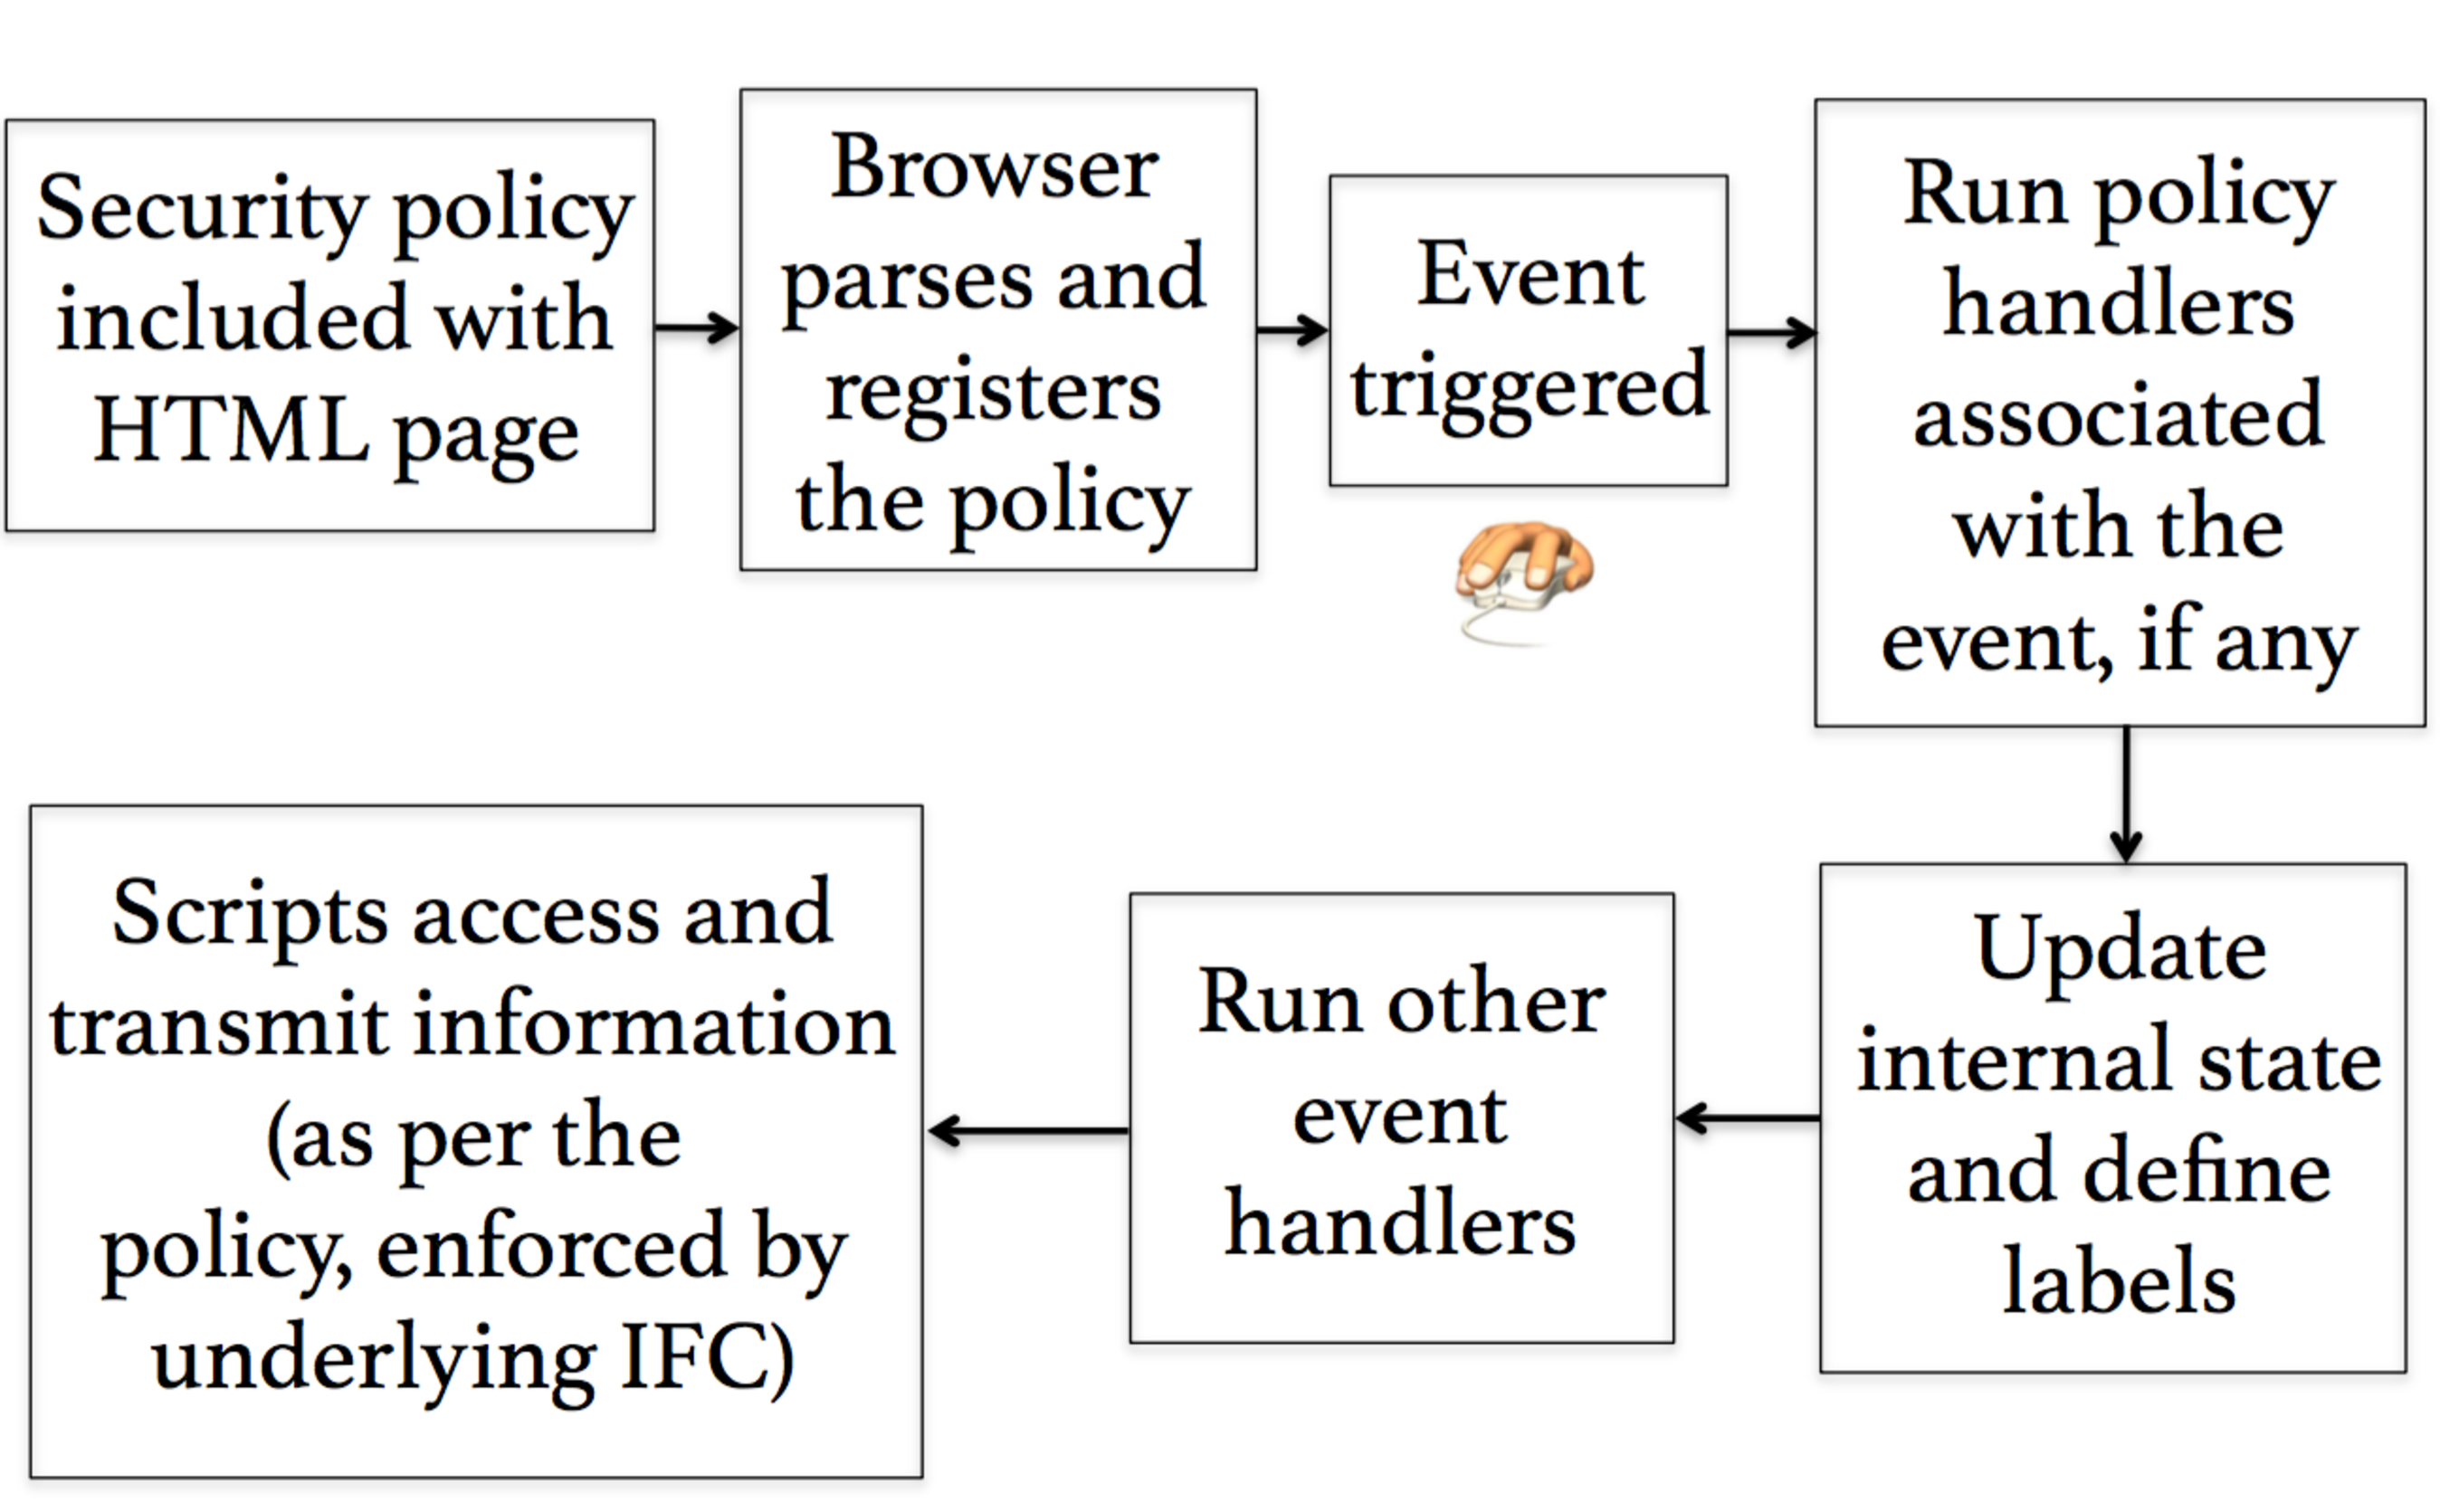
\includegraphics[width=8cm]{chapters/browser/webpol/Model.pdf} \caption{Workflow
  of the {\sys} policy model} \label{fig:model}
\end{figure}

Since different policy handlers can be associated with different
elements, Requirement~1 is satisfied.  Moreover, policy handlers are
ordinary JavaScript code, so they can also maintain local state in
private variables, thus satisfying Requirement~2. 

The workflow of policy interpretation in {\sys} is shown in
Figure~\ref{fig:model}. Briefly, the steps are:

\begin{enumerate}
\item The web page developer specifies the policy in the host HTML
  page in the form of special event handlers.
\item The browser parses the policy and registers its handlers (mostly
  like usual handlers, but with the two special privileges mentioned
  above).
\item When an event dispatches, listening policy handlers are
  executed first.
\item These policy handlers set labels on objects affected by the
  event, including the event object itself. They may also
  update any local state they maintain.
\item The remaining event handlers are dispatched as usual.
  The IFC enforcement in the browser enforces all labels that have
  been set by the policy handlers (during any prior event's dispatch),
  thus preventing any data leak in contravention of the labels.
\end{enumerate}

\subsection{Integration with the web browser}

{\sys} needs minor modifications to the browser to parse and interpret
policies and to expose additional JavaScript API functions to set
labels.

\medskip \noindent \textbf{HTML and event dispatch changes.}
{\sys} adds an HTML extension to differentiate policy code from other
JavaScript code. Concretely, the browser's parser is changed to
interpret any script file with the extension \texttt{.policy} included
directly in the host page as a policy. If such a \emph{policy script}
installs a handler, it is treated as a policy handler. Additionally, a
policy script can set labels on the page's global variables and DOM
elements (like password fields). If a script does this, it should be
included in the host page before third-party scripts that use those
variables. {\sys} also requires a small change to the browser's event
dispatch mechanism to execute policy handlers before other handlers.

\medskip \noindent \textbf{Label-setting APIs.}
{\sys} exposes two new JavaScript API functions to set labels. These
functions can be called only by the policy code in \texttt{.policy}
files and handlers installed by such files (the browser is modified to
enforce this).

The function \texttt{setLabel(label)} sets the label of the object on
which it is called to \texttt{label}. As explained
earlier, \texttt{label} can be \texttt{public}, a domain name,
or \texttt{local} (the default is \texttt{public}). Once an object's
label is set, it is enforced by the underlying IFC enforcement. The
special label \texttt{HOST} is a proxy for the domain of the host
page.

The function \texttt{setContext(label)} can be called only on an event
object. It restricts the \emph{visibility} of the event to
label \texttt{label} and higher. In simple terms, if \texttt{label} is
a domain, then only that domain can ever learn that this event
occurred, whereas if \texttt{label} is \texttt{local}, then no domain
can ever learn that this event occurred. Technically, this is
accomplished by setting the $\pc$ of the 
event handlers running during the dispatch to \texttt{label}, which
ensures that their side-effects (writes to DOM and network
communication) are labeled \texttt{label} or higher.

As opposed to \texttt{setLabel}, which makes individual data objects
(like password fields) private, \texttt{setContext} makes the
\emph{existence} of an event private. This is useful.
For instance, clicking on the ``politics'' section of a news feed
might indicate that the user is interested in politics, which may be
private information, so the page may want to hide even the existence
of click events from third-party scripts. (The distinction between the
privacy of event content and event occurrence has been previously
described by Rafnsson and Sabelfeld~\cite{Rafnsson-csf13}.)


\section{Expressiveness of {\sys}}
\label{sec:examples}

The expressiveness of {\sys} policies is illustrated through the
following examples.

\begin{lstlisting}[float, caption=Password strength checking script that leaks the password,label=egscript1,language=C]
var p = document.getElementById("pwd");
p.addEventListener("keypress", function (e){
  var score = checkPwdStrength(p.value);
  document.getElementById("pwdStrength").innerText = score; 
  new Image().src = "http://stealer.com/pwd.jsp?pwd="+p +score;
});
\end{lstlisting}

\subsection{Example 1: Password strength checker}  
Many websites deploy \emph{password strength checkers} on pages where
users set new passwords. A password strength checker is an event
handler from a third-party library that is triggered each time the
user enters a character in the new password field. The handler
provides visual feedback to the user about the strength of the
password entered so far. Strength checkers usually check the length of
the password and the diversity of characters used. Consequently, they
do not require any network communication. However, standard browser
policies cannot enforce this and the password strength checker can
easily leak the password if it wants to. Listing~\ref{egscript1} shows
such a ``leaky'' password checker. The checker installs a listener for 
keypresses in the password field (line 2). In response to every
keypress, the listener delivers its expected functionality by checking
the strength of the password and indicating this to the user (lines 3,
4), but then it leaks out the password to \texttt{stealer.com} by
requesting an image at a URL that includes the password (lines 5, 6). 

With {\sys}, the developer of the host web-page can prevent any
exfiltration of the password by including the policy script:

\medskip
\texttt{document.getElementById("pwd").setLabel("HOST");}

\medskip 
\noindent This policy sets the label of the password field to the
host's own domain using the function
\texttt{setLabel()}. Subsequently, the IFC enforcement restricts all
outgoing communication that depends on the password field to the host.

Conceptually, this example is simple because it does not really
leverage the fine-granularity of {\sys} policies and fine-grained
dynamic IFC. Here, the third-party script does not need any network
communication for its intended functionality and, hence, simpler
confinement mechanisms that prohibit a third-party script from
communicating with remote servers would also suffice. The next example 
is a scenario where the third-party script legitimately needs remote
communication, which leverages the fine-granularity of {\sys} policies
and fine-grained dynamic IFC.

\begin{lstlisting}[float, caption=Currency converter script that leaks a private amount,label=egcc,escapechar=\%]
function currencyConverter() {
	var toCur = document.getElementById("to").value;
	var xh = new XMLHttpRequest();
	xh.onreadystatechange = function() { %\label{startcallback}%
		if (xh.readyState == 4) { %\iffalse && xhttp.status == 200 \fi %
			currencyRate = eval(xhttp.responseText);%\label{startsend}%
			var aAmt = document.getElementById("amt").value;
			var convAmt = aAmt * currencyRate;
			document.getElementById("camt").innerHTML = convAmt;%\label{ressend}%
			xh.open("GET","http://currConv.com/amount.jsp?atc=" + aAmt);%\label{endsend}%
			xh.send(); }} %\label{endcallback}%
	xh.open("GET","http://currConv.com/conv.jsp?toCur=" + toCur, true);
	xh.send(); }
\end{lstlisting}


\subsection{Example 2: Currency conversion}
Consider a web-page from an e-commerce website which displays the cost
of an item that the user intends to buy. The amount is listed in the
site's native currency, say US dollars (USD), but for the user's
convenience, the site also allows the user to see the amount converted
to a currency of his/her choice. For this, the user selects a currency
from a drop-down list. A third-party JavaScript library reads both the
USD amount and the second currency, converts the amount to the second
currency and inserts it into the web-page, next to the USD amount.
%
The third-party script fetches the current conversion rate from its
back-end service at \texttt{currConv.com}. Consequently, it must send
the \emph{name} of the second currency to its back-end service, but
must not send the amount being converted (that is private
information). The web browser's same-origin policy has been relaxed
(using, say, CORS~\cite{cors}) to allow the script to talk to its
back-end service at \texttt{currConv.com}. The risk is that the script
can now exfiltrate the private amount. Listing~\ref{egcc} shows a
leaky script that does this. On line~\ref{endcallback}, the script
makes a request to its back-end service passing to it the two
currencies. The callback handler (lines
\ref{startcallback}--\ref{endcallback}) reads the amount from the page
element \texttt{amt}, converts it and inserts the result into the page
(lines \ref{startsend}--\ref{ressend}). Later, it leaks out the amount
to the back-end service on line~\ref{endsend}, in contravention of the
intended policy.

With {\sys}, this leak can be prevented with the following policy that
sets the label of the amount to the host only:

\medskip
\texttt{document.getElementById("amt").setLabel("HOST")}

\medskip
\noindent This policy will prevent exfiltration of the amount and will not
interfere with the requirement to exfiltrate the second
currency. Importantly, no modifications are required to a script that
does not try to leak data (e.g., the script obtained by dropping the
leaky line~\ref{endsend} of Listing~\ref{egcc}).

\begin{lstlisting}[float,caption=Policy that allows counting clicks but hides details of the clicks,label=eganal1]
var p = document.getElementbyId("sect_name");
p.addEventListener("click",function(event){
  event.setLabel("HOST"); });
\end{lstlisting}

\subsection{Example 3: Web analytics} 
To better understand how
users interact with their websites, web developers often include
third-party analytics scripts that track user clicks and keypresses to
generate useful artifacts like page heat-maps (which part of the page
did the user interact with most?). Although a web developer might be
interested in tracking only certain aspects of their users'
interaction, the inclusion of the third-party scripts comes with the
risk that the scripts will also record and exfiltrate other private
user behavior (possibly for monetizing it later). Using {\sys}, the
web developer can write precise policies on which user events an
analytics script can access and when. Several examples of this are
shown. 

\begin{lstlisting}[float, caption=Analytics script that counts clicks,label=egan]
clickCount = 0;
var p = document.getElementbyId("sect_name");  
p.addEventListener("click",function (e){ clickCount += 1; });
\end{lstlisting}

To allow a script to only count the number of occurrences of a class
of events (e.g., mouse clicks) on a section of the page, but to hide
the details of the individual events (e.g., the coordinates of every
individual click), the web developer can add a policy handler on the
top-most element of the section to set the label of the individual
event objects to \texttt{HOST}. This prevents the analytics script's
listening handler from examining the details of individual events, but
since the handler is still invoked at each event, it can count their
total number. Listings~\ref{eganal1} and~\ref{egan} show the policy
handler and the corresponding analytics script that counts clicks in a
page section named \texttt{sect\_name}.

\begin{lstlisting}[float,caption=Policy that only tracks whether a click
  happened or not,label=eganal2]
var alreadyClicked = false;
var p = document.getElementById("sect_name");
p.addEventListener("click",function (event){
  if (alreadyClicked = true) 
     event.setContext("HOST");
  else {
     alreadyClicked = true; 
     event.setLabel("HOST");
}});
\end{lstlisting}

Next, consider a restriction of this policy, which allows the
analytics script to learn only whether or not \emph{at least one}
click happened in the page section, completely hiding clicks beyond
the first. This policy can be represented in {\sys} using a local
state variable in the policy to track whether or not a click has
happened and the function \texttt{setContext()}. Listing~\ref{eganal2}
shows the policy. The policy uses a variable \texttt{alreadyClicked}
to track whether or not the user has clicked in the section. Upon the
user's first click, the policy handler sets the event's label to the
host's domain (line~8). This makes the event object private but allows
the analytics handler to trigger and record the occurrence of the
event. On every subsequent click, the policy handler sets the event's
\emph{context} to the host domain using \texttt{setContext()}
(line~5). This prevents the analytics script from exfiltrating any
information about the event, including the fact that it occurred.

Finally, note that a developer can subject different page sections to
different policies by attaching different policy handlers to them. The
most sensitive sections may have a policy that unconditionally sets
the event context to the host's, effectively hiding all user events in
those sections. Less sensitive sections may have policies like those
of Listings~\ref{eganal2} and~\ref{eganal1}. Non-sensitive sections
may have no policies at all, allowing analytics scripts to see all
events in them.

\begin{lstlisting}[float, caption=Example policy to prevent overlay-based
  stealing of keystrokes,label=overlay,language=C]
document.body.addEventListener("keypress", function (event){
    var o = window.getComputedStyle(event.target).getPropertyValue("opacity");
    if (o < 0.5) 
         event.setLabel("HOST");
});
\end{lstlisting}

\subsection{Example 4: Defending against overlay-based attacks}
To bypass {\sys} policies, an adversarial script may ``trick'' a user
using transparent overlays. For example, suppose a script wants to
exfiltrate the contents of a password field that is correctly
protected by a {\sys} policy. The script can create a transparent
overlay on top of the password field. Any password the user enters
will go into the overlay, which \emph{isn't} protected by any policy
and, hence, the script can leak the password.

Such attacks can be prevented easily in {\sys} using a \emph{single}
policy, attached to the top element of the page, that labels data
entered into all significantly transparent overlays as
\texttt{HOST}. Listing~\ref{overlay} shows such a policy. This
particular policy labels all keypress events on elements of opacity
below $0.5$ as \texttt{HOST}, thus preventing their exfiltration. The
threshold value $0.5$ can be changed, and the policy can be easily
extended to other user events like mouse clicks.

\subsection{Summary of {\sys} expressiveness} 
The security community has extensively studied several
aspects of policy labeling, colloquially called the \emph{dimensions
  of declassification} (see~\cite{dimDecl} for a survey). Broadly
speaking, {\sys} policies cover three of these dimensions---the
policies specify what data is declassified (dimension: what), to which
domains (dimension: to whom) and under what state (dimension:
when). ``What data is declassified'' is specified by selectively
attaching policies to elements of the page. ``Which domains get
access'' is determined directly by the labels that the policy
sets. Finally, labels generated by policy handlers can depend on
state, as illustrated in Listing~\ref{eganal2}.

There are two other common dimensions of labeling---who can label the
data (dimension: who) and where in the code can the labels change
(dimension: where). These dimensions are fixed in {\sys} due to the
specifics of the problem: All policies are specified by the host page
in statically defined policies.



\chapter{Policy Implementation and Evaluation in an IFC-enabled Browser}
\label{ch:eval}
\blfootnote{The content of this
  chapter is based partly on the work published as part of the paper,
  ``WebPol: Fine-grained Information Flow Policies for Web Browsers''~\cite{webpol}} 

This chapter describes the implementation of \sys~(Chapter~\ref{ch:webpol}) 
and the LIR policy (Chapter~\ref{ch:lir}) on top of
an existing IFC-instrumentation~\cite{just11PLASTIC,post14,csf15}. 
Their work instrumented WebKit, the browser engine used in Safari, for enforcing 
dynamic IFC in the three main components of the engine --- JavaScript 
bytecode interpreter, the document object model (DOM) engine, and the
event handling mechanism. 

Labels in their instrumentation are word size bit-sets (currently 64 
bits); each bit in the bit-set represents label from a distinct domain
(like google.com). Join on labels is simply bitwise or. Their
instrumentation adds labels to all data structures, including
registers, objects, object properties and scope chain pointers. They 
attach security labels to every node in the DOM graph and all its 
properties, including pointer to other nodes. 
They instrument the code to propagate explicit and implicit labels 
and implement the permissive-upgrade check. 

They instrument WebKit’s JavaScript bytecode interpreter (JavaScriptCore) 
for enforcing dynamic IFC for JavaScript~\cite{just11PLASTIC,post14}. 
In WebKit, bytecode is generated
by a source-code compiler and organized into code blocks. Each code
block is a sequence of bytecodes with line numbers and corresponds to
the instructions for a function or an \texttt{eval} statement. A code
block is generated when a function is created or an \texttt{eval} is
executed. Their instrumentation performs control flow analysis on a
code block when it is created and generates a CFG for it before it
starts executing. The IPDs of its nodes are calculated by static
analysis of its bytecode; they are computed using an algorithm by
Lengauer and Tarjan with CFG as an input to the
algorithm~\cite{Lengauer}. The formalization of the bytecodes, the
semantics of its bytecode interpreter with the instrumentation of
dynamic IFC, and the proof of correctness of instrumentation of the
bytecodes with the IFC semantics is shown in~\cite{post14Extended}.
Additionally, all native JavaScript methods in the Array, RegExp, 
and String objects are instrumented and appropriate  
IFC checks in the native C code implementing all DOM APIs up
to Level 3 are added~\cite{csf15}. 
They also modify the event handling loop, labeling every event and
event handler based on their formalization of the event handling loop
with the IFC checks~\cite{csf15}.  

Their work enforces IFC soundly in all the major components of 
a web browser while tracking labels at a fine-granularity. This thesis 
builds on top of their instrumentation for enforcing the ideas presented 
earlier. For exceptions, a synthetic exit node is added to the CFG
along with the edges as described earlier in
Section~\ref{sec:excsen}. Additional changes are required to the
compiler to make it compliant with the instrumentation. The
modification is to emit a slightly different, but functionally
equivalent bytecode sequence for \texttt{finally} blocks; 
this is needed for accurate computation of IPDs. 


\section{Implementation and Evaluation of \sys}
\label{sec:implpol}
\subsection{Implementation of \sys}
{\sys} is prototyped in WebKit on top of the prior IFC enforcement in
WebKit described above~\cite{just11PLASTIC,post14,csf15}. To implement
{\sys}, the HTML parser was modified to distinguish policy files
(extension \texttt{.policy}) from other JavaScript files and to give
policy code extra privileges. Two new JavaScript API functions ---
\texttt{setLabel()} and \texttt{setContext()} --- were added. Finally,
the event dispatch logic was modified to trigger policy handlers
before other handlers. In all, 25 lines in the code of the parser were
modified, 60 lines for the two new API functions were added and 110
lines in the event dispatch logic were modified. Thus, implementing
{\sys} has low overhead, and can be ported to other browsers easily.

\subsection{Evaluation of \sys}
\label{sec:eval-webpol}
The goal of the evaluation is two-fold. The first goal is to measure
the overhead of the system with IFC enforcement and {\sys}, both in
parsing and installing policies during page load and for executing
policy handlers later. This is done by running a few benchmarks, by measuring the
overhead for the examples presented in Chapter~\ref{sec:examples}, and
for two real-world websites. Second, to 
understand whether {\sys} can be used easily, {\sys} policies are
applied to two real-world websites. All the experiments were
performed on a 3.2GHz Quad-core Intel Xeon processor with 8GB RAM,
running Mac OS X version 10.7.4 using Safari 6.0. The implementation
and evaluation is done on WebKit nightly build $\#r122160$. As the
existing IFC instrumentation does not handle JIT, JIT support was
disabled in all the experiments. 

\subsubsection{Performance Overheads on Synthetic Examples}
To measure the instrumentation's runtime overhead, four examples from 
Chapter~\ref{sec:examples} (Examples~1,~2 and the two sub-examples of
Example~3) were tested in three different configurations:
\textbf{Base}---uninst\-ru\-mented browser, no enforcement;
\textbf{IFC}---existing instrumented browser with IFC checks, but no
policy handlers (everything is labeled public);
\textbf{{\sys}}---instrumented browser running policy handlers.

\newcolumntype{C}[1]{>{\centering\let\newline\\\arraybackslash\hspace{0pt}}m{#1}}

\begin{table}[tbp]
\centering
\begin{tabular}{ | C{2cm} || C{1.5cm} | C{1.5cm} | C{1.5cm} || C{1.5cm} | C{1.5cm} | C{1.5cm} |}
\hline
\multicolumn{1}{|c||}{ } &
\multicolumn{3}{ c ||}{JavaScript Execution Time} &
\multicolumn{3}{ c |}{Page Load Time} \\
\hline
 Example \# & \textbf{Base} & \textbf{IFC} & \textbf{\sys} & \textbf{Base} & \textbf{IFC} & \textbf{\sys} \\
  \hhline{|=#=|=|=#=|=|=|} 
  Example~1 & 2430 & 2918 (+20.1\%) & 2989 (+1.9\%) & 16 & 17 (+6.3\%) & 19 (+12.5\%) \\  
\hline
  Example~2 & 3443 & 4361 (+26.7\%) & 5368 (+29.2\%) & 41 & 43 (+4.9\%) & 46 (+7.2\%)\\ 
\hline
  Example~3 (count) & 1504 & 1737 (+15.5\%) & 1911 (+11.6\%) & 24 & 25 (+4.2\%) & 31 (+25.0\%) \\
\hline
  Example~3 (presence) & 1780 & 2095 (+17.7\%) & 2414 (+18.9\%) & 26 & 28 (+7.7\%) & 30 (+7.7\%)\\
\hline
\end{tabular}
\caption{Performance of examples from Section~\ref{sec:examples}. All
  time in ms. The numbers in parenthesis are additional overheads
  relative to \textbf{Base}.}
\label{table:eap}
\end{table}

\noindent
\textbf{JavaScript execution time:} The overheads of executing policy
handler code were measured by interacting with all four programs
manually by entering relevant data and performing clicks a fixed
number of times. For each of these configurations, the total time
spent \emph{only in executing JavaScript} was measured, including 
scripts and policies loaded initially with the page and the scripts
and policies executed in response to events. The difference between
\textbf{IFC} and \textbf{Base} run times is the overhead of dynamic
IFC, while the difference between the \textbf{\sys} and
\textbf{IFC} run times is the overhead of evaluating policy
handlers. Since only JavaScript execution time is measured and
there are no time-triggered handlers in these examples, variability in
the inter-event gap introduced by the human actor does not affect the
measurements.

The left half of Table~\ref{table:eap} shows these observations.
%
All numbers are averages of 5 runs and the standard deviations are
all below 7\%. %\TODO{Fill these numbers}
%
Taint-tracking (\textbf{IFC}) adds overheads ranging from 15.5\% to
26.7\% over \textbf{Base}. To this, policy handlers (\textbf{\sys})
adds overheads ranging from 1.9\% to 29.2\%. The \textbf{\sys}
overheads are already modest, but this is also a very challenging
(conservative) experiment for {\sys}. The scripts in 
both sub-examples of Example~3 do almost nothing. The scripts in
Examples~1 and Example~2 are slightly longer, but are still much
simpler than real scripts. On real and longer scripts, the relative
overheads of evaluating the policy handlers is significantly lower as
shown later. Moreover, the baseline in this experiment does not
include other browser costs, such as the cost of page parsing and
rendering, and network delays. Compared to those, both \textbf{IFC}
and \textbf{\sys} overheads are negligible.

\noindent
\textbf{Page load time:} The time taken for loading the initial page
(up to the DOMContentLoaded event) was measured separately. The
difference between \textbf{sys} and \textbf{IFC} is the overhead for
parsing and loading policies. The right half of Table~\ref{table:eap}
shows these observations. All numbers are the average of 20 runs and
standard deviations were below 8\%.
{\sys} overheads due to policy parsing and loading range from 7.2\% to
25\% (last column). When the overheads due to taint tracking
(column \textbf{IFC}) are added, the numbers increase to 12.1\% to
29.2\%. Note that page-load overheads are incurred only once on every
page (re-)load. 

\subsubsection{Policies on Real-world Websites.}
\label{sec:realpolicies}

Further, {\sys} was evaluated by writing policies for two real-world
applications---a website that deploys a password-strength checker
(similar to Example~1) and a bank login page that includes third-party
analytics scripts (similar to Example~3).
The {\sys} policies specified for the password strength checking
website and the bank website with an analytics script are shown in
Listings~\ref{realpolicy1} and~\ref{realpolicy2}, respectively. The
code on lines~\ref{ex:start}--\ref{ex:end} of
Listing~\ref{realpolicy1} allows the strength-checking script to write
back the visual indicator of password strength to the host page's DOM.

\begin{lstlisting}[float, caption=Policy code for password strength
  checking website,label=realpolicy1,language=C,escapechar=\%]
document.getElementById("passwordPwd").setLabel("secret");
document.getElementById("passwordTxt").setLabel("secret");
var x = document.getElementsByTagName("div"); %\label{ex:start}%
var i = 0;
for (i = 0; i < x.length; i++) 
    x[i].setLabel("secret"); %\label{ex:end}%
\end{lstlisting}

\begin{lstlisting}[float, caption=Policy code for bank login
  website with an analytics script,label=realpolicy2,language=C] 
var x = document.getElementsByClassName("user"); // username
var y = document.getElementsByClassName("pwd"); // password
for (i = 0; i < x.length; i++) {
    x[i].addEventListener("keypress", function(event){
    event.setLabel("HOST");
    });}
for (i = 0; i < y.length; i++) {
    y[i].addEventListener("keypress", function(event){
    event.setLabel("HOST");
    });}
\end{lstlisting}

\noindent
\textbf{Experience writing policies:} In both cases, meaningful
policies could be specified easily after understanding the code,
suggesting that {\sys} policies can be (and should be) written by
website developers. The policy for the password-strength
checker is similar to Listing~\ref{egscript1} and prevents the
password from being leaked to third-parties. Additional policy code of
4 lines was needed to allow the script to write the results of
the password strength check (which depends on the password) into the
host page.
%
The analytics script on the bank website communicates all
user-behavior to its server.  The policy specified disallows
exfiltration of keypresses on the username and the password text-boxes 
to third-parties.

%% The policy, however, allows the script to exfiltrate mouse-clicks
%% on the text-boxes by default.

%% We evaluate {\sys} by running a couple of real-world applications -- a
%% password strength checker website, and a bank login web page including
%% third-party analytics, and the four programs shown in
%% Section~\ref{sec:examples} (Examples 1, 2 and the two sub-examples of
%% Example~3). 
%% For the password strength checking website, we added a policy
%% (Example~\ref{realpolicy1}) to protect the 
%% password from being leaked over the network (similar to the example in
%% Example~\ref{egscript1}). We were able to verify that the website
%% indeed did not send the password on the network.

%% The additional policy
%% code (lines~\ref{ex:start}--\ref{ex:end}) is required to allow the
%% script to write to the HTML document the score and other computed
%% information, which is dependent on the value of password. The bank
%% login website included a user-behavior tracking analytics 
%% script.


% \medskip\noindent\textbf{Real-world Applications.} We also compare the 
% performance of \textbf{\sys} on top of the taint tracking mechanism
% against an IFC-instrumented browser without policy handlers
% (\textbf{IFC})  and the uninstrumented browser (\textbf{Base}). We
% measure the average time taken to load the DOM 
% content (measured by the DOMContentLoaded event) for two real-world
% applications. In the case of \textbf{\sys}, the measure includes the time taken to parse, and load
% the policies along with the web page.  
% The length of the policy code in the
% two cases was 6 lines and 10 lines, respectively. The policy codes and
% their descriptions are listed in the Appendix. 

\begin{table}[tbp]
\centering
\begin{tabular}{ | C{2cm} || C{1.5cm} | C{1.5cm} | C{1.5cm} || C{1.5cm} | C{1.5cm} | C{1.5cm} |}
\hline
\multicolumn{1}{|c||}{ } &
\multicolumn{3}{ c ||}{JavaScript Execution Time} &
                                                       \multicolumn{3}{
                                                         c |}{Page Load Time} \\
\hline
 \multicolumn{1}{|c||}{Website} & \textbf{Base} & \textbf{IFC} & \textbf{\sys} & \textbf{Base} & \textbf{IFC} & \textbf{\sys} \\
\hhline{|=#=|=|=#=|=|=|} 
 \multicolumn{1}{|c||}{Password} & 79.5 & 115.5 (+45.3\%) & 126 (+13.2\%) & 303 & 429 (+41.6\%) & 441 (+4.0\%)\\  
\hline
 \multicolumn{1}{|c||}{Analytics} & 273.4 & 375.1 (+37.2\%) & 386.1 (+4.0\%) & 2151 & 2422 (+12.6\%) & 2499 (+3.6\%) \\ 
\hline
\end{tabular}
\caption{Performance on two real-world websites. All time in ms. The
  numbers in parenthesis are additional overheads relative to
  \textbf{Base}.}
\label{table:rap}
\end{table}

\noindent
\textbf{Performance overheads:} The performance overheads 
on the two websites were also measured, in the same configurations as
for the synthetic examples. Table~\ref{table:rap} shows the
results. On real-world websites, where actual computation is long, the
overheads of {\sys} are rather small. The overheads of executing
policy handlers, even relative only to \textbf{Base}'s JavaScript
execution time, are 4.0\% and 13.2\%, while the overheads of parsing
and loading policies are no more than 4.0\%. Even the total overhead
of \textbf{IFC} and \textbf{\sys} does not adversely affect the user
experience in any significant way.

% \subsection{User-study for {\sys}}

% To understand how easily programmers can use {\sys}, a small study
% with six students from the university was conducted, recruited through
% an open call.  All participants knew how to program as this skill was
% specifically asked for this in the call, but only four knew JavaScript well
% and of those four, two had studied information flow control
% previously. Each participant's goal was to write policies for four
% scenarios very similar to Examples~1,~2 and the two sub-examples of
% Example~3. The participants were given a document of approximately
% 2,000 words that explained {\sys} and its API, and provided an
% illustrative example. The participants were allowed to ask questions
% about the documentation. Then, the participants were given the code of
% the host pages and included third-party scripts for the four scenarios
% and were asked to implement policies. They did this on the running
% prototype and could see the consequences of their mistakes in
% real-time and could debug their policies. The participants had up to
% one hour to study the documentation and implement the policies.

% Although the study size is quite small to state results with statistical
% confidence, the observations tend to indicate that {\sys} can be used
% by JavaScript programmers with a bit of training. All participants
% were able to complete three of the four exercises. The two
% participants who knew about information flow control were able to
% complete all four exercises. The exercise that the remaining four
% participants could not complete involved context labels and
% \texttt{setContext()}. This is unsurprising, since context labels are
% a difficult concept, although they are not needed very often. The two
% participants who did not know JavaScript well encountered another
% policy independent hurdle: They did not know the syntax for writing
% JavaScript handlers. Once they were explained this syntax, they were
% able to write all policies except the one involving
% \texttt{setContext()}.

% Overall, this \emph{suggests} that JavaScript programmers should be
% able to use {\sys} with little training, except the context
% labels. With an understanding of how information flow tracking works,
% they should be able to use context labels as well.

\section{Implementation and Evaluation of LIR}
\label{sec:impllir}

To implement the LIR semantics described in Chapter~\ref{ch:lir}, the
security label attached to the JavaScript objects and the DOM nodes
was modified to carry a provenance label, representing the dependency
set. The provenance label is basically a bitvector where each bit
represents a distinct JavaScript object or DOM node. Each bit in the
provenance label is mapped to a budget, a budget label and an actual
label of the object. The \texttt{setLabel()} API is extended to
include the budget, and the budget label for a JavaScript object or a
DOM node. If the budget is not specified, it is assumed to be
$0$. Similarly, if a budget label is not specified, it is assumed to
be $\bot$. The checks are performed as per the semantics at every
comparison operation assuming an implicit declassification at 
each comparison operation.

The performance overhead added as part of the LIR instrumentation in
the IFC-enabled browser is evaluated and compared against the
uninstrumented browser and {\sys} without the LIR enforcement. 
The performance evaluation was done for the standard
SunSpider 1.0.2 JavaScript benchmark suite on the uninstrumented
browser, on the IFC-instrumented browser and on the LIR instrumented
browser. The average overhead for LIR instrumentation over the
original uninstrumented browser is 170\% and adds only 17\% to the
overhead of \sys.

% \subsection{Performance Overhead on Different Benchmarks}
% \begin{figure}
%   \centering
%     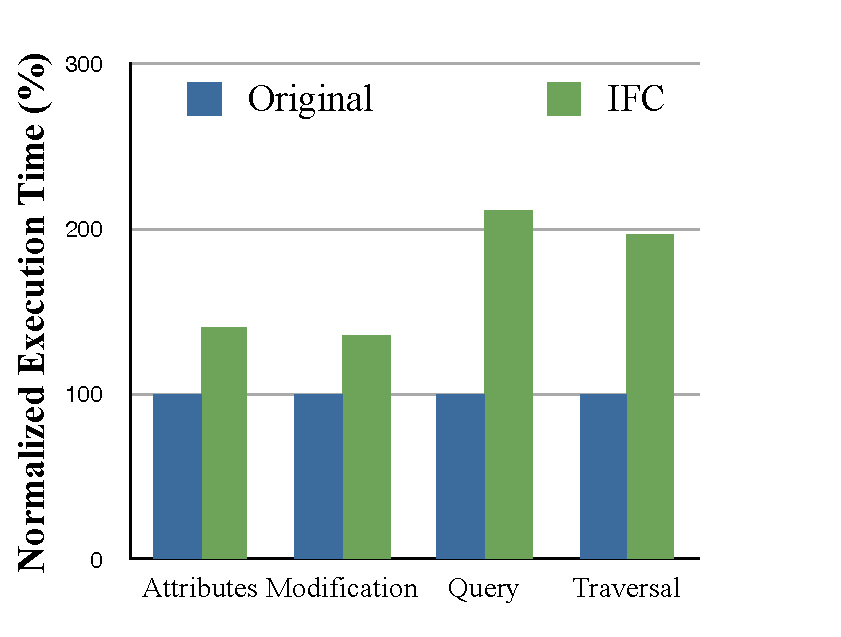
\includegraphics[width=0.8\linewidth]{chapters/browser/DOMCore.pdf}
%   \caption{Overheads of IFC on Dromaeo DOM Core Benchmark Tests}
%   \label{fig:dom}
% \end{figure}

% \begin{figure}
%   \centering
%     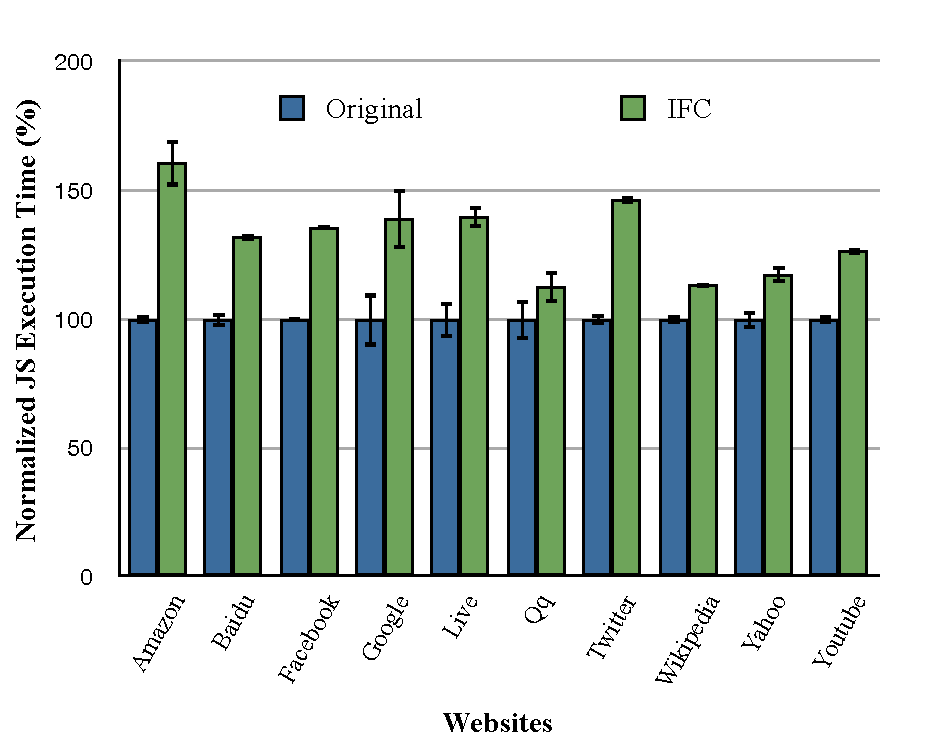
\includegraphics[width=\linewidth]{chapters/browser/Macro.pdf}
%   \caption{Overheads of IFC on Alexa Top 10 Websites}
%   \label{fig:macro}
% \end{figure}


% \begin{figure}
%   \centering
%     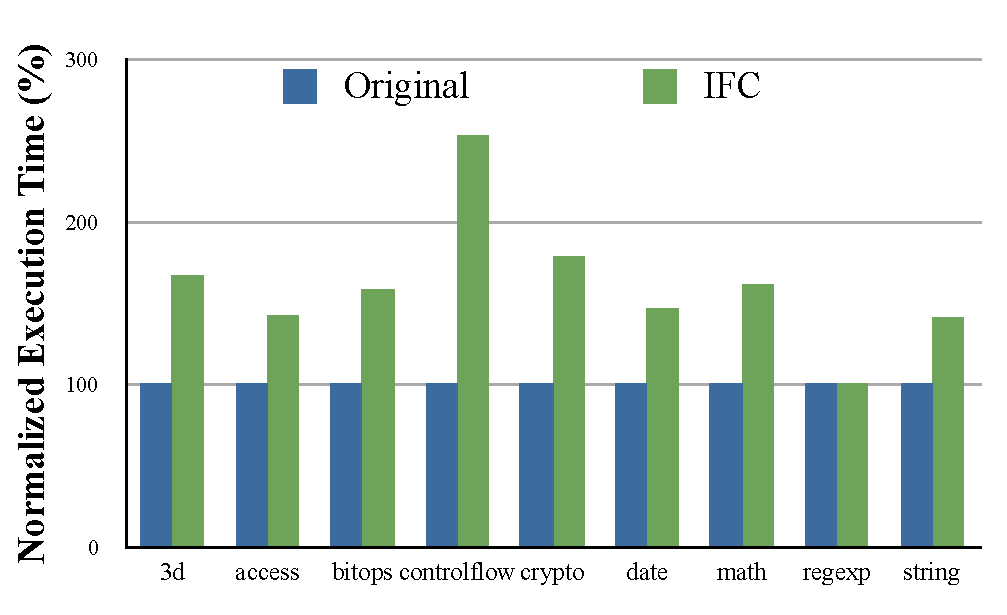
\includegraphics[width=\linewidth]{chapters/browser/SunSpider.pdf}
%   \caption{Overheads of IFC on SunSpider JavaScript Benchmark Tests}
%   \label{fig:js}
% \end{figure}

% The instrumentation is evaluated on the Dromaeo DOM Core
% benchmark~\cite{dromaeo}, which measures the performance of various
% operations on the DOM. The average overhead is approximately 71\% over
% the uninstrumented browser. Normalized overheads on different kinds of
% tests are shown in Figure~\ref{fig:dom} (standard deviations on
% individual tests were small, ranging from 0.17\% to 8.45\%). To get a
% more realistic evaluation, the instrumentation was also tested on the
% Alexa Top 10 websites~\cite{alexa}. The execution time of JavaScript
% was measured that loads initially on each website’s front page,
% without any user interaction. The graph in Figure~\ref{fig:macro}
% shows normalized execution time. Error bars are standard
% deviations. The average overhead is approximately 32\% and the worst 
% overhead is around 60\%. Note that both the Dromaeo and Alexa tests
% are very performance-intensive and do not count common browser delays
% like network communication and page rendering in the
% baseline. Compared to a baseline that includes these delays, our
% overheads are negligible. Finally, the very popular SunSpider
% benchmark~\cite{sunspider} was also run. SunSpider is a pure JS
% benchmark that does not cover events or the DOM. Results are shown in
% Figure~\ref{fig:js}. Although the overheads of IFC vary from test to
% test, the average overheads over the baseline uninstrumented
% interpreter is about 45\%. 

%% Tables~\ref{table:rap} and~\ref{table:eap} records the evaluation
%% results for the different applications in the three configurations. In 
%% general, the average overhead for page-load varies from 4.16\% to 40\% 
%% for \textbf{IFC}. \textbf{\sys} adds an overhead of about 2.79\% to
%% 29.16\% on top of it. The average overhead for JavaScript execution 
%% varies from 16\% to 83\% for \textbf{IFC} on top of
%% \textbf{Base}. To this overhead, the execution of
%% policy handlers (\textbf{{\sys}}) adds another 4\% to 29\%, relative
%% to \textbf{Base}. (See Appendix for a detailed analysis of the evaluation.)

% Table~\ref{table:rap} records the evaluation results for the
% real-world applications in the three configurations. In 
% general, the average overhead for page-load varies from 13\% to 40\%
% for \textbf{IFC}. \textbf{\sys} adds a small overhead of about 2.79\% to
% 3.18\% on top of it. 

% Table~\ref{table:eapl} shows the results for the four example programs.
% The overhead of the page load time of \textbf{IFC} with respect to
% \textbf{Base} varies from 4.16\% to 7.69\%. The overhead added
% by \sys with respect to \textbf{Base} varies from 12.19\% to
% 29.16\%. The average overhead for JavaScript execution 
% varies from 16\% to 83\% for \textbf{IFC} on top of
% \textbf{Base}. To this overhead, the execution of
% policy handlers (\textbf{{\sys}}) adds another 13\% to 29\%, relative
% to \textbf{Base}. 

% The average time for loading the website (over 20 runs) on
% \textbf{Base} was 303 ms with a standard deviation of about 3.58\%. For
% \textbf{IFC}, the average time was 429 ms with a standard deviation of
% about 2.3\% adding an overhead of about 41.5\% over
% \textbf{Base}. The average time for loading the website including the
% policy (\textbf{\sys}), was 441 ms with a standard deviation of about
% 3.82\%. The ovehead of \textbf{\sys} over \textbf{Base} is 45.5\%
% and over \textbf{IFC} is just 2.79\%.

% The average time for loading the website (over 20 runs) on
% \textbf{Base} was 2151 ms with a standard deviation of about 2.59\%. For
% \textbf{IFC}, the average time was 2422 ms with a standard deviation of
% about 1.08\% adding an overhead of about 12.59\% over
% \textbf{Base}. The average time for loading the website including the
% policy (\textbf{\sys}), was 2499 ms with a standard deviation of about
% 3.02\%. The ovehead of \textbf{\sys} over \textbf{Base} is 16.17\%
% and over \textbf{IFC} is 3.18\%.

% \TODO{Figure in appendix now}

%% \begin{table}[tbp]
%% \centering
%% \begin{tabular}{ | C{2cm} || C{1.5cm} | C{1.5cm} | C{1.5cm} || C{1.5cm} | C{1.5cm} | C{1.5cm} |}
%% \hline
%% \multicolumn{1}{|c||}{ } &
%% \multicolumn{3}{ c ||}{JavaScript Execution Time} &
%%                                                        \multicolumn{3}{
%%                                                          c |}{Page Load Time} \\
%% \hline
%%  \multicolumn{1}{|c||}{Applications} & Base & IFC & \sys & Base & IFC & \sys \\
%% \hhline{|=#=|=|=#=|=|=|} 
%%  \multicolumn{1}{|c||}{Password} & 79.5 & 115.5 & 126 & 303 & 429 & 441 \\  
%% \hline
%%  \multicolumn{1}{|c||}{Analytics} & 273.4 & 375.1 & 386.1 & 2151 & 2422 & 2499 \\ 
%% \hline
%% \end{tabular}
%% \caption{Real Applications Performance (time in ms)}
%% \label{table:rap}
%% \end{table}

% \begin{table}
% \centering
% \begin{tabular}{ | c | c | c | c |}
% \hline
%  Applications & Base & IFC & \sys \\
% \hline
% \hline
%   Analytics & 2151 & 2422 & 2499 \\ 
% \hline
%   Password & 303 & 429 & 441 \\  
% \hline
% \end{tabular}
% \caption{Real applications - Page Load Time (in ms)}
% \label{table:rapl}
% \end{table}

%% \begin{table}[tbp]
%% \centering
%% \begin{tabular}{ | C{2cm} || C{1.5cm} | C{1.5cm} | C{1.5cm} || C{1.5cm} | C{1.5cm} | C{1.5cm} |}
%% \hline
%% \multicolumn{1}{|c||}{ } &
%% \multicolumn{3}{ c ||}{JavaScript Execution Time} &
%% \multicolumn{3}{ c |}{Page Load Time} \\
%% \hline
%%  Example Applications & Base & IFC & \sys & Base & IFC & \sys \\
%%   \hhline{|=#=|=|=#=|=|=|} 
%%   PSC & 2430 & 2918 & 2989 & 16 & 17 & 19 \\  
%% \hline
%%   Converter & 3443 & 4361 & 5368 & 41 & 43 & 46 \\ 
%% \hline
%%   Presence & 1504 & 1737 & 1911 & 24 & 25 & 31 \\
%% \hline
%%   Coordinate & 1780 & 2095 & 2414 & 26 & 28 & 30 \\
%% \hline
%% \end{tabular}
%% \caption{Example Applications Performance (time in ms)}
%% \label{table:eap}
%% \end{table}

% \begin{table}
% \centering
% \begin{tabular}{ | c | c | c | c |}
% \hline
%  Example Applications & Base & IFC & \sys \\
% \hline
% \hline
%   Currency Converter & 3443 & 4361 & 5368 \\ 
% \hline
%   Password Strength Checker & 2430 & 2918 & 2989 \\  
% \hline
%   Presence & 1504 & 1737 & 1911 \\
% \hline
%   Coordinate & 1780 & 2095 & 2414 \\
% \hline
% \end{tabular}
% \caption{Example applications - JavaScript Execution Time (in ms)}
% \label{table:eapl}
% \end{table}

% Figure~\ref{fig:perf} shows the JavaScript execution times averaged
% over five runs for each program in each configuration. Standard
% deviations were small, no more than 3\%, except in the currency
% converter {\textbf{\sys}} line (7\%). 
% The overhead of taint tracking
% (\textbf{IFC}) over the baseline (\textbf{Base}) varies from 16\% in
% analytics presence to 83\% in password strength. This overhead is
% higher for scripts that perform more arithmetic and logical operations
% and our measurements are consistent with those from our prior work,
% which measured the same overhead on standard benchmarks~\cite{post14,csf15}. 
% To this overhead, the execution of
% policy handlers (\textbf{{\sys}}) adds another 13\% to 29\%, relative
% to \textbf{Base}. This policy overhead is proportional to the ratio of
% the work done in the policy code to other JavaScript. Most of the cost
% in policy code comes from executing native functions like
% \texttt{getElementbyId()}, which is used to find the DOM element whose
% label must be set or to which a policy handler must be attached. The
% figure plotting the JavaScript execution times for each of the examples
% is included in the Appendix.

% We note that this is a very challenging baseline for {\sys} and the
% experiment measures overheads very conservatively. The scripts in both
% sub-examples of Example~3 do almost nothing. The scripts in Examples~1
% and Example~2 are slightly longer, but are still much simpler than
% real scripts. On real, and longer scripts, the relative overheads of
% evaluating the policy handlers will be significantly lower. Moreover,
% our baseline does not include other browser costs, such as the cost of
% parsing, page loading and rendering, and network delays. In fact, the
% overheads induced by both taint tracking and policy handlers are too
% small to be perceived by the browser's user. They do not exceed 2.56ms
% across all interactions in any of the four experiments.

% The overhead of the page load time of \textbf{IFC} with respect to
% \textbf{Base} is 4.8\%, 6.25\%, 4.16\%, and 7.69\%. The overhead added
% by \sys with respect to \textbf{Base} is 12.19\%, 18.75\%, 29.16\%,
% and 15.38 \%. 

% The standard deviation varies from 2.3 \% to 4.3 \% for
% \textbf{Base}, 2.85\% to 4.17\% for \textbf{IFC} and 3.6\% to 7.4\%
% for \sys.

%% The performance measure are performed on
%% on a 3.2GHz Quad-core Intel Xeon processor with 8GB RAM, running Mac OS X
%% version 10.7.4. We extend our previous instrumentation of taint tracking
%% from~\cite{csf15} which is based on WebKit build \#r122160 and works with the
%% Safari web browser, version 6.0. As the major changes to the browser were
%% confined to the event handling mechanism of the browser, running the JavaScript
%% benchmarks produced a similar moderate performance overhead as shown in our
%% earlier work. The additional overhead of executing the policy code is dependent
%% on the size of the policy code. We perform two kinds of performance experiments.

%% First, we measure the overhead of taint tracking by running our examples (not
%% containing policy) on the instrumented browser against the same examples (not
%% containing policy) on the unmodified browser. As can be seen in
%% Figure~\ref{fig:taintOverhead} the average percentage overhead of taint tracking
%% is around ...

%% Second, we measure the overhead due to the changes introduced by the inlcusion
%% of the policy. The average percentage overhead per example is shown in
%% Figure~\ref{fig:policyOverhead}.

% The average time for
% loading the two websites on \textbf{Base} was 356.2 ms and 2196.4 ms, 
% respectively, and with \textbf{\sys}, the average time for loading the
% two websites along with the policies was 415 ms and 2477 ms,
% respectively.  


%% To evaluate the practicality and usability of the model, we conducted
%% an anecdotal study with a few students from the university. The
%% students were given a set of four exercises (based on the examples
%% presented before) to write security policies for and the documentation
%% related to the additional set of APIs that they could use for specifying these
%% policies. They also had access to a running prototype of our
%% implementation where they could check the policies specified by them
%% against the requirement. To summarise the results: we found that the
%% students who were knowledgable with JavaScript and HTML programming
%% and did not have any prior knowledge of information flow control
%% were able to specify correct policies for almost all exercises with
%% the exception of those that required the execution context to be
%% set. The students who had knowledge of both information flow
%% control and JavaScript and HTML programming were able to specify
%% correct policies for all the exercises. The students who had basic
%% knowledge of programming with JavaScript and HTML but had knowledge of
%% IFC weren't able to specify the correct policy in one out of the four
%% cases that required a non-trivial JavaScript specification. The other
%% major problem which the students had was that the documentation was
%% not extensive enough but with some discussion they were able to
%% understand the functionality of the model better. Overall, we found
%% that the specification of policies would in general require a good
%% knowledge of JavaScript and HTML programming but very basic knowledge
%% of IFC, which evaluates the usability of our model positively
%% considering the fact that web developers only need to have some basic
%% training of IFC to be able to specify the required security policies.

\chapter{Related Work}
\label{ch:related}

Browser security is a very widely-studied topic. Here, only closely
related work on information flow control for browsers, browser
security policies and policy enforcement techniques is described. 

\medskip\noindent\textbf{Information flow control and script
  isolation.} With the widespread use of JavaScript,
research in dynamic techniques for IFC has regained momentum.
Nonetheless, static analyses are not completely futile. Guarn\-ieri
\emph{et al.}~\cite{guarnieri11ISSTA} present a static abstract
interpretation for tracking taints in JavaScript. However, the
omnipresent \texttt{eval} construct is not supported and this approach
does not take implicit flows into account.  Chugh \emph{et al.}
propose a staged information flow approach for 
JavaScript~\cite{stagedIFC}. They perform static server-side policy
checks on statically available code and generate residual
policy-checks that are applied to dynamically loaded code.  This
approach is limited to certain JavaScript constructs excluding dynamic 
features like dynamic field access or the \texttt{with} construct.

Austin and Flanagan~\cite{plas09} propose purely dynamic IFC for
dynamically-typed languages like JavaScript. They use the
no-sensitive-upgrade (NSU) check~\cite{zdancewic02PhD} to handle
implicit flows. Their per\-mis\-sive-upgrade strategy~\cite{plas10} is
more permissive than NSU but retains ter\-mi\-na\-tion-insensitive
non-interference. This work builds on the permissive-upgrade
strategy. They also present faceted evaluation~\cite{austin12POPL},
which is the most permissive technique of the three. However, given
the performance considerations, the technique is not suitable for
enforcing information flow control in browsers.  Just
et al.~\cite{just11PLASTIC} present dynamic IFC for JavaScript
bytecode with static analysis to determine implicit flows precisely
even in the presence of semi-unstructured control flow like
\texttt{break} and \texttt{continue}. Again, NSU is leveraged to
prevent implicit flows. This thesis builds on top of their work to
enforce information flow control in browsers.

JSFlow~\cite{csf12,jsflow} is a stand-alone implementation of
a JavaScript interpreter with fine-grained taint tracking. Many
seminal ideas for labeling and tracking flows in JavaScript owe their
lineage to JSFlow, but since JSFlow is written from scratch it has
very high overheads and  introduces annotations to deal with
semi-structured control flow. It detects
security violations due to branches that have not been executed and
injects annotations to prevent these in subsequent runs. The approach
presented in this thesis relies on analyzing CFGs and does not require
annotations. To improve permissiveness,
their subsequent work~\cite{esorics12} uses testing. 

Kerschbaumer et al.~\cite{crowdflow} build an implementation of an
information flow monitor for WebKit but do not handle all implicit
flows.  A black-box approach to enforcing non-interference is based on
secure multi-execution (SME)~\cite{SME}. Bielova \emph{et
  al.}~\cite{rnib} and De Groef \emph{et al.}~\cite{flowfox} implement
SME for web browsers. These systems do not attach labels to specific
fields in the DOM. Instead, labels are attached to individual DOM
APIs.

Chudnov and Naumann~\cite{chudnov-ccs} present another approach to
fine-grained IFC for JavaScript. They rewrite source programs to add
shadow variables that hold labels and additional code that tracks
taints. This approach is inherently more portable than that of JSFlow
or the work presented in this thesis, both of which are tied to
specific, instrumented browsers. However, it is unclear how this
approach could be extended with a policy framework like {\sys} that
assigns state-dependent labels at runtime.

The work most closely related to $\sys$ is that of
Vanhoef \emph{et al.}~\cite{csf14} on stateful declassification
policies in reactive systems, including web browsers. Their policies
are similar to the ones presented here, but there are significant
differences. First, 
their policies are attached to the browser and they are managed by the
browser user rather than website developers. Second, the policies have 
coarse-granularity: They apply uniformly to all events of a certain
type. Hence, it is impossible to specify a policy that makes
keypresses in a password field secret, but makes other keypresses
public. Third, the enforcement is based on secure
multi-execution~\cite{SME}, which is, so far, not compatible with
shared state like the DOM.

COWL~\cite{cowl} enforces mandatory access control at
coarse-granularity. In COWL, third-party scripts are sandboxed. Each
script gets access to either remote servers or the host's DOM, but not
both. Scripts that need both must be re-factored to pass DOM elements
over a message-passing API (\texttt{postMessage}). This can be both
difficult and have high overhead. For scripts that do not need this
factorization, COWL is more efficient than solutions based on FGTT.

Mash-IF~\cite{mashif} uses static analysis to enforce IFC
policies. Mash-IF's model is different from {\sys}'s model. Mash-IF
policies are attached only to DOM nodes and there is no support for
adding policies to new objects or events. Also, in Mash-IF, the
browser user (not the website developer) decides what
declassifications are allowed. Mash-IF is limited to a JavaScript
subset that excludes commonly used features such as \texttt{eval} and
dynamic property access.

JSand~\cite{jsand} uses server-side changes to the host page to
introduce wrappers around sensitive objects, in the style of object
capabilities~\cite{millerphd}. These wrappers mediate every access by
third-party scripts and can enforce rich access policies. Through
secure multi-execution, coarse-grained information flow policies are
also supported. However, as mentioned earlier, it is unclear how
secure multi-execution can be used with scripts that share state with
the host page.

{\sys} policies are enforced using an underlying IFC
component. Although, in principle, any IFC technique such as
fine-grained taint tracking~\cite{jang10CCS,jsflow,post14},
coarse-grained taint tracking~\cite{cowl} or secure
multi-execution~\cite{SME} can be used with {\sys}, to leverage the
full expressiveness of {\sys}'s finely-granular policies, a
fine-grained IFC technique is needed. 

\medskip\noindent\textbf{Access control.}  The traditional browser
security model is based on restricting scripts' access to data, not on
tracking how scripts use data. In the traditional model, it is
impossible to allow scripts access to data they need for legitimate
purposes and, simultaneously, to prevent them from leaking the data on
the side, which is the goal of IFC and {\sys}. More broadly, no
mechanism based only on access control can solve this
problem. Nonetheless, some closely related work on access
control in web browsers is discussed below.

All browsers today implement the same-origin policy (SOP)~\cite{sop},
which prevents a page and scripts included in it from making requests
to domains other than the page's host. However, for pragmatic reasons,
image requests are exempt, which is sufficient to leak
information. Consequently, the SOP is not effective against malicious
or buggy scripts. Cross-origin resource sharing (CORS)~\cite{cors}
relaxes the SOP further to allow some cross-origin requests.
%
%% Besides IFC, there is a significant amount of work on \emph{access
%%   control} in web browsers. Access control either allows or denies a
%% script access to data. It is ineffective in cases where a script
%% legitimately needs access to the data, but the risk is that it may
%% leak data on the side. Consequently, access control targets a simpler
%% problem than IFC and {\sys}---that of protecting data that the script
%% does not need in the first place. Nonetheless, we compare to some
%% closely related work on access control in web browsers.
%
Content security policies (CSPs)~\cite{csp} allow white- and
black-listing scripts. Unlike {\sys}, CSPs offer no protection against
scripts that have been included by the developer without realizing
that they leak information.

Conscript~\cite{conscript} allows the specification of fine-grained
access policies on individual scripts, limiting what actions every
script can perform. Similarly, AdJail~\cite{adjail} limits the
execution of third-party scripts to a shadow page and restricts
communication between the script and the host page.

Zhou and Evans~\cite{zhouESORICS11} take a dual approach, where
fine-grained access control rules are attached to DOM elements. The
rules specify which scripts can and cannot access individual
elements. Along similar lines, Dong \emph{et al.}~\cite{ccs13crypton}
present a technique to isolate sensitive data using authenticated
encryption. Their goal is to reduce the size of the trusted computing
base.

ADsafe~\cite{adsafe} and FBJS~\cite{fbjs} restrict third-party code to
subsets of JavaScript, and use static analysis to check for
illegitimate access. Caja~\cite{caja} uses object capabilities to
mediate all access by third-party scripts. Webjail~\cite{webjail}
supports least privilege integration of third-party scripts by
restricting script access based on high-level policies specified by
the developer.

All these techniques enforce only access policies and cannot control
what a script does with data it has access to.



%% % % % % % % % % % % % % % % % % % % % % % % % % % % % % % % % % % % % %

\cleardoublepage
\part{Conclusion and Outlook}
\cleardoublepage
\chapter{Conclusion}
\label{ch:conclusion}

Security and privacy have been of paramount importance since computer
systems and applications have started handling private, sensitive and
confidential information. The need of the hour is to carefully handle
such data as it interacts with various untrusted third-party
applications. Although helpful in many scenarios, static information
flow analyses are mostly ineffective when working with dynamic
languages like JavaScript, which is an indispensable part of the
modern web. The dynamic nature of JavaScript makes sound static
analysis difficult. Dynamic information flow control is a promising
step forward, though the permissiveness of dynamic analyses presents a
major challenge to the practicality of these techniques. This thesis
focuses on improving the usability of dynamic information flow
techniques by:  
 
\begin{itemize}
\item \textbf{Developing mechanisms that enhance the precision and 
  permissiveness of the analyses:} To improve the precision of dynamic
information flow analysis, this thesis develops a sound approach for  
handling complex language features like unstructured control flow and
exceptions. The existing approaches to handle these features are too
conservative generating a lot of false-positives and often require
additional annotations by the developer. In contrast, the methodology
presented in this thesis performs a sound and precise dynamic
information flow analysis using post-dominator analysis at runtime to
handle these features without requiring any additional annotations
from the developer. The approach is also shown to be the most precise 
approach for handling such complex features dynamically. 

To further improve the permissiveness of dynamic information flow
analysis, this thesis presents the design of a sound improvement and
enhancement of the permissive-upgrade strategy. The development
improves the original strategy's permissiveness by relaxing the rules
for handling partially-leaked data while retaining soundness. The
original strategy's enforcement was limited to a two-point security
lattice, and lacked generalization to an arbitrary lattice (as is
required for real-world scenarios). To this end, this thesis presents
a non-trivial approach to generalize the applicability of the approach
to an arbitrary security lattice.  

\item \textbf{Proposing a technique to bound the release of sensitive
  information in realistic applications:} Although dynamic
quantification has been studied earlier, bounding information leaks
dynamically remains an open problem. To this end, this thesis 
develops a sound approach to bound information leaks dynamically by 
allowing information release in accordance to a pre-specified budget
that specifies the amount of information that can be released about
the secret. The thesis proposes the property of limited information
release to capture this security condition and proves its enforcement
sound, information-theoretically. 

\item \textbf{Describing a comprehensive policy mechanism for easy
  specification of security policies:} To complement the work on
enforcement components in web browsers, the thesis also  explores a
policy specification mechanism to specify flexible and useful
information flow policies for web applications. 
\end{itemize}


\chapter{Future Directions}
\label{ch:future}

\section{Evaluating Information Flow Policies on Real-World
  Websites}
The dissertation focused on bridging the gap between the theory
of dynamic information flow control and its practicality in the
real-world. As part of understanding the practicality of such
approaches in real-world websites, it would be interesting to
investigate the types of security policies developers would be
interested in. The idea would be to come up with a set of generic
policies that could help evaluate different real-world websites for
privacy and confidentiality violations. Another interesting direction
for evaluation of information flow policies on real-world websites is
to explore integrity violations by third-party scripts. Broadly, these
policies could be related to cookies, web  storage, and other
user-data used by different websites. For example, a policy related to
cookies could be that third-party scripts should not be able to
extract information from first-party cookies, which is currently
allowed if the cookie is not marked \emph{HttpOnly}. Similarly, a
third-party script (loaded from the same domain) can modify the
\texttt{localStorage} object of the host without any restrictions,
which can be restricted or prevented by ensuring that such information
does not leak via the  third-party script. 

\section{Exploring Alternative Granularities for Enforcing
  Information Flow Control}
The current enforcement of dynamic information flow control tracks the
flow of information between all data structures in the system at a
fine-granularity. Although this increases the precision of the
analysis significantly, it affects the performance
adversely. Alternatively, one could explore approaches that are a 
little coarser than the current approach without giving up much on the 
precision. One such approach would be to only track information flow
globally and at the level of a function-call, rather than tracking it
through all local data-structures. The challenge here would be to
retain the precision of fine-grained techniques, which can probably be  
achieved by code-rewriting. The high-level idea would be to execute
the part of the code not dependent on sensitive data before executing
that part of the code that operates on sensitive data. 

\section{Handling Timing Leaks on the Web}
Primaryly, the work done in the area of dynamic information flow
control has focussed on handling two types of leaks ---
leaks due to explicit and implicit flows. However, there are various 
other covert channels like timing, resource-usage etc. that can leak
sensitive information. Among these, web-based timing attacks have been  
known to be a non-trivial source of information leaks with no feasible
client-side solutions till date~\cite{timing}. For instance, the time 
taken for performing sensitive computation can be measured by sending
out public requests before and after the computation. Although the two
requests do not carry any sensitive information, the time between the
two requests can leak information about the data on which the
computation was performed~\cite{timing}. As part of future work, it
would be interesting to explore a language-based solution to handling
timing leaks, which would mostly be based on balancing the time taken
for performing sensitive operations. The challenging part would be to 
handle loops and the different browser features that result in such
leaks. 



%% % % % % % % % % % % % % % % % % % % % % % % % % % % % % % % % % % % % %

% % % Appendix % % %
% The individual appendices should be sections!
% sections will be numbered as A, B,... and subsections as A.1, A.2 etc.

\cleardoublepage
\appendix
\part*{Appendix}
% \addcontentsline{toc}{part}{Appendices}
\renewcommand{\thesection}{\Alph{section}}
\cleardoublepage
\thispagestyle{empty}
\setcounter{myThm}{0}
\setcounter{myLemma}{0}
\setcounter{mydef}{0}
\setcounter{myaxiom}{0}
\setcounter{mycor}{0}
\setcounter{myprop}{0}

\section{Proofs for Improved and Generalized Permissive Upgrade}
\label{app:igpu}
\subsection{Proofs for Improved Permissive Upgrade Strategy}
\label{app:ipu}
\begin{myLemma}[Expression Evaluation]
\label{lem:app:gpu:expeval}
If $\langle \sigma_1, e \rangle \Downarrow \emph{\TT{n}}_1^{k_1}$ and $\langle 
\sigma_2, e \rangle \Downarrow \emph{\TT{n}}_2^{k_2}$ and $\sigma_1 \sim \sigma_2$,
then $\emph{\TT{n}}_1^{k_1} \sim \emph{\TT{n}}_2^{k_2}$.
\end{myLemma}
\begin{proof}
Induction on the derivation and case analysis on the last
expression rule.
\begin{enumerate}
\item \refrule{bs:exp:c}: $\TT{n}_1 = \TT{n}_2 = \TT{n}$ and $k_1 = k_2 = \bot$. 

\item \refrule{bs:exp:v}: As $\sigma_1 \sim \sigma_2$, $\forall \TT{x}.\sigma_1(\TT{x}) = \TT{n}_1^{k_1}
  \sim \sigma_2(\TT{x}) = \TT{n}_2^{k_2}$. 

\item \refrule{bs:exp:o}: IH1: If $\langle \sigma_1, e_1 \rangle \Downarrow
  \TT{n}_1'^{k_1'}$, $\langle \sigma_2, e_1 \rangle \Downarrow
  \TT{n}_2'^{k_2'}$, $\sigma_1 \sim \sigma_2$, then $\TT{n}_1'^{k_1'}
  \sim \TT{n}_2'^{k_2'}$.\\
IH2: If $\langle \sigma_1, e_2 \rangle \Downarrow
  \TT{n}_1''^{k_1''}$, $\langle \sigma_2, e_2 \rangle \Downarrow
  \TT{n}_2''^{k_2''}$, $\sigma_1 \sim \sigma_2$, then $\TT{n}_1''^{k_1''}
  \sim \TT{n}_2''^{k_2''}$.\\
T.S. $\TT{n}_1^{k_1} \sim \TT{n}_2^{k_2}$, where $\TT{n}_1 = \TT{n}_1' \odot \TT{n}_1''$, $\TT{n}_2 = \TT{n}_2' \odot \TT{n}_2''$ 
and $k_1 = k_1' \sqcup k_1''$, $k_2 = k_2' \sqcup k_2''$.\\
As $\sigma_1 \sim \sigma_2$, from IH1 and IH2, $\TT{n}_1'^{k_1'}
  \sim \TT{n}_2'^{k_2'}$ and $\TT{n}_1''^{k_1''}  \sim \TT{n}_2''^{k_2''}$.\\
Proof by case analysis on low-equivalence definition (Definition~\ref{def:pus}) for $\TT{n}_1'^{k_1'} 
  \sim \TT{n}_2'^{k_2'}$ followed by case analysis on low-equivalence definition for $\TT{n}_1''^{k_1''}
  \sim \TT{n}_2''^{k_2''}$.
\begin{itemize}
\item $\TT{n}_1' = \TT{n}_2'$ and $k_1' = k_2' = L$:
  \begin{itemize}
    \item $\TT{n}_1'' = \TT{n}_2''$ and $k_1'' = k_2'' = L$: $\TT{n}_1 = \TT{n}_2$ and
      $k_1 = k_2 = L$
    \item $k_1'' = k_2'' = H$: $k_1 = k_2 = H$
    \item $k_1'' = P$ or $k_2'' = P$: $k_1 = P$ or $k_2 = P$
  \end{itemize}
\item $k_1' = k_2' = H$:
  \begin{itemize}
    \item $\TT{n}_1'' = \TT{n}_2''$ and $k_1'' = k_2'' = L$: $k_1 = k_2 = H$
    \item $k_1'' = k_2'' = H$: $k_1 = k_2 = H$
    \item $k_1'' = P$ or $k_2'' = P$: $k_1 = H$ and $k_2 = H$
  \end{itemize}
\item $k_1' = P$ or $k_2' = P$:
  \begin{itemize}
    \item $\TT{n}_1'' = \TT{n}_2''$ and $k_1'' = k_2'' = L$: $k_1 = P$ or $k_2 =P$
    \item $k_1'' = k_2'' = H$: $k_1 = k_2 = H$
    \item $k_1'' = P$ or $k_2'' = P$: $k_1 = P$ and/or $k_2 = P$
  \end{itemize}
\end{itemize}
\end{enumerate}
\end{proof}

\begin{myLemma}[Evolution]
\label{lem:app:gpu:evol}
  If $~\pc = H$ and $\langle \sigma, c \rangle \Downarrow_\pc \sigma'
  $, then $\forall \emph{\TT{x}}.\Gamma(\sigma(\emph{\TT{x}})) = P
  \implies \Gamma(\sigma'(\emph{\TT{x}})) = P$. 
\end{myLemma}
\begin{proof} Proof by induction on the derivation rules and case
  analysis on the last rule.
  \begin{itemize}
    \item \refrule{bs:cmd:sk},\refrule{bs:cmd:wf}: $\sigma = \sigma'$
    \item \refrule{bs:cmd:ap}: If $\pc =H$ and $l =
      P$, then $k = P$. All other $\sigma(\TT{x})$ remain unchanged. 
    \item \refrule{bs:cmd:s}: \\
      IH1: If $~\pc = H$ and $\langle \sigma, c_1 \rangle
      \Downarrow_\pc \sigma''$, then $\forall \TT{x}.\Gamma(\sigma(\TT{x})) = P
      \implies \Gamma(\sigma''(\TT{x})) = P$.\\
      IH2: If $~\pc = H$ and $\langle \sigma'', c_2 \rangle
      \Downarrow_\pc \sigma'$, then $\forall \TT{x}. \Gamma(\sigma''(\TT{x})) = P
      \implies \Gamma(\sigma'(\TT{x})) = P$.\\
      From IH1 and IH2, if $~\pc = H$ and $\langle \sigma, c_1;c_2 \rangle
      \Downarrow_\pc \sigma'$, then $\forall \TT{x}. \Gamma(\sigma(\TT{x})) = P
      \implies \Gamma(\sigma'(\TT{x})) = P$.
    \item \refrule{bs:cmd:ie}: \\
      IH: If $~\pc = H$ and $\langle \sigma, c_i \rangle
      \Downarrow_{\pc \sqcup \ell} \sigma'$, then $\forall \TT{x}. \Gamma(\sigma(\TT{x})) = P
      \implies \Gamma(\sigma'(\TT{x})) = P$.\\ As $H \sqcup \ell = H$, from
      IH.
    \item \refrule{bs:cmd:wt}: Similar to \refrule{bs:cmd:s} and \refrule{bs:cmd:ie}
  \end{itemize}
\end{proof}


\begin{myLemma}[Confinement for improved permissive-upgrade with a
  two-point lattice]
\label{lem:app:gpu:conf}
  If $~\pc = H$ and $\langle \sigma, c \rangle
  \Downarrow_\pc \sigma' $, then $\sigma \sim \sigma'$.
\end{myLemma}
\begin{proof} Proof by induction on the derivation rules and case
  analysis on the last step.
  \begin{itemize}
    \item \refrule{bs:cmd:sk},\refrule{bs:cmd:wf}: $\sigma = \sigma'$
    \item \refrule{bs:cmd:ap}: If $l = L$, then $k = P$ else if $l=H$, then
      $k=H$, else if $l=P$, then $k=P$. Thus, $\sigma \sim \sigma'$
    \item \refrule{bs:cmd:s}: IH1: If $~\pc = H$ and $\langle \sigma, c_1 \rangle
      \Downarrow_\pc \sigma'' $, then $\sigma \sim \sigma''$ and \\
      IH2: if $~\pc = H$ and $\langle \sigma'', c_2 \rangle
      \Downarrow_\pc \sigma' $, then $\sigma'' \sim \sigma'$. \\
      From Lemma~\ref{lem:app:gpu:evol}, $\forall \TT{x}. \Gamma(\sigma(\TT{x}))
      = P \implies \Gamma(\sigma''(\TT{x})) = P$ and $\forall \TT{x}. \Gamma(\sigma''(\TT{x}))
      = P \implies \Gamma(\sigma'(\TT{x})) = P$. \\
      From definition, $\forall \TT{x}$ either: \\
      $\sigma(\TT{x}) = \sigma''(\TT{x})$ and $\Gamma(\sigma(\TT{x})) =
      \Gamma(\sigma''(\TT{x})) = L$: 
      From IH2, either $\sigma''(\TT{x}) = \sigma'(\TT{x})$ and $\Gamma(\sigma''(\TT{x})) =
      \Gamma(\sigma'(\TT{x})) = L$ or $\Gamma(\sigma'(\TT{x})) = P$ \\
      or $\Gamma(\sigma(\TT{x})) = \Gamma(\sigma''(\TT{x})) = H$: From IH2,
      $\Gamma(\sigma''(\TT{x})) = \Gamma(\sigma'(\TT{x})) = H$ \\
      or either $\Gamma(\sigma(\TT{x})) = P$ or $\Gamma(\sigma''(\TT{x})) = P$:
      If $\Gamma(\sigma(\TT{x}) = P$, then from Lemma~\ref{lem:app:gpu:evol},
      $\Gamma(\sigma''(\TT{x}) = P$. Hence, $\Gamma(\sigma'(\TT{x})) = P$. 
    \item \refrule{bs:cmd:ie}: IH: If $~\pc = H$ and $\langle \sigma, c_i \rangle
      \Downarrow_{\pc \sqcup \ell} \sigma' $, then $\sigma \sim
      \sigma'$. If $\pc = H$, then $H \sqcup \ell  = H$. Thus, from IH.
    \item \refrule{bs:cmd:wt}: Similar to \refrule{bs:cmd:ie} and \refrule{bs:cmd:s}.
  \end{itemize}
\end{proof}

\begin{myThm}[TINI for improved permissive-upgrade with a two-point lattice]
  With the assignment rule \refrule{bs:cmd:ap} and the modified syntax of
  Figure~\ref{pus:syntax}, if 
  $~\sigma_1 \sim \sigma_2$ and $\langle \sigma_1, c \rangle
  \Downarrow_\pc \sigma_1' $ and $\langle \sigma_2, c
  \rangle\Downarrow_\pc \sigma_2' $, then $\sigma_1' \sim
  \sigma_2'$.
\end{myThm}
\begin{proof} Proof by induction on the derivation rules and case
  analysis on the last step.
  \begin{itemize}
    \item \refrule{bs:cmd:sk},\refrule{bs:cmd:wf}: $\sigma_1' = \sigma_1 \sim \sigma_2 = \sigma_2'$ 
    \item \refrule{bs:cmd:ap}: From Lemma~\ref{lem:app:gpu:expeval}, $\TT{n}_1^{m_1} \sim
      \TT{n}_2^{m_2}$. If $\pc = L$, then $k = m$. If $\pc = H$ and $l =
      H$, then $k_1 = k_2 = H$. If $\pc = H$ and $l = L$, then $k_1 =
      k_2 = P$. Hence, $\sigma_1' \sim \sigma_2'$.

    \item \refrule{bs:cmd:s}: IH1: If $~\sigma_1 \sim \sigma_2$ and $\langle
      \sigma_1, c_1 \rangle
      \Downarrow_\pc \sigma_1' $, and $\langle \sigma_2, c_1
      \rangle\Downarrow_\pc \sigma_2' $, then $\sigma_1' \sim
      \sigma_2'$ and \\
      IH2: If $~\sigma_1' \sim \sigma_2'$ and $\langle \sigma_1', c_2 \rangle
      \Downarrow_\pc \sigma_1'' $, and $\langle \sigma_2', c_2
      \rangle\Downarrow_\pc \sigma_2'' $, then $\sigma_1'' \sim
      \sigma_2''$. \\
      From IH1 and IH2, $\sigma_1'' \sim \sigma_2''$
    \item \refrule{bs:cmd:ie}: IH: If $~\sigma_1 \sim \sigma_2$ and $\langle
      \sigma_1, c_i \rangle
      \Downarrow_{\pc \sqcup \ell_1} \sigma_1' $, and $\langle 
      \sigma_2, c_j
      \rangle\Downarrow_{\pc \sqcup \ell_2} \sigma_2' $, and $\ell_1 =
      \ell_2$, and $c_i = c_j$ then $\sigma_1' \sim
      \sigma_2'$. From Lemma~\ref{lem:app:gpu:expeval}, $\TT{n}_1^{l_1} \sim
      \TT{n}_2^{l_2}$. Thus, either $\ell_1 = \ell_2 = L$ or $\ell_1
      =\ell_2 = H$. If $\ell_1 = \ell_2 = L$, then $\TT{n}_1 = \TT{n}_2$. Thus,
       $c_i = c_j$ and hence, from IH $\sigma_1' \sim \sigma_2'$.\\
       If $\ell_1 = \ell_2 = H$, then $\pc \sqcup H = H$. From
       Lemma~\ref{lem:app:gpu:conf}, $\sigma_1 \sim \sigma_1'$ and $\sigma_2
       \sim \sigma_2'$, and $\sigma_1 \sim \sigma_2$. \\
       T.S. $\sigma_1' \sim \sigma_2'$, i.e., $\forall \TT{x}. \sigma_1'(\TT{x})
       \sim \sigma_2'(\TT{x})$. \\
       Let $\sigma_1(\TT{x}) = \TT{n}_1^{k_1}$ and $\sigma_2(\TT{x}) = \TT{n}_2^{k_2}$ and
       $\sigma_1'(\TT{x}) = {\TT{n}_1'}^{k_1'}$ and $\sigma_2'(\TT{x}) = {\TT{n}_2'}^{k_2'}$.
       Case analysis on the definition of equivalence:
       \begin{itemize}
         \item $\TT{n}_1 = \TT{n}_2$ and $k_1 = k_2 = L$: Either $\TT{n}_1' = \TT{n}_1$
           and $k_1' = k_1 = L$ and $\TT{n}_2' = \TT{n}_2$
           and $k_2' = k_2 = L$  or $k_1' = P$ or $k_2' = P$
         \item $k_1 = k_2 = H$: $k_1' = k_1 = H$ and $k_2' = k_2 = H$
         \item $k_1 = P$ or $k_2 = P$: From Lemma~\ref{lem:app:gpu:evol},
           $k_1' = P$ or $k_2' = P$
       \end{itemize}
       
    \item \refrule{bs:cmd:wt}: Similar to \refrule{bs:cmd:ie} and \refrule{bs:cmd:s}.
  \end{itemize}
\end{proof}

\subsection{Examples for Equivalence Definition}
\label{app:egequi}
Consider the following notations for the examples:\\
$l$, $m$, $h$, $l\pl$ represent any variable with label $L$, $M$,
$H$, $L\pl$, respectively, such that $L \sqsubseteq M \sqsubseteq H$. \\
An $\ell$-level adversary is assumed. \textcolor{red}{$\ell$}
represents the labels that are above the level of the attacker.

Table~\ref{tab:flows} shows example programs for the transition from
low-equivalent values to low-equivalent values. First column and first
row of the table represents all the possible ways in which two values
can be low-equivalent (from defintion~\ref{def:gpua:veq}).

\lstset{numbers=none}
\begin{table*}
%\onecolumn
\centering
\begin{tabular} {|c|c|c|c|c|c|c|c|}
\hline
%%%%%%%%%%%%%%%%%%%%%%%%%%%%%%%%%%%%%%%%%%
 & $\ell, \ell$ & $\ell_1\pl, \ell_2 $ & $\ell_1, \ell_2\pl$ &
 $\ell_1\pl, \ell_2\pl $& $\textcolor{red}{\ell_1},
 \textcolor{red}{\ell_2}$ & $\ell_1 \pl,
 \textcolor{red}{\ell_2}$& 
 $\textcolor{red}{\ell_1}, \ell_2 \pl$ \\
\hline
%%%%%%%%%%%%%%%%%%%%%%%%%%%%%%%%%%%%%%%%%%
$\ell, \ell$ & 
-
&
\begin{lstlisting}
if($h$) 
 x1 = $l$
\end{lstlisting} & 
\begin{lstlisting}
if($h$) 
 x1 = $l$
\end{lstlisting} & 
\begin{lstlisting}
if($h$) 
 x1 = $l$
else
 x1 = $l$
\end{lstlisting} 
& 
\begin{lstlisting}
x1 = $h$
\end{lstlisting} 
& 
\begin{lstlisting}
x1 = $m$
if($h$) 
 x1 = 4
if($m$)
  x1 = $l\pl$
\end{lstlisting} 
& 
\begin{lstlisting}
x1 = $m$
if($h$) 
 x1 = 4
if($m$)
  x1 = $l\pl$
\end{lstlisting} 
\\
\hline
%%%%%%%%%%%%%%%%%%%%%%%%%%%%%%%%%%%%%%%%%%
$\ell_1\pl, \ell_2$ & 
\begin{lstlisting}
x1 = $l$
\end{lstlisting} & 
- & 
\begin{lstlisting}
x1 = $l$
if($h$)
  x1 = $l$
\end{lstlisting} & 
\begin{lstlisting}
if($h$)
  x1 = $l$
\end{lstlisting} & 
\begin{lstlisting}
x1 = $h$
\end{lstlisting} & 
\begin{lstlisting}
x1 = $m$ 
if ($h$)
  x1 = $l$
if($m$)
  x1 = $l\pl$
\end{lstlisting} & 
\begin{lstlisting}
x1 = $m$ 
if ($h$)
  x1 = $l$
if($m$)
  x1 = $l\pl$
\end{lstlisting} \\
\hline
%%%%%%%%%%%%%%%%%%%%%%%%%%%%%%%%%%%%%%%%%%
$\ell_1, \ell_2\pl$ &
\begin{lstlisting}
x1 = $l$
\end{lstlisting} & 
\begin{lstlisting}
x1 = $l$
if($h$)
  x1 = $l$
\end{lstlisting} & 
- & 
\begin{lstlisting}
if($h$)
  x1 = $l$
\end{lstlisting} & 
\begin{lstlisting}
x1 = $h$
\end{lstlisting} & 
\begin{lstlisting}
x1 = $m$ 
if ($h$)
  x1 = $l$
if($m$)
  x1 = $l\pl$
\end{lstlisting} & 
\begin{lstlisting}
x1 = $m$ 
if ($h$)
  x1 = $l$
if($m$)
  x1 = $l\pl$
\end{lstlisting} \\
\hline
%%%%%%%%%%%%%%%%%%%%%%%%%%%%%%%%%%%%%%%%%%
$\ell_1\pl, \ell_2\pl$ & 
\begin{lstlisting}
x1 = $l$
\end{lstlisting} 
& 
\begin{lstlisting}
x1 = $l$
if ($h$)
 x1 = $l$
\end{lstlisting} 
& 
\begin{lstlisting}
x1 = $l$
if ($h$)
 x1 = $l$
\end{lstlisting} 
& 
-
&
\begin{lstlisting}
 x1 = $h$
\end{lstlisting} 
& 
\begin{lstlisting}
x1 = $m$
if ($h$)
 x1 = $l$
if ($m$)
 x1 = $l\pl$
\end{lstlisting} 
&
\begin{lstlisting}
x1 = $m$
if ($h$)
 x1 = $l$
if ($m$)
 x1 = $l\pl$
\end{lstlisting}  
\\
\hline
%%%%%%%%%%%%%%%%%%%%%%%%%%%%%%%%%%%%%%%%%%
$\textcolor{red}{\ell_1}, \textcolor{red}{\ell_2}$ & 
\begin{lstlisting}
x1 = $l$ 
\end{lstlisting}  
& 
\begin{lstlisting}
x1 = $l$ 
if ($h$)
  x1 = $l$
\end{lstlisting}  
& 
\begin{lstlisting}
x1 = $l$ 
if ($h$)
  x1 = $l$
\end{lstlisting}  
& 
\begin{lstlisting}
x1 = $l$ 
if ($h$)
  x1 = $l$
else
  x1 = $l$
\end{lstlisting}  
& 
-
&
\begin{lstlisting}
x1 = $m$
if ($h$)
  x1 = $l$
if($m$)
  x1 = $l\pl$
\end{lstlisting}   
& 
\begin{lstlisting}
x1 = $m$
if ($h$)
 x1 = $l$
if ($m$)
 x1 = $l\pl$
\end{lstlisting}   
\\
\hline
%%%%%%%%%%%%%%%%%%%%%%%%%%%%%%%%%%%%%%%%%%
$\ell_1 \pl, \textcolor{red}{\ell_2}$ & 
\begin{lstlisting}
x1 = $l$
\end{lstlisting}
&
\begin{lstlisting}
x1 = $l$
if ($h$)
  x1 = $l$ 
\end{lstlisting} 
& 
\begin{lstlisting}
x1 = $l$
if ($h$)
  x1 = $l$ 
\end{lstlisting} 
& 
\begin{lstlisting}
x1 = $l$
if ($h$)
  x1 = $l$ 
else
  x1 = $l$
\end{lstlisting} 
& 
\begin{lstlisting}
x1 = $h$
\end{lstlisting} 
&
- 
&
\begin{lstlisting}
x1 = $m$
if ($h$)
 x1 = $l$
if ($m$)
 x1 = $l\pl$
\end{lstlisting} 
\\
\hline
%%%%%%%%%%%%%%%%%%%%%%%%%%%%%%%%%%%%%%%%%%
$\textcolor{red}{\ell_1}, \ell_2 \pl$ &
\begin{lstlisting}
x1 = $l$
\end{lstlisting} 
& 
\begin{lstlisting}
x1 = $l$
if ($h$)
  x1 = $l$ 
\end{lstlisting} 
& 
\begin{lstlisting}
x1 = $l$
if ($h$)
  x1 = $l$ 
\end{lstlisting} 
& 
\begin{lstlisting}
x1 = $l$
if ($h$)
  x1 = $l$ 
else
  x1 = $l$
\end{lstlisting} 
& 
\begin{lstlisting}
x1 = $h$
\end{lstlisting} 
& 
\begin{lstlisting}
x1 = $m$
if ($h$)
  x1 = $l$
if($m$)
  x1 = $l\pl$ 
\end{lstlisting} 
& 
-
\\
\hline
\end{tabular}
\renewcommand\thetable{A.1}
\caption{Examples for all possible transitions of low-equivalent to
  low-equivalent values}\label{tab:flows}
\end{table*}

\subsection{Proofs and Results for Generalized Permissive Upgrade for
  Arbitrary Lattices}
\label{app:gpu}
\begin{myLemma}{\emph{Expression Evaluation Lemma}}\\
\label{lem:app:gpua:exp}
If $\sigma_1 \sim_\lab \sigma_2$, \\
$\langle \sigma_1, e \rangle \Downarrow \emph{\TT{n}}_1^{k_1}$, \\
$\langle \sigma_2, e \rangle \Downarrow \emph{\TT{n}}_2^{k_2}$, \\
then
$\emph{\TT{n}}_1^{k_1} \sim_\lab \emph{\TT{n}}_2^{k_2}$.
\end{myLemma}
\begin{proof}
Proof by induction on the derivation and case analysis on the last
expression rule.
\begin{enumerate}
\item \refrule{bs:exp:c}: $\TT{n}_1 = \TT{n}_2 = \TT{n}$ and $k_1 = k_2 = \perp$. 

\item \refrule{bs:exp:v}: As $\sigma_1 \sim_\lab \sigma_2$, $\forall \TT{x}.\sigma_1(\TT{x}) = \TT{n}_1^{k_1}
  \sim_\lab \sigma_2(\TT{x}) = \TT{n}_2^{k_2}$. 

\item \refrule{bs:exp:o}: IH1: If $\langle \sigma_1, e_1 \rangle \Downarrow
  \TT{n}_1'^{k_1'}$, $\langle \sigma_2, e_1 \rangle \Downarrow
  \TT{n}_2'^{k_2'}$, $\sigma_1 \sim_\lab \sigma_2$, then $\TT{n}_1'^{k_1'}
  \sim_\lab \TT{n}_2'^{k_2'}$.\\
IH2: If $\langle \sigma_1, e_2 \rangle \Downarrow
  \TT{n}_1''^{k_1''}$, $\langle \sigma_2, e_2 \rangle \Downarrow
  \TT{n}_2''^{k_2''}$, $\sigma_1 \sim_\lab \sigma_2$, then $\TT{n}_1''^{k_1''}
  \sim_\lab \TT{n}_2''^{k_2''}$.\\
T.S. $\TT{n}_1^{k_1} \sim_\lab \TT{n}_2^{k_2}$, where $\TT{n}_1 = \TT{n}_1' \odot \TT{n}_1''$, $\TT{n}_2 = \TT{n}_2' \odot \TT{n}_2''$ 
and $k_1 = k_1' \sqcup k_1''$, $k_2 = k_2' \sqcup k_2''$.\\
As $\sigma_1 \sim_\lab \sigma_2$, from IH1 and IH2, $\TT{n}_1'^{k_1'}
  \sim_\lab \TT{n}_2'^{k_2'}$ and $\TT{n}_1''^{k_1''}  \sim_\lab \TT{n}_2''^{k_2''}$.\\
Proof by case analysis on low-equivalence definition for $\TT{n}_1'^{k_1'} 
  \sim_\lab \TT{n}_2'^{k_2'}$ followed by case analysis on low-equivalence definition for $\TT{n}_1''^{k_1''}
  \sim_\lab \TT{n}_2''^{k_2''}$.
  % \begin{itemize}
  %   \item $(k_1' = k_2') = \lab' \sqsubseteq \lab$ and $\TT{n}_1' = \TT{n}_2' = n'$:
  %     Case analysis on low-equivalence definition for $\TT{n}_1''^{k_1''}
  % \sim_\lab \TT{n}_2''^{k_2''}$.
  %     \begin{itemize}
  %       \item $(k_1'' = k_2'') = \lab'' \sqsubseteq \lab$ and $\TT{n}_1'' =
  %         \TT{n}_2'' = n''$: $\TT{n}_1 = \TT{n}_2 = n' \odot n'' $ and $k_1 = k_2 = \lab'
  %         \sqcup \lab''$. From definition~\ref{def:gpua:veq}.1, $\TT{n}_1^{k_1}
  %         \sim_\lab \TT{n}_2^{k_2}$. 
  %        \item $k_1'' = \lab_1'' \not\sqsubseteq \lab \wedge k_2'' =
  %          \lab_2'' \not\sqsubseteq \lab$: $(k_1 = \lab' \sqcup
  %          \lab_1'') \not\sqsubseteq \lab$ and $(k_2 = \lab' \sqcup
  %          \lab_2'') \not\sqsubseteq \lab$. From definition~\ref{def:gpua:veq}.2, $\TT{n}_1^{k_1}
  %         \sim_\lab \TT{n}_2^{k_2}$. 
  %         \item $k_1'' = \lab_1'' \pl \wedge k_2''
  %           = \lab_2'' \pl$: $k_1 =   (\lab'
  %           \sqcup \lab_1'') \pl  $ and $k_2 =   (\lab'
  %           \sqcup \lab_2'') \pl  $. From definition~\ref{def:gpua:veq}.3, $\TT{n}_1^{k_1}
  %         \sim_\lab \TT{n}_2^{k_2}$. 
  %         \item $k_1'' =   \lab_1'' \pl   \wedge k_2''
  %           = \lab_2''$: $k_1 =  ( \lab' \sqcup \lab_1'') \pl
  %            $ and $k_2 = \lab' \sqcup \lab_2''$. \\
  %           If $\lab_2'' \not\sqsubseteq \lab$, $\lab' \sqcup \lab_2''
  %           \not\sqsubseteq \lab$. Else if $\lab_1'' \sqsubseteq
  %           \lab_2''$, $\lab' \sqcup \lab_1'' \sqsubseteq \lab' \sqcup
  %           \lab_2''$. From definition~\ref{def:gpua:veq}.4, $\TT{n}_1^{k_1}
  %           \sim_\lab \TT{n}_2^{k_2}$. 
  %         \item $k_1'' = \lab_1'' \wedge k_2'' =   \lab_2''
  %           \pl  $: $k_1 = \lab' \sqcup \lab_1''$ and $k_2 =   (\lab' \sqcup \lab_2'') \pl
  %            $. \\
  %           If $\lab_1'' \not\sqsubseteq \lab$, $\lab' \sqcup \lab_1''
  %           \not\sqsubseteq \lab$. Else if $\lab_2'' \sqsubseteq
  %           \lab_1''$, $\lab' \sqcup \lab_2'' \sqsubseteq \lab' \sqcup
  %           \lab_1''$. From definition~\ref{def:gpua:veq}.5, $\TT{n}_1^{k_1}
  %           \sim_\lab \TT{n}_2^{k_2}$. 
  %         \end{itemize}

  %      \item $k_1' = \lab_1' \not\sqsubseteq \lab \wedge k_2' =
  %          \lab_2' \not\sqsubseteq \lab$:
  %          Case analysis on low-equivalence definition for $\TT{n}_1''^{k_1''}
  % \sim_\lab \TT{n}_2''^{k_2''}$.
  %     \begin{itemize}
  %       \item $(k_1'' = k_2'') = \lab'' \sqsubseteq \lab$ and $\TT{n}_1'' =
  %         \TT{n}_2'' = n''$: $k_1 = \lab_1' \sqcup \lab'' \not\sqsubseteq \lab$ and $k_2 =
  %         \lab_2' \sqcup \lab'' \not\sqsubseteq \lab$. From definition~\ref{def:gpua:veq}.2, $\TT{n}_1^{k_1}
  %         \sim_\lab \TT{n}_2^{k_2}$. 

  %        \item $k_1'' = \lab_1'' \not\sqsubseteq \lab \wedge k_2'' =
  %          \lab_2'' \not\sqsubseteq \lab$: $(k_1 = \lab_1' \sqcup
  %          \lab_1'') \not\sqsubseteq \lab$ and $(k_2 = \lab_2' \sqcup
  %          \lab_2'') \not\sqsubseteq \lab$. From definition~\ref{def:gpua:veq}.2, $\TT{n}_1^{k_1}
  %         \sim_\lab \TT{n}_2^{k_2}$. 
  %         \item $k_1'' =   \lab_1'' \pl   \wedge k_2''
  %           =   \lab_2'' \pl  $: $k_1 =   (\lab_1'
  %           \sqcup \lab_1'') \pl  $ and $k_2 =   (\lab_2'
  %           \sqcup \lab_2'') \pl  $. From definition~\ref{def:gpua:veq}.3, $\TT{n}_1^{k_1}
  %         \sim_\lab \TT{n}_2^{k_2}$. 
  %         \item $k_1'' =   \lab_1'' \pl   \wedge k_2''
  %           = \lab_2''$: $k_1 =   (\lab_1' \sqcup \lab_1'') \pl
  %            $ and $k_2 = \lab_2' \sqcup \lab_2''$. \\
  %           As $\lab_2' \not\sqsubseteq \lab$, $\lab_2' \sqcup \lab_2''
  %           \not\sqsubseteq \lab$. From definition~\ref{def:gpua:veq}.4, $\TT{n}_1^{k_1}
  %           \sim_\lab \TT{n}_2^{k_2}$. 
  %         \item $k_1'' = \lab_1'' \wedge k_2'' =   \lab_2''
  %           \pl  $: $k_1 = \lab_1' \sqcup \lab_1''$ and $k_2 =   (\lab_2' \sqcup \lab_2'') \pl
  %            $. \\
  %           As $\lab_1' \not\sqsubseteq \lab$, $\lab_1' \sqcup \lab_1''
  %           \not\sqsubseteq \lab$. From definition~\ref{def:gpua:veq}.5, $\TT{n}_1^{k_1}
  %           \sim_\lab \TT{n}_2^{k_2}$. 
  %         \end{itemize}
 
  %     \item $k_1' =   \lab_1' \pl   \wedge k_2' =  
  %          \lab_2' \pl  $:
  %          $k_i = \forall k. ((k \sqcup   \lab') \pl   =  
  %          \_ \pl  )$. From definition~\ref{def:gpua:veq}.3, $\TT{n}_1^{k_1}
  %         \sim_\lab \TT{n}_2^{k_2}$.
 
  %      \item $k_1' =   \lab_1' \pl   \wedge k_2' = 
  %          \lab_2' $:
  %          Case analysis on low-equivalence definition for $\TT{n}_1''^{k_1''}
  % \sim_\lab \TT{n}_2''^{k_2''}$.
  %     \begin{itemize}
  %       \item $(k_1'' = k_2'') = \lab'' \sqsubseteq \lab$ and $\TT{n}_1'' =
  %         \TT{n}_2'' = n''$: $k_1 =   (\lab_1' \sqcup \lab'') \pl  
  %         \sqcup \lab''$ and $k_2 = \lab_2' \sqcup \lab''$. \\
  %         If $\lab_2' \not\sqsubseteq \lab$, $\lab_2' \sqcup \lab''
  %           \not\sqsubseteq \lab$. Else if $\lab_1' \sqsubseteq
  %           \lab_2'$, $\lab_1' \sqcup \lab'' \sqsubseteq \lab_2' \sqcup
  %           \lab''$. From definition~\ref{def:gpua:veq}.4, $\TT{n}_1^{k_1}
  %           \sim_\lab \TT{n}_2^{k_2}$. 
         
  %        \item $k_1'' = \lab_1'' \not\sqsubseteq \lab \wedge k_2'' =
  %          \lab_2'' \not\sqsubseteq \lab$: $k_1 =   (\lab_1' \sqcup
  %          \lab_1'') \pl  $ and $(k_2 = \lab_2' \sqcup
  %          \lab_2'') \not\sqsubseteq \lab$. From definition~\ref{def:gpua:veq}.4, $\TT{n}_1^{k_1}
  %         \sim_\lab \TT{n}_2^{k_2}$. 

  %         \item $k_1'' =  \lab_1''\pl   \wedge k_2''
  %           =   \lab_2'' \pl  $: $k_1 =   (\lab_1'
  %           \sqcap \lab_1'') \pl  $ and $k_2 =   (\lab_2'
  %           \sqcup \lab_2'') \pl  $. From definition~\ref{def:gpua:veq}.3, $\TT{n}_1^{k_1}
  %         \sim_\lab \TT{n}_2^{k_2}$. 

  %         \item $k_1'' =   \lab_1'' \pl   \wedge k_2''
  %           = \lab_2''$: $k_1 =   (\lab_1' \sqcap \lab_1'') \pl
  %            $ and $k_2 = \lab_2' \sqcup \lab_2''$. \\
  %           If $\lab_2' \not\sqsubseteq \lab$, $\lab_2' \sqcup \lab_2''
  %           \not\sqsubseteq \lab$. Else if $\lab_1' \sqsubseteq
  %           \lab_2'$, then either $\lab_2'' \not\sqsubseteq \lab$, so
  %           $\lab_2'' \sqcup \lab_2' \not\sqsubseteq \lab$ or
  %           $\lab_1'' \sqsubseteq \lab_2''$, so $\lab_1' \sqcap
  %           \lab_1'' \sqsubseteq \lab_2' \sqcup \lab_2''$. From definition~\ref{def:gpua:veq}.4, $\TT{n}_1^{k_1}
  %           \sim_\lab \TT{n}_2^{k_2}$. 

  %         \item $k_1'' = \lab_1'' \wedge k_2'' =   \lab_2''
  %           \pl  $: $k_1 =   (\lab_1' \sqcup \lab_1'')
  %           \pl  $ and $k_2 =  ( \lab_2' \sqcup \lab_2'') \pl
  %            $. 
  %          From definition~\ref{def:gpua:veq}.3, $\TT{n}_1^{k_1}
  %           \sim_\lab \TT{n}_2^{k_2}$. 
  %         \end{itemize}
 
  %     \item $k_1' = \lab_1'  \wedge k_2' =  
  %          \lab_2' \pl  $:
  %          Case analysis on low-equivalence definition for $\TT{n}_1''^{k_1''}
  % \sim_\lab \TT{n}_2''^{k_2''}$.
  %     \begin{itemize}
  %      \item $(k_1'' = k_2'') = \lab'' \sqsubseteq \lab$ and $\TT{n}_1'' =
  %         \TT{n}_2'' = n''$: $k_1 = \lab_1' \sqcup \lab''
  %         \sqcup \lab''$ and $k_2 =  (\lab_2' \sqcup \lab'')
  %         \pl  $. \\
  %         If $\lab_1' \not\sqsubseteq \lab$, $\lab_1' \sqcup \lab''
  %           \not\sqsubseteq \lab$. Else if $\lab_2' \sqsubseteq
  %           \lab_1'$, $\lab_2' \sqcup \lab'' \sqsubseteq \lab_1' \sqcup
  %           \lab''$. From definition~\ref{def:gpua:veq}.5, $\TT{n}_1^{k_1}
  %           \sim_\lab \TT{n}_2^{k_2}$. 
         
  %        \item $k_1'' = \lab_1'' \not\sqsubseteq \lab \wedge k_2'' =
  %          \lab_2'' \not\sqsubseteq \lab$: $(k_1 =  \lab_1' \sqcup
  %          \lab_1'') \not\sqsubseteq \lab$ and $(k_2 =   (\lab_2' \sqcup
  %          \lab_2'') \pl  )$. From definition~\ref{def:gpua:veq}.5, $\TT{n}_1^{k_1}
  %         \sim_\lab \TT{n}_2^{k_2}$. 

  %         \item $k_1'' =   \lab_1''\pl   \wedge k_2''
  %           =   \lab_2''\pl  $: $k_1 =   (\lab_1'
  %           \sqcup \lab_1'')\pl  $ and $k_2 =   (\lab_2'
  %           \sqcap \lab_2'') \pl  $. From definition~\ref{def:gpua:veq}.3, $\TT{n}_1^{k_1}
  %         \sim_\lab \TT{n}_2^{k_2}$. 

  %         \item $k_1'' =   \lab_1''\pl   \wedge k_2''
  %           = \lab_2''$: 
  %           $k_1 =   (\lab_1' \sqcup \lab_1'')
  %           \pl  $ and $k_2 =   (\lab_2' \sqcup \lab_2'') \pl
  %            $. 
  %          From definition~\ref{def:gpua:veq}.3, $\TT{n}_1^{k_1}
  %           \sim_\lab \TT{n}_2^{k_2}$.  

  %         \item $k_1'' = \lab_1'' \wedge k_2'' =   \lab_2''
  %           \pl  $: 
  %           $k_1 = \lab_1' \sqcup \lab_1''$ and $k_2 =   (\lab_2'
  %           \sqcap \lab_2'') \pl  $. \\
  %           If $\lab_1' \not\sqsubseteq \lab$, $\lab_1' \sqcup \lab_1''
  %           \not\sqsubseteq \lab$. Else if $\lab_2' \sqsubseteq
  %           \lab_1'$, then either $\lab_1'' \not\sqsubseteq \lab$, so
  %           $\lab_1'' \sqcup \lab_1' \not\sqsubseteq \lab$ or
  %           $\lab_2'' \sqsubseteq \lab_1''$, so $\lab_2' \sqcap
  %           \lab_2'' \sqsubseteq \lab_1' \sqcup \lab_1''$. From definition~\ref{def:gpua:veq}.5, $\TT{n}_1^{k_1}
  %           \sim_\lab \TT{n}_2^{k_2}$. 
  %         \end{itemize}
%  \end{itemize}
\end{enumerate}
\end{proof}


\begin{myLemma}{\emph{$\star$-preservation Lemma}}\\
\label{lem:app:gpua:sup1}
$\forall \emph{\TT{x}}$.If $\langle \sigma, c \rangle \Downarrow_\pc
\sigma'$, $\Gamma(\sigma(\emph{\TT{x}})) =   \lab \pl
 $ and $\pc \not\sqsubseteq \lab$, then $\Gamma(\sigma'(\emph{\TT{x}})) =
  \lab' \pl   \wedge \lab' \sqsubseteq \lab$
\end{myLemma}
\begin{proof}
Proof by induction on the derivation and case analysis on the last
rule.

\begin{enumerate}
\item \refrule{bs:cmd:sk} : $\sigma = \sigma'$.

\item \refrule{bs:cmd:agn}: As $\pc \not\sqsubseteq \lab$, these cases do not apply.

\item \refrule{bs:cmd:ags}: From the premises, for $\TT{x}$ in statement $c$,
  $\Gamma(\sigma'(\TT{x})) =   ((\pc \sqcup m)
  \sqcap \lab) \pl  =  \lab'$. Thus, $\lab' \sqsubseteq \lab$.\\
  For any other $y$, $\sigma(y) = \sigma'(y)$. Thus, $\lab' = \lab$.

\item \refrule{bs:cmd:s} : IH1 : $\forall \TT{x}$.If $ \langle \sigma, c \rangle \Downarrow_\pc
\sigma''$, $\Gamma(\sigma(\TT{x})) =   \lab\pl
 $ and $\pc \not\sqsubseteq \lab$, then $\Gamma(\sigma''(\TT{x})) =
  \lab'' \pl   \wedge \lab'' \sqsubseteq \lab$\\
IH2 : $\forall \TT{x}$.If $ \langle \sigma'', c \rangle \Downarrow_\pc
\sigma'$, $\Gamma(\sigma''(\TT{x})) =   \lab'' \pl
 $ and $\pc \not\sqsubseteq \lab''$, then $\Gamma(\sigma'(\TT{x})) =
  \lab' \pl   \wedge \lab' \sqsubseteq \lab''$\\
Thus, from IH1 and IH2, $\Gamma(\sigma'(\TT{x})) =
  \lab' \pl   \wedge \lab' \sqsubseteq \lab$.

\item \refrule{bs:cmd:ie}: Let $k = \lab''$. \\
 IH: $\forall \TT{x}$.If $ \langle \sigma, c \rangle \Downarrow_{\pc \sqcup \lab''}
\sigma'$, $\Gamma(\sigma(\TT{x})) =   \lab \pl
 $ and $\pc \sqcup \lab'' \not\sqsubseteq \lab$, then $\Gamma(\sigma'(\TT{x})) =
  \lab' \pl   \wedge \lab' \sqsubseteq \lab$\\
 As $\pc \not\sqsubseteq \lab$, so $\pc \sqcup \lab'' \not\sqsubseteq
 \lab$. \\ Thus from IH, $\Gamma(\sigma'(\TT{x})) =
  \lab' \pl   \wedge \lab' \sqsubseteq \lab$

\item \refrule{bs:cmd:wt}: Let $k = \lab_e$. \\
 IH1: $\forall \TT{x}$.If $\langle \sigma, c \rangle \Downarrow_{\pc \sqcup \lab_e}
\sigma''$, $\Gamma(\sigma(\TT{x})) =   \lab \pl
 $ and $\pc \sqcup \lab_e \not\sqsubseteq \lab$, then $\Gamma(\sigma''(\TT{x})) =
  \lab''\pl   \wedge \lab'' \sqsubseteq \lab$\\
IH2: $\forall \TT{x}$.If $\langle \sigma'', c \rangle \Downarrow_{\pc \sqcup \lab_e}
\sigma'$, $\Gamma(\sigma''(\TT{x})) =   \lab'' \pl
 $ and $\pc \sqcup \lab_e \not\sqsubseteq \lab$, then $\Gamma(\sigma'(\TT{x})) =
  \lab' \pl   \wedge \lab' \sqsubseteq \lab$\\
 As $\pc \not\sqsubseteq \lab$, so $\pc \sqcup \lab_e \not\sqsubseteq
 \lab$. \\ Thus from IH1 and IH2, $\Gamma(\sigma'(\TT{x})) =
  \lab' \pl   \wedge \lab' \sqsubseteq \lab$

\item \refrule{bs:cmd:wf} : $\sigma = \sigma'$.
\end{enumerate}
\end{proof}

\begin{mycor}
\label{cor:app:gpua:cor1}
If $\langle \sigma, c \rangle \bscmd \sigma'$ and
$\Gamma(\sigma(\emph{\TT{x}})) = \lab\pl $ and
$\Gamma(\sigma'(\emph{\TT{x}})) = \lab'$, then 
$\pc \sqsubseteq \lab$.
\end{mycor}
\begin{proof}
Immediate from Lemma~\ref{lem:app:gpua:sup1}.
\end{proof}

\begin{myLemma}{\emph{$\pc$ Lemma}}\\
\label{lem:app:gpua:pcl}
If $\langle \sigma, c \rangle \Downarrow_\pc \sigma'$, then $\forall
\emph{\TT{x}}.\Gamma(\sigma'(\emph{\TT{x}})) = \lab \implies
(\sigma(\emph{\TT{x}}) = \sigma'(\emph{\TT{x}})) \vee \pc 
\sqsubseteq \lab$.
\end{myLemma}
\begin{proof}
Proof by induction on the derivation and case analyis on the last
rule.
\begin{itemize}
  \item \refrule{bs:cmd:sk}: $\sigma(\TT{x}) = \sigma'(\TT{x})$. 
  \item \refrule{bs:cmd:agn}: For $\TT{x}$ in the statement $c$, by premises, $\lab = \pc
    \sqcup \lab_e$. Thus, $\pc \sqsubseteq \lab$.\\
    For any other $\TT{y}$ s.t. $\Gamma(\sigma'(\TT{y})) = \lab'$, $\sigma(\TT{y}) =
    \sigma'(\TT{y})$. For \refrule{bs:cmd:ags}, case does not apply.
  \item \refrule{bs:cmd:s}: IH1: If $\langle \sigma, c_1 \rangle \Downarrow_\pc \sigma''$, then $\forall
    \TT{x}.\Gamma(\sigma''(\TT{x})) = \lab'' \implies (\sigma(\TT{x}) = \sigma''(\TT{x})) \vee \pc
    \sqsubseteq \lab''$.\\
    IH2: If $\langle \sigma'', c_2 \rangle \Downarrow_\pc \sigma'$, then $\forall
    \TT{x}.\Gamma(\sigma'(\TT{x})) = \lab \implies (\sigma''(\TT{x}) = \sigma'(\TT{x})) \vee \pc
    \sqsubseteq \lab$.\\
    From IH2, if $\sigma''(\TT{x}) \neq \sigma'(\TT{x})$, then $\pc \sqsubseteq
    \lab$.\\
    If $\sigma''(\TT{x}) = \sigma'(\TT{x})$, then from IH1:
    \begin{itemize}
    \item If $\sigma(\TT{x}) = \sigma''(\TT{x})$: $\sigma(\TT{x}) = \sigma'(\TT{x})$.
    \item If $\sigma(\TT{x}) \neq \sigma''(\TT{x})$: $\pc \sqsubseteq \lab''$,
      where $\lab'' = \Gamma(\sigma''(\TT{x}))$. As $\sigma''(\TT{x}) =
      \sigma'(\TT{x})$, $\lab'' = \Gamma(\sigma'(\TT{x})) = \lab$. Thus, $\pc
      \sqsubseteq \lab$.
    \end{itemize}
    
  \item \refrule{bs:cmd:ie}: IH: If $\langle \sigma, c \rangle \Downarrow_{\pc \sqcup \lab_e} \sigma'$, then $\forall
    \TT{x}.\Gamma(\sigma'(\TT{x})) = \lab \implies (\sigma(\TT{x}) = \sigma'(\TT{x})) \vee \pc
    \sqcup \lab_e \sqsubseteq \lab$.\\
    From IH, either $(\sigma(\TT{x}) = \sigma'(\TT{x}))$ or $\pc \sqcup \lab_e
    \sqsubseteq \lab$. Thus, $(\sigma(\TT{x}) = \sigma'(\TT{x})) \vee \pc \sqsubseteq \lab$.
  \item \refrule{bs:cmd:wt}: IH1: If $\langle \sigma, c \rangle \Downarrow_{\pc
      \sqcup \lab_e} \sigma''$, then $\forall
    \TT{x}.\Gamma(\sigma''(\TT{x})) = \lab'' \implies (\sigma(\TT{x}) = \sigma''(\TT{x})) \vee \pc
    \sqsubseteq \lab''$.\\
    IH2: If $\langle \sigma'', c \rangle \Downarrow_{\pc \sqcup \lab_e} \sigma'$, then $\forall
    \TT{x}.\Gamma(\sigma'(\TT{x})) = \lab \implies (\sigma''(\TT{x}) = \sigma'(\TT{x})) \vee \pc
    \sqsubseteq \lab$.\\
    From similar reasoning as in ``\refrule{bs:cmd:s}'', either $\sigma(\TT{x}) =
    \sigma'(\TT{x})$ or $\pc \sqcup \lab_e \sqsubseteq \lab$. Thus, $\sigma(\TT{x}) =
    \sigma'(\TT{x}) \vee \pc \sqsubseteq \lab$. 
  \item \refrule{bs:cmd:wf}:  $\sigma(\TT{x}) = \sigma'(\TT{x})$. 
\end{itemize}
\end{proof}

\begin{mycor}
\label{cor:app:gpua:cor2}
If $\langle \sigma, c \rangle \bscmd \sigma'$ and
$\Gamma(\sigma(\emph{\TT{x}})) = \lab\pl $ and
$\Gamma(\sigma'(\emph{\TT{x}})) = \lab'$, then 
$\pc \sqsubseteq \lab'$.
\end{mycor}
\begin{proof}
Immediate from Lemma~\ref{lem:app:gpua:pcl}.
\end{proof}

\begin{myLemma}{\emph{Conf{i}nement Lemma}}
\label{lem:app:gpua:conf}
If $\pc \not\sqsubseteq \lab$, $\langle \sigma, c \rangle \Downarrow_\pc
\sigma'$, then $\sigma \sim_\lab \sigma'$.
\end{myLemma}
\begin{proof}
Proof by induction on the derivation and case analysis on the last rule.
\begin{enumerate}
\item \refrule{bs:cmd:sk} : $\sigma = \sigma'$.

\item \refrule{bs:cmd:agn}: Let $\TT{x}_i = \TT{v}_i^{k_i}$ and $\TT{x}_f =
  \TT{v}_f^{k_f}$, s.t $k_i = \lab_i \vee k_i =   \lab_i \pl
   $ and  $\pc \sqsubseteq \lab_i$ : As $\pc \not\sqsubseteq \lab$, $\lab_i
      \not\sqsubseteq \lab$. By premises of
      \refrule{bs:cmd:agn}, $k_f = \lab_f \vee k_f =  \lab_f\pl  $,
      where $\lab_f = \pc \sqcup \lab_e$. As $\pc \not\sqsubseteq \lab$,
      $\lab_f \not\sqsubseteq \lab$. 
      Thus, by definition \ref{def:gpua:veq}.2, \ref{def:gpua:veq}.3, \ref{def:gpua:veq}.4 or
      \ref{def:gpua:veq}.5, $\TT{x}_i \sim_\lab \TT{x}_f$. 

\item \refrule{bs:cmd:ags}: Let $\TT{x}_i = \TT{v}_i^{k_i}$ and $\TT{x}_f =
  \TT{v}_f^{k_f}$, s.t $k_i = \lab_i \vee k_i =   \lab_i \pl
   $ and $\pc \not\sqsubseteq \lab_i$ :
  By premise, $k_f =   ((\pc \sqcup m) \sqcap \lab_i) \pl  $. Thus,
  $\lab_f \sqsubseteq \lab_i$ and by definition
  \ref{def:gpua:veq}.3 or~\ref{def:gpua:veq}.5 $\TT{x}_i \sim_\lab \TT{x}_f$.

\item \refrule{bs:cmd:s} : IH1: $\sigma \sim_\lab \sigma''$ and IH2: $\sigma''
  \sim_\lab \sigma'$. 
 T.S : $\sigma \sim_\lab \sigma'$.\\
  For all $\TT{x} \in dom(\sigma)$,
 respective $\TT{x}''  \in dom(\sigma'')$ and
 respective $\TT{x}' \in dom(\sigma')$, $\TT{x} \sim_\lab \TT{x}''$ and $\TT{x}''
 \sim_\lab \TT{x}'$. \\
 To show: $\TT{x} \sim_\lab \TT{x}'$. \\
 Let $\TT{x} = \TT{v}_1^{k_1}, \TT{x}'' = \TT{v}_2^{k_2}, \TT{x}' = \TT{v}_3^{k_3}$, where $k_1 =
 \lab_1 \vee k_1 =   \lab_1\pl  $, $k_2 =
 \lab_2 \vee k_2 =   \lab_2\pl  $ and $k_3 =
 \lab_3 \vee k_3 =   \lab_3\pl  $.\\
Case-analysis on definition~\ref{def:gpua:veq} for IH1.
 \begin{itemize}

   \item $(k_1 = k_2) = \lab' \sqsubseteq \lab \wedge \TT{v}_1 = \TT{v}_2$ : By IH2
     and definition~\ref{def:gpua:veq}, 
     \begin{enumerate}
       \item $(k_2 = k_3) = \lab' \sqsubseteq \lab \wedge \TT{v}_2 = \TT{v}_3$
         (case 1): Transitivity of equality, $(k_1 =
         k_3) = \lab' \sqsubseteq \lab \wedge \TT{v}_1 = \TT{v}_3$. Thus, $\TT{x}
         \sim_\lab \TT{x}'$.
        \item $k_2 = \lab'$ and $k_3  =   \lab_3 \pl   \wedge
          \lab_3 \sqsubseteq \lab' \sqsubseteq \lab$ (case 5): By definition~\ref{def:gpua:veq}.5 $\TT{x}
          \sim_\lab \TT{x}'$.
     \end{enumerate}

     \item $k_1 = \lab_1 \not\sqsubseteq \lab \wedge k_2 =
      \lab_2 \not\sqsubseteq \lab $: By IH2, either
      \begin{enumerate}
        \item $k_2 = \lab_2 \not\sqsubseteq \lab \wedge k_3 =
      \lab_3 \not\sqsubseteq \lab $. By definition~\ref{def:gpua:veq}.2, $\TT{x}
         \sim_\lab \TT{x}'$.
         \item $k_2 = \lab_2 \not\sqsubseteq \lab \wedge k_3 =
             \lab_3\pl  $: $\lab_1 \not\sqsubseteq
           \lab$. Thus, by definition~\ref{def:gpua:veq}.5, $\TT{x} \sim_\lab \TT{x}'$.
       \end{enumerate}

    \item $k_1 =   \lab_1  \pl   \wedge k_2 =
        \lab_2  \pl  $: By IH2, 
      \begin{enumerate}
       \item $k_2 =   \lab_2  \pl   \wedge k_3 =
        \lab_3  \pl  $ (case 3): By
      definition~\ref{def:gpua:veq}.3, $\TT{x} \sim_\lab \TT{x}'$. 
      \item $k_2 =   \lab_2  \pl   \wedge k_3 =
      \lab_3 \wedge (\lab_3 \not\sqsubseteq \lab)$ (case 4):
      By definition~\ref{def:gpua:veq}.4, $\TT{x} \sim_\lab \TT{x}'$.
      \item $k_2 =   \lab_2  \pl   \wedge k_3 =
      \lab_3 \wedge (\lab_2 \sqsubseteq \lab_3)$ (case 4):  
      By corollary~\ref{cor:app:gpua:cor1}, $\pc \sqsubseteq \lab_2$. As $\pc \not\sqsubseteq
      \lab$ and $\lab_2 \sqsubseteq \lab_3$, so $\lab_3
      \not\sqsubseteq \lab$. By definition~\ref{def:gpua:veq}.4, $\TT{x} \sim_\lab
      \TT{x}'$.
     .
     \end{enumerate}

   \item $k_1 =   \lab_1  \pl   \wedge k_2 =
      \lab_2~s.t.~(\lab_2 \not\sqsubseteq \lab)$ (case 4): Either
      \begin{itemize}
        \item $k_2 = \lab_2 \not\sqsubseteq \lab \wedge k_3 =
      \lab_3 \not\sqsubseteq \lab$: By definition~\ref{def:gpua:veq}.4, $\TT{x} \sim_\lab
      \TT{x}'$.
    \item $k_2 = \lab_2 \not\sqsubseteq \lab \wedge k_3 =
       \lab_3  \pl $: By definition~\ref{def:gpua:veq}.3, $\TT{x} \sim_\lab
      \TT{x}'$.
        \end{itemize}
    \item $k_1 =   \lab_1  \pl   \wedge k_2 =
      \lab_2~s.t.~ (\lab_1 \sqsubseteq \lab_2)$ (case 4): 
      \begin{itemize}
        \item $k_2 = k_3 = \lab_2$: By definition~\ref{def:gpua:veq}.4, $\TT{x} \sim_\lab
      \TT{x}'$.
    \item $k_2 = \lab_2 \not\sqsubseteq \lab \wedge k_3 =
      \lab_3 \not\sqsubseteq \lab$: By definition~\ref{def:gpua:veq}.4, $\TT{x} \sim_\lab
      \TT{x}'$.
    \item $k_2 = \lab_2 \not\sqsubseteq \lab \wedge k_3 =
        \lab_3  \pl $: By definition~\ref{def:gpua:veq}.3, $\TT{x} \sim_\lab
      \TT{x}'$.
        \end{itemize}

   \item $k_1 = \lab_1  \wedge k_2 =  
      \lab_2 \pl  ~s.t.~ (\lab_1 \not\sqsubseteq \lab)$: By
      IH2, 
      \begin{enumerate}
        \item $k_2 =   \lab_2  \pl   \wedge k_3 =
        \lab_3  \pl  $ (case 3): By definition~\ref{def:gpua:veq}.5, $\TT{x}
         \sim_\lab \TT{x}'$.
        \item  $k_2 =   \lab_2  \pl   \wedge k_3 =
      \lab_3~s.t.~(\lab_3 \not\sqsubseteq \lab)$ (case 4): By
      definition~\ref{def:gpua:veq}.2, $\TT{x} \sim_\lab \TT{x}'$.
      \item  $k_2 =   \lab_2  \pl   \wedge k_3 =
      \lab_3~s.t.~(\lab_2 \sqsubseteq \lab_3)$ (case 4): By corollary~\ref{cor:app:gpua:cor1},
      $\pc \sqsubseteq \lab_2$. As $\pc \not\sqsubseteq 
      \lab$ and $\lab_2 \sqsubseteq \lab_3$, so $\lab_3
      \not\sqsubseteq \lab$. By definition~\ref{def:gpua:veq}.2, $\TT{x} \sim_\lab
      \TT{x}'$.
     \end{enumerate}

      \item $k_1 = \lab_1  \wedge k_2 =  
      \lab_2 \pl  ~s.t.~ (\lab_2 \sqsubseteq \lab_1)$: Also,
      $(\lab_2 \sqsubseteq \lab_1 \sqsubseteq \lab)$. By
      IH2, 
      \begin{enumerate}
        \item $k_2 =   \lab_2  \pl   \wedge k_3 =
        \lab_3  \pl  $ (case 3): As $\lab_2 \sqsubseteq
      \lab$ and $\pc \not\sqsubseteq \lab$, $\pc \not\sqsubseteq
      \lab_2$.  By lemma~\ref{lem:app:gpua:sup1}, $\lab_3 \sqsubseteq \lab_2 $. Thus,
      $\lab_3\sqsubseteq \lab_2 \sqsubseteq \lab_1$. By definition~\ref{def:gpua:veq}.5, $\TT{x}
         \sim_\lab \TT{x}'$.
        \item  $k_2 =   \lab_2  \pl   \wedge k_3 =
      \lab_3$ (case 4): As $\lab_2 \sqsubseteq
      \lab$ and $\pc \not\sqsubseteq \lab$, $\pc \not\sqsubseteq
      \lab_2$. But, by corollary~\ref{cor:app:gpua:cor1}, $\pc \sqsubseteq \lab_2$. By
      contradiction, this case      does not hold.
     \end{enumerate}
 \end{itemize}
 
\item \refrule{bs:cmd:ie} : IH : $k = \lab'$. If $(pc \sqcup \lab')
   \not\sqsubseteq \lab $, then $\sigma \sim_\lab \sigma'$. \\
  As $pc \not\sqsubseteq \lab$, $pc \sqcup \lab' \not\sqsubseteq 
  \lab$. Thus, by IH, $\sigma \sim_\lab \sigma'$. 
 
 \item \refrule{bs:cmd:wt}: IH1 : $k = \lab'$. If $(pc \sqcup \lab')
   \not\sqsubseteq \lab $, then $\sigma \sim_\lab \sigma'$. \\
   As $pc \not\sqsubseteq \lab$, $pc \sqcup \lab' \not\sqsubseteq
  \lab$. Thus, by IH1, $\sigma \sim_\lab \sigma''$. \\
   IH2 : $k = \lab'$. If $(pc \sqcup \lab')
   \not\sqsubseteq \lab $, then $\sigma' \sim_\lab \sigma''$. \\
As $pc \not\sqsubseteq \lab$, $pc \sqcup \lab' \not\sqsubseteq
  \lab$. Thus, by IH, $\sigma'' \sim_\lab \sigma'$. \\
  Therefore, $\sigma \sim_\lab \sigma''$ and $\sigma'' \sim_\lab
  \sigma'$. \\ 
 (Reasoning similar to \refrule{bs:cmd:s}.)
 
\item \refrule{bs:cmd:wf} : $\sigma = \sigma'$
\end{enumerate}
\end{proof}

\begin{myThm}{\emph{Termination-insensitive non-interference}}\\
\label{thm:app:gpua:ni}
If
$~\sigma_1 \sim_\lab \sigma_2$, 
$\langle \sigma_1, c  \rangle \Downarrow_\pc \sigma_1' $, 
$\langle \sigma_2, c   \rangle\Downarrow_\pc \sigma_2' $, 
then 
$\sigma_1' \sim_\lab \sigma_2'$.
\end{myThm}
\begin{proof}
By induction on the derivation and case analysis on the last step
\begin{enumerate}
 \item \refrule{bs:cmd:sk}: $\sigma_1' = \sigma_1 \sim_\lab \sigma_2 = \sigma_2'$

 \item \refrule{bs:cmd:agn} and \refrule{bs:cmd:ags}: As $\sigma_1 \sim_\lab \sigma_2$, 
   $\forall \TT{x}. \sigma_1(\TT{x}) \sim_\lab \sigma_2(\TT{x})$. Let $\sigma_1(\TT{x}) =
   \TT{v}_1^{k_1}$, $\sigma_2(\TT{x}) = \TT{v}_2^{k_2}$ and \\ $\sigma_1'(\TT{x}) =
   \TT{v}_1'^{k_1'}$, $\sigma_2'(\TT{x}) = \TT{v}_2'^{k_2'}$ \\ s. t. $k_i = \lab_i
   \vee k_i =   \lab_i \pl  $ and $k'_i = \lab'_i
   \vee k_i =   \lab'_i \pl  $ for $i=1,2$. \\
   Let
   $\langle  e_1, \sigma_1 \rangle \Downarrow
   w_1^{k^{e}_1} \wedge \langle  e_2, \sigma_2 \rangle \Downarrow
   w_2^{k^{e}_2}$ \\ s. t. $k^{e}_i =
   \lab^{e}_i \vee k^{e}_i =   \lab^{e}_i \pl  $ for $i
   =1,2$.
      For low-equivalence of $e_1$ and $e_2$, the following cases
       arise:
       \begin{enumerate}
         
          \item $k^{e}_i = \lab^{e}_i,~s.t.~ (\lab^e_1 = \lab^e_2) = \lab^e \sqsubseteq \lab \wedge
          w_1 = w_2$:
          \begin{enumerate}
            \item $\pc \not\sqsubseteq \lab_1 \wedge \pc
              \not\sqsubseteq \lab_2$: By premise of \refrule{bs:cmd:ags} rules, $k_i'
              =   ((\pc \sqcup \lab^e) \sqcap \lab_i) \pl $. By
              definition~\ref{def:gpua:veq}.3, $\sigma_1' \sim_\lab
              \sigma_2'$.
            \item $\pc \not\sqsubseteq \lab_1 \wedge \pc
              \sqsubseteq \lab_2$: $k_1' =   ((\pc \sqcup \lab^e) \sqcap \lab_1) \pl
               $ and $k_2' = \pc \sqcup \lab^e$. As $\lab_1'
              \sqsubseteq \lab_2'$, by
              definition~\ref{def:gpua:veq}.4, $\sigma_1' \sim_\lab
              \sigma_2'$.
            \item $\pc \sqsubseteq \lab_1 \wedge \pc
              \not \sqsubseteq \lab_2$: $k_2' =   ((\pc \sqcup \lab^e) \sqcap \lab_2) \pl
               $ and $k_1' = \pc \sqcup \lab^e$. As $\lab_2'
              \sqsubseteq \lab_1'$, by
              definition~\ref{def:gpua:veq}.5, $\sigma_1' \sim_\lab
              \sigma_2'$.
            \item $\pc \sqsubseteq \lab_1 \wedge \pc
              \sqsubseteq \lab_2$: $k_1' = \pc \sqcup \lab^e$ and
              $k_2' = \pc \sqcup \lab^e$. If $\pc \sqsubseteq \lab$
              and $\lab^e \sqsubseteq \lab$ and $w_1 = w_2$, by 
              definition~\ref{def:gpua:veq}.1, $\sigma_1' \sim_\lab
              \sigma_2'$. If $\pc \not\sqsubseteq \lab$, $\pc \sqcup
              \lab^e \not\sqsubseteq \lab$. By
              definition~\ref{def:gpua:veq}.2, $\sigma_1' \sim_\lab
              \sigma_2'$.
          \end{enumerate}
       
        \item $\lab^e_1 \not\sqsubseteq \lab \wedge
          \lab^e_2 \not\sqsubseteq \lab$: 
          From premise of assignment rules, 
          $k_1'= \pc \sqcup \lab^e_1 \vee
          k_1'=   (\pc \sqcup \lab^e_1) \pl
            \vee  k_1' =   ((\pc \sqcup \lab^e_1) \sqcap
          \lab_1) \pl  $.
          Similarly, 
          $k_2' = \pc \sqcup \lab^{e}_2 \vee
          k_2'=   (\pc \sqcup \lab^{e}_2) \pl
            \vee  k_2'=   ((\pc \sqcup \lab^e_2) \sqcap
          \lab_2) \pl  $.
          Since $\lab^{e}_1  \not\sqsubseteq \lab$ and $\lab^{e}_2
          \not\sqsubseteq \lab$, $\pc \sqcup \lab^{e}_1  \not\sqsubseteq \lab$
          and $\pc \sqcup \lab^{e}_1  \not\sqsubseteq \lab$. Therefore, from
          Definition~\ref{def:gpua:veq}.2, \ref{def:gpua:veq}.3, \ref{def:gpua:veq}.4 or
          \ref{def:gpua:veq}.5 $\sigma_1' \sim_\lab \sigma_2'$.        
 
       \item $k^{e}_i =   \lab^{e}_i \pl  $: By premise of \refrule{bs:cmd:ags} rules, $k_i'
              =   ((\pc \sqcup \lab^e_i) \sqcap \lab_i) \pl  $ or $k_i'
              =   (\pc \sqcup \lab^e_i) \pl  $. By
              definition~\ref{def:gpua:veq}.3, $\sigma_1' \sim_\lab
              \sigma_2'$. 

        \item $k^{e}_1 =   \lab^{e}_1 \pl   \wedge
          k^{e}_2 = \lab^e_2$: 
         \begin{enumerate}
            \item $\pc \not\sqsubseteq \lab_1 \wedge \pc
              \not\sqsubseteq \lab_2$: By premise of \refrule{bs:cmd:ags} rules, $k_i'
              =   ((\pc \sqcup \lab^e_i) \sqcap \lab_i) \pl  $. By
              definition~\ref{def:gpua:veq}.3, $\sigma_1' \sim_\lab
              \sigma_2'$.
            \item $\pc \not\sqsubseteq \lab_1 \wedge \pc
              \sqsubseteq \lab_2$: $k_1' =   ((\pc \sqcup \lab^e_1) \sqcap \lab_1) \pl
               $ and $k_2' = \pc \sqcup \lab^e_2$. From
               definition~\ref{def:gpua:veq}.4, $\lab^e_1 \sqsubseteq \lab^e_2$,
               so $(\pc \sqcup \lab^e_i)\sqcap
              \lab_1 \sqsubseteq \pc \sqcup \lab^e_2$. By
              definition~\ref{def:gpua:veq}.4, $\sigma_1' \sim_\lab
              \sigma_2'$.
            \item $\pc \sqsubseteq \lab_1 \wedge \pc
              \not \sqsubseteq \lab_2$: $k_2' =   ((\pc \sqcup
              \lab^e_2) \sqcap \lab_2) \pl 
               $ and $k_1' =   (\pc \sqcup \lab^e_1)
              \pl $. By
              definition~\ref{def:gpua:veq}.3, $\sigma_1' \sim_\lab
              \sigma_2'$.
            \item $\pc \sqsubseteq \lab_1 \wedge \pc
              \sqsubseteq \lab_2$: $k_1' =   (\pc \sqcup
              \lab^e_1) \pl  $ and $k_2' = \pc \sqcup
              \lab^e_2$. If $\lab^e_2 \not\sqsubseteq \lab$, so $\pc
              \sqcup \lab^e_2 \not\sqsubseteq \lab$. Else if $\lab^e_1
              \sqsubseteq \lab^e_2$, then $\pc \sqcup \lab^e_1
              \sqsubseteq \pc \sqcup \lab^e_2$. By
              definition~\ref{def:gpua:veq}.4, $\sigma_1' \sim_\lab
              \sigma_2'$.
          \end{enumerate}

       \item $k^{e}_1 = \lab^{e}_1 \wedge
          k^{e}_2 =   \lab^e_2 \pl  $: 
         \begin{enumerate}
            \item $\pc \not\sqsubseteq \lab_1 \wedge \pc
              \not\sqsubseteq \lab_2$: By premise of \refrule{bs:cmd:ags} rules, $k_i'
              =   ((\pc \sqcup \lab^e_i) \sqcap \lab_i) \pl  $. By
              definition~\ref{def:gpua:veq}.3, $\sigma_1' \sim_\lab
              \sigma_2'$.
            \item $\pc \not\sqsubseteq \lab_1 \wedge \pc
              \sqsubseteq \lab_2$: $k_1' =   ((\pc \sqcup
              \lab^e_1)\sqcap \lab_1) \pl 
               $ and $k_2' =   (\pc \sqcup \lab^e_2)
              \pl $. By
              definition~\ref{def:gpua:veq}.3, $\sigma_1' \sim_\lab
              \sigma_2'$.
            \item $\pc \sqsubseteq \lab_1 \wedge \pc
              \not \sqsubseteq \lab_2$: $k_1' = \pc \sqcup \lab^e_1$
              and $k_2' =   ((\pc \sqcup \lab^e_2) \sqcap \lab_2) \pl
               $. $(\pc \sqcup \lab^e_2) \sqcap
              \lab_2 \sqsubseteq \pc \sqcup \lab^e_1$. By
              definition~\ref{def:gpua:veq}.5, $\sigma_1' \sim_\lab
              \sigma_2'$.
            \item $\pc \sqsubseteq \lab_1 \wedge \pc
              \sqsubseteq \lab_2$: $k_1' = (\pc \sqcup
              \lab^e_1) \pl $ and $k_2' =  \pc \sqcup
              \lab^e_2  $. If $\lab^e_1 \not\sqsubseteq \lab$, so $\pc
              \sqcup \lab^e_1 \not\sqsubseteq \lab$. Else if $\lab^e_2
              \sqsubseteq \lab^e_1$, then $\pc \sqcup \lab^e_2
              \sqsubseteq \pc \sqcup \lab^e_1$. By
              definition~\ref{def:gpua:veq}.5, $\sigma_1' \sim_\lab
              \sigma_2'$.
          \end{enumerate}
       \end{enumerate}

 \item \refrule{bs:cmd:s}: IH1: If $\sigma_1 \sim_\lab \sigma_2$ then $\sigma_1''
   \sim_\lab \sigma_2''$ \\
   IH2: If $\sigma_1'' \sim_\lab \sigma_2''$ then $\sigma_1'
   \sim_\lab \sigma_2'$ \\
   Since $\sigma_1 \sim_\lab \sigma_2$, therefore, from IH1 and IH2 
   $\sigma_1' \sim_\lab \sigma_2'$.

 \item \refrule{bs:cmd:ie}: IH: If $\sigma_1 \sim_\lab \sigma_2$, $ \langle 
   \sigma_1, c  \rangle \Downarrow_{\pc \sqcup \lab^e_1} \sigma_1'$, $  \langle 
   \sigma_2, c \rangle \Downarrow_{\pc \sqcup \lab^e_2} \sigma_2'$ and
   $\pc \sqcup \lab^e_1 = \pc \sqcup \lab^e_2$ then $\sigma_1'
   \sim_\lab \sigma_2'$. 
   \begin{itemize}
     \item If $\lab^e_1 \sqsubseteq \lab$, $\lab^e_1 = \lab^e_2$ and $\TT{n}_1 =
   \TT{n}_2$. By IH, $\sigma_1' \sim_\lab \sigma_2'$.
   \item If $\lab^e_1 \not\sqsubseteq \lab$, then $\lab^e_2
     \not\sqsubseteq \lab$, $\pc \sqcup \lab^e_i \not\sqsubseteq
   \lab$ for $i =1,2$. By Lemma~\ref{lem:app:gpua:conf}, $\sigma_1 \sim_\lab \sigma_1'$ and $\sigma_2
   \sim_\lab \sigma_2'$.
   T.S. $\sigma_1' \sim_\lab \sigma_2'$, i.e., $(\forall \TT{x}. \sigma_1'(\TT{x}) \sim_\lab \sigma_2'(\TT{x}))$\\
   Case analysis on the definition of low-equivalence of values, $\TT{x}$, in $\sigma_1$ and
$\sigma_2$. Let $\sigma_1(\TT{x}) = \TT{v}_1^{k_1}$ and $\sigma_2(\TT{x}) =
\TT{v}_2^{k_2}$ and $\sigma_1'(\TT{x}) = \TT{v}_1'^{k_1'}$ and $\sigma_2'(\TT{x}) =
\TT{v}_2'^{k_2'}$
\begin{enumerate}
\item $(k_1 = k_2) = \lab' \sqsubseteq \lab ~\wedge~\TT{v}_1 = \TT{v}_2 = \TT{v}$:
 \begin{itemize}
\item   If $k_1' = \lab_1' \wedge k_2' = \lab_2'$, then as $\sigma_1
  \sim_\lab \sigma_1'$ and $\sigma_2 \sim_\lab \sigma_2'$, by
  definition~\ref{def:gpua:veq}.1, $\lab' = \lab_1' \wedge \TT{v} = \TT{v}_1'$ and
  $\lab' = \lab_2' \wedge \TT{v} = \TT{v}_2'$. Thus, $\lab_1' = \lab_2' \wedge
  \TT{v}_1' = \TT{v}_2'$, so $\sigma_1'(\TT{x})  \sim_\lab \sigma_2'(\TT{x})$.
\item  If $k_1' =  \lab_1'\pl   ~\wedge~k_2' = \lab_2'$, then as $\sigma_1
  \sim_\lab \sigma_1'$ and $\sigma_2 \sim_\lab \sigma_2'$, by
  definition~\ref{def:gpua:veq}.5 $\lab_1' \sqsubseteq \lab_1 = \lab'$ and by
  definition~\ref{def:gpua:veq}.1 
  $k_2' = \lab_2' =\lab_2 = \lab'$. So, $\lab_1' \sqsubseteq \lab_2'$.
  By definition~\ref{def:gpua:veq}.4, $\sigma_1'(\TT{x})
  \sim_\lab \sigma_2'(\TT{x})$.
\item If $k_1' = \lab_1' ~\wedge~k_2' =  \lab_2'\pl  $, then as $\sigma_1
  \sim_\lab \sigma_1'$ and $\sigma_2 \sim_\lab \sigma_2'$,by
  definition~\ref{def:gpua:veq}.1 $k_1' = \lab_1' =\lab_1 = \lab'$ and by
  definition~\ref{def:gpua:veq}.5 $\lab_2' \sqsubseteq \lab_2 = \lab'$. So,
  $\lab_2' \sqsubseteq \lab_1'$. 
  By definition~\ref{def:gpua:veq}.5, $\sigma_1'(\TT{x})
  \sim_\lab \sigma_2'(\TT{x})$.
\item If $k_1' =  \lab_1'\pl   ~\wedge~k_2' =
 \lab_2'\pl  $, then by definition~\ref{def:gpua:veq}.3,
$\sigma_1'(\TT{x})   \sim_\lab \sigma_2'(\TT{x})$.
 \end{itemize}

\item $(k_1 = \lab_1 \not\sqsubseteq \lab)\wedge (k_2 = \lab_2
  \not\sqsubseteq \lab)$:
 \begin{itemize}
\item  If $k_1' = \lab_1' \wedge k_2' = \lab_2'$, then as $\sigma_1
  \sim_\lab \sigma_1'$ and $\sigma_2 \sim_\lab \sigma_2'$, by
  definition~\ref{def:gpua:veq}.2, $(k_1' = \lab_1' \not\sqsubseteq
  \lab)\wedge (k_2' = \lab_2' \not\sqsubseteq \lab)$. So,
  $\sigma_1'(\TT{x})  \sim_\lab \sigma_2'(\TT{x})$.
 \item If $k_1' =  \lab_1'\pl   ~\wedge~k_2' = \lab_2'$, then as $\sigma_1
  \sim_\lab \sigma_1'$ and $\sigma_2 \sim_\lab \sigma_2'$, by
  definition~\ref{def:gpua:veq}.2  $k_2' = \lab_2' \not\sqsubseteq \lab$.
  By definition~\ref{def:gpua:veq}.4, $\sigma_1'(\TT{x})
  \sim_\lab \sigma_2'(\TT{x})$.
\item If $k_1' = \lab_1' ~\wedge~k_2' =  \lab_2'\pl  $, then as $\sigma_1
  \sim_\lab \sigma_1'$ and $\sigma_2 \sim_\lab \sigma_2'$,by
  definition~\ref{def:gpua:veq}.2 $k_1' = \lab_1' \not\sqsubseteq \lab$. 
  By definition~\ref{def:gpua:veq}.5, $\sigma_1'(\TT{x})
  \sim_\lab \sigma_2'(\TT{x})$.
If $k_1' =  \lab_1'\pl   ~\wedge~k_2' =
 \lab_2'\pl  $, then by definition~\ref{def:gpua:veq}.3,
$\sigma_1'(\TT{x})   \sim_\lab \sigma_2'(\TT{x})$.
 \end{itemize}

\item $(k_1 =   \lab_1\pl   ~\wedge~k_2 =  
  \lab_2\pl  )$ :
 \begin{itemize}
\item If $k_1' =  \lab_1'\pl   ~\wedge~k_2' =
 \lab_2'\pl  $, by definition~\ref{def:gpua:veq}.3,
$\sigma_1'(\TT{x})   \sim_\lab \sigma_2'(\TT{x})$.
\item If $k_1' = \lab_1' ~\wedge~k_2' =  \lab_2'\pl  $, then as $\sigma_1
  \sim_\lab \sigma_1'$ and $\sigma_2 \sim_\lab \sigma_2'$,by 
corollary~\ref{cor:app:gpua:cor2}, $\pc \sqcup \lab^e_1 \sqsubseteq \lab_1'$. As $\pc \sqcup \lab^e_1 \not\sqsubseteq \lab$ and
  by  definition~\ref{def:gpua:veq}.2,
  $\lab_1' \not\sqsubseteq \lab$.
  By definition~\ref{def:gpua:veq}.5, $\sigma_1'(\TT{x})
  \sim_\lab \sigma_2'(\TT{x})$.
\item  If $k_1' =  \lab_1'\pl   ~\wedge~k_2' = \lab_2'$, then as $\sigma_1
  \sim_\lab \sigma_1'$ and $\sigma_2 \sim_\lab \sigma_2'$, by 
corollary~\ref{cor:app:gpua:cor2}, $\pc \sqcup \lab^e_2 \sqsubseteq \lab_2'$. As $\pc \sqcup
  \lab^e_2 \not\sqsubseteq \lab$ and
  by definition~\ref{def:gpua:veq}.2,
  $\lab_2' \not\sqsubseteq \lab$.
  By definition~\ref{def:gpua:veq}.4, $\sigma_1'(\TT{x})
  \sim_\lab \sigma_2'(\TT{x})$.
\item If $k_1' = \lab_1' \wedge k_2' = \lab_2'$, then as $\sigma_1
  \sim_\lab \sigma_1'$ and $\sigma_2 \sim_\lab \sigma_2'$, by 
  corollary~\ref{cor:app:gpua:cor2}, $\pc \sqcup \lab^e_1 \sqsubseteq \lab_1'$ and $\pc \sqcup \lab^e_2 \sqsubseteq \lab_2'$. As
  $\pc \sqcup \lab^e_i \not\sqsubseteq \lab$ and by definition~\ref{def:gpua:veq}.2, $\lab_1'
  \not\sqsubseteq \lab$ and 
  $\lab_2' \not\sqsubseteq \lab$.
  By definition~\ref{def:gpua:veq}.2, $\sigma_1'(\TT{x})
  \sim_\lab \sigma_2'(\TT{x})$.
 \end{itemize}

\item $(k_1 =   \lab_1 \pl   ~\wedge~k_2 = 
  \lab_2)$: 
\begin{itemize}
\item $\lab_2 \not\sqsubseteq \lab$ : 
 \begin{itemize}
\item  If $k_1' =  \lab_1'\pl   ~\wedge~k_2' =
 \lab_2'\pl  $, by definition~\ref{def:gpua:veq}.3,
$\sigma_1'(\TT{x})   \sim_\lab \sigma_2'(\TT{x})$.
\item If $k_1' = \lab_1' ~\wedge~k_2' =  \lab_2'\pl  $, then as $\sigma_1
  \sim_\lab \sigma_1'$ and $\sigma_2 \sim_\lab \sigma_2'$,by
  corollary~\ref{cor:app:gpua:cor2},  $\pc \sqcup \lab^e_1\sqsubseteq \lab_1'$. As $\pc \sqcup \lab^e_1 \not\sqsubseteq \lab$ and by
  definition~\ref{def:gpua:veq}.2, $\lab_1' \not\sqsubseteq \lab$.  By
  definition~\ref{def:gpua:veq}.5, $\sigma_1'(\TT{x}) 
  \sim_\lab \sigma_2'(\TT{x})$.
\item  If $k_1' =  \lab_1'\pl   ~\wedge~k_2' = \lab_2'$, then as $\sigma_1
  \sim_\lab \sigma_1'$ and $\sigma_2 \sim_\lab \sigma_2'$, by
  definition~\ref{def:gpua:veq}.2, $\lab_2' \not\sqsubseteq \lab$.
  By definition~\ref{def:gpua:veq}.4, $\sigma_1'(\TT{x})
  \sim_\lab \sigma_2'(\TT{x})$.
\item If $k_1' = \lab_1' \wedge k_2' = \lab_2'$, then as $\sigma_1
  \sim_\lab \sigma_1'$ and $\sigma_2 \sim_\lab \sigma_2'$, by
  corollary~\ref{cor:app:gpua:cor2},  $\pc \sqcup \lab^e_1\sqsubseteq \lab_1'$. As $\pc \sqcup \lab^e_1 \not\sqsubseteq \lab$ and by
  definition~\ref{def:gpua:veq}.2, $\lab_1' \not\sqsubseteq \lab$. By
  definition~\ref{def:gpua:veq}.2, $\lab_2' \not\sqsubseteq \lab$.
  By definition~\ref{def:gpua:veq}.2, $\sigma_1'(\TT{x})
  \sim_\lab \sigma_2'(\TT{x})$.
 \end{itemize}
\item $\lab_1 \sqsubseteq \lab_2 \sqsubseteq \lab$ : 
 \begin{itemize}
\item  If $k_1' =  \lab_1'\pl   ~\wedge~k_2' =
 \lab_2'\pl  $, by definition~\ref{def:gpua:veq}.3,
$\sigma_1'(\TT{x})   \sim_\lab \sigma_2'(\TT{x})$.
\item If $k_1' = \lab_1' ~\wedge~k_2' =  \lab_2'\pl  $, then as $\sigma_1
  \sim_\lab \sigma_1'$ and $\sigma_2 \sim_\lab \sigma_2'$, by
  corollary~\ref{cor:app:gpua:cor2},  $\pc \sqcup \lab^e_1 \sqsubseteq \lab_1'$. As $\pc \sqcup
  \lab^e_1 \not\sqsubseteq \lab$, and by definition ~\ref{def:gpua:veq}.2,
  $\lab_1' \not\sqsubseteq \lab$. By definition~\ref{def:gpua:veq}.5,
  $\sigma_1'(\TT{x}) \sim_\lab \sigma_2'(\TT{x})$.
\item  If $k_1' =  \lab_1'\pl   ~\wedge~k_2' = \lab_2'$, then as $\sigma_1
  \sim_\lab \sigma_1'$ and $\sigma_2 \sim_\lab \sigma_2'$, $\lab_1' \sqsubseteq
  (\pc \sqcup \lab^e_1)\sqcap \lab_1$ as $\pc \sqcup \lab^e_1\not\sqsubseteq \lab_1$ and $\lab_2' =
  \lab_2$ by corollary~\ref{cor:app:gpua:cor1} and definition~\ref{def:gpua:veq}.1. Thus,
  $\lab_1'\sqsubseteq \lab_2'$.  By definition~\ref{def:gpua:veq}.4, $\sigma_1'(\TT{x})
  \sim_\lab \sigma_2'(\TT{x})$.
\item If $k_1' = \lab_1' \wedge k_2' = \lab_2'$, then as $\sigma_1
  \sim_\lab \sigma_1'$ and $\sigma_2 \sim_\lab \sigma_2'$, by 
  corollary~\ref{cor:app:gpua:cor1}, $\pc \sqcup \lab^e_1\sqsubseteq \lab_1$. As $\pc \sqcup
  \lab^e_1 \not\sqsubseteq \lab$, by 
  contradiction the case does not hold.
 \end{itemize}
\end{itemize}


\item $(k_1 = \lab_1 ~\wedge~k_2 = 
    \lab_2 \pl  )$:
\begin{itemize}
 \item $\lab_1 \not\sqsubseteq \lab$ : 
\begin{itemize}
\item  If $k_1' =  \lab_1'\pl   ~\wedge~k_2' =
 \lab_2'\pl  $, by definition~\ref{def:gpua:veq}.3,
$\sigma_1'(\TT{x})   \sim_\lab \sigma_2'(\TT{x})$.
\item If $k_1' =   \lab_1'\pl  ~\wedge~k_2' = \lab_2' $, then as $\sigma_1
  \sim_\lab \sigma_1'$ and $\sigma_2 \sim_\lab \sigma_2'$,by 
corollary~\ref{cor:app:gpua:cor2}, $\pc \sqcup \lab^e_2 \sqsubseteq \lab_2'$. As $\pc \sqcup \lab^e_2 \not\sqsubseteq \lab$ and by
  definition~\ref{def:gpua:veq}.2, $\lab_2' \not\sqsubseteq \lab$.  By
  definition~\ref{def:gpua:veq}.5, $\sigma_1'(\TT{x}) 
  \sim_\lab \sigma_2'(\TT{x})$.
\item  If $k_1' = \lab_1' ~\wedge~k_2' =  
 \lab_2' \pl  $, then as $\sigma_1
  \sim_\lab \sigma_1'$ and $\sigma_2 \sim_\lab \sigma_2'$, by
  definition~\ref{def:gpua:veq}.2, $\lab_1' \not\sqsubseteq \lab$.
  By definition~\ref{def:gpua:veq}.4, $\sigma_1'(\TT{x})
  \sim_\lab \sigma_2'(\TT{x})$.
\item If $k_1' = \lab_1' \wedge k_2' = \lab_2'$, then as $\sigma_1
  \sim_\lab \sigma_1'$ and $\sigma_2 \sim_\lab \sigma_2'$, by 
  corollary~\ref{cor:app:gpua:cor2}, $\pc \sqcup \lab^e_2\sqsubseteq \lab_2'$. As $\pc \sqcup \lab^e_2\not\sqsubseteq \lab$ and by
  definition~\ref{def:gpua:veq}.2, $\lab_2' \not\sqsubseteq \lab$. By
  definition~\ref{def:gpua:veq}.2, $\lab_1' \not\sqsubseteq \lab$.
  By definition~\ref{def:gpua:veq}.2, $\sigma_1'(\TT{x})
  \sim_\lab \sigma_2'(\TT{x})$.
\end{itemize}
\item $\lab_2 \sqsubseteq \lab_1$ :
\begin{itemize}
\item If $k_1' =  \lab_1'\pl   ~\wedge~k_2' =
 \lab_2'\pl  $, by definition~\ref{def:gpua:veq}.3,
$\sigma_1'(\TT{x})   \sim_\lab \sigma_2'(\TT{x})$.
\item If $k_1' = \lab_1' ~\wedge~k_2' =  \lab_2'\pl  $, then as $\sigma_1
  \sim_\lab \sigma_1'$ and $\sigma_2 \sim_\lab \sigma_2'$, $\lab_2' \sqsubseteq
  (\pc \sqcup \lab^e_2)\sqcap \lab_2$ as $\pc \sqcup \lab^e_2\not\sqsubseteq \lab_2$ and $\lab_1' =
  \lab_1$ by corollary~\ref{cor:app:gpua:cor1} and definition~\ref{def:gpua:veq}.1. Thus,
  $\lab_2'\sqsubseteq \lab_1'$.  By definition~\ref{def:gpua:veq}.5, $\sigma_1'(\TT{x})
  \sim_\lab \sigma_2'(\TT{x})$.
 \item If $k_1' =  \lab_1'\pl   ~\wedge~k_2' = \lab_2'$, then as $\sigma_1
  \sim_\lab \sigma_1'$ and $\sigma_2 \sim_\lab \sigma_2'$, by
  corollary~\ref{cor:app:gpua:cor2},  $\pc \sqcup \lab^e_2\sqsubseteq \lab_2'$. As $\pc \sqcup \lab^e_2\not\sqsubseteq \lab$, and by
  definition~\ref{def:gpua:veq}.2, $\lab_2' \not\sqsubseteq \lab$.  By
  definition~\ref{def:gpua:veq}.4, $\sigma_1'(\TT{x}) 
  \sim_\lab \sigma_2'(\TT{x})$.
\item If $k_1' = \lab_1' \wedge k_2' = \lab_2'$, then as $\sigma_1
  \sim_\lab \sigma_1'$ and $\sigma_2 \sim_\lab \sigma_2'$, by
  corollary~\ref{cor:app:gpua:cor1},  $\pc \sqcup \lab^e_2\sqsubseteq \lab_2$. As $\pc \sqcup \lab^e_2\not\sqsubseteq \lab$, by
  contradiction the case does not hold.
  \end{itemize}
 \end{itemize}
\end{enumerate}
\end{itemize}


 \item \refrule{bs:cmd:wt}:  IH1: If $\sigma_1 \sim_\lab \sigma_2$, $ \langle 
   \sigma_1, c   \rangle\Downarrow_{\pc \sqcup \lab^e_1} \sigma_1''$, $ \langle 
   \sigma_2, c \rangle \Downarrow_{\pc \sqcup \lab^e_2} \sigma_2''$ and
   $\pc \sqcup \lab^e_1 = \pc \sqcup \lab^e_2$ then $\sigma_1''
   \sim_\lab \sigma_2''$.\\
   IH2: If $\sigma_1'' \sim_\lab \sigma_2''$, $ \langle 
   \sigma_1'',c \rangle \Downarrow_{\pc \sqcup \lab^e_1} \sigma_1'$, $\langle 
   \sigma_2'',c \rangle \Downarrow_{\pc \sqcup \lab^e_2} \sigma_2'$ and
   $\pc \sqcup \lab^e_1 = \pc \sqcup \lab^e_2$ then $\sigma_1'
   \sim_\lab \sigma_2'$.
   \begin{itemize}
     \item If $\lab_1^e \sqsubseteq \lab$, $\lab_1^e = \lab^e_2$ and
       $\TT{n}_1=\TT{n}_2$. By IH1 and IH2, $\sigma_1' \sim_\lab \sigma_2'$.
      \item If $\lab^e_1 \not\sqsubseteq \lab$, then $\lab^e_2
        \not\sqsubseteq \lab$, $\pc \sqcup \lab^e_i \not\sqsubseteq
        \lab$ for $i = 1,2$. By Lemma~\ref{lem:app:gpua:conf}, $\sigma_1 \sim_\lab
        \sigma_1''$ and $\sigma_2 \sim_\lab \sigma_2''$. \\
        T.S. $\sigma_1'' \sim_\lab \sigma_2''$: By similar reasoning
        as \refrule{bs:cmd:ie}.\\
        As $\sigma_1'' \sim_\lab \sigma_2''$, and by Lemma~\ref{lem:app:gpua:conf}, $\sigma_1'' \sim_\lab
        \sigma_1'$ and $\sigma_2'' \sim_\lab \sigma_2'$. \\
        T.S. $\sigma_1' \sim_\lab \sigma_2'$: By similar reasoning
        as \refrule{bs:cmd:ie}.
    \end{itemize}

  \item \refrule{bs:cmd:wf}: $\sigma_1' = \sigma_1 \sim_\lab \sigma_2 = \sigma_2'$
\end{enumerate}

\end{proof}

\clearpage
\section{Proofs of Precision for Dynamic IFC with Unstructured Control
  Flow and Exceptions}
\label{app:exc-pre}
\begin{myThm}[Precision]\label{app:thm1:exc}
Choosing any node other than the IPD to lower the pc-label will either
give unsound results or be less precise.
\end{myThm}
\begin{proof}
Consider a branch-point $b \in \mathcal{N}$ with IPD $\IPD{b} = i \in
\mathcal{N}$. \\ 
Assume that $(n \in \mathcal{N} )\neq i$ is the node where the context 
of the predicate expression in $b$ is removed. Thus, either:
\begin{itemize}
\item $b < n < i$: Then, $\exists p. n \not\in \pathG{b}{n_e}$. Thus,
  if $n$ performs an action that should not 
  have been performed in the context of the predicate expression in
  $b$, it might leak information about the predicate expression in
  $b$. 
\item $b < i < n$: Then, for any $n' \in \mathcal{N}$ such that  $i <
  n' < n$ performing an operation that should not be performed in the context of $b$ would
  be reported illicit as $n'$ would be executed in the context of
  $b$. 
\begin{itemize}
\item   If $\dom{n'}{b}$, then $\forall p. n' \in \pathG{b}{n_e}$. Hence, the
      statement $n'$ executes   irrespective of whether 
      the branch at $b$ is taken or not and hence,   does not depend on
      the predicate expression in $b$, i.e., there is   no implicit flow
      from the predicate expression in $b$ to $n'$, but   still the
      program might be rejected. 
\item   If $n'$ is a statement executing under the context of another
      branch-point $b'$, such that $\dom{b'}{b}$, then as $b'$ does
      not have any implicit flow from the predicate expression in $b$, any
      statement executing under the context of the prediate expression in
      $b'$ should not be influenced by the context of the predicate
      expression in $b$. Hence, the program might be rejected even though
      there is no information leak.
\end{itemize} 
\item $i <> n$: $\forall p.n \not\in \pathG{i}{n_e}~$ or $~\forall p.n
  \not\in \pathG{b}{n_e}$, $n$ will never be reached. Thus, the context
  of $b$ shall not be removed until $n_e$ such that $b < i <
  n_e$. Similar reasoning as  in the second case with $n = n_e$.
\end{itemize} 
 Hence, the most precise node where one can safely remove the context of
$b$ is $n =\mathit{IPD}(b) = i$.
\end{proof}

\begin{myThm}\label{app:thm2:exc}
The actual IPD of a node having $\SEN$ as its IPD is the node on
the top of the pc-stack, which lies in a previously called function.
\end{myThm}
\begin{proof}
Assume two functions $F$ and $G$ given by the CFGs $\cfg =
(\mathcal{N}, \mathcal{E}, n_s, n_e, \mathcal{L})$ and $\cfg' =
(\mathcal{N}', \mathcal{E}', n'_s, n'_e, \mathcal{L}')$,
respectively. The program's start and exit node are given by $N_s$ and
$N_e$, respectively. Consider a branch-point $b' \in \mathcal{N}'$ having
$\SEN$ as its IPD. Assume a branch-point $b \in \mathcal{N}$ such
that $b < b' < (i = \mathit{IPD}(b))$, $(i \in \mathcal{N}) \neq
\SEN$, $b$ is the last executed branch-point and 
 top of the pc-stack contains $i$. \\
$\forall p.i \in \pathG{b}{n_e}$. Thus, $\dom{i}{b'}$
such that $b < b' < i$. \\
T.S. $\not\exists n \in \pathG{b'}{i}~|~(\dom{n}{b'})
\wedge (b' < n < i)$. \\
Proof by contradiction:
Assume $\exists n.\dom{n}{b'}~|~b' < n < i$. Then the node $n$ either lies in the
function $F$ or $G$ or in another function $H$ given by the CFG $\cfg'' =
(\mathcal{N}'', \mathcal{E}'', n''_s, n''_e, \mathcal{L}'')$, such
that $F$ calls $H$ and $H$ calls $G$.
\begin{itemize}
\item $n \in \mathcal{N}'$: As $\mathit{IPD}(b') = \SEN$ and $\SEN$ is
  the last node in a function($\cfg'$), $\exists p.n \not\in \pathG{b}{n_e}$. 
\item $n \in \mathcal{N}''$: As $\forall p. n \in \pathG{b'}{N_e}$ and
  $G() < b'$, thus, $\forall p. n \in \pathG{G()}{N_e}$,
  which means $\mathit{IPD}(G()) \neq \SEN$. Hence, the top of the
  pc-stack then would have $\mathit{IPD}(G()) = (n'' \in
  \mathcal{N}'') \leq n$ and   not $i$.
\item $n \in \mathcal{N}$: When the call to $G$ or any other
  function $H$ is made, it would push $i$, IPD of the branch-point on
  the top of the  pc-stack.
\end{itemize}
Thus, $\not\exists n \in \pathG{b'}{i}~|~(\dom{n}{b'})
\wedge (b' < n < i)$. Hence, the top of the pc-stack, $i$ is the
actual IPD of any node $b'$ having $\SEN$ as its intra-procedural IPD. 
\end{proof}

\clearpage
\section{Proofs for IFC with Unstructured Control Flow}
\label{app:exc}

%%%   CONFINEMENT LEMMA
\begin{myLemma}[Confinement Lemma]
\label{app:exc:lem:conf}
If $~\langle \sigma, \iota, \rho \rangle~\rightarrow~\langle \sigma',
\iota', \rho' \rangle$ and $\Gamma(!\rho) \not\sqsubseteq \lab$, then
$\sigma \sim_\lab \sigma'$, and $\rho \sim_\lab \rho'$.
\end{myLemma}
\begin{proof}
$\Gamma(!\rho) = \pc$ in the proof that follows.\\
As $\pc \not\sqsubseteq \lab$, the nodes in the pc-stack 
that have label less than or equal to $\lab$ will remain
unchanged. Branching instructions pushing a new node would have label
of at least $\pc$ due to monotonicity of pc-stack. Even if
$\iota'$ is the IPD corresponding to the $!\rho.\ipd$, it would only
pop the top node. Thus, all the nodes that have label less than or
equal to $\lab$ will remain unchanged. Hence, $\rho \sim_\lab \rho'$.\\
To show: $\sigma \sim_\lab \sigma'$. \\
By induction on the derivation rules and case analysis on the last rule: 
\begin{itemize}
\item \refrule{es:cmd:a}, \refrule{es:cmd:c}: Similar to cases~\refrule{bs:cmd:agn}
  and~\refrule{bs:cmd:ags} of Lemma~\ref{lem:app:gpua:conf}.
\item \refrule{es:cmd:b}, \refrule{es:cmd:j}, \refrule{es:cmd:t}: $\sigma = \sigma'$
\end{itemize}
\end{proof}
%%% End of confinement

\begin{myLemma}
\label{app:exc:lem:pcstack}
If $~\langle \sigma_0, \iota_0, \rho_0 \rangle~\rightarrow^{n}~\langle
\sigma_n, \iota_n, \rho_n \rangle$ and $\forall (0 \leq i \leq
n).\Gamma(!\rho_i) \not\sqsubseteq \lab$, then  $\rho_0 \sim_\lab \rho_n$
\end{myLemma}
\begin{proof}
Proof by induction on $n$. \\
Basis: $\rho_0 \sim_\lab \rho_0$\\
IH : $\rho_0 \sim_\lab \rho_{n-1}$\\
From Definition~\ref{def:exc:pc}, all nodes labeled less than or equal
to $\lab$ of $\rho_0$ and $\rho_{n-1}$ are equal. From
Lemma~\ref{app:exc:lem:conf}, $\rho_{n-1} \sim \rho_n$ so, all nodes
labeled less than or equal to $\lab$ of $\rho_{n-1}$ and $\rho_n$ are
equal. Thus, all nodes labeled less than or equal to $\lab$ of
$\rho_0$ and $\rho_n$ are equal and by Definition~\ref{def:exc:pc},
$\rho_0 \sim \rho_n$.
\end{proof}

\begin{myLemma}{\emph{$\star$-preservation Lemma}}\\
\label{app:exc:lem:evol}
If $~\langle \sigma, \iota, \rho \rangle~ \rightarrow
~\langle \sigma', \iota', \rho' \rangle$, \\
then $\forall
 \emph{\TT{x}}. \Gamma(\sigma(\emph{\TT{x}})) = \lab\pl \wedge
 (\Gamma(!\rho) 
 \not\sqsubseteq \lab) \implies \Gamma(\sigma'(\emph{\TT{x}})) = 
  \lab' \pl   \wedge \lab' \sqsubseteq \lab$
\end{myLemma}
\begin{proof}
Proof by induction on the derivation and case analysis on the last
rule.
\begin{itemize}
\item \refrule{es:cmd:a}, \refrule{es:cmd:c}: from the premise
\item \refrule{es:cmd:b}, \refrule{es:cmd:j}, \refrule{es:cmd:t}: $\sigma = \sigma'$
\end{itemize}
\end{proof}

\begin{mycor}
\label{app:exc:cor:cor1}
If $~\langle \sigma, \iota, \rho \rangle~ \rightarrow
~\langle \sigma', \iota', \rho' \rangle$, and
$\Gamma(\sigma(\emph{\TT{x}})) = \lab\pl $ and
$\Gamma(\sigma'(\emph{\TT{x}})) = \lab'$, then 
$\Gamma(!\rho) \sqsubseteq \lab$.
\end{mycor}
\begin{proof}
Immediate from Lemma~\ref{app:exc:lem:evol}.
\end{proof}

\begin{myLemma}
\label{app:exc:lem:sigeq}
If $~\langle \sigma_0, \iota_0, \rho_0 \rangle~ \rightarrow^{\star}
~\langle \sigma_n, \iota_n, \rho_n \rangle$ and 
$\forall (0 \leq i \leq n).\Gamma(!\rho_i) \not\sqsubseteq \lab$, 
then $\sigma_0 \sim_\lab \sigma_n$
\end{myLemma}
\begin{proof}
By induction on $n$. \\
Basis: $\sigma_0 \sim_\lab \sigma_0$ by Definition~\ref{def:gpua:seq}.\\
IH: $\sigma_0 \sim_\lab \sigma_{n-1}$.\\
From IH and Definition~\ref{def:gpua:seq}, $\forall
\TT{x}.(\sigma_0(\TT{x}) \sim_\lab \sigma_{n-1}(\TT{x})$. 
From Lemma~\ref{app:exc:lem:conf}, $\sigma_{n-1} \sim_\lab \sigma_n$. Thus,
$\forall \TT{x}.(\sigma_{n-1}(\TT{x}) \sim_\lab \sigma_n(\TT{x})$\\
Assume that $\sigma_0(\TT{x}) = \TT{v}_0^k$, 
$\sigma_{n-1}(\TT{x}) = \TT{v}_{n-1}^{k'}$, and
$\sigma_n(\TT{x}) = \TT{v}_n^{k''}$ either:
\begin{itemize}
\item $(k = k') = \lab' \sqsubseteq \lab \wedge v_0 = v_{n-1}$ : 
  \begin{enumerate}
  \item $(k' = k'') = \lab' \sqsubseteq \lab \wedge v_{n-1} = v_n$: 
    $(k = k'') = \lab' \sqsubseteq \lab \wedge v_0 = v_n$. Thus, $\sigma_0(\TT{x})
    \sim_\lab \sigma_n(\TT{x})$.
  \item $k' = \lab'$ and $k''  =  \lab''\pl   \wedge
    \lab'' \sqsubseteq \lab' \sqsubseteq \lab$: By
    definition~\ref{def:gpua:veq}.5. Thus, $\sigma_0(\TT{x})
    \sim_\lab \sigma_n(\TT{x})$.
  \end{enumerate}

\item $k = \lab_1 \not\sqsubseteq \lab \wedge k' =
  \lab_2 \not\sqsubseteq \lab $: 
  \begin{enumerate}
  \item $k' = \lab_2 \not\sqsubseteq \lab \wedge k'' =
    \lab_3 \not\sqsubseteq \lab $. By
    definition~\ref{def:gpua:veq}.2, $\sigma_0(\TT{x}) \sim_\lab \sigma_n(\TT{x})$.
  \item $k' = \lab_2 \not\sqsubseteq \lab \wedge k'' =
    \lab_3\pl  $: $\lab_1 \not\sqsubseteq \lab$. Thus, by
    definition~\ref{def:gpua:veq}.5, $\sigma_0(\TT{x}) \sim_\lab \sigma_n(\TT{x})$. 
  \end{enumerate}

\item $k =   \lab_1  \pl   \wedge k' = \lab_2  \pl  $:  
  \begin{enumerate}
  \item $k' =   \lab_2  \pl   \wedge k'' = \lab_3  \pl  $: By
    definition~\ref{def:gpua:veq}.3, $\sigma_0(\TT{x}) \sim_\lab
    \sigma_n(\TT{x})$.  
  \item $k' =   \lab_2  \pl   \wedge k'' = \lab_3 \wedge (\lab_3
    \not\sqsubseteq \lab)$: By definition~\ref{def:gpua:veq}.4,
    $\sigma_0(\TT{x}) \sim_\lab \sigma_n(\TT{x})$.
  \item $k' =   \lab_2  \pl   \wedge k'' = \lab_3 \wedge (\lab_2
    \sqsubseteq \lab_3)$:   
      By corollary~\ref{app:exc:cor:cor1}, $\Gamma(!\rho_{n-1})
      \sqsubseteq \lab_2$. As $\Gamma(!\rho_{n-1}) \not\sqsubseteq 
      \lab$ and $\lab_2 \sqsubseteq \lab_3$, so $\lab_3
      \not\sqsubseteq \lab$. By definition~\ref{def:gpua:veq}.4, $\sigma_0(\TT{x}) \sim_\lab
      \sigma_n(\TT{x})$.
  \end{enumerate}

\item $k =   \lab_1  \pl   \wedge k' =
  \lab_2~s.t.~(\lab_2 \not\sqsubseteq \lab)$: Either
  \begin{itemize}
  \item $k' = \lab_2 \not\sqsubseteq \lab \wedge k'' =
    \lab_3 \not\sqsubseteq \lab$: By definition~\ref{def:gpua:veq}.4, $\sigma_0(\TT{x}) \sim_\lab
    \sigma_n(\TT{x})$
  \item $k' = \lab_2 \not\sqsubseteq \lab \wedge k'' =     \lab_3  \pl
    $: By definition~\ref{def:gpua:veq}.3, $\sigma_0(\TT{x}) \sim_\lab 
    \sigma_n(\TT{x})$
  \end{itemize}

\item $k =   \lab_1  \pl   \wedge k' = \lab_2~s.t.~ (\lab_1 \sqsubseteq \lab_2)$: 
  \begin{itemize}
  \item $k' = k'' = \lab_2$: By definition~\ref{def:gpua:veq}.4, $\sigma_0(\TT{x}) \sim_\lab
    \sigma_n(\TT{x})$
  \item $k' = \lab_2 \not\sqsubseteq \lab \wedge k'' =
    \lab_3 \not\sqsubseteq \lab$: By definition~\ref{def:gpua:veq}.4, $\sigma_0(\TT{x}) \sim_\lab
    \sigma_n(\TT{x})$
  \item $k' = \lab_2 \not\sqsubseteq \lab \wedge k'' =
    \lab_3  \pl $: By definition~\ref{def:gpua:veq}.3, $\sigma_0(\TT{x}) \sim_\lab
    \sigma_n(\TT{x})$
  \end{itemize}

\item $k = \lab_1  \wedge k' = \lab_2 \pl  ~s.t.~ (\lab_1
  \not\sqsubseteq \lab)$: 
  \begin{enumerate}
  \item $k' =   \lab_2  \pl   \wedge k'' = \lab_3  \pl  $: By
    definition~\ref{def:gpua:veq}.5, $\sigma_0(\TT{x}) \sim_\lab \sigma_n(\TT{x})$ 
  \item  $k' =   \lab_2  \pl   \wedge k'' =
    \lab_3~s.t.~(\lab_3 \not\sqsubseteq \lab)$: By
    definition~\ref{def:gpua:veq}.2, $\sigma_0(\TT{x}) \sim_\lab \sigma_n(\TT{x})$ 
  \item  $k' =   \lab_2  \pl   \wedge k'' = \lab_3~s.t.~(\lab_2
    \sqsubseteq \lab_3)$ : By corollary~\ref{app:exc:cor:cor1}, 
    $\Gamma(!\rho_{n}) \sqsubseteq \lab_2$. As $\Gamma(!\rho_{n})
    \not\sqsubseteq  \lab$ and $\lab_2 \sqsubseteq \lab_3$, so $\lab_3 
    \not\sqsubseteq \lab$. By definition~\ref{def:gpua:veq}.2,
    $\sigma_0(\TT{x}) \sim_\lab \sigma_n(\TT{x})$.
  \end{enumerate}

\item $k = \lab_1  \wedge k' =  
  \lab_2 \pl  ~s.t.~ (\lab_2 \sqsubseteq \lab_1)$: Also,
  $(\lab_2 \sqsubseteq \lab_1 \sqsubseteq \lab)$.
  \begin{enumerate}
  \item $k' =   \lab_2  \pl   \wedge k'' = \lab_3  \pl  $: As $\lab_2
    \sqsubseteq \lab$ and $\Gamma(!\rho_n) \not\sqsubseteq \lab$,
    $\Gamma(!\rho_n) \not\sqsubseteq \lab_2$.  By
    lemma~\ref{app:exc:lem:evol}, $\lab_3 \sqsubseteq \lab_2 $. Thus, 
    $\lab_3\sqsubseteq \lab_2 \sqsubseteq \lab_1$. By
    definition~\ref{def:gpua:veq}.5, $\sigma_0(\TT{x}) \sim_\lab
    \sigma_n(\TT{x})$
  \item  $k' =   \lab_2  \pl   \wedge k'' = \lab_3$: As $\lab_2
    \sqsubseteq \lab$ and $\Gamma(!\rho_n) \not\sqsubseteq \lab$,
    $\Gamma(!\rho_n) \not\sqsubseteq \lab_2$. But, by
    Lemma~\ref{app:exc:lem:pcstack}, $\Gamma(!\rho_n) \sqsubseteq
    \lab_2$. By contradiction, this case does not hold.
  \end{enumerate}
\end{itemize}
\end{proof}


%%% SUPPORTING LEMMA 1
\begin{myLemma}
\label{app:exc:lem:sl1}
Suppose \\
$\langle \sigma_1, \iota, \rho_1 \rangle~\rightarrow~\langle 
\sigma_1', \iota_1',\rho_1' \rangle$, \\
$\langle \sigma_2, \iota, \rho_2 \rangle~\rightarrow~\langle  
\sigma_2', \iota_2',\rho_2' \rangle$, \\
$\sigma_1 \sim_\lab \sigma_2$, 
$\rho_1 \sim_\lab \rho_2$, 
$\Gamma(!\rho_1) = \Gamma(!\rho_2) \sqsubseteq \lab$, and
either $\Gamma(!\rho_1') = \Gamma(!\rho_2') \sqsubseteq \lab)$ or
$\Gamma(!\rho_1') \not\sqsubseteq \lab \wedge \Gamma(!\rho_2')
\not\sqsubseteq \lab)$ \\ 
then $\sigma_1' \sim_\lab \sigma_2'$ and $\rho_1' \sim_\lab \rho_2'$.
\end{myLemma}
\begin{proof}
Every instruction executes \emph{isIPD} at the end of the operation. 
If $\iota_i'$ is the IPD corresponding to the $!\rho_i.\ipd$, then it pops
the first node on the pc-stack. As $\rho_1 \sim \rho_2$ and
$\Gamma(!\rho_1)  = \Gamma(!\rho_2)$, $\iota_i'$ would either pop in
both the runs or in none. Thus, $\rho_1' sim \rho_2'$
(\refrule{es:cmd:b} rule is explained below). \\
Assume $\sigma_1(x) = v_1^{k_1}$, $\sigma_2(x) = v_2^{k_2}$,
$\sigma_1'(x) = v_{1'}^{k_1'}$ and $\sigma_2'(x) = v_{2'}^{k_2'}$. \\
Proof by case analysis on the instruction type:
\begin{itemize}
\item \refrule{es:cmd:a}, \refrule{es:cmd:c}:
  $\Gamma(!\rho_1) = \Gamma(!\rho_2) = \pc \sqsubseteq \lab$
  \begin{itemize} 
  \item $\pc \sqsubseteq \lab_1 \wedge \pc \sqsubseteq \lab_2$: As
    $\TT{n}^m$ is equivalent, $\sigma_1'(x) \sim_\lab \sigma_2'(x)$.  

  \item $\pc \not\sqsubseteq \lab_1 \wedge \pc \not\sqsubseteq
    \lab_2$: By Definition~\ref{def:gpua:veq}.3, $\sigma_1'(x)
    \sim_\lab \sigma_2'(x)$.   

  \item $\pc \sqsubseteq \lab_1 \wedge
    \pc  \not\sqsubseteq \lab_2$: $k_2' \sqsubseteq \pc$ and $\pc
    \sqsubseteq k_1'$. By Definition~\ref{def:gpua:veq}.3
    and~\ref{def:gpua:veq}.4, $\sigma_1'(x) \sim_\lab \sigma_2'(x)$.
    Similarly for the analogous case. 
  \end{itemize}

\item \refrule{es:cmd:b}: As $\TT{b}^{\lab_i}$ is equivalent in the
  two runs, either $\lab_1 = \lab_2 \sqsubseteq \lab$ or $\lab_1
  \not\sqsubseteq \lab \wedge \lab_2 \not\sqsubseteq \lab$ ($\lab_i$
  does not have $\pl$). 
  The IPD of $\iota$ would be the same in both the cases. If the IPD
  is $\SEN$, then the label of $!\rho_i$ is joined with the
  label obtained above, which is either less than or equal to $\lab$
  and same in both the runs (or) not less than or equal to $\lab$ in
  both the runs. Thus, either $\Gamma(!\rho_1') = \Gamma(!\rho_2')$ or
  $\Gamma(!\rho_1') \not\sqsubseteq \lab \wedge \Gamma(!\rho_2')
  \not\sqsubseteq \lab$.
  Because $\rho_1 \sim \rho_2$, $\rho_1' \sim_\lab \rho_2'$. \\
  If the IPD is not $\SEN$, then it is some other node, which makes the
  $\ipd$ field the same.  
  Thus, the pushed node is the same in both the cases or has label not
  less than or equal to $\lab$ and hence, $\rho_1' \sim_\lab \rho_2'$
  $\sigma'_1 = \sigma_1 \sim_\lab \sigma_2 = \sigma'_2$.

\item Other rules: $\sigma'_1 = \sigma_1 \sim_\lab \sigma_2 = \sigma'_2$.
\end{itemize}
\end{proof}
%%% End of supporting lemma 1



%%% SUPPORTING LEMMA 2
\begin{myLemma}
\label{app:exc:lem:sl2}
 Suppose
\begin{enumerate}
\item $\langle \sigma_0', \iota_0, \rho_0' \rangle~\rightarrow~\langle
  \sigma_1', \iota_1', \rho_1' \rangle~\rightarrow^{n-1}~ \langle
  \sigma_n', \iota_n', \rho_n' \rangle$,
\item $\langle \sigma_0'', \iota_0, \rho_0'' \rangle~\rightarrow~
  \langle \sigma_1'', \iota_1'', \rho_1''
  \rangle~\rightarrow^{m-1}~\langle \sigma_m'', \iota_m'', \rho_m''
  \rangle $, 
\item $(\rho_0'  \sim_\lab \rho_0'')$, $(\sigma_0' \sim_\lab \sigma_0'')$, 
\item $ (\Gamma(!\rho_0')=\Gamma(!\rho_0'') \sqsubseteq \lab)$,
  $(\Gamma(!\rho_n')=\Gamma(!\rho_m'') \sqsubseteq \lab)$,
\item $\forall(0 < i < n).(\Gamma(!\rho_i') \not\sqsubseteq \lab)~\wedge~
\forall(0 < j < m).(\Gamma(!\rho_j'') \not\sqsubseteq \lab)$,
\end{enumerate}
then $(\iota_n' = \iota_m'')$, $(\rho_n' \sim_\lab \rho_m'')$, and
$(\sigma_n' \sim_\lab \sigma_m'')$. 
\end{myLemma}
\begin{proof}
  Starting with the same instruction and high context in both the runs
  can result in two different instructions, $\iota_1'$ and
  $\iota_1''$. This is only possible if $\iota$ was some branching
  instruction in the first place and this divergence happened in a
  high context. 
  \begin{enumerate}
  \item To prove $\iota_n' = \iota_m''$: \\
    From the property of the IPDs, 
    if $\iota_0$ pushes a node with label
    $\not\sqsubseteq \lab$ on top of $\pc$-stack
    which was originally $\sqsubseteq \lab$, $\IPD{\iota_0}$ pops
    that node. Since the runs start from the same instruction $\iota_0$,
    $\iota_n' = \iota_m'' = \IPD{\iota}$, where $\Gamma(!\rho)
    \sqsubseteq \lab$.  
  
  \item To prove $\rho_n' \sim_\lab \rho_m''$: 
    \begin{itemize}
      \item $n > 1$ and $m > 1$: $\Gamma(!\rho_1') \not\sqsubseteq
        \lab \wedge \Gamma(!\rho_1'') \not\sqsubseteq \lab$, because
        $\iota_0$ has the same IPD and $\iota_1',\iota_1''$ are not
        the IPDs. As $\rho_0' \sim \rho_0''$ and $\Gamma(!\rho_1')
        \not\sqsubseteq \lab \wedge \Gamma(!\rho_1'') \not\sqsubseteq \lab$, 
        from Lemma~\ref{app:exc:lem:sl1}, 
        $\rho_1' \sim \rho_1''$ and $!\rho_1'.\ipd = !\rho_1''.\ipd =
        \IPD{\iota_0}$, if $\iota_1' \neq \IPD{\iota_0}$ and $\iota_1''
        \neq \IPD{\iota_0}$. As $\iota_n' = \iota_m'' = \IPD{\iota_0}$, it pops
        the $!\rho_1'$ and $!\rho_1''$, which correspond to $\rho_n'$ and $\rho_m''$ in
        the $n$th and $m$th step. 
        Because $\rho_1' \sim \rho_1''$ and from
        Lemma~\ref{app:exc:lem:pcstack}, $\rho_n' \sim \rho_m''$.
      \item $n = 1$ and $m > 1$: If $\iota_1' =
        \IPD{\iota_0}$, and $\Gamma(!\rho_1') \sqsubseteq \lab$. 
        It pops the node pushed by $\iota_0$, i.e., $\Gamma(!\rho_n')
        \sqsubseteq \lab$. In the other run as
        $\Gamma(!\rho_1'') \not\sqsubseteq \lab$ and $\Gamma(!\rho_m'')
        \sqsubseteq \lab$, by the property of IPD $\iota_m'' =
        \IPD{\iota_0}$, which would pop from the $\pc$-stack $!\rho_m''$,
        the first frame labelled $\not\sqsubseteq \lab$ on the
        $\pc$-stack. Thus, $\rho_n' \sim \rho_m''$. 
       \item $n > 1$ and $m = 1$: Similar to the above case. 
       \end{itemize}
     \item To prove $\sigma_n' \sim_\lab \sigma_m''$: 
       \begin{enumerate}
       \item $n > 1$ and $m > 1$: 
         From Lemma~\ref{app:exc:lem:sl1}, $\sigma_1' \sim_\lab
         \sigma_1''$. From Lemma~\ref{app:exc:lem:sigeq}, $\sigma_1'
         \sim_\lab \sigma_{n-1}'$ and $\sigma_1''
         \sim_\lab \sigma_{m-1}''$. And from Lemma~\ref{app:exc:lem:conf}
         $\sigma_{n-1}' \sim_\lab \sigma_n'$ and $\sigma_{m-1}''
         \sim_\lab \sigma_m''$. Similar case analysis as above for
         different cases of equivalence. 
       \item $n = 1$ and $m > 1$: In case of \refrule{es:cmd:b}, $\sigma_0' =
         \sigma_1'$ and $\sigma_0'' = \sigma_1''$. Thus, $\sigma_1' \sim_\lab
         \sigma_1''$. From the above case, if  $\sigma_1' \sim_\lab
        \sigma_1''$, then  $\sigma_n' \sim_\lab \sigma_m''$.
      \item $n > 1$ and $m = 1$: Symmetric case of the above. 
      \end{enumerate}
   
    \end{enumerate}
  
\end{proof}

\begin{mydef}[Trace]
\label{def:trace}
A trace is defined as a sequence of configurations or states resulting from a
program evaluation, i.e., for a program evaluation $\mathcal{P} = s_1 \rightarrow s_2
\rightarrow \ldots \rightarrow s_n$ where $s_i = \langle \sigma_i,
\iota_i, \rho_i\rangle$, the corresponding trace is given 
as $\mathcal{T}(\mathcal{P}) := s_1 :: s_2 :: \ldots :: s_n$.
\end{mydef}

\begin{mydef}[Epoch-trace]
\label{def:etrace}
An epoch-trace for an adversary at level $\lab$, ($\mE_\lab$) over a
trace $\mathcal{T} = s_1 :: s_2 :: \ldots :: s_n$ where $s_i = \langle
\sigma_i, \iota_i, \rho_i\rangle$  is defined inductively as:
\begin{align*}
  \mE_\lab(nil) &:=~nil \\
  \mE_\lab(s_i :: \mathcal{T}) &:=
  \begin{cases}
   s_i :: \mE(\mathcal{T})~ & \mathit{if}~~~\Gamma(!\rho_i)
   \sqsubseteq \lab,\\
   \mE(\mathcal{T}) & \mathit{else~if} ~~\Gamma(!\rho_i)
   \not\sqsubseteq \lab.
  \end{cases}
\end{align*}
\end{mydef}

\begin{myThm}[Termination-Insensitive Non-interference]
\label{app:exc:thm:ni} 
Suppose $\mathcal{P}$ and  $\mathcal{P}'$ are two program
evaluations. \\
Then for their respective epoch-traces with respect to an adversary at
level $\lab$ given by:\\
\hspace{5 mm} $\mE_\lab(\mathcal{T}(\mathcal{P})) = s_1 :: s_2 :: \ldots ::
s_n$,\\
\hspace{5 mm} $\mE_\lab(\mathcal{T}(\mathcal{P}')) = s_1' :: s_2' :: \ldots ::
s_m'$,\\
if $s_1 \sim_\lab s_1'$ and $n \leq m$,\\
then\\
\hspace{5 mm} $s_n \sim_\lab s_n'$
\end{myThm}
\begin{proof}
Proof by induction on $n$.\\
Basis: $s_1 \sim_\lab s_1'$, by assumption. \\
IH: $s_k \sim_\lab s_k'$ \\
To prove: $s_{k+1}
\sim_\lab s_{k+1}'$. \\
Let $s_k \rightarrow_i s_{k+1}$ and $s_k \rightarrow_{i'} s'_{k+1}$, then:
\begin{itemize}
\item $i = i' = 1$: From Lemma~\ref{app:exc:lem:sl1}, $s_{k+1}
  \sim_\lab s_{k+1}'$.
\item $i > 1$ or $i' > 1$: From Lemma~\ref{app:exc:lem:sl2}, $s_{k+1}
  \sim_\lab s_{k+1}'$.
\end{itemize}
\end{proof}

\begin{mycor}
\label{app:exc:cor:ni}
Suppose:
\begin{enumerate}
\item $\langle \sigma_1, \iota_1, \rho_1 \rangle \sim_\lab
\langle \sigma_2, \iota_2, \rho_2\rangle$
\item $\langle \sigma_1, \iota_1, \rho_1 \rangle
  \rightarrow^{*} \langle \sigma_1', \texttt{end}, [] \rangle$
\item $\langle \sigma_2, \iota_2, \rho_2 \rangle \rightarrow^{*}
  \langle \sigma_2', \texttt{end}, []\rangle$
\end{enumerate}
Then, $\sigma_1' \sim_\lab \sigma_2'$.
\end{mycor}
\begin{proof}
$\sigma_1, \sigma_2$ and $\rho_1, \rho_2$ are empty at the end of $*$
steps. From the semantics, in context $\sqsubseteq \lab$
both runs would push and pop the same number of nodes. Thus, both take
same number of steps in the epoch-trace. Assume it to be $k$ . Then in
Theorem~\ref{app:exc:thm:ni}, $n = m = k$. Thus, $s_k \sim_\lab s_k'$, where
$s_k = \langle \sigma_1', \texttt{end}, []\rangle$ and $s_k' = \langle
\sigma_2', \texttt{end}, [] \rangle$. By Definition~\ref{def:exc:ceq},
$\sigma_1' \sim_\lab  \sigma_2'$.
\end{proof}

\newpage
\section{Proofs for Limited Information Release}
\label{sec:app:lir}

\begin{myLemma}[Trace-projection]
\label{lem:app:lir:tp}
$(\trace_1::\trace_2)\proj =~\trace_1\proj::\trace_2\proj$
\end{myLemma}
\begin{proof}
By induction on $\trace_1$.\\
Base case: If $\trace_1 = []$, then $([] :: \trace_2)\proj =
\trace_2\proj = []::\trace_2\proj = []\proj :: \trace_2\proj$.\\
Inductive case: IH: $(\trace_1::\trace_2)\proj
=~\trace_1\proj::\trace_2\proj$ \\
TS: $((\TT{n}^m:: \trace_1)::\trace_2)\proj
=~(\TT{n}^m::\trace_1)\proj::\trace_2\proj$\\
\begin{align}
(\TT{n}^m::\trace_1)\proj = 
  \begin{cases}
   \TT{n}^m :: \trace_1\proj~ & \mathit{if }~ m \sqsubseteq \attacker,\\
   \trace_1\proj & \mathit{else}.
  \end{cases}
\end{align}
Also by associativity of list concatentation, $((\TT{n}^m::
\trace_1)::\trace_2) = (\TT{n}^m:: (\trace_1::\trace_2))$. Again, 
\begin{align}
(\TT{n}^m:: (\trace_1::\trace_2))\proj = 
  \begin{cases}
   \TT{n}^m :: (\trace_1::\trace_2)\proj~ & \mathit{if }~ m \sqsubseteq \attacker,\\
   (\trace_1::\trace_2)\proj & \mathit{else}.
  \end{cases}
\end{align}
If $m \sqsubseteq \attacker$: 
from (2), LHS = $\TT{n}^m :: (\trace_1::\trace_2)\proj$ and from (1), RHS =
$\TT{n}^m::\trace_1\proj::\trace_2\proj$. From IH, LHS = RHS.
Else: 
from (2), LHS = $(\trace_1::\trace_2)\proj$ and from (1), RHS =
$\trace_1\proj::\trace_2\proj$. From IH, LHS = RHS.
\end{proof}

\begin{myLemma}[Confinement of expressions]
  \label{lem:app:lir:confe}
  If \\
  $\langle \sigma, \iota, \expr \rangle
  \lirsem \emph{\TT{n}}^{(m, \dep)}, \iota', \trace$,
  and $\Gamma(\pc) \not\sqsubseteq \attacker$, then 
  $\iota \eq \iota'$ and $\trace\proj = \emptyTrace$
\end{myLemma}

\begin{proof}
  Proof by induction on the derivation for expressions and case analysis on
  the last rule. 
  \begin{itemize}[leftmargin=.5in]

  \item\refrule{lir:exp:c} and \refrule{lir:exp:v}: $\iota = \iota'$ and $\trace =  \emptyTrace$

  \item\refrule{lir:exp:aop} and \refrule{lir:exp:cop}: \\
    IH1: If $\langle \sigma, \iota, \expr_1 \rangle
    \lirsem \TT{n}_1^{(m_1, \dep_1)}, \iota_1, \trace_1$,
    and $\pc \not\sqsubseteq \attacker$, then $\iota \eq \iota_1$
    and $\trace_1\proj = \emptyTrace$\\
    IH2: If $\langle \sigma, \iota_1, \expr_2 \rangle
    \lirsem \TT{n}_2^{(m_2, \dep_2)}, \iota', \trace_2$,
    and $\pc \not\sqsubseteq \attacker$, then $\iota_1 \eq \iota'$
    and $\trace_2\proj = \emptyTrace$\\
    As $\pc \not\sqsubseteq \attacker$, $\iota \eq \iota_1$
    and $\trace_1\proj = \emptyTrace$ and $\iota_1 \eq \iota'$
    and $\trace_2\proj = \emptyTrace$. Thus,
    $(\trace_1\proj::\trace_2\proj) = (\trace_1::\trace_2)\proj 
    =\emptyTrace$. \\
    As $\iota \eq \iota_1$, $\forall \TT{x} \in \iota. \blabel(\TT{x})
    \sqsubseteq \attacker \implies \iota(\TT{x}) = \iota_1(\TT{x})$ and $\iota_1 
    \eq \iota'$, $\forall \TT{x} \in \iota_1. \blabel(\TT{x}) 
    \sqsubseteq \attacker \implies \iota_1(\TT{x}) = \iota'(\TT{x})$. Thus, $\forall
    \TT{x} \in \iota. \blabel(\TT{x}) \sqsubseteq \attacker \implies \iota(\TT{x}) =
    \iota'(\TT{x})$.

  \item\refrule{lir:exp:dr}: From above reasoning, $\trace_1\proj::\trace_2\proj =
    (\trace_1::\trace_2)\proj = \emptyTrace$ and $\forall
    \TT{x} \in \iota. \blabel(\TT{x}) \sqsubseteq \attacker \implies \iota(\TT{x}) =
    \iota_2(\TT{x})$. As $\pc \sqsubseteq k_o$ and $\pc \not\sqsubseteq
    \attacker$, $k_o \not\sqsubseteq \attacker$. $\iota_2$ changes for
    only those $x$ that have a budget label $\blabel(\TT{x}) \sqsupseteq
    k_o$. Thus, $\forall \TT{x} \in \iota. \blabel(\TT{x}) \sqsubseteq \attacker
    \implies \iota(\TT{x}) = \iota'(\TT{x})$. As $l \not\sqsubseteq \attacker$,
    $\TT{n}^l\proj = \emptyTrace$. Thus, $\trace\proj =
    (\trace_1::\trace_2::\TT{n}^l)\proj = \emptyTrace$

  \item\refrule{lir:exp:dn}: From above reasoning, $\trace_1\proj::\trace_2\proj =
    (\trace_1::\trace_2)\proj = \emptyTrace$ and $\forall
    \TT{x} \in \iota. \blabel(\TT{x}) \sqsubseteq \attacker \implies \iota(\TT{x}) =
    \iota_2(\TT{x})$. $\trace\proj = \emptyTrace$.
  \end{itemize}
\end{proof}

\begin{myLemma}[Confinement]
  \label{lem:app:lir:conf}
  If $\langle \sigma, \iota, \comm \rangle
  \lirsem \langle \sigma', \iota', \trace \rangle$,
  and $\Gamma(\pc) \not\sqsubseteq \attacker$, then $\sigma \eq
  \sigma'$, $\iota \eq \iota'$ and $\trace\proj = \emptyTrace$
\end{myLemma}

\begin{proof}
  Proof by induction on the derivation for commands and case analysis on
  the last rule.

  \begin{itemize}[leftmargin=.5in]
  \item\refrule{lir:cmd:sk}: $\sigma = \sigma'$, $\iota = \iota'$ and $\trace =
    \emptyTrace$

  \item\refrule{lir:cmd:an}: As $\pc \not\sqsubseteq \attacker$ and $\pc \sqsubseteq
    \Gamma_f(\sigma(\TT{x}))$, $\Gamma_f(\sigma(\TT{x})) \not\sqsubseteq
    \attacker$. Also, $(\Gamma_f(\sigma'(\TT{x})) = \pc \sqcup m)
    \not\sqsubseteq \attacker$ and all other $\sigma(\TT{x})$ remains
    unchanged. Thus, $\sigma \eq \sigma'$. From
    Lemma~\ref{lem:app:lir:confe}, $\iota \eq \iota'$ and $\trace\proj
    = \emptyTrace$.

  \item\refrule{lir:cmd:s}: IH1: If $\langle \sigma, \iota, \comm_1 \rangle
    \lirsem \langle \sigma', \iota', \trace_1 \rangle$,
    and $\pc \not\sqsubseteq \attacker$, then $\sigma \eq
    \sigma'$, $\iota \eq \iota'$ and $\trace_1\proj =
    \emptyTrace$\\
    IH2: If $\langle \sigma', \iota', \comm_2 \rangle
    \lirsem \langle \sigma'', \iota'', \trace_2 \rangle$,
    and $\pc \not\sqsubseteq \attacker$, then $\sigma' \eq
    \sigma''$, $\iota' \eq \iota''$ and $\trace_2\proj =
    \emptyTrace$\\
    As $\eq$ is an equivalence relation, from IH1 and IH2,
    $\sigma \eq \sigma''$, $\iota \eq \iota''$. From
    Lemma~\ref{lem:app:lir:tp}, $(\trace_1 :: \trace_2) \proj = \emptyTrace$.

  \item\refrule{lir:cmd:ie}: IH: If $\langle \sigma, \iota', \comm_i \rangle
    \lirsemup \langle \sigma', \iota'', \trace_2 \rangle$,
    and $\pc \sqcup (k, \dep) \not\sqsubseteq \attacker$, then $\sigma \eq
    \sigma'$, $\iota' \eq \iota''$ and $\trace_2\proj =
    \emptyTrace$\\
    From Lemma~\ref{lem:app:lir:confe}, $\iota \eq \iota'$
    and $\trace_1\proj = \emptyTrace$. Also, as $\pc \not\sqsubseteq
    \attacker$, $\pc \sqcup l \not\sqsubseteq \attacker$ and from IH,
    $\sigma \eq \sigma'$, $\iota' \eq \iota''$ and
    $\trace_2\proj = \emptyTrace$. Thus, $\iota \eq \iota''$ and
    $(\trace_1::\trace_2)\proj = \emptyTrace$

  \item\refrule{lir:cmd:wt}: Similar to \refrule{lir:cmd:ie} and \refrule{lir:cmd:s}

  \item\refrule{lir:cmd:wf}: $\sigma = \sigma'$. From Lemma~\ref{lem:app:lir:confe}, $\iota
    \eq \iota'$ and $\trace\proj = \emptyTrace$
  \end{itemize}
\end{proof}

\begin{myLemma}
\label{lem:app:lir:exptrli}
If \\
$\langle \sigma, \iota, \expr \rangle \lirsem \emph{\TT{n}}^{(l, \dep)},
\iota', \trace$ and 
$\exists \emph{\TT{x}} \in \sigma. \Big(\Gamma(\sigma(\emph{\TT{x}}))
\not\sqsubseteq \attacker \wedge \big(\forall \emph{\TT{y}} \in
\sigma. \emph{\TT{y}} \neq \emph{\TT{x}} \wedge 
\Gamma(\sigma(\emph{\TT{y}})) \sqsubseteq \attacker\big)\Big)$, \\ then 
$|\trace\proj| \leq \iota\proj(\emph{\TT{x}}) - \iota'\proj(\emph{\TT{x}})$. 
\end{myLemma}
\begin{proof}
  Induction on the derivation for expressions and case analysis on the
  last rule. 
  \begin{itemize}[leftmargin=.5in]
  \item\refrule{lir:exp:c}: $\iota = \iota'$ and $|\trace\proj| = 0$. 
  \item\refrule{lir:exp:v}: $\iota = \iota'$ and $|\trace\proj| = 0$. 
  \item\refrule{lir:exp:aop} and \refrule{lir:exp:cop}: IH1: If $\langle \sigma, \iota, \expr_1 \rangle \lirsem  
    \TT{n}_1^{(k_1, \dep_1)}, \iota_1, \trace_1$, and \\
    $\exists \TT{x} \in \sigma. \Big(\Gamma(\sigma(\TT{x}))
    \not\sqsubseteq \attacker \wedge \big(\forall \TT{y} \in \sigma. \TT{y} \neq \TT{x} \wedge
    \Gamma(\sigma(\TT{y})) \sqsubseteq \attacker\big)\Big)$ then 
    $|\trace_1\proj| \leq \iota\proj(\TT{x}) - \iota_1\proj(\TT{x})$. \\
    IH2: If $\langle \sigma, \iota_1, \expr_2 \rangle \lirsem  
    \TT{n}_2^{(k_2, \dep_2)}, \iota', \trace_2$, and \\
$\exists \TT{x} \in \sigma. \Big(\Gamma(\sigma(\TT{x}))
\not\sqsubseteq \attacker \wedge \big(\forall \TT{y} \in \sigma. \TT{y} \neq \TT{x} \wedge
\Gamma(\sigma(\TT{y})) \sqsubseteq \attacker\big)\Big)$ then  
    $|\trace_2\proj| \leq \iota_1\proj(\TT{x}) - \iota'\proj(\TT{x})$. \\
    From IH1 and IH2, $|\trace_1\proj| + |\trace_2\proj| = \iota\proj(\TT{x}) -
    \iota'\proj(\TT{x})$. Thus, $|(\trace_1::\trace_2)\proj| \leq \iota\proj(\TT{x}) -
    \iota'\proj(\TT{x})$.
  \item\refrule{lir:exp:dr}: Similar to \refrule{lir:exp:cop}, $|(\trace_1::\trace_2)\proj| \leq \iota\proj(\TT{x}) -
    \iota_2\proj(\TT{x})$. Either:
    \begin{itemize}
      \item $k_o \sqsubseteq \attacker \wedge \TT{x} \in
        \dep_o. \ilabel(\TT{x}) \not\sqsubseteq \attacker$: If $x \in
        \dep. (\blabel(\TT{x}) \not\sqsubseteq \attacker) \implies l
        \not\sqsubseteq \attacker$. Thus, $|\trace\proj| =
        |\trace_1\proj| + |\trace_2\proj|$. As $\iota_2 = \iota'$,
        $|\trace\proj| \leq \iota\proj(\TT{x}) - \iota'\proj(\TT{x})$. \\ If 
        $x \in \dep. (\blabel(\TT{x}) \sqsubseteq \attacker)
        \implies l \sqsubseteq \attacker$ and $\iota'(\TT{x}) = \iota_2(\TT{x})
        - 1$. $\trace = \trace_1 :: \trace_2 :: \TT{n}^l$. $|\trace\proj| =
        |\trace_1\proj| + |\trace_2\proj| + 1$. Thus, $|\trace\proj|
        \leq \iota\proj(\TT{x}) - \iota'\proj(\TT{x})$. \\ If $\dep = \emptyset$ then
        $\trace\proj = \trace_1\proj ::\trace_2\proj$ and $\iota' =
        \iota_2$. Thus, $|\trace\proj| \leq \iota\proj(\TT{x}) - \iota'\proj(\TT{x})$ 
      \item $k_o \not\sqsubseteq \attacker$: $l \not\sqsubseteq
        \attacker$. Thus, $|\trace\proj| = |\trace_1\proj| +
        |\trace_2\proj|$. As $\iota_2 = \iota'$, $|\trace\proj| \leq
        \iota\proj(\TT{x}) - \iota'\proj(\TT{x})$. % If $\dep = \emptyset$ then  
        % $\trace\proj = \trace_1\proj ::\trace_2\proj$ and $\iota' =
        % \iota_2$. Thus, $|\trace\proj| \leq \iota\proj - \iota'\proj$
    \end{itemize}
  \item\refrule{lir:exp:dn}: Similar to \refrule{lir:exp:cop}, $|(\trace_1::\trace_2)\proj| \leq \iota\proj -
    \iota_2\proj$. Thus, $|\trace\proj| \leq \iota\proj(\TT{x}) - \iota'\proj(\TT{x})$
  \end{itemize}
\end{proof}

\begin{myThm}[LIR for a single secret]
\label{lem:app:lir:cmdtrli}
If $\langle \sigma, \iota, \comm \rangle \lirsem \langle
  \sigma', \iota', \trace \rangle$, and \\
$\exists \emph{\TT{x}} \in \sigma. \Big(\Gamma(\sigma(\emph{\TT{x}}))
\not\sqsubseteq \attacker \wedge \big(\forall \emph{\TT{y}} \in
\sigma. \emph{\TT{y}} \neq \emph{\TT{x}} \wedge
\Gamma(\sigma(\emph{\TT{y}})) \sqsubseteq \attacker\big)\Big)$, \\  then 
$|\trace\proj| \leq \iota\proj(\emph{\TT{x}}) - \iota'\proj(\emph{\TT{x}})$. 
\end{myThm}
\begin{proof}
  Induction on the derivation for commands and case analysis on the
  last rule.  
  \begin{itemize}[leftmargin=.5in]
    \item\refrule{lir:cmd:sk}: $\iota = \iota'$ and $|\trace\proj| = 0$. 
    \item\refrule{lir:cmd:an}: From Lemma~\ref{lem:app:lir:exptrli}.
    \item\refrule{lir:cmd:s}: IH1: If $\langle \sigma, \iota, \comm_1 \rangle
      \lirsem \langle \sigma', \iota', \trace_1 \rangle$, and \\
      $\exists \TT{x} \in \sigma. \Big(\Gamma(\sigma(\TT{x}))
      \not\sqsubseteq \attacker \wedge \big(\forall \TT{y} \in
      \sigma. \TT{y} \neq \TT{x} \wedge 
      \Gamma(\sigma(\TT{y})) \sqsubseteq \attacker\big)\Big)$ then 
      $|\trace_1\proj| \leq \iota\proj(\TT{x}) - \iota'\proj(\TT{x})$. \\
      IH2: If $\langle \sigma', \iota', \comm_2 \rangle
      \lirsem \langle \sigma'', \iota'', \trace_2 \rangle$, and\\
      $\exists \TT{x} \in \sigma. \Big(\Gamma(\sigma(\TT{x}))
      \not\sqsubseteq \attacker \wedge \big(\forall \TT{y} \in \sigma. \TT{y} \neq \TT{x} \wedge
      \Gamma(\sigma(\TT{y})) \sqsubseteq \attacker\big)\Big)$ then 
      $|\trace_2\proj| \leq \iota'\proj(\TT{x}) - \iota''\proj(\TT{x})$. \\
      $x \in \sigma \implies \TT{x} \in \sigma_1$.\\
      From IH1 and IH2, $|\trace_1\proj| + |\trace_2\proj| \leq
      \iota\proj(\TT{x}) - \iota''\proj(\TT{x})$. Thus, $|\trace\proj| \leq \iota\proj(\TT{x})
      - \iota''\proj(\TT{x})$. 
    \item\refrule{lir:cmd:ie}: From Lemma~\ref{lem:app:lir:exptrli}, $|\trace_1\proj| \leq
      \iota\proj(\TT{x}) - \iota'\proj(\TT{x})$. \\
      IH: If $\langle \sigma, \iota', \comm_i \rangle
      \lirsemup \langle \sigma', \iota'', \trace_2 \rangle$, and\\
      $\exists \TT{x} \in \sigma. \Big(\Gamma(\sigma(\TT{x}))
      \not\sqsubseteq \attacker \wedge \big(\forall \TT{y} \in \sigma. \TT{y} \neq \TT{x} \wedge
      \Gamma(\sigma(\TT{y})) \sqsubseteq \attacker\big)\Big)$  then 
      $|\trace_2\proj| \leq \iota'\proj(\TT{x}) - \iota''\proj(\TT{x})$. \\
      From IH and Lemma~\ref{lem:app:lir:exptrli}, $|\trace\proj| \leq
      \iota\proj(\TT{x}) - \iota''\proj(\TT{x})$. 
    \item\refrule{lir:cmd:wt}: Similar to \refrule{lir:cmd:ie}
    \item\refrule{lir:cmd:wf}: From Lemma~\ref{lem:app:lir:exptrli}.
  \end{itemize}
\end{proof}

\begin{myLemma}
\label{lem:app:lir:exptrl}
If $\langle \sigma, \iota, \expr \rangle \lirsem \emph{\TT{n}}^{(l, \dep)},
\iota', \trace$, then  
$|\trace\proj| \leq \iota\proj - \iota'\proj$. 
\end{myLemma}
\begin{proof}
  Induction on the derivation for expressions and case analysis on the
  last rule. 
  \begin{itemize}[leftmargin=.5in]
  \item\refrule{lir:exp:c}: $\iota = \iota'$ and $|\trace\proj| = 0$. 
  \item\refrule{lir:exp:v}: $\iota = \iota'$ and $|\trace\proj| = 0$. 
  \item\refrule{lir:exp:aop} and \refrule{lir:exp:cop}:\\
    IH1: If $\langle \sigma, \iota, \expr_1 \rangle \lirsem  
    \TT{n}_1^{(k_1, \dep_1)}, \iota_1, \trace_1$, then 
    $|\trace_1\proj| \leq \iota\proj - \iota_1\proj$. \\
    IH2: If $\langle \sigma, \iota_1, \expr_2 \rangle \lirsem  
    \TT{n}_2^{(k_2, \dep_2)}, \iota', \trace_2$, then  
    $|\trace_2\proj| \leq \iota_1\proj - \iota'\proj$. \\
    From IH1 and IH2, $|\trace_1\proj| + |\trace_2\proj| = \iota\proj -
    \iota'\proj$. Thus, $|(\trace_1::\trace_2)\proj| \leq \iota\proj -
    \iota'\proj$.
  \item\refrule{lir:exp:dr}: Similar to \refrule{lir:exp:cop}, $|(\trace_1::\trace_2)\proj| \leq \iota\proj -
    \iota_2\proj$. Either:
    \begin{itemize}
      \item $k_o \sqsubseteq \attacker \wedge \forall \TT{x} \in
        \dep_o. \ilabel(\TT{x}) \sqsubseteq \attacker$: If $\dep \neq
        \emptyset$ then $\exists x. \iota_2(\TT{x}) > 0$ and $\iota_2(\TT{x})
        -\iota'(\TT{x}) =1$. For more than one $x$, $\iota_2\proj -
        \iota'\proj \geq 1$. Also, $\trace = \trace_1 :: \trace_2 ::
        \TT{n}^l$. $|\trace\proj| = |\trace_1\proj| + |\trace_2\proj| +
        1$. Thus, $|\trace\proj| \leq \iota\proj - \iota'\proj$ 
      \item $k_o \sqsubseteq \attacker \wedge \exists \TT{x} \in
        \dep_o. \ilabel(\TT{x}) \not\sqsubseteq \attacker$: If $\exists \TT{x} \in
        \dep. (\blabel(\TT{x}) \not\sqsubseteq \attacker) \implies l
        \not\sqsubseteq \attacker$. Thus, $|\trace\proj| =
        |\trace_1\proj| + |\trace_2\proj|$. As $\iota_2 = \iota'$,
        $|\trace\proj| \leq \iota\proj - \iota'\proj$. \\ If 
        $\forall \TT{x} \in \dep. (\blabel(\TT{x}) \sqsubseteq \attacker)
        \implies l \sqsubseteq \attacker$ and $\iota'(\TT{x}) = \iota_2(\TT{x})
        - 1$. $\trace = \trace_1 :: \trace_2 :: \TT{n}^l$. $|\trace\proj| =
        |\trace_1\proj| + |\trace_2\proj| + 1$. Thus, $|\trace\proj|
        \leq \iota\proj - \iota'\proj$. \\ If $\dep = \emptyset$ then
        $\trace\proj = \trace_1\proj ::\trace_2\proj$ and $\iota' =
        \iota_2$. Thus, $|\trace\proj| \leq \iota\proj - \iota'\proj$ 
      \item $k_o \not\sqsubseteq \attacker$: $l \not\sqsubseteq
        \attacker$. Thus, $|\trace\proj| =
        |\trace_1\proj| + |\trace_2\proj|$. As $\iota_2 = \iota'$,
        $|\trace\proj| \leq \iota\proj - \iota'\proj$. If 
        $\dep = \emptyset$ then 
        $\trace\proj = \trace_1\proj ::\trace_2\proj$ and $\iota' =
        \iota_2$. Thus, $|\trace\proj| \leq \iota\proj - \iota'\proj$
    \end{itemize}
  \item\refrule{lir:exp:dn}: Similar to \refrule{lir:exp:cop}, $|(\trace_1::\trace_2)\proj| \leq \iota\proj -
    \iota_2\proj$. Thus, $|\trace\proj| \leq \iota\proj - \iota'\proj$
  \end{itemize}
\end{proof}

\begin{myThm}[LIR]
\label{thm:app:lir:cmdtrl}
If $\langle \sigma, \iota, \comm \rangle \lirsem \langle
  \sigma', \iota', \trace \rangle$, then 
$|\trace\proj| \leq \iota\proj - \iota'\proj$. 
\end{myThm}
\begin{proof}
  Induction on the derivation for commands and case analysis on the
  last rule.  
  \begin{itemize}[leftmargin=.5in]
    \item\refrule{lir:cmd:sk}: $\iota = \iota'$ and $|\trace\proj| = 0$. 
    \item\refrule{lir:cmd:an}: From Lemma~\ref{lem:app:lir:exptrl}.
    \item\refrule{lir:cmd:s}: IH1: If $\langle \sigma, \iota, \comm_1 \rangle
      \lirsem \langle \sigma', \iota', \trace_1 \rangle$, then 
      $|\trace_1\proj| \leq \iota\proj - \iota'\proj$. \\
      IH2: If $\langle \sigma', \iota', \comm_2 \rangle
      \lirsem \langle \sigma'', \iota'', \trace_2 \rangle$, then 
      $|\trace_2\proj| \leq \iota'\proj - \iota''\proj$. \\
      From IH1 and IH2, $|\trace_1\proj| + |\trace_2\proj| \leq
      \iota\proj - \iota''\proj$. Thus, $|\trace\proj| \leq \iota\proj
      - \iota''\proj$. 
    \item\refrule{lir:cmd:ie}: From Lemma~\ref{lem:app:lir:exptrl}, $|\trace_1\proj| \leq
      \iota\proj - \iota'\proj$. \\
      IH: If $\langle \sigma, \iota', \comm_i \rangle
      \lirsemup \langle \sigma', \iota'', \trace_2 \rangle$, then 
      $|\trace_2\proj| \leq \iota'\proj - \iota''\proj$. \\
      From IH and Lemma~\ref{lem:app:lir:exptrl}, $|\trace\proj| \leq
      \iota\proj - \iota''\proj$. 
    \item\refrule{lir:cmd:wt}: Similar to \refrule{lir:cmd:ie}
    \item\refrule{lir:cmd:wf}: From Lemma~\ref{lem:app:lir:exptrl}.
  \end{itemize}
\end{proof}

%%% Expression evaluation preserves budget equivalence and the length
%%% of the trace generated
% \begin{myLemma}
% \label{lem:app:lir:expbtl}
% If 
% $\langle \sigma, \iota_1, \expr \rangle \lirsem 
% \TT{n}_1^{(k_1, \dep_1)}, \iota', \trace'$ and \\
% $\langle \sigma', \iota_2, \expr \rangle \lirsem 
% \TT{n}_2^{(k_2, \dep_2)}, \iota'', \trace''$ and\\ $\pc \sqsubseteq \attacker$ and $\sigma
% \eq \sigma'$ and $\iota_1 \eq \iota_2$, then \\
% $\iota' \eq \iota''$ and $|\trace'\proj| =
% |\trace''\proj|$ and $(k_1,\dep_1) \eq (k_2, \dep_2)$ 
% \end{myLemma}

% \begin{proof}
%   Proof by induction on the derivation for expressions and case analysis
%   on the last rule.

%   \begin{itemize}[leftmargin=.5in]
%   \item\refrule{lir:exp:c}: $\iota' = \iota_1 \eq \iota_2 = \iota''$,
%     $\trace' = \trace'' = \emptyTrace$. \\ 
%     $\bot = \bot$ and $\{\} = \{\}$. 

%   \item\refrule{lir:exp:v}: $\iota' = \iota_1 \eq \iota_2 = \iota''$,
%     $\trace' = \trace'' = \emptyTrace$. As $\sigma \eq
%     \sigma'$, $\TT{n}_1^{(k_1,\dep_1)} \eq
%     \TT{n}_2^{(k_2,\dep_2)}$. Thus, either \\
%     $k_1 = k_2$ and $\dep_1 = \dep_2$: 
%     As $\dep_1 = \dep_2$ and $\iota_1 \eq \iota_2$, either 
%     final $k_1 =k_2$ and $\dep_1 = \dep_2$ or $k_1 \not\sqsubseteq
%     \attacker$ and $k_2 \not\sqsubseteq \attacker$ (or) \\
%     $k_1 \not\sqsubseteq \attacker$ and $k_2 \not\sqsubseteq
%     \attacker$. Thus, final  $k_1 \not\sqsubseteq \attacker$ and $k_2 
%     \not\sqsubseteq \attacker$

%   \item\refrule{lir:exp:aop} and \refrule{lir:exp:cop} IH1: If 
%     $\langle \sigma, \iota_1, \expr_1 \rangle \lirsem
%     n_{a_1}^{(l_{a_1}, \dep_{a_1})}, \iota_1', \trace_1'$ and 
%     $\langle \sigma', \iota_2, \expr_1 \rangle \lirsem 
%     n_{b_1}^{(l_{b_1}, \dep_{b_1})}, \iota_1'', \trace_1'' $ and 
%     $\sigma \eq \sigma'$ and $\iota_1 \eq
%     \iota_2$, then  $\iota_1' \eq \iota_1''$ and
%     $|\trace_1'\proj| = |\trace_1''\proj|$ and $(l_{a_1},\dep_{a_1})
%     \eq (l_{b_1}, \dep_{b_1})$. \\  
%     IH2: If $\langle \sigma, \iota_1', \expr_2 \rangle \lirsem 
%     n_{a_2}^{(l_{a_2}, \dep_{a_2})}, \iota_2', \trace_2'$ and $\langle 
%     \sigma', \iota_1'', \expr_2 \rangle \lirsem 
%     n_{b_2}^{(l_{b_2}, \dep_{b_2})}, \iota_2'', \trace_2'' $ and $\sigma
%     \eq \sigma'$ and $\iota_1' \eq \iota_1''$,
%     then $\iota_2' \eq \iota_2''$ and
%     $|\trace_2'\proj| = |\trace_2''\proj|$ and $(l_{a_2},\dep_{a_2})
%     \eq (l_{b_2}, \dep_{b_2})$.\\
%     $k_1 = l_{a_1} \sqcup l_{a_2}$, $k_2 = l_{b_1} \sqcup l_{b_2}$ and 
%     $\dep_1 = \dep_{a_1} \cup \dep_{a_2}$, $\dep_2 = \dep_{b_1} \cup
%     \dep_{b_2}$. Thus, $(k_1, \dep_1) \eq (k_2, \dep_2)$. \\
%     As $\iota_1 \eq \iota_2$ and $\sigma \eq
%     \sigma'$, from IH1 $\iota_1' \eq \iota_1''$ and
%     $|\trace_1'\proj| = |\trace_1''\proj|$. From IH2,
%     $\iota_2' \eq \iota_2''$ and 
%     $|\trace_2'\proj| = |\trace_2''\proj|$. \\
%     Thus, $\iota' = \iota_2' \eq \iota_2'' = \iota''$.\\
%     As $\trace' = \trace_1' :: \trace_2'$ and $\trace'' = \trace_1''
%     :: \trace_2''$, $\trace'\proj = \trace_1'\proj :: \trace_2'\proj$
%     and $\trace''\proj = \trace_1''\proj :: \trace_2''\proj$.
%     Thus, $|\trace'\proj| = |\trace_1'\proj| + |\trace_2'\proj|$ and
%     $|\trace''\proj| = |\trace_1''\proj| + |\trace_2''\proj|$. Hence,
%     $|\trace'\proj| = |\trace''\proj|$. 

%   \item\refrule{lir:exp:dr}: IH1 and IH2 are similar as above. Thus,
%     $\iota_2' \eq \iota_2''$, $|\trace_1'\proj| =
%     |\trace_1''\proj|$ and $|\trace_2'\proj| = |\trace_2''\proj|$. \\ 
%     $l_{o_1} = l_{a_1} \sqcup l_{a_2}$, $l_{o_2} = l_{b_1} \sqcup l_{b_2}$ and 
%     $\dep_{o_1} = \dep_{a_1} \cup \dep_{a_2}$, $\dep_{o_2} = \dep_{b_1} \cup
%     \dep_{b_2}$. Thus, $(l_{o_1}, \dep_{o_1}) \eq (l_{o_2}, \dep_{o_2})$.\\    
%     $\TT{n}_1 = n_{a_1} \aop n_{a_2}$ and $\TT{n}_2 = n_{b_1} \aop n_{b_2}$. \\
%      From Definition~\ref{def:lir:leq} either: \\
%      $(l_{o_1} = l_{o_2} = k_o \sqsubseteq \attacker) \wedge \dep_{o_1}
%      = \dep_{o_2} = \dep_o$ and because $\iota_2' \eq
%      \iota_2''$ either:  \\
%      $l_{t_1} =l_{t_2}$ and $\dep_{t_1} = \dep_{t_2}$ or $l_{t_1} \not\sqsubseteq
%      \attacker$ and $l_{t_2} \not\sqsubseteq \attacker$ (or) \\
%      $l_{t_1} \not\sqsubseteq \attacker$ and $l_{t_2} \not\sqsubseteq
%      \attacker$. Thus,  $l_{t_1} \not\sqsubseteq \attacker$ and $l_{t_2} 
%      \not\sqsubseteq \attacker$. \\
%      Again as $\iota_2' \eq \iota_2''$ either: $l_{1}
%      =l_{2}$ and $\dep_{1} = \dep_{2} = \dep$ or $l_{1}
%      \not\sqsubseteq  \attacker$ and $l_{2} \not\sqsubseteq
%      \attacker$, and $\iota' \eq \iota''$. \\ 
%      Hence, if $\dep \neq \emptyset$ then
%      $\trace' = \trace_1' :: \trace_2' :: \TT{n}_1^{k_1}$ and $\trace'' =
%      \trace_1'' :: \trace_2'' :: \TT{n}_2^{k_2}$  else  $\trace' = \trace_1' ::
%      \trace_2'$ and $\trace'' =  \trace_1'' :: \trace_2''$.      Thus,
%      $|\trace'\proj| = |\trace''\proj|$ and $(k_1, \dep_1)
%      \eq (k_2, \dep_2)$.   (or)\\
%      % $\Gamma(v_1) \not\sqsubseteq \attacker \wedge \Gamma(v_2)
%      % \not\sqsubseteq \attacker$ and $(k_1 = k_2 \sqsubseteq \attacker)
%      % \wedge \dep_1 = \dep_2$. 
%      % Consider $\exists \TT{x} \in \dep_1. (\ilabel(\TT{x}) \sqsubseteq
%      % \attacker)$. Either final $k_1 \not\sqsubseteq
%      % \attacker \wedge k_2 \not\sqsubseteq \attacker$ or $k_1
%      % \sqsubseteq \attacker  \wedge k_2 \sqsubseteq \attacker$. In both
%      % cases, $\dep \neq \emptyset$ and
%      % $\trace' = \trace_1' :: \trace_2' :: \TT{n}_1^{k_1}$ and $\trace'' =
%      % \trace_1'' :: \trace_2'' :: \TT{n}_2^{k_2}$. As $\dep_1 = \dep_2$,
%      % $\iota' \eq \iota''$ (or) \\ 
%      if $l_{t_1} \not\sqsubseteq \attacker$ and $l_{t_2} 
%      \not\sqsubseteq \attacker$, $k_1 \not\sqsubseteq \attacker \wedge k_2
%      \not\sqsubseteq \attacker$. If $\dep_1 \neq \emptyset$ and
%      $\dep_2 \neq \emptyset$ then $\trace' = \trace_1' :: \trace_2' ::
%      \TT{n}_1^{k_1}$ and $\trace'' =  \trace_1'' :: \trace_2'' ::
%      \TT{n}_2^{k_2}$ \\
%      else if both are empty then $\trace' = \trace_1' ::
%      \trace_2'$ and $\trace'' =  \trace_1'' :: \trace_2''$ \\
%      else if one is empty and the other is not, w.l.o.g. $\trace' =
%      \trace_1' :: \trace_2'::\TT{n}_1^{k_1}$ and $\trace'' =  \trace_1'' ::
%      \trace_2''$. However, as $k_1 \not\sqsubseteq \attacker \wedge
%      k_2\not\sqsubseteq \attacker$, $\trace'\proj = 
%      \trace_1'\proj::\trace_2'\proj$ and $\trace''\proj = 
%      \trace_1''\proj::\trace_2''\proj$. Also, $\forall x. \blabel(\TT{x})
%      \sqsubseteq \attacker$, $k_1 \not\sqsubseteq \blabel(\TT{x}) \wedge
%      k_2 \not\sqsubseteq \blabel(\TT{x})$. Thus, $\iota_2$ does not change
%      for them. Hence, $\iota' \eq \iota''$ \\ 
%      Thus, $|\trace'\proj| = |\trace''\proj|$ and $(k_1, \dep_1)
%      \eq (k_2, \dep_2)$ .

%    \item\refrule{lir:exp:dn}: Similar to aop.
  
%  \end{itemize}
% \end{proof}

% \begin{myLemma}
% \label{lem:app:lir:explir}
% If $\langle \sigma, \iota_1, \expr \rangle \lirsem 
% \TT{n}_1^{(k_1, \dep_1)}, \iota', \trace'$ and \\
% $\langle \sigma', \iota_2, \expr \rangle \lirsem 
% \TT{n}_2^{(k_2, \dep_2)}, \iota'', \trace''$ and $\pc \sqsubseteq
% \attacker$ and  \\
% $\sigma' \eq \sigma$ and $\iota_1 \eq \iota_2$ and  
% $\trace' \eq \trace''$, then \\ $\TT{n}_1^{(k_1, \dep_1)}
% \eq \TT{n}_2^{(k_2, \dep_2)}$. 
% \end{myLemma}
% \begin{proof}
%   Induction on the derivation and case analysis on the last rule. 
%   From Lemma~\ref{lem:app:lir:expbtl}, $\iota' \eq \iota''$ and
%   $|\trace'\proj| = |\trace''\proj|$.
  
%   \begin{itemize}[leftmargin=.5in]
%   \item\refrule{lir:exp:c}: $\TT{n}_1 = \TT{n}_2$, $k_1 = k_2 = \bot$ and $\dep_1 = \dep_2 =
%     \{\}$. 
    
%   \item\refrule{lir:exp:v}: As $\sigma \eq \sigma'$, $\sigma(\TT{x})
%     \eq \sigma'(\TT{x})$ and $\TT{n}_1^{(m_1, \dep_1')}
%     \eq \TT{n}_2^{(m_2, \dep_2')}$. From Lemma~\ref{lem:app:lir:expbtl},
%     $(k_1, \dep_1) \eq (k_2, \dep_2)$. Thus, final
%     $\TT{n}_1^{(k_1, \dep_1)} \eq \TT{n}_2^{(k_2, \dep_2)}$.

%   \item\refrule{lir:exp:aop} and \refrule{lir:exp:cop} 
%     IH1: If $\langle \sigma, \iota', \expr_1 \rangle \lirsem 
%     n_{a_1}^{(l_{a_1}, \dep_{a_1})}, \iota_1', \trace_1'$ and $\langle 
%     \sigma', \iota'', \expr_1 \rangle \lirsem 
%     n_{b_1}^{(l_{b_1}, \dep_{b_1})}, \iota_1'', \trace_1'' $ and $\sigma'
%     \eq \sigma$ and $\iota' \eq \iota''$ and
%     $\trace_1' \eq \trace_1''$,   then \\
%     $n_{a_1}^{(l_{a_1}, \dep_{a_1})} \eq n_{b_1}^{(l_{b_1},
%       \dep_{b_1})}$. \\ 
%     IH2: If $\langle \sigma, \iota_1', \expr_2 \rangle \lirsem 
%     n_{a_2}^{(l_{a_2}, \dep_{a_2})}, \iota_2', \trace_2'$ and $\langle 
%     \sigma', \iota_1'', \expr_2 \rangle \lirsem 
%     n_{b_2}^{(l_{b_2}, \dep_{b_2})}, \iota_2'', \trace_2'' $ and $\sigma'
%     \eq \sigma$ and $\iota_1' \eq \iota_1''$ and 
%     $\trace_2' \eq \trace_2''$, then\\
%     $n_{a_2}^{(l_{a_2}, \dep_{a_2})} \eq n_{b_2}^{(l_{b_2},
%       \dep_{b_2})}$.\\
%      $\TT{n}_1 = n_{a_1} \aop n_{a_2}$ and $\TT{n}_2 = n_{b_1} \aop n_{b_2}$. \\
%      $k_1 = l_{a_1} \sqcup l_{a_2}$ and $k_2 = l_{b_1} \sqcup l_{b_2}$. \\
%      $\dep_1 = \dep_{a_1} \cup \dep_{a_2}$ and $\dep_2 = \dep_{b_1}
%      \cup \dep_{b_2}$. \\ 
%      We know that $\trace' \eq \trace''$ and from
%      Lemma~\ref{lem:app:lir:expbtl}, $|\trace_1'\proj| =
%      |\trace_1''\proj|$. Thus, $\trace_1' \eq
%      \trace_1''$. Similarly, $\trace_2' \eq \trace_2''$.\\
%      From IH1 and IH2, $n_{a_1}^{(l_{a_1}, \dep_{a_1})}
%      \eq n_{b_1}^{(l_{b_1}, \dep_{b_1})}$ and
%      $n_{a_2}^{(l_{a_2}, \dep_{a_2})} \eq 
%      n_{b_2}^{(l_{b_2}, \dep_{b_2})}$. Thus, $n_{1}^{(l_{1}, \dep_1)} \eq 
%      n_{2}^{(l_{2}, \dep_{2})}$. 
     
%    \item\refrule{lir:exp:dr}: IH1 and IH2 are similar as above. Also, $\trace_1' \eq
%      \trace_1''$ and $\trace_2' \eq \trace_2''$. 
%      $\TT{n}_1 = n_{a_1} \aop n_{a_2}$ and $\TT{n}_2 = n_{b_1} \aop n_{b_2}$. \\
%      $k_1 = l_{a_1} \sqcup l_{a_2}$ and $k_2 = l_{b_1} \sqcup l_{b_2}$. \\
%      $\dep_1 = \dep_{a_1} \cup \dep_{a_2}$ and $\dep_2 = \dep_{b_1}
%      \cup \dep_{b_2}$.\\ 
%      From equivalence definition either: \\
%      $\TT{n}_1 = \TT{n}_2 = n \wedge (k_1 = k_2 = l \sqsubseteq \attacker) \wedge \dep_1
%      = \dep_2$ and hence if $\dep \neq \emptyset$ then
%      $\trace'\proj = \trace_1'\proj :: \trace_2'\proj :: \TT{n}_1^{k_1}$
%      and $\trace''\proj = \trace_1''\proj :: \trace_2''\proj ::
%      \TT{n}_2^{k_2}$, then $\TT{n}_1^{k_1} = \TT{n}_2^{k_2}$ else if $\dep =
%      \emptyset$ then $\forall \TT{x} \in
%      \dep_t. (\iota_2(\TT{x}) = 0 \vee k_o \not\sqsubseteq \blabel(\TT{x}))$. As
%      $\forall \TT{x} \in \dep_t. \ilabel(\TT{x}) \sqsubseteq \attacker$, $\TT{n}_1^{k_1} =
%      \TT{n}_2^{k_2}$ (or)\\ 
%      $\Gamma(v_1) \not\sqsubseteq \attacker \wedge \Gamma(v_2)
%      \not\sqsubseteq \attacker$ and $(k_1 = k_2 \sqsubseteq \attacker)
%      \wedge \dep_1 = \dep_2 =\dep_t$. 
%      Consider $\exists \TT{x} \in \dep_t. (\ilabel(\TT{x}) \not\sqsubseteq
%      \attacker)$. Either $\exists \TT{x} \in \dep_t. (\blabel(\TT{x}) \not\sqsubseteq
%      \attacker)$ or $\forall \TT{x} \in \dep_t. (\blabel(\TT{x}) \sqsubseteq
%      \attacker)$. Hence, final $k_1 \not\sqsubseteq
%      \attacker \wedge k_2 \not\sqsubseteq \attacker$ or $k_1
%      \sqsubseteq \attacker  \wedge k_2 \sqsubseteq \attacker$. In both
%      cases, if $\dep \neq \emptyset$ then
%      $\trace' = \trace_1' :: \trace_2' :: \TT{n}_1^{k_1}$ and $\trace'' =
%      \trace_1'' :: \trace_2'' :: \TT{n}_2^{k_2}$. Thus, if $k_1
%      \sqsubseteq \attacker  \wedge k_2 \sqsubseteq \attacker$, then 
%      $\trace'\proj = \trace_1'\proj :: \trace_2'\proj :: \TT{n}_1^{k_1}$
%      and $\trace''\proj = \trace_1''\proj :: \trace_2''\proj ::
%      \TT{n}_2^{k_2}$ and $\TT{n}_1^{k_1} = \TT{n}_2^{k_2}$ else final $k_1 \not\sqsubseteq
%      \attacker \wedge k_2 \not\sqsubseteq \attacker$. Thus, $v_1
%      \eq v_2$. If $\dep = \emptyset$ then $\forall \TT{x} \in
%      \dep_t. (\iota_2(\TT{x}) = 0 \vee k_o \not\sqsubseteq \blabel(\TT{x}))$,
%      and $k_1 \not\sqsubseteq
%      \attacker \wedge k_2 \not\sqsubseteq \attacker$ (or) \\ 
%      $k_1 \not\sqsubseteq \attacker \wedge k_2
%      \not\sqsubseteq \attacker$. Thus, $v_1 \eq v_2$
 
%    \item\refrule{lir:exp:dn}: Similar as [aop, cop]. 
%      % Also, $\trace_1' \eq
%      % \trace_1''$ and $\trace_2' \eq \trace_2''$. 
%      % $\TT{n}_1 = n_{a_1} \aop n_{a_2}$ and $\TT{n}_2 = n_{b_1} \aop n_{b_2}$. \\
%      % $k_1 = l_{a_1} \sqcup l_{a_2}$ and $k_2 = l_{b_1} \sqcup l_{b_2}$. \\
%      % $\dep_1 = \dep_{a_1} \cup \dep_{a_2}$ and $\dep_2 = \dep_{b_1}
%      % \cup \dep_{b_2}$.\\ 
%      % From equivalence definition either: \\
%      % $\TT{n}_1 = \TT{n}_2 = n \wedge (k_1 = k_2 = l \sqsubseteq \attacker) \wedge \dep_1
%      % = \dep_2$ and hence $\TT{n}_1^{(k_1, \dep_1)} = \TT{n}_2^{(k_2, \dep_2)}$ (or)\\
%      % $\Gamma(v_1) \not\sqsubseteq \attacker \wedge \Gamma(v_2)
%      % \not\sqsubseteq \attacker$ and $(k_1 = k_2 \sqsubseteq \attacker)
%      % \wedge \dep_1 = \dep_2$. Thus, $v_1 \eq v_2$ (or) \\ 
%      % $k_1 \not\sqsubseteq \attacker \wedge k_2
%      % \not\sqsubseteq \attacker$. Thus, $v_1 \eq v_2$ 

%    \item[cop:] Similar to aop
%   \end{itemize}
% \end{proof}

% \begin{myLemma}
% \label{lem:app:lir:cmdbtl}
% If \\
% $\langle \sigma, \iota, \comm \rangle \lirsem \langle
% \sigma_1, \iota_1, \trace \rangle$ and $\langle 
% \sigma', \iota', \comm \rangle \lirsem \langle
% \sigma_1', \iota_1', \trace' \rangle$ and \\
% $\sigma \eq \sigma'$ and $\iota \eq \iota'$ then 
% $\iota_1 \eq \iota_1'$ and $|\trace\proj| =
%   |\trace'\proj|$ 
% \end{myLemma}
% \begin{proof}
% \begin{itemize}[leftmargin=.5in]
% \item\refrule{lir:cmd:sk} $\iota_1 = \iota \eq \iota' = \iota_1'$ and
%   $\trace = \trace' = \emptyTrace$.\\
%   $\sigma_1 = \sigma \eq \sigma' = \sigma_1'$.
% \item\refrule{lir:cmd:an} From Lemma~\ref{lem:app:lir:expbtl}, $\iota_1 \eq
%   \iota_1'$ and $|\trace\proj| =  |\trace'\proj|$. \\
%   If $\trace \eq \trace'$, then from Lemma~\ref{lem:app:lir:explir},
%   $\TT{n}_1^{(m_1, \dep_1')} \eq \TT{n}_2^{(m_2, \dep_2')}$. As $l =
%   pc \sqcup m$, $\TT{n}_1^{(k_1, \dep_1')} \eq \TT{n}_2^{(k_2,
%     \dep_2')}$. If $k_1 = k_2 \sqsubseteq \attacker$ and $\dep_1' =
%   \dep_2'$ then $\dep_1 = \dep_2$. Else $k_1 \not\sqsubseteq
%   \attacker$ and $k_2 \not\sqsubseteq \attacker$. Thus, $\TT{n}_1^{(k_1,
%     \dep_1)} \eq \TT{n}_2^{(k_2, \dep_2)}$. Hence, $\sigma_1
%   \eq \sigma_1'$
% \item\refrule{lir:cmd:s} IH1: If 
% $\langle \sigma, \iota, \comm_1 \rangle \lirsem \langle
% \sigma_1, \iota_1, \trace_1 \rangle$ and $\langle 
% \sigma', \iota', \comm_1 \rangle \lirsem \langle
% \sigma_1', \iota_1', \trace_1' \rangle$ and \\
% $\sigma \eq \sigma'$ and $\iota \eq \iota'$ then 
% $\iota_1 \eq \iota_1'$ and $|\trace_1\proj| =  |\trace_1'\proj|$
% and if $\trace_1 \eq \trace_1'$ then $\sigma_1 \eq \sigma_1'$\\
% IH2: If 
% $\langle \sigma_1, \iota_1, \comm_2 \rangle \lirsem \langle
% \sigma_2, \iota_2, \trace_2 \rangle$ and $\langle 
% \sigma_1', \iota_1', \comm_2 \rangle \lirsem \langle
% \sigma_2', \iota_2', \trace_2' \rangle$ and \\
% $\sigma_1 \eq \sigma_1'$ and $\iota_1 \eq \iota_1'$ then 
% $\iota_2 \eq \iota_2'$ and $|\trace_2\proj| =  |\trace_2'\proj|$
% and if $\trace_2 \eq \trace_2'$ then $\sigma_2 \eq
% \sigma_2'$\\
% From IH1, $\iota_1 \eq \iota_1'$ and if $\trace_1
% \eq \trace_1'$, $\sigma_1 \eq \sigma_1'$. 
% From IH2, $\iota_2 \eq \iota_2'$ and $|\trace_2\proj| =
% |\trace_2'\proj|$ and if $\trace \eq \trace'$, then $\trace_2
% \eq \trace_2'$ and $\sigma_2 \eq \sigma_2'$.
% \end{itemize}
% \end{proof}

% \begin{myThm}
%   \label{thm1}
%   If \\
%   $\langle \sigma, \iota, \comm \rangle \lirsem \langle
%   \sigma_1, \iota_1, \trace \rangle$ and $\langle 
%   \sigma', \iota', \comm \rangle \lirsem \langle
%   \sigma_1', \iota_1', \trace' \rangle$ and \\
%   $\pc \sqsubseteq \attacker$ and 
%   $\sigma \eq \sigma'$ and $\iota \eq \iota'$ and 
%   either:
%   \begin{enumerate}
%   \item $\trace \eq \trace'$, then $\iota_1 \eq
%     \iota_1'$ and $\sigma_1 \eq
%     \sigma_1'$
%   \item $\trace \not\eq \trace'$, then $\trace\proj
%     \not\subset \trace'\proj$ and $\trace'\proj \not\subset \trace\proj$
%   \end{enumerate}
% \end{myThm}

% \begin{proof}
%   Proof by induction on command derviation and case analysis on the
%   last rule.

%   \begin{itemize}[leftmargin=.5in]
%   \item\refrule{lir:cmd:sk} $\iota_1 = \iota \eq \iota' = \iota_1'$ and
%     $\trace = \trace' = \emptyTrace$.\\
%     $\sigma_1 = \sigma \eq \sigma' = \sigma_1'$.

%   \item\refrule{lir:cmd:an} From Lemma~\ref{lem:app:lir:expbtl}, $\iota_1 \eq
%     \iota_1'$ and $|\trace\proj| =  |\trace'\proj|$. \\
%     If $\trace \eq \trace'$, then from Lemma~\ref{lem:app:lir:explir},
%     $\TT{n}_1^{(m_1, \dep_1')} \eq \TT{n}_2^{(m_2, \dep_2')}$. As $l =
%     pc \sqcup m$, $\TT{n}_1^{(k_1, \dep_1')} \eq \TT{n}_2^{(k_2,
%       \dep_2')}$. If $k_1 = k_2 \sqsubseteq \attacker$ and $\dep_1' =
%     \dep_2'$ then $\dep_1 = \dep_2$. Else $k_1 \not\sqsubseteq
%     \attacker$ and $k_2 \not\sqsubseteq \attacker$. Thus, $\TT{n}_1^{(k_1,
%       \dep_1)} \eq \TT{n}_2^{(k_2, \dep_2)}$. Hence, $\sigma_1
%     \eq \sigma_1'$. 
%     If $\trace \not\eq \trace'$ and because $|\trace\proj| =
%     |\trace'\proj|$, $\trace\proj \not\subset \trace'\proj$ and
%     $\trace'\proj \not\subset \trace\proj$ 

%   \item\refrule{lir:cmd:s} IH1: If 
%     $\langle \sigma, \iota, \comm_1 \rangle \lirsem \langle
%     \sigma_1, \iota_1, \trace_1 \rangle$ and $\langle 
%     \sigma', \iota', \comm_1 \rangle \lirsem \langle
%     \sigma_1', \iota_1', \trace_1' \rangle$ and 
%     $\sigma \eq \sigma'$ and $\iota \eq \iota'$
%     and\\
%     if $\trace_1 \eq \trace_1'$ then $\iota_1 \eq
%     \iota_1'$ and $\sigma_1 \eq    \sigma_1'$ (or)\\
%     if $\trace_1 \not\eq \trace_1'$ then $\trace_1\proj
%     \not\subset \trace_1'\proj$ and $\trace_1'\proj \not\subset
%     \trace_1\proj$ \\ 
%     IH2: If 
%     $\langle \sigma_1, \iota_1, \comm_2 \rangle \lirsem \langle
%     \sigma_2, \iota_2, \trace_2 \rangle$ and $\langle 
%     \sigma_1', \iota_1', \comm_2 \rangle \lirsem \langle
%     \sigma_2', \iota_2', \trace_2' \rangle$ and 
%     $\sigma_1 \eq \sigma_1'$ and $\iota_1 \eq \iota_1'$ 
%     and \\ 
%     if $\trace_2 \eq \trace_2'$ then $\iota_2 \eq
%     \iota_2'$ and $\sigma_2 \eq
%     \sigma_2'$ (or)\\
%     if $\trace_2 \not\eq \trace_2'$ then $\trace_2\proj
%     \not\subset \trace_2'\proj$ and $\trace_2'\proj \not\subset
%     \trace_2\proj$ 
%     \begin{itemize}
%       \item $\trace \eq \trace'$: As $\trace_1::\trace_2
%         \eq \trace_1'::\trace_2'$, 
%         $\trace_1\proj::\trace_2\proj =
%         \trace_1'\proj::\trace_2'\proj$. 
%         Thus, either: \\
%         $\trace_1\proj = \trace_1'\proj$ and $\trace_2\proj =
%         \trace_2'\proj$ \\
%         Thus, from IH1 $\iota_1 \eq
%         \iota_1'$ and $\sigma_1 \eq \sigma_1'$ and from
%         IH2 $\iota_2 \eq
%         \iota_2'$ and $\sigma_2 \eq \sigma_2'$. (or) \\
%         $\trace_1 \not\eq \trace_1'$
%         and $\trace_2 \not\eq \trace_2'$ and
%         w.l.o.g $\trace_1\proj \subset
%         \trace_1'\proj$ and $\trace_2'\proj \subset \trace_2\proj$: If
%         $\trace_1 \not\eq \trace_1'$ then from IH1, $\trace_1\proj
%         \not\subset \trace_1'\proj$ and $\trace_1'\proj \not\subset
%         \trace_1\proj$. Contradiction.
%       \item $\trace \not\eq \trace'$: As $\trace_1::\trace_2
%         \not\eq \trace_1'::\trace_2'$, 
%         $\trace_1\proj::\trace_2\proj \neq
%         \trace_1'\proj::\trace_2'\proj$. Thus, either: \\
%         $\trace_1\proj \neq \trace_1'\proj$. Hence, $\trace_1
%         \not\eq \trace_1'$ and, $\trace_1\proj 
%         \not\subset \trace_1'\proj$ and $\trace_1'\proj \not\subset
%         \trace_1\proj$. Thus, $\trace\proj 
%         \not\subset \trace'\proj$ and $\trace'\proj \not\subset
%         \trace\proj$  (or) \\
%         $\trace_1\proj = \trace_1'\proj$ and $\trace_2\proj \neq
%         \trace_2'\proj$. Hence, $\trace_2
%         \not\eq \trace_2'$ and, $\trace_2\proj 
%         \not\subset \trace_2'\proj$ and $\trace_2'\proj \not\subset
%         \trace_2\proj$. Thus, $\trace\proj 
%         \not\subset \trace'\proj$ and $\trace'\proj \not\subset
%         \trace\proj$.
%       \end{itemize}

%     \item\refrule{lir:cmd:ie} From Lemma~\ref{lem:app:lir:expbtl}, $\iota_1 \eq
%     \iota_1'$ and $|\trace_1\proj| =  |\trace_1'\proj|$. \\
%     IH: If 
%     $\langle \sigma, \iota_1, \comm_i \rangle \lirsemup \langle
%     \sigma_1, \iota_2, \trace_2 \rangle$ and $\langle 
%     \sigma', \iota_1', \comm_i \rangle \lirsemup \langle
%     \sigma_1', \iota_2', \trace_2' \rangle$ and $\pc \sqcup l
%     \sqsubseteq \attacker$ and  
%     $\sigma \eq \sigma'$ and $\iota_1 \eq \iota_1'$ 
%     and \\ 
%     if $\trace_2 \eq \trace_2'$ then $\iota_2 \eq
%     \iota_2'$ and $\sigma_1 \eq
%     \sigma_1'$ (or)\\
%     if $\trace_2 \not\eq \trace_2'$ then $\trace_2\proj
%     \not\subset \trace_2'\proj$ and $\trace_2'\proj \not\subset
%     \trace_2\proj$ 
%     \begin{itemize}
%       \item $\trace \eq \trace'$: As $\trace_1::\trace_2
%         \eq \trace_1'::\trace_2'$, 
%         $\trace_1\proj::\trace_2\proj =
%         \trace_1'\proj::\trace_2'\proj$.  
%         Thus, $\trace_2\proj = \trace_2'\proj$. \\
%         Also from Lemma~\ref{lem:app:lir:explir}, $\TT{n}_1^{(k_1, \dep_1)} \eq
%         \TT{n}_2^{(k_2, \dep_2)}$. Thus, either $\TT{n}_1 = \TT{n}_2 \wedge k_1 =
%         k_2 \wedge \dep_1 = \dep_2$ (or) $\Gamma(v_1) \not\sqsubseteq
%         \attacker \wedge \Gamma(v_2) \not\sqsubseteq \attacker \wedge
%         k_1 = k_2 \sqsubseteq \attacker \wedge \dep_1 = \dep_2$ (or)
%         $k_1 \not\sqsubseteq \attacker$ and 
%         $k_2\not\sqsubseteq \attacker$. \\
%         If $\TT{n}_1 = \TT{n}_2 \wedge (k_1 = k_2) = l_t \sqsubseteq \attacker
%         \wedge \dep_1 = \dep_2$, then $l = k_1 \bigsqcup\limits_{x \in
%           \dep_1} \ilabel(\TT{x}) = k_2 \bigsqcup\limits_{y \in \dep_2}
%         \ilabel(\TT{y})$, the same $c_i$ is run  
%         and $\pc \sqcup l \sqsubseteq \attacker$ and  as
%         $\trace_2\proj = \trace_2'\proj$, $\iota_2 \eq
%         \iota_2'$ and $\sigma_1 \eq
%         \sigma_1'$.\\
%         Else if $\Gamma(v_1) \not\sqsubseteq \attacker$ and
%         $\Gamma(v_2) \not\sqsubseteq \attacker$, then from confinement
%         (Lemma~\ref{lem:app:lir:conf}) 
%         $\trace_2\proj = \trace_2'\proj = \emptyTrace$ and $\sigma
%         \eq \sigma_1$ and $\sigma' \eq
%         \sigma_1'$, and $\iota_1 \eq \iota_2$ and $\iota_1'
%         \eq \iota_2'$. Thus, $\sigma_1 \eq
%         \sigma_1'$ and $\iota_2 \eq \iota_2'$.

%       \item $\trace \not\eq \trace'$: As $\trace_1::\trace_2
%         \not\eq \trace_1'::\trace_2'$, 
%         $\trace_1\proj::\trace_2\proj \neq
%         \trace_1'\proj::\trace_2'\proj$. As $|\trace_1\proj| =
%         |\trace_1'\proj|$, either $\trace_1\proj =
%         \trace_1'\proj$. Then, $\trace_2\proj \neq \trace_2'\proj$ and 
%         $\trace_2\proj \not\subset \trace_2'\proj$ and $\trace_2'\proj
%         \not\subset \trace_2\proj$. Thus, $\trace\proj \not\subset
%         \trace'\proj$ and $\trace'\proj \not\subset \trace\proj$, else
%         if $\trace_1\proj \neq \trace_1'\proj$. Thus, $\trace\proj
%         \not\subset \trace'\proj$ and $\trace'\proj \not\subset
%         \trace\proj$.
%       \end{itemize}
      
%     \item[w-t/w-f:] Similar to if
%     \end{itemize}
% \end{proof}

% \begin{myLemma}
% \label{lem:app:lir:exptrl}
% If $\langle \sigma, \iota, \expr \rangle \lirsem \TT{n}^{(l, \dep)},
% \iota', \trace$, then \\ 
% $|\trace\proj| \leq \iota\proj - \iota'\proj$. 
% \end{myLemma}
% \begin{proof}
%   Induction on the derivation for expressions and case analysis on the
%   last rule. 
%   \begin{itemize}[leftmargin=.5in]
%   \item\refrule{lir:exp:c}: $\iota = \iota'$ and $|\trace\proj| = 0$. 
%   \item\refrule{lir:exp:v}: $\iota = \iota'$ and $|\trace\proj| = 0$. 
%   \item\refrule{lir:exp:aop} and \refrule{lir:exp:cop} IH1: If $\langle \sigma, \iota, \expr_1 \rangle \lirsem  
%     \TT{n}_1^{(k_1, \dep_1)}, \iota_1, \trace_1$, then 
%     $|\trace_1\proj| \leq \iota\proj - \iota_1\proj$. \\
%     IH2: If $\langle \sigma, \iota_1, \expr_2 \rangle \lirsem  
%     \TT{n}_2^{(k_2, \dep_2)}, \iota', \trace_2$, then  
%     $|\trace_2\proj| \leq \iota_1\proj - \iota'\proj$. \\
%     From IH1 and IH2, $|\trace_1\proj| + |\trace_2\proj| = \iota\proj -
%     \iota'\proj$. Thus, $|(\trace_1::\trace_2)\proj| = \iota\proj -
%     \iota'\proj$.
%   \item\refrule{lir:exp:dr}: Similar to aop, $|(\trace_1::\trace_2)\proj| = \iota\proj -
%     \iota_2\proj$. Either:
%     \begin{itemize}
%       \item $k_o \sqsubseteq \attacker \wedge \forall \TT{x} \in
%         \dep_o. \ilabel(\TT{x}) \sqsubseteq \attacker$: If $\dep \neq
%         \emptyset$ then $\exists x. \iota_2(\TT{x}) > 0$ and $\iota_2(\TT{x})
%         -\iota'(\TT{x}) =1$. For more than one $x$, $\iota_2\proj -
%         \iota'\proj \geq 1$. Also, $\trace = \trace_1 :: \trace_2 ::
%         \TT{n}^l$. $|\trace\proj| = |\trace_1\proj| + |\trace_2\proj| +
%         1$. Thus, $|\trace\proj| \leq \iota\proj - \iota'\proj$ 
%       \item $k_o \sqsubseteq \attacker \wedge \exists \TT{x} \in
%         \dep_o. \ilabel(\TT{x}) \sqsubseteq \attacker$: If $\exists \TT{x} \in
%         \dep. (\blabel(\TT{x}) \not\sqsubseteq \attacker) \implies l
%         \not\sqsubseteq \attacker$. Thus, $|\trace\proj| =
%         |\trace_1\proj| + |\trace_2\proj|$. As $\iota_2$ only
%         decreases, $|\trace\proj| \leq \iota\proj - \iota'\proj$. \\ If
%         $\forall \TT{x} \in \dep. (\blabel(\TT{x}) \sqsubseteq \attacker)
%         \implies l \sqsubseteq \attacker$ and $\iota'(\TT{x}) = \iota_2(\TT{x})
%         - 1$. $\trace = \trace_1 :: \trace_2 :: \TT{n}^l$. $|\trace\proj| =
%         |\trace_1\proj| + |\trace_2\proj| + 1$. Thus, $|\trace\proj|
%         \leq \iota\proj - \iota'\proj$. \\ If $\dep = \emptyset$ then
%         $\trace\proj = \trace_1\proj ::\trace_2\proj$ and $\iota' =
%         \iota_2$. Thus, $|\trace\proj| \leq \iota\proj - \iota'\proj$ 
%       \item $k_o \not\sqsubseteq \attacker$: $l \not\sqsubseteq
%         \attacker$. Thus, $|\trace\proj| =
%         |\trace_1\proj| + |\trace_2\proj|$. As $\iota_2$ only
%         decreases, $|\trace\proj| \leq \iota\proj - \iota'\proj$. If
%         $\dep = \emptyset$ then 
%         $\trace\proj = \trace_1\proj ::\trace_2\proj$ and $\iota' =
%         \iota_2$. Thus, $|\trace\proj| \leq \iota\proj - \iota'\proj$
%     \end{itemize}
%   \item\refrule{lir:exp:dn}: Similar to aop, $|(\trace_1::\trace_2)\proj| = \iota\proj -
%     \iota_2\proj$. Thus, $|\trace\proj| \leq \iota\proj - \iota'\proj$
%   \end{itemize}
% \end{proof}

% \begin{myThm}
% \label{thm:app:lir:cmdtrl}
% If $\langle \sigma, \iota, \comm \rangle \lirsem \langle
%   \sigma', \iota', \trace \rangle$, then \\ 
% $|\trace\proj| \leq \iota\proj - \iota'\proj$. 
% \end{myThm}
% \begin{proof}
%   Induction on the derivation for commands and case analysis on the
%   last rule.  
%   \begin{itemize}[leftmargin=.5in]
%     \item\refrule{lir:cmd:sk} $\iota = \iota'$ and $|\trace\proj| = 0$. 
%     \item\refrule{lir:cmd:an} From Lemma~\ref{lem:app:lir:exptrl}.
%     \item\refrule{lir:cmd:s} IH1: If $\langle \sigma, \iota, \comm_1 \rangle
%       \lirsem \langle \sigma', \iota', \trace_1 \rangle$, then 
%       $|\trace_1\proj| \leq \iota\proj - \iota'\proj$. \\
%       IH2: If $\langle \sigma', \iota', \comm_2 \rangle
%       \lirsem \langle \sigma'', \iota'', \trace_2 \rangle$, then 
%       $|\trace_2\proj| \leq \iota'\proj - \iota''\proj$. \\
%       From IH1 and IH2, $|\trace_1\proj| + |\trace_2\proj| \leq
%       \iota\proj - \iota''\proj$. Thus, $|\trace\proj| \leq \iota\proj
%       - \iota''\proj$. 
%     \item\refrule{lir:cmd:ie} From Lemma~\ref{lem:app:lir:exptrl}, $|\trace_1\proj| \leq
%       \iota\proj - \iota'\proj$. \\
%       IH: If $\langle \sigma, \iota', \comm_i \rangle
%       \lirsemup \langle \sigma', \iota'', \trace_2 \rangle$, then 
%       $|\trace_2\proj| \leq \iota'\proj - \iota''\proj$. \\
%       From IH and Lemma~\ref{lem:app:lir:exptrl}, $|\trace\proj| \leq
%       \iota\proj - \iota''\proj$. 
%     \item\refrule{lir:cmd:wt} Similar to if
%     \item\refrule{lir:cmd:wf} From Lemma~\ref{lem:app:lir:exptrl}.
%   \end{itemize}
% \end{proof}

% \begin{myCor}[Limited Information Release]
%   If \\
%   $\langle \sigma_1, \iota_1, \comm \rangle \lirsem \langle
%   \sigma_1', \iota_1', \trace_1 \rangle$ then 
%   \begin{enumerate}
%     \item $|\trace\proj| \leq \iota_1\proj - \iota_1'\proj$ and 
%     \item $\forall \sigma_2.~ \sigma_1 \eq \sigma_2$, 
%       $\langle \sigma_2, \iota_2, \comm \rangle \lirsem \langle
%       \sigma_2', \iota_2', \trace_2 \rangle$ and \\  
%       $\pc \sqsubseteq \attacker$ and 
%       $\iota_1 \eq \iota_2$ and  
%       $\trace_1 \eq \trace_2$, then \\
%       $\sigma_1' \eq \sigma_2'$
%   \end{enumerate}
% \end{myCor}
% \begin{proof}
% Immediately from the above theorems
% \end{proof}

% \begin{myLemma}
% \label{lem:app:lir:expni}
% If $\langle \sigma, \iota_1, \expr \rangle \lirsem 
% \TT{n}_1^{(k_1, \dep_1)}, \iota', \trace'$ and \\
% $\langle \sigma', \iota_2, \expr \rangle \lirsem 
% \TT{n}_2^{(k_2, \dep_2)}, \iota'', \trace''$ and $\pc \sqsubseteq
% \attacker$ and \\
% $\sigma' \eq \sigma$ and $\iota_1\proj = \iota_2\proj = 0$, then \\ 
% $\TT{n}_1^{(k_1, \dep_1)} \eq \TT{n}_2^{(k_2, \dep_2)}$ and $\trace'\proj =
% \trace''\proj = \emptyTrace$ and $\iota'\proj = \iota''\proj = 0$. 
% \end{myLemma}
% \begin{proof}
%   Induction on the derivation and case analysis on the last rule. 
  
%   \begin{itemize}[leftmargin=.5in]
%   \item\refrule{lir:exp:c}: $\TT{n}_1 = \TT{n}_2$, $k_1 = k_2 = \bot$ and $\dep_1 = \dep_2 =
%     \{\}$. $\trace = \trace' = \emptyTrace$. $\iota'\proj = \iota_1\proj
%     = \iota_2\proj = \iota''\proj =0$
    
%   \item\refrule{lir:exp:v}: As $\sigma \eq \sigma'$, $\sigma(\TT{x})
%     \eq \sigma'(\TT{x})$ and $\TT{n}_1^{(m_1, \dep_1')}
%     \eq \TT{n}_2^{(m_2, \dep_2')}$. Thus, either $\TT{n}_1 = \TT{n}_2
%     \wedge m_1 = m_2 \wedge \dep_1' =\dep_2'$ or $m_1 = m_2 \wedge
%     \dep_1'=\dep_2'$ or $m_1 \not\sqsubseteq \attacker \wedge m_2
%     \not\sqsubseteq \attacker$. As $\iota_1\proj = \iota_2\proj = 0$, in the
%     first case, $\TT{n}_1 = \TT{n}_2 \wedge k_1 = k_2 \sqsubseteq \attacker
%     $. Else $k_1 \not\sqsubseteq \attacker \wedge k_2\not\sqsubseteq
%     \attacker$ or $k_1 = k_2 \wedge \dep_1 = \dep_2 \wedge \exists x
%     \in \dep_1. \ilabel(\TT{x}) \not\sqsubseteq \attacker$.
%     Thus, $\TT{n}_1^{(k_1, \dep_1)} \eq \TT{n}_2^{(k_2, \dep_2)}$.
%     $\trace = \trace' = \emptyTrace$. $\iota'\proj = \iota_1\proj
%     = \iota_2\proj = \iota''\proj =0$

%   \item\refrule{lir:exp:aop} and \refrule{lir:exp:cop} 
%     IH1: If $\langle \sigma, \iota', \expr_1 \rangle \lirsem 
%     n_{a_1}^{(l_{a_1}, \dep_{a_1})}, \iota_1', \trace_1'$ and $\langle 
%     \sigma', \iota'', \expr_1 \rangle \lirsem 
%     n_{b_1}^{(l_{b_1}, \dep_{b_1})}, \iota_1'', \trace_1'' $ and $\sigma'
%     \eq \sigma$ and $\iota'\proj = \iota''\proj = 0$ \\ then 
%     $\trace_1'\proj = \trace_1''\proj = \emptyTrace$  and 
%     $n_{a_1}^{(l_{a_1}, \dep_{a_1})} \eq n_{b_1}^{(l_{b_1},
%       \dep_{b_1})}$ and $\iota_1'\proj = \iota_1''\proj =0$ \\ 
%     IH2: If $\langle \sigma, \iota_1', \expr_2 \rangle \lirsem 
%     n_{a_2}^{(l_{a_2}, \dep_{a_2})}, \iota_2', \trace_2'$ and $\langle 
%     \sigma', \iota_1'', \expr_2 \rangle \lirsem 
%     n_{b_2}^{(l_{b_2}, \dep_{b_2})}, \iota_2'', \trace_2'' $ and $\sigma'
%     \eq \sigma$ and $\iota_1'\proj = \iota_1''\proj = 0$, then\\
%     $\trace_2'\proj = \trace_2''\proj = \emptyTrace$ and
%     $n_{a_2}^{(l_{a_2}, \dep_{a_2})} \eq n_{b_2}^{(l_{b_2},
%       \dep_{b_2})}$ and $\iota_2'\proj = \iota_2''\proj =0$\\
%      $\TT{n}_1 = n_{a_1} \aop n_{a_2}$ and $\TT{n}_2 = n_{b_1} \aop n_{b_2}$. \\
%      $k_1 = l_{a_1} \sqcup l_{a_2}$ and $k_2 = l_{b_1} \sqcup l_{b_2}$. \\
%      $\dep_1 = \dep_{a_1} \cup \dep_{a_2}$ and $\dep_2 = \dep_{b_1}
%      \cup \dep_{b_2}$. \\ 
%      From IH1 and IH2, $n_{1}^{(l_{1}, \dep_1)} \eq  
%      n_{2}^{(l_{2}, \dep_{2})}$ and $\trace'\proj = \trace''\proj =
%      \emptyTrace$ and $\iota_2'\proj = \iota_2''\proj =0$
     
%    \item\refrule{lir:exp:dr}: IH1 and IH2 are similar as above. $n_{o_1}^{(l_{o_1},
%        \dep_{o_1})} \eq  n_{o_2}^{(l_{o_2}, \dep_{o_2})}$
%      and $\trace_t'\proj = \trace_t''\proj = \emptyTrace$ and
%      $\iota_2'\proj = \iota_2''\proj =0$\\  
%      Either $\TT{n}_1 = \TT{n}_2 = n \wedge (k_1 = k_2 = l \sqsubseteq \attacker) \wedge \dep_1
%      = \dep_2$ and hence if $\dep \neq \emptyset$ then $\forall \TT{x} \in
%      \dep. \blabel(\TT{x}) \not\sqsubseteq \attacker$ and final $l
%      \not\sqsubseteq \attacker$, and $\trace\proj = \trace_t'\proj$ and
%      $\trace'\proj =\trace_t''\proj$; else $\trace\proj = \trace_t'\proj$ and
%      $\trace'\proj =\trace_t''\proj$. Thus, $\TT{n}_1^{k_1} \eq \TT{n}_2^{k_2}$
%      and as $\iota_2$ doesn't change, $\iota'\proj = \iota''\proj = 0$ (or)\\
%      $\Gamma(v_1) \not\sqsubseteq \attacker \wedge \Gamma(v_2)
%      \not\sqsubseteq \attacker$ and $(k_1 = k_2 \sqsubseteq \attacker)
%      \wedge \dep_1 = \dep_2$ (or) $k_1 \not\sqsubseteq \attacker \wedge k_2
%      \not\sqsubseteq \attacker$. \\
%      $\exists \TT{x} \in \dep_1. (\ilabel(\TT{x}) \not\sqsubseteq
%      \attacker) \vee (\blabel(\TT{x}) \not\sqsubseteq \attacker)$. Thus,
%      final $k_1 \not\sqsubseteq \attacker \wedge k_2 \not\sqsubseteq
%      \attacker$. In both cases, $\trace\proj = \trace_t'\proj$ and
%      $\trace'\proj =\trace_t''\proj$ and as $\iota_2\proj$ doesn't
%      change because $\forall x. \iota_2\proj(\TT{x}) = 0$, $\iota'\proj =
%      \iota''\proj = 0$. Also, $\TT{n}_1^{k_1} \eq \TT{n}_2^{k_2}$ 
 
%    \item\refrule{lir:exp:dn}: Similar as aop. 

%   \end{itemize}
% \end{proof}

% \begin{myprop}[Non-interference]
% If \\
%   $\langle \sigma_1, \iota_1, \comm \rangle \lirsem \langle
%   \sigma_1', \iota_1', \trace_1 \rangle$ and $\langle 
%   \sigma_2, \iota_2, \comm \rangle \lirsem \langle
%   \sigma_2', \iota_2', \trace_2 \rangle$, $\pc \sqsubseteq \attacker$ and \\
%   $\sigma_1 \eq \sigma_2$ and $\iota_1\proj = \iota_2\proj = 0$, then \\
%   $\sigma_1' \eq \sigma_2'$ and  $\trace_1\proj =
%   \trace_2\proj = \emptyTrace$ and $\iota_1'\proj = \iota_2'\proj = 0$
% \end{myprop}
% \begin{proof}
%   Proof by induction on command derviation and case analysis on the
%   last rule.

%   \begin{itemize}[leftmargin=.5in]
%   \item\refrule{lir:cmd:sk} $\iota_1'\proj = \iota_1\proj = \iota_2\proj =
%     \iota_2'\proj = 0$ and
%     $\trace_1 = \trace_2 = \emptyTrace$.\\
%     $\sigma_1 = \sigma \eq \sigma' = \sigma_1'$.

%   \item\refrule{lir:cmd:an} From Lemma~\ref{lem:app:lir:expni},
%     $\iota_1'\proj=\iota_2'\proj = 0$ and $\trace_1\proj =
%     \trace_2\proj = \emptyTrace$ and 
%     $\TT{n}_1^{(m_1, \dep_1')} \eq \TT{n}_2^{(m_2, \dep_2')}$. As $l =
%     pc \sqcup m$, $\TT{n}_1^{(k_1, \dep_1')} \eq \TT{n}_2^{(k_2,
%       \dep_2')}$. If $k_1 = k_2 \sqsubseteq \attacker$ and $\dep_1' =
%     \dep_2'$ then $\dep_1 = \dep_2$. Else $k_1 \not\sqsubseteq
%     \attacker$ and $k_2 \not\sqsubseteq \attacker$. Thus, $\TT{n}_1^{(k_1,
%       \dep_1)} \eq \TT{n}_2^{(k_2, \dep_2)}$. Hence, $\sigma_1
%     \eq \sigma_1'$. 

%   \item\refrule{lir:cmd:s} IH1: If 
%     $\langle \sigma_1, \iota_1, \comm_1 \rangle \lirsem \langle
%     \sigma_1', \iota_1', \trace_1 \rangle$ and $\langle 
%     \sigma_2, \iota_2, \comm_1 \rangle \lirsem \langle
%     \sigma_2', \iota_2', \trace_2 \rangle$ and $\pc \sqsubseteq \attacker$ and 
%     $\sigma_1 \eq \sigma_2$ and $\iota_1\proj= \iota_2\proj = 0$
%     then \\
%     $\trace_1\proj = \trace_2\proj = \emptyTrace$ and 
%     $\iota_1'\proj = \iota_2'\proj = 0$ and $\sigma_1' \eq \sigma_2'$\\
%     IH2: If 
%     $\langle \sigma_1', \iota_1', \comm_2 \rangle \lirsem \langle
%     \sigma_2', \iota_2', \trace_1' \rangle$ and $\langle 
%     \sigma_1'', \iota_1'', \comm_2 \rangle \lirsem \langle
%     \sigma_2'', \iota_2'', \trace_2' \rangle$ and $\pc \sqsubseteq \attacker$ and 
%     $\sigma_1' \eq \sigma_1''$ and $\iota_1'\proj=
%     \iota_1''\proj = 0$ 
%     then \\ 
%     $\trace_1'\proj = \trace_2'\proj =\emptyTrace$ and $\iota_2'\proj = 
%     \iota_2''\proj =0$ and $\sigma_2' \eq
%     \sigma_2''$. From IH1 and IH2.  

%   \item\refrule{lir:cmd:ie} From Lemma~\ref{lem:app:lir:expni},
%     $\iota_1'\proj=\iota_2'\proj = 0$ and $\trace_1\proj =
%     \trace_2\proj = \emptyTrace$ and 
%     $\TT{n}_1^{(k_1, \dep_1)} \eq \TT{n}_2^{(k_2, \dep_2)}$.\\
%     IH: If 
%     $\langle \sigma_1, \iota_1', \comm_1 \rangle \lirsemup \langle
%     \sigma_1', \iota_1'', \trace_1' \rangle$ and $\langle 
%     \sigma_2, \iota_2', \comm_1 \rangle \lirsemup \langle
%     \sigma_2', \iota_2'', \trace_2' \rangle$ and $\pc \sqcup k_1 \sqsubseteq \attacker$ and 
%     $\sigma_1 \eq \sigma_2$ and $\iota_1'\proj= \iota_2'\proj = 0$
%     then \\
%     $\trace_1'\proj = \trace_2'\proj = \emptyTrace$ and 
%     $\iota_1''\proj = \iota_2''\proj = 0$ and $\sigma_1' \eq \sigma_2'$\\
%     As, $\TT{n}_1^{(k_1, \dep_1)} \eq
%     \TT{n}_2^{(k_2, \dep_2)}$. Thus, either $\TT{n}_1 = \TT{n}_2 \wedge k_1 =
%     k_2 = l \wedge \dep_1 = \dep_2$ or $\Gamma(v_1) \not\sqsubseteq \attacker$ and
%     $\Gamma(v_2)\not\sqsubseteq \attacker$. \\
%     If $\TT{n}_1 = \TT{n}_2$, then $(\pc \sqcup k_1 = \pc \sqcup k_2)
%     \sqsubseteq\attacker$. 
%     From IH, $\trace_1'\proj = \trace_2'\proj = \emptyTrace$ and 
%     $\iota_1''\proj = \iota_2''\proj = 0$ and $\sigma_1' \eq \sigma_2'$.\\
%     Else if $\Gamma(v_1) \not\sqsubseteq \attacker$ and
%     $\Gamma(v_2) \not\sqsubseteq \attacker$, then from confinement
%     (Lemma~\ref{lem:app:lir:conf}) 
%     $\trace_2\proj = \trace_2'\proj = \emptyTrace$ and $\sigma
%     \eq \sigma_1$ and $\sigma' \eq
%     \sigma_1'$, and $\iota_1 \eq \iota_2$ and $\iota_1'
%     \eq \iota_2'$. Thus, $\trace_1'\proj = \trace_2'\proj =
%     \emptyTrace$ and $\iota_1''\proj = \iota_2''\proj = 0$ and
%     $\sigma_1' \eq \sigma_2'$
  
%   \item[w-t/w-f:] Similar to if
%   \end{itemize}
% \end{proof}


% \section*{Appendix B}
% \label{sec:appendixB}

% \begin{myLemma}[Trace Reduction]
% \label{lem:app:lir:tr1}
% If $ \langle \sigma, \iota, \expr, \trace \rangle \simsem v,
% \iota', \trace'$, then $\trace'$ is a suffix of $\trace$ 
% \end{myLemma}
% \begin{proof}
% \begin{itemize}
% \item[s-const, s-var: ] $\trace = \trace'$, thus $\trace'$ is a suffix of
%   $\trace$.
% \item[s-aop: ] IH1: $\trace_1$ is a suffix of $\trace$.\\
% IH2: $\trace_2$ is a suffix of $\trace_1$.\\
% From IH1 and IH2, $\trace_2$ is a suffix of $\trace$.
% \end{itemize}
% \end{proof}

\begin{myLemma}
\label{lem:app:lir:tr}
If $ \langle \sigma, \iota, \expr, \trace \rangle \simsem \emph{\TT{v}},
\iota', \trace'$, then $ \langle \sigma, \iota, \expr,
\trace::\trace^r \rangle \simsem \emph{\TT{v}}, \iota', \trace'::\trace^r$ 
\end{myLemma}
\begin{proof}
  Proof by induction on the derivation for expressions and case analysis on
  the last rule.
  \begin{itemize}
  \item \refrule{lir:exp:sc} and \refrule{lir:exp:sv}:  $\trace = \trace'=\emptyTrace$, thus $\trace::\trace^r =
    \trace'::\trace^r$. 
  \item \refrule{lir:exp:saop} and \refrule{lir:exp:scop}:  \\
    IH1: If $ \langle \sigma, \iota, \expr_1, \trace
    \rangle \simsem \TT{v}, \iota_1, \trace'$, then $
    \langle \sigma, \iota, \expr_1, 
    \trace::\trace^r \rangle \simsem \TT{v}, \iota_1,
    \trace'::\trace^r$ \\
    IH2: If $ \langle \sigma, \iota, \expr_2, \trace' \rangle \simsem \TT{v},
    \iota_1, \trace''$, then $ \langle \sigma, \iota, \expr,
    \trace'::\trace^r \rangle \simsem \TT{v}, \iota', \trace''::\trace^r$\\ 
    T.S. If $ \langle \sigma, \iota, \expr, \trace \rangle \simsem \TT{v},
    \iota', \trace''$, then $ \langle \sigma, \iota, \expr,
    \trace::\trace^r \rangle \simsem \TT{v}, \iota',
    \trace''::\trace^r$. From IH1 and IH2.
  \item \refrule{lir:exp:sdr}: As above, if $ \langle \sigma, \iota, \expr, \trace
    \rangle \simsem \TT{v}, 
    \iota', \trace''$, then $ \langle \sigma, \iota, \expr,
    \trace::\trace^r \rangle \simsem \TT{v}, \iota',
    \trace''::\trace^r$. As $\TT{v}$ is the same, $\trace'' = \TT{n}^l :: \trace_1$
    and $\trace'' :: \trace^r = \TT{n}^l::\trace_1::\trace^r$. \\
    Thus, if $
    \langle \sigma, \iota, \expr, \trace \rangle \simsem \TT{v}, 
    \iota', \trace_f$, then $ \langle \sigma, \iota, \expr,
    \trace::\trace^r \rangle \simsem \TT{v}, \iota',
    \trace_f::\trace^r$
  \item \refrule{lir:exp:sdn}: Similar to above case
\end{itemize}
\end{proof}

\begin{myLemma}
\label{lem:app:lir:trc}
If $ \langle \sigma, \iota, \comm, \trace \rangle \simsem \sigma',
\iota', \trace'$, then $ \langle \sigma, \iota, \comm,
\trace::\trace^r \rangle \simsem \sigma', \iota', \trace'::\trace^r$ 
\end{myLemma}
\begin{proof}
  Proof by induction on the derivation for commands and case analysis
  on the last rule.
  \begin{itemize}
  \item \refrule{lir:cmd:ssk}:  $\trace = \trace'$, thus $\trace::\trace^r =
    \trace'::\trace^r$. 
  \item \refrule{lir:cmd:sa}: From Lemma~\ref{lem:app:lir:tr}.
  \item \refrule{lir:cmd:ss}: IH1: If $ \langle \sigma, \iota, \comm, \trace \rangle \simsem \sigma',
    \iota', \trace_1$, then $ \langle \sigma, \iota, \comm,
    \trace::\trace^r \rangle \simsem \sigma', \iota',
    \trace_1::\trace^r$\\
    IH2: If $ \langle \sigma, \iota, \comm, \trace_1 \rangle \simsem \sigma',
    \iota', \trace'$, then $ \langle \sigma, \iota, \comm,
    \trace_1::\trace^r \rangle \simsem \sigma', \iota',
    \trace'::\trace^r$. \\ From IH1 and IH2.
  \item \refrule{lir:cmd:sien} and \refrule{lir:cmd:swt}: Similar to above case
  \item \refrule{lir:cmd:sies} and \refrule{lir:cmd:swfs}: From Lemma~\ref{lem:app:lir:tr}.
\end{itemize}
\end{proof}

\begin{mycor}[Trace Reduction]
\label{cor:app:lir:tred}
If $ \langle \sigma, \iota, \comm, \trace \rangle \simsem \sigma',
\iota', \emptyTrace$, then $ \langle \sigma, \iota, \comm,
\trace::\trace^r \rangle \simsem \sigma', \iota', \trace^r$ 
\end{mycor}
\begin{proof}
From Lemma~\ref{lem:app:lir:trc}
\end{proof}

\begin{myLemma}[Equivalence]
\label{lem:app:lir:equiv}
If $\sigma \eq \sigma'$ and $\sigma \sigeq
\sigma''$, then $\sigma' \sigeq \sigma''$
\end{myLemma}
\begin{proof}
Consider $\TT{x} = \TT{n}_1^{(l, \dep)}$ in $\sigma$ and $\TT{x} = \TT{n}_2^{(l', \dep')}$
in $\sigma$ and $\TT{x} = \TT{v}_s$ such that $\sigma(\TT{x}) \eq 
\sigma'(\TT{x})$. Thus, either:
\begin{itemize}
\item $\TT{n}_1 = \TT{n}_2 \wedge l = l' \wedge \dep = \dep'$: As $\sigma
  \sigeq \sigma''$, $\TT{v}_s = \TT{n}_s^{(l_s, \dep_s)}$ and $\TT{n}_1 =
  \TT{n}_s \wedge l = l_s \wedge \dep =\dep_s$. Thus, $\TT{n}_2 =
  \TT{n}_s \wedge l' = l_s \wedge \dep' =\dep_s$. Hence, $\sigma'
  \sigeq \sigma''$ from Definition~\ref{def:lir:eq-1}
\item $l = l' \wedge \dep = \dep' \wedge \exists \TT{y}^m \in \dep. m
  \not\sqsubseteq \attacker$: As $\sigma
  \sigeq \sigma''$, $\TT{v}_s = \star^{(l_s, \dep_s)}$ and $l
  \sqsubseteq \attacker$ and $l_s = \top$ and $\exists \TT{y}^m \in
  \dep. \blabel(\TT{x}) \not\sqsubseteq \attacker$. Thus, $l'
  \sqsubseteq \attacker$ and $l_s = \top$ and $\exists \TT{y}^m \in
  \dep'. \blabel(\TT{x}) \not\sqsubseteq \attacker$. 
  Else, $l=l_s \wedge \dep=\dep_s$. Thus, $l'=l_s \wedge
  \dep'=\dep_s$. Hence, $\sigma'
  \sigeq \sigma''$ from
  Definition~\ref{def:lir:eq-2b},~\ref{def:lir:eq-2c} 
\item $l \not\sqsubseteq \attacker \wedge l' \not\sqsubseteq
  \attacker$: As $\sigma
  \sigeq \sigma''$, $\TT{v}_s = \star^{(l_s, \dep_s)}$ and $l_s
  =\top$. Hence, $\sigma' \sigeq \sigma''$ from
  Definition~\ref{def:lir:eq-2a}.
\end{itemize}
\end{proof}

\begin{myLemma}[Expression Simulation]
\label{lem:app:lir:simExp}
If 
$\langle \sigma, \iota, \expr \rangle
\lirsem \emph{\TT{v}}, \iota', \trace $, then\\
% $\exists \sigma'. \sigma \sigeq \sigma'\proj \wedge \langle
% \sigma'\proj,
$\langle \sigma\proj, \iota\proj, \expr, \trace\proj \rangle \simsem 
v', \iota'', \trace' $ such that 
% $\TT{v} = \TT{n}^{(l, \dep)}$ and $\TT{v}' = \TT{n}_s^{\dep'}$, 
$\emph{TT{v}} \sigeq \emph{\TT{v}}'$, $\iota'\proj = \iota''$, and $\trace' = \emptyTrace$
\end{myLemma}
\begin{proof}
  Assume $\sigma^s = \sigma\proj$. 
  Proof by induction on the derivation for expressions and case
  analysis on the last rule.
  \begin{itemize}[leftmargin=.5in]
  \item\refrule{lir:exp:c}: $\TT{n}^{\bot} = \TT{n}^{\bot}$ and $\dep = \dep' = \{\}$. Thus,
    $\TT{v} \sigeq \TT{v}'$. $\iota = \iota'$ and $\iota\proj =
    \iota''$, thus, $\iota'\proj = \iota''$. $\trace = \emptyTrace$,
    thus, $\trace\proj = \trace' = \emptyTrace$. 

  \item\refrule{lir:exp:v}: As $\sigma \sigeq \sigma^s$, $\sigma(\TT{x})
    \sigeq \sigma^s(\TT{x})$, thus $\TT{v} \sigeq \TT{v}'$. $\iota
    = \iota'$ and $\iota\proj = \iota''$, thus, $\iota'\proj =
    \iota''$. $\trace = \emptyTrace$, thus, $\trace\proj = \trace' =
    \emptyTrace$.   

  \item\refrule{lir:exp:aop} and \refrule{lir:exp:cop}:\\
    IH1: If $\langle \sigma, \iota, \expr_1 \rangle
    \lirsem \TT{v}_1, \iota_1, \trace_1 $ and $\sigma 
    \sigeq \sigma^s$, then $\langle \sigma^s, \iota\proj,
    \expr_1, \trace_1\proj \rangle \simsem \TT{v}_1',
    \iota_1', \trace_1' $ such that $\TT{v}_1 \sigeq \TT{v}_1'$,
    $\iota_1\proj = \iota_1'$ and $\trace_1' = \emptyTrace$. \\
    IH2: If $\langle \sigma, \iota_1, \expr_2 \rangle
    \lirsem \TT{v}_2, \iota_2, \trace_2 $ and $\sigma
    \sigeq \sigma^s$, then $\langle \sigma^s, \iota_1\proj,
    \expr_2, \trace_2\proj \rangle \simsem \TT{v}_2', 
    \iota_2', \trace_2' $ such that $\TT{v}_2 \sigeq \TT{v}_2'$,
    $\iota_2\proj = \iota_2'$ and $\trace_2' = \emptyTrace$. \\
    As $\sigma \sigeq \sigma^s$, from IH1 and IH2 $\TT{v}_1
    \sigeq \TT{v}_1'$ and $\TT{v}_2 \sigeq \TT{v}_2'$, where $\TT{v}_1 =
    \TT{n}_1^{(k_1, \dep_1)}$, $\TT{v}_2 = \TT{n}_2^{(k_2, \dep_2)}$, $\TT{v}_1' =
    (\TT{n}_{s_1}^{(k_1',\dep_1')} \vee \star^{(k_1', \dep_1')})$, $\TT{v}_2' =
    (\TT{n}_{s_2}^{(k_2',\dep_2')} \vee \star^{(k_2', \dep_2')})$. \\ $\iota' =
    \iota_2$ and $\iota'' = \iota_2'$, thus from IH1 and IH2, $\iota'\proj =
    \iota''$. \\ 
    T.S: $\TT{v} \sigeq \TT{v}'$, i.e, $\TT{v}_1 \aop \TT{v}_2 \sigeq
    \TT{v}_1' \aop \TT{v}_2'$.\\
    As $\TT{v}_1 \sigeq \TT{v}_1'$, either:

    \begin{enumerate}
    \item $\TT{v}_1 = \TT{n}_1^{(k_1, \dep_1)}$, $\TT{v}_1' =
      \TT{n}_{s_1}^{(k_1',\dep_1')}$, $\TT{n}_1 =\TT{n}_{s_1}$ and 
      $k_1 = k_1' \sqsubseteq \attacker$ and $\dep_1 = \dep_1'$: \\ 
      As $\TT{v}_2 \sigeq \TT{v}_2'$, either: 
      
      \begin{enumerate}
      \item $\TT{v}_2 = \TT{n}_2^{(k_2, \dep_2)}$, $\TT{v}_2' = \TT{n}_{s_2}^{(k_2',\dep_2')}$,
        $\TT{n}_2 = \TT{n}_{s_2}$ and $k_2 = k_2' \sqsubseteq \attacker$ and
        $\dep_2 = \dep_2'$:\\ 
        $\TT{n}_1 \aop \TT{n}_2 = \TT{n}_{s_1} \aop \TT{n}_{s_2}$ and 
        $(k_1 \sqcup k_2 = k_1' \sqcup k_2') \sqsubseteq \attacker$ and
        $\dep_1 \cup \dep_2 = \dep_1' \cup \dep_2'$. From
        Definition~\ref{def:lir:eq-1}, $\TT{v} \sigeq \TT{v}'$.
        
      \item $\TT{v}_2 = \TT{n}_2^{(k_2, \dep_2)}$ and $\Gamma(\TT{v}_2) \not\sqsubseteq
        \attacker$ and  $\TT{v}_2' = \star^{(k_2',\dep_2')}$:
        
        \begin{itemize}
        \item $k_2' = \top$ and $k_2 \not\sqsubseteq \attacker$: \\
          $(l = k_1 \sqcup k_2) \not\sqsubseteq \attacker$, thus
          $\Gamma(\TT{v}) \not\sqsubseteq \attacker$, $\TT{n}_{s_1} \aop \star =
          \star$ and $l' = k_1' \sqcup \top = \top$. From
          Definition~\ref{def:lir:eq-2a}, $\TT{v} \sigeq \TT{v}'$. 
          
        \item $k_2' = \top$, $k_2\sqsubseteq \attacker$ and $\exists \TT{x}
          \in \dep_2. (\blabel(\TT{x}) \not\sqsubseteq \attacker)$: \\
          $(l = k_1 \sqcup k_2) \sqsubseteq \attacker$, 
          $(\Gamma(\TT{v}) = \Gamma(\TT{v}_1) \sqcup \Gamma(\TT{v}_2) ) 
          \not\sqsubseteq \attacker$ and $l' = \top$. $(\TT{n}_{s_1} \aop
          \star = \star)$. $\dep = \dep_1 \cup \dep_2$, thus
          $\TT{x} \in \dep_2 \implies \TT{x} \in \dep$, i.e., $\exists \TT{x} \in
          \dep.(\blabel(\TT{x}) \not\sqsubseteq \attacker)$. From
          Definition~\ref{def:lir:eq-2b}, $\TT{v} \sigeq \TT{v}'$. 
          
        \item $(k_2 = k_2') \sqsubseteq \attacker ~\wedge~
          \dep_2 = \dep_2'$: \\
          $(l = k_1 \sqcup k_2) \sqsubseteq \attacker$ and $(\Gamma(\TT{v}) =
          \Gamma(\TT{v}_1) \sqcup \Gamma(\TT{v}_2) )  \not\sqsubseteq \attacker$. As
          $\dep_1 = \dep_1'$, $\dep = \dep_1 \cup
          \dep_2$, and $\dep' = \dep_1' \cup \dep_2'$. $
          \dep = \dep'$. $k_1 = k_1'$ and $k_2 = k_2'$, so, $l =
          l'$. From Definition~\ref{def:lir:eq-2c}, $\TT{v} \sigeq  \TT{v}'$ 
        \end{itemize}
      \end{enumerate}

    \item $\TT{v}_1 = \TT{n}_1^{(k_1, \dep_1)}$, $\Gamma(\TT{v}_1) \not\sqsubseteq
      \attacker$, $\TT{v}_1' = \star^{(k_1',\dep_1')}$:  \\
      As $\TT{v}_2 \sigeq \TT{v}_2'$, either: 
      
      \begin{itemize}
      \item $\TT{v}_2 = \TT{n}_2^{(k_2, \dep_2)}$, $\TT{v}_2' = \TT{n}_{s_2}^{(k_2', \dep_2')}$,
        $\TT{n}_2 = \TT{n}_{s_2}$, $k_2 = k_2' \sqsubseteq  \attacker$ and $\dep_2
        = \dep_2'$: \\ Similar to the case (1.b) above 
        
      \item $\TT{v}_2 = \TT{n}_2^{(k_2, \dep_2)}$, $\Gamma(\TT{v}_2) \not\sqsubseteq
        \attacker$ and  $\TT{v}_2' = \star^{(k_2',\dep_2')}$: 
        
        \begin{itemize}
        \item $k_1' = \top$ and $k_1 \not\sqsubseteq \attacker$: \\
          $l' = k_1' \sqcup k_2' = \top$ and $(l = k_1 \sqcup
          k_2) \not\sqsubseteq \attacker$. From
          Definition~\ref{def:lir:eq-2a} $\TT{v} \sigeq \TT{v}'$ 

        \item  $\TT{v}_1' = \star^{(k_1',\dep_1')}$, $k_1' = \top$, $k_1
          \sqsubseteq \attacker$, and $\exists \TT{x} \in
          \dep_1. (\blabel(\TT{x}) \not\sqsubseteq \attacker)$: \\
          $\dep = \dep_1 \cup \dep_2$ and $l' = k_1' \sqcup
          k_2' = \top$. As $l' = \top$ either: \\ 
          $(l = k_1 \sqcup k_2) \sqsubseteq \attacker$. As $\TT{x} \in
          \dep_1 \implies \TT{x} \in \dep$. Thus, $\exists \TT{x} \in
          \dep. (\blabel(\TT{x}) \not\sqsubseteq \attacker)$. From 
          Definition~\ref{def:lir:eq-2b}, $\TT{v} \sigeq \TT{v}'$ (or) \\
          $ k_2 \not\sqsubseteq \attacker$ and $(l = k_1 \sqcup
          k_2) \not\sqsubseteq \attacker$. From
          Definition~\ref{def:lir:eq-2a}, $\TT{v} \sigeq \TT{v}'$ 
          
        \item $(k_1 = k_1') \sqsubseteq \attacker$ and $
          \dep_1 = \dep_1'$: \\
          As $\TT{v}_2 \sigeq \TT{v}_2'$, either: \\
          $k_2' = \top$ and $k_2 \not\sqsubseteq \attacker$. $l = k_1
          \sqcup k_2$ and $l' = k_1' \sqcup k_2'$. From 
          Definition~\ref{def:lir:eq-2a}, $\TT{v} \sigeq \TT{v}'$. (or)\\
          $k_2 \sqsubseteq \attacker$, $k_2' = \top$ and $\exists \TT{x} \in
          \dep_2. (\blabel(\TT{x})\not\sqsubseteq \attacker)$. $k_1 \sqcup
          k_2 \sqsubseteq \attacker$, $k_1' \sqcup k_2' = \top$, $\dep
          = \dep_1 \cup \dep_2$ and $\exists \TT{x} \in
          \dep. (\blabel(\TT{x})\not\sqsubseteq \attacker)$. From  
          Definition~\ref{def:lir:eq-2b}, $\TT{v} \sigeq \TT{v}'$ (or) \\
          $(k_2 = k_2') \sqsubseteq \attacker$, $
          \dep_2 = \dep_2'$: $l = k_1\sqcup k_2$ and $l' = k_1'
          \sqcup k_2'$, so $l = l'$. $\dep = \dep_1 \cup \dep_2$ and
          $\dep' = \dep_1' \cup \dep_2'$. Thus, $\dep = \dep'$.  From 
          Definition~\ref{def:lir:eq-2c}, $\TT{v} \sigeq \TT{v}'$.
        \end{itemize}
      \end{itemize}  
    \end{enumerate}
    
    T.S.: If $\langle \sigma, \iota, \expr \rangle
    \lirsem \TT{n}^{(l, \dep)}, \iota', \trace $, and  
    $\langle \sigma^s, \iota, \expr, \trace\proj \rangle
    \simsem n', 
    \dep', \iota'', \trace'$, and $\sigma \sigeq \sigma^s$, then
    $\trace' = \emptyTrace$. $\trace = \trace_1::\trace_2$.\\
    $\trace\proj = \trace_1\proj :: \trace_2\proj$. From
    \refrule{lir:exp:aop}, \refrule{lir:exp:cop} and
    IH1, $\langle \sigma^s, \iota, \expr_1, \trace_1\proj ::
    \trace_2\proj \rangle \simsem \TT{n}_1',  
    \dep_1', \iota_1', \trace_2\proj $ because $\trace_1' = \emptyTrace$.
    From \refrule{lir:exp:aop}, \refrule{lir:exp:cop} and IH2, $\trace' = \emptyTrace$ 

  \item\refrule{lir:exp:dr}:
    IH1: If $\langle \sigma, \iota, \expr_1 \rangle
    \lirsem \TT{v}_1, \iota_1, \trace_1 $ and $\sigma
    \sigeq \sigma^s$, then 
    $\langle \sigma^s, \iota\proj, \expr_1, \trace_1\proj \rangle \simsem \TT{v}_1',
    \iota_1', \trace_1' $ such that 
    $\TT{v}_1 \sigeq \TT{v}_1'$, $\iota_1\proj = \iota_1'$ and $\trace_1' = \emptyTrace$. \\
    IH2: If $\langle \sigma, \iota_1, \expr_2 \rangle
    \lirsem \TT{v}_2, \iota_2, \trace_2 $ and $\sigma
    \sigeq \sigma^s$, then 
    $\langle \sigma^s, \iota_1\proj, \expr_2, \trace_2\proj \rangle \simsem \TT{v}_2',
    \iota_2', \trace_2' $ such that $\TT{v}_2 \sigeq \TT{v}_2'$,
    $\iota_2\proj = \iota_2'$
    and $\trace_2' = \emptyTrace$. \\  
    As $\sigma \sigeq \sigma^s$, from IH1 and IH2 $\TT{v}_1
    \sigeq \TT{v}_1'$, $\TT{v}_2 \sigeq \TT{v}_2'$ and $\trace_1'
    = \trace_2' = \emptyTrace$. \\ Also from IH1 and IH2, $\iota_2\proj =
    \iota_2'$. \\
    T.S: $\TT{v} \sigeq \TT{v}'$, $\iota'\proj = \iota''$ and $\trace' = \emptyTrace$. \\
    $\TT{v} = \TT{v}_1 ~\op~ \TT{v}_2$ and $\TT{v}' = \TT{v}_1'~\op~v_2'$. \\
    As $\TT{v}_1 \sigeq \TT{v}_1'$, either:

    \begin{enumerate}
    \item $\TT{v}_1 = \TT{n}_1^{(k_1, \dep_1)}$, $\TT{v}_1' =
      \TT{n}_{s_1}^{(k_1',\dep_1')}$, $\TT{n}_1 = \TT{n}_{s_1}$, $k_1 = k_1'
      \sqsubseteq \attacker$ and $\dep_1 = \dep_{1}'$: \\ 
      As $\TT{v}_2 \sigeq \TT{v}_2'$, either: 

      \begin{enumerate}
      \item $\TT{v}_2 = \TT{n}_2^{(k_2, \dep_2)}$, $\TT{v}_2' =
        \TT{n}_{s_2}^{(k_2',\dep_2')}$, $\TT{n}_2 = \TT{n}_{s_2}$, $k_2 = k_2'
        \sqsubseteq \attacker$ and $\dep_2 = \dep_{2}'$: \\
        Assume $\dep_i = \dep_1 \cup \dep_2$ and $\dep_i' = \dep_1'
        \cup \dep_2'$, thus, $\dep_i = \dep_i'$.  As $(l = k_1 \sqcup
        k_2 = k_1' \sqcup k_2' = l')$, $\dep_i = \dep_i'$ and $\iota_2\proj
        = \iota_2'$, $\dVars_i = \dVars_i'$. Either:

        \begin{itemize}
        \item $\dVars_i = \dVars_i' = \emptyset$ : $n = \TT{n}_1~\op~\TT{n}_2 =
          \TT{n}_{s_1}~\op~\TT{n}_{s_2} = \TT{n}_s$ and $(l = k_1 \sqcup k_2 = k_1'
          \sqcup k_2' = l') \sqsubseteq \attacker$, thus, $\TT{v}
          \sigeq \TT{v}'$. \\ Also, $\iota' = \iota_2$  and $\iota''
          = \iota_2'$. Thus, $\iota'\proj = \iota''$. \\    
          $\trace = \trace_1 :: \trace_2$. From \refrule{lir:exp:sdr} and IH1,
          $\langle \sigma^s, \iota\proj, \expr_1, \trace_1\proj ::
          \trace_2\proj \rangle \simsem \TT{v}_1', \iota_1',
          \trace_2\proj $ because $\trace_1' = \emptyTrace$. From
          \refrule{lir:exp:sdr} and IH2, $\trace' = \trace_2' = \emptyTrace$. 

        \item $(\dVars_i = \dVars_i') \neq \emptyset$ : $\trace =
          \trace_1 :: \trace_2 :: \TT{n}^l$. From \refrule{lir:exp:sdr} and IH1, $\langle
          \sigma^s,  \iota\proj, \expr_1, \trace_1 :: \trace_2 :: n \rangle
          \simsem \TT{v}_1',  \iota_1', \trace_2 :: n$
          because $\trace_1' = \emptyTrace$. From \refrule{lir:exp:sdr} and IH2,
          $\langle \sigma^s, \iota_1\proj, \expr_2, \trace_2 
          :: n \rangle \simsem \TT{v}_2',
          \iota_2', n$ because $\trace_2' = \emptyTrace$. From
          \refrule{lir:exp:sdr}, $\trace' = \emptyTrace$ and $\trace_2 = \TT{n}^l$. Thus,
          $\TT{v} \sigeq \TT{v}'$. As $\dVars_i = \dVars_i'$ and
          $\iota_2\proj = \iota_2'$, $\iota'\proj = \iota''$.
        \end{itemize}

      \item $\TT{v}_2 = \TT{n}_2^{(k_2, \dep_2)}$, $\Gamma(\TT{v}_2) \not\sqsubseteq
        \attacker$, $\TT{v}_2' = \star^{(k_2',\dep_2')}$ and either: 
        
        \begin{itemize}
        \item $k_2 \not\sqsubseteq \attacker$ and $k_2' = \top$: $(k_o
          = k_1 \sqcup k_2) \not\sqsubseteq \attacker$, thus,
          $l \not\sqsubseteq \attacker$. As $l' = \top$ from \refrule{lir:exp:sdr},
          $\dep_i' = \emptyset$ and $\TT{v}' = \star^{(\top, \{\})}$. From
          Definition~\ref{def:lir:eq-2a}, $\TT{v} 
          \sigeq \TT{v}'$. From \refrule{lir:exp:sdr}, IH1, and IH2,
          $\iota_2\proj = \iota_2'$ and $\trace_2' =
          \emptyTrace$. Thus, $\iota'\proj = \iota''$ and 
          $\trace' = \emptyTrace$.

        \item $k_2' = \top$ and $k_2 \sqsubseteq \attacker$ and
          $\exists \TT{x} \in \dep_2. (\blabel(\TT{x}) \not\sqsubseteq \attacker)$: \\
          $\TT{v}' = \star^{(\top, \dep')}$. $(k_o = k_1 \sqcup k_2) \sqsubseteq
          \attacker$ and $\dep = \dep_1 \cup \dep_2$. As $\exists
          \TT{x} \in \dep.(\blabel(\TT{x}) \not\sqsubseteq \attacker)$, $l
          \not\sqsubseteq \attacker$. If
          $\iota_2(\TT{x}) =0$, then $l \sqsupseteq k_o \sqcup m$, else $l
          \sqsupseteq k_o \sqcup \blabel(\TT{x})$. In either case, $l
          \not\sqsubseteq \attacker$. Also, $l = k_1' \sqcup k_2' =
          \top$ so $\dep_i' = \emptyset$. From
          Definition~\ref{def:lir:eq-2a}, $\TT{v} \sigeq \TT{v}'$. From 
          \refrule{lir:exp:sdr}, IH1, and IH2, $\iota_2\proj = \iota_2'$ and
          $\trace_2' = \emptyTrace$. Thus, $\iota'\proj = \iota''$ and
          $\trace' = \emptyTrace$.

        \item $k_2 = k_2' \sqsubseteq \attacker$ and $
          \dep_2 = \dep_2'$: \\
          $\dep = \dep_1 \cup \dep_2$ and $\dep' = \dep_1' \cup \dep_2'$. 
          As $\dep_1 = \dep_1'$, $ \dep = \dep'$. From
          IH1, and IH2, $\iota_2\proj = \iota_2'$ and
          $\trace_2' = \emptyTrace$. If $\exists x. \iota_2\proj(\TT{x}) =
          \iota_2(\TT{x}) = 0 ~\wedge~\ilabel(\TT{x}) \not\sqsubseteq \attacker$, then
          $l \not\sqsubseteq \attacker$ and $l' = \top$. Else $l = l'
          \sqsubseteq \attacker$. Thus, $\dVars_i = \dVars_i'$. Thus,
          if $\dVars_i = \dVars_i' = \emptyset$, $l' = \top$ and $l
          \not\sqsubseteq \attacker$, $\iota' = \iota_2\proj =
          \iota_2' = \iota''$ and $\trace' = \trace_2' =
          \emptyTrace$. Else, $\trace = 
          \trace_1::\trace_2::\TT{n}^l$ and $\trace_2\proj = \TT{n}^l::\trace'$
          and $\TT{v}' = \TT{n}^l$. Hence, $\TT{v} \sigeq \TT{v}'$ and $\trace'
          = \emptyTrace$. As $\dep = \dep'$ and
          $\iota_2\proj = \iota_2'$, $\iota'\proj = \iota''$
        \end{itemize}
      \end{enumerate}

    \item $\TT{v}_1 = \TT{n}_1^{(k_1, \dep_1)}$ and $\Gamma(\TT{v}_1) \not\sqsubseteq
      \attacker$ and  $\TT{v}_1' = \star^{(k_1',\dep_1')}$ : \\
      As $\TT{v}_2 \sigeq \TT{v}_2'$, either: 

      \begin{enumerate}
      \item $\TT{v}_2 = \TT{n}_2^{(k_2, \dep_2)}$, $\TT{v}_2' = \TT{n}_{s_2}^{(k_2',
          \dep_2')}$, $\TT{n}_2 = \TT{n}_{s_2}$, $k_2 = k_2' \sqsubseteq
        \attacker$ and $\dep_2 = \dep_2'$: Similar to case (1.b) 

      \item $\TT{v}_2 = \TT{n}_2^{(k_2, \dep_2)}$ and $\Gamma(\TT{v}_2) \not\sqsubseteq
        \attacker$ and  $\TT{n}_2' = \star^{(k_2',\dep_2')}$:\\
        Different cases of Definition~\ref{def:lir:eq-2}:

        \begin{itemize}
        \item $k_1' = \top$ and $k_1 \not\sqsubseteq \attacker$:
          From \refrule{lir:exp:dr}, $l \not\sqsubseteq \attacker$ and from \refrule{lir:exp:sdr}
          $l' =\top$. $\forall \TT{x} \in \dVars. \ilabel(\TT{x}) \not\sqsubseteq
          \attacker$, so $\iota_2\proj = \iota'\proj$ and $\trace\proj
          = \trace_1\proj :: \trace_2\proj$. As $\dep =
          \emptyset$, $\iota_2' = \iota''$ and $\trace' = \trace_2' =
          \emptyTrace$. Thus, $\iota'' = \iota'\proj$ and from 
          Definition~\ref{def:lir:eq-2a}, $\TT{v} \sigeq \TT{v}'$.

        \item $k_1 \sqsubseteq \attacker$ and $\exists \TT{x} \in
          \dep_1. (\blabel(\TT{x}) \not\sqsubseteq 
          \attacker)$ and $k_1' = \top$: $\exists \TT{x} \in
          \dep. (\blabel(\TT{x}) \not\sqsubseteq \attacker)$ as $\dep =
          \dep_1 \cup \dep_2$. From \refrule{lir:exp:dr}, $l \not\sqsubseteq
          \attacker$ and $l' =\top$. Similar to above case.

        \item $k_1 \sqsubseteq \attacker$ and $
          \dep_1 = \dep_1'$: \\
          If $k_2' = \top$ and either $k_2
          \not\sqsubseteq \attacker$ or $k_2 \sqsubseteq \attacker$
          and $\exists \TT{x} \in \dep_2. (\blabel(\TT{x}) \not\sqsubseteq 
          \attacker)$ - similar to above two cases.\\
          If $k_2 \sqsubseteq \attacker$ and $\dep_2 = \dep_2'$:  
          $\dep = \dep_1 \cup \dep_2$ and $\dep' =
          \dep_1' \cup \dep_2'$ - similar to last case of 1.b
        \end{itemize}
      \end{enumerate}
    \end{enumerate}
    
  \item\refrule{lir:exp:dn}:  Similar to \refrule{lir:exp:aop}, \refrule{lir:exp:cop}.
    % As $\pc \not\sqsubseteq l$, $l \neq \top$. Thus, $l
    % \sqsubseteq \attacker$. Either $\pc \sqsubseteq \attacker$ or $\pc
    % \not\sqsubseteq \attacker$. \\
    % IH1: If $\langle \sigma, \iota, \expr_1 \rangle
    % \lirsem \TT{v}_1, \iota_1, \trace_1 $ and $\sigma
    % \sigeq \sigma^s$, then 
    % $\langle \sigma^s, \iota\proj, \expr_1, \trace_1\proj \rangle \simsem \TT{v}_1',
    % \iota_1', \trace_1' $ such that 
    % $\TT{v}_1 \sigeq \TT{v}_1'$, $\iota_1\proj = \iota_1'$ and $\trace_1' = \emptyTrace$. \\
    % IH2: If $\langle \sigma, \iota_1, \expr_2 \rangle
    % \lirsem \TT{v}_2, \iota_2, \trace_2 $ and $\sigma
    % \sigeq \sigma^s$, then 
    % $\langle \sigma^s, \iota_1\proj, \expr_2, \trace_2\proj \rangle \simsem \TT{v}_2',
    % \iota_2', \trace_2' $ such that $\TT{v}_2 \sigeq \TT{v}_2'$,
    % $\iota_2\proj = \iota_2'$
    % and $\trace_2' = \emptyTrace$. \\  
    % As $\sigma \sigeq \sigma^s$, from IH1 and IH2 $\TT{v}_1
    % \sigeq \TT{v}_1'$, $\TT{v}_2 \sigeq \TT{v}_2'$ and $\trace_1'
    % = \trace_2' = \emptyTrace$. \\ Also from IH1 and IH2, $\iota_2\proj =
    % \iota_2'$. \\
    % Thus from IH1 and IH2, $\iota'\proj = \iota''$ and $\trace'
    % =\emptyTrace$. \\
    % T.S: $\TT{v} \sigeq \TT{v}'$. \\
    % $\TT{v} = \TT{v}_1 ~\op~ \TT{v}_2$ and $\TT{v}' = \TT{v}_1'~\op~v_2'$. \\
    % As $\TT{v}_1 \sigeq \TT{v}_1'$, either:

    % \begin{enumerate}
    % \item $\TT{v}_1 = \TT{n}_1^{(k_1, \dep_1)}$, $\TT{v}_1' =
    %   \TT{n}_{s_1}^{(k_1',\dep_1')}$, $\TT{n}_1 = \TT{n}_{s_1}$, $k_1 = k_1'
    %   \sqsubseteq \attacker$ and $\dep_1 = \dep_{1}'$: \\ 
    %   As $\TT{v}_2 \sigeq \TT{v}_2'$, either: 

    %   \begin{enumerate}
    %   \item $\TT{v}_2 = \TT{n}_2^{(k_2, \dep_2)}$, $\TT{v}_2' =
    %     \TT{n}_{s_2}^{(k_2',\dep_2')}$, $\TT{n}_2 = \TT{n}_{s_2}$, $k_2 = k_2'
    %     \sqsubseteq \attacker$ and $\dep_2 = \dep_{2}'$: \\
    %     $\TT{n}_o = \TT{n}_1 \cop \TT{n}_2 = \TT{n}_{s_1} \cop \TT{n}_{s_2} = \TT{n}_o'$, $l = k_1
    %     \sqcup k_2 = k_1' \sqcup k_2' = l'$ ,and  $\dep =
    %     \dep_1 \cup \dep_2 = \dep_1' \cup \dep_2' = \dep'$. Thus,
    %     final $\dep=dep'$ and $l=l'$. If $\exists \TT{x} \in \dep. \ilabel(\TT{x})
    %     \not\sqsubseteq \attacker$, then $l \not\sqsubseteq \attacker$
    %     and $l' = \top$. Else, $l=l' \sqsubseteq \attacker$. Thus, $\TT{v}
    %     \sigeq \TT{v}'$. 

    %   \item $\TT{v}_2 = \TT{n}_2^{(k_2, \dep_2)}$, $\Gamma(\TT{v}_2) \not\sqsubseteq
    %     \attacker$, $\TT{v}_2' = \star^{(k_2',\dep_2')}$ and either: 
        
    %     \begin{itemize}
    %     \item $k_2 \not\sqsubseteq \attacker$ and $k_2' = \top$: \\
    %       As $k_2' =\top$, $l' = \top$. Case does not apply as $l'
    %       \neq \top$.

    %     \item $k_2' = \top$ and $k_2 \sqsubseteq \attacker$ and
    %       $\exists \TT{x} \in \dep_2. (\blabel(\TT{x}) \not\sqsubseteq \attacker)$: \\
    %       As $k_2' =\top$, $l' = \top$. Case does not apply as $l'
    %       \neq \top$.

    %     \item $k_2 = k_2' \sqsubseteq \attacker$ and $\forall \TT{x} \in
    %       \dep_2.(x \in \dep_2')$: \\
    %       $\dep = \dep_1 \cup \dep_2$ and $\dep' = \dep_1' \cup
    %       \dep_2'$. As $\dep_1 = \dep_1'$, $\forall \TT{x} \in \dep.(x
    %       \in \dep')$. Thus $l_t = l_t'$ and $\pc \not\sqsubseteq l_t$
    %       and $\pc \not\sqsubseteq l_t'$. Hence, final $l
    %       \not\sqsubseteq \attacker$ and $l' = \top$
    %       Hence, $\TT{v} \sigeq \TT{v}'$
    %     \end{itemize}
    %   \end{enumerate}
      
    % \item $\TT{v}_1 = \TT{n}_1^{(k_1, \dep_1)}$, $\Gamma(\TT{v}_1) \not\sqsubseteq
    %   \attacker$, $\TT{v}_1' = \star^{(k_1',\dep_1')}$ and either: 
      
    %   \begin{itemize}
    %   \item $k_1 \not\sqsubseteq \attacker$ and $k_1' = \top$: \\
    %     As $k_1' =\top$, $l' = \top$. Case does not apply as $l'
    %     \neq \top$.
        
    %   \item $k_1' = \top$ and $k_1 \sqsubseteq \attacker$ and
    %     $\exists \TT{x} \in \dep_1. (\blabel(\TT{x}) \not\sqsubseteq \attacker)$: \\
    %     As $k_1' =\top$, $l' = \top$. Case does not apply as $l'
    %     \neq \top$.
        
    %   \item $k_1 = k_1' \sqsubseteq \attacker$ and $\forall \TT{x} \in
    %     \dep_1.(x \in \dep_1')$: \\
    %     Either $\TT{v}_2 = \TT{n}_2^{(k_2, \dep_2)}$, $\TT{v}_2' =
    %     \TT{n}_{s_2}^{(k_2',\dep_2')}$, $\TT{n}_2 = \TT{n}_{s_2}$, $k_2 = k_2'
    %     \sqsubseteq \attacker$ and $\dep_2 = \dep_{2}'$: \\
    %     $\dep = \dep_1 \cup \dep_2$ and $\dep' = \dep_1' \cup
    %     \dep_2'$. As $\dep_2 = \dep_2'$, $\forall \TT{x} \in \dep.(x
    %     \in \dep')$. Thus $l_t = l_t'$ and $\pc \not\sqsubseteq l_t$
    %     and $\pc \not\sqsubseteq l_t'$. Hence, final $l
    %     \not\sqsubseteq \attacker$ and $l' = \top$
    %     Hence, $\TT{v} \sigeq \TT{v}'$.  (or)\\
    %     $k_2 = k_2' \sqsubseteq \attacker$ and $\forall \TT{x} \in
    %     \dep_2.(x \in \dep_2')$:\\
    %     $\dep = \dep_1 \cup \dep_2$ and $\dep' = \dep_1' \cup
    %     \dep_2'$. $\forall \TT{x} \in \dep.(x
    %     \in \dep')$. Thus $l_t = l_t'$ and $\pc \not\sqsubseteq l_t$
    %     and $\pc \not\sqsubseteq l_t'$. Hence, final $l
    %     \not\sqsubseteq \attacker$ and $l' = \top$
    %     Hence, $\TT{v} \sigeq \TT{v}'$.
    %   \end{itemize}  
    % \end{enumerate}

    % \item[cop: ] Similar to aop
  \end{itemize}
\end{proof}

\begin{myThm}[Simulation Theorem]
\label{thm:app:lir:sim}
If $\langle \sigma, \iota, \comm \rangle
\lirsem \langle \sigma', \iota', \trace \rangle$,
then\\ 
$\langle \sigma\proj, \iota\proj, \comm, \trace\proj
\rangle  \simsem \langle \sigma'',\iota'',
\trace'' \rangle$ such that 
$\sigma' \sigeq \sigma''$,
$\iota'\proj = \iota''$ and $\trace'' = \emptyTrace$ 
\end{myThm}
\begin{proof}
  Assume $\sigma\proj = \sigma^s$. Thus, $\sigma \sigeq
  \sigma^s$. As $\attacker$ simulates the run, initial $\pc \sqsubseteq
  \attacker$. 
  Proof by induction on the derivation for commands and case analysis on
  the last rule.

  \begin{itemize}[leftmargin=.5in]
  \item \refrule{lir:cmd:sk}: $\sigma'=\sigma \sigeq \sigma^s =
    \sigma''$. $\trace =\emptyTrace$. Thus $\trace\proj = \trace'' = 
    \emptyTrace$.  $\iota = \iota'$ and $\iota\proj=\iota''$. So,
    $\iota'\proj = \iota''$

  \item \refrule{lir:cmd:an}: As $\sigma \sigeq \sigma^s$, $\sigma(\TT{x})
    \sigeq \sigma^s(\TT{x})$. Thus, either $(\Gamma_f(\sigma(\TT{x})) =
    \Gamma_f(\sigma^s(\TT{x})))$ (or) $\Gamma_f(\sigma(\TT{x})) \not\sqsubseteq
    \attacker$ and $\Gamma_f(\sigma^s(\TT{x})) = \top$. In either case, $\pc
    \sqsubseteq \Gamma_f(\sigma(\TT{x}))$ and $\pc
    \sqsubseteq \Gamma_f(\sigma^s(\TT{x}))$. From Lemma~\ref{lem:app:lir:simExp}, 
    $\TT{n}^{(m, \dep')} \sigeq \TT{n}_s^{(m', \dep'')}$, $\iota'\proj =
    \iota''$ and $\trace'' = \emptyTrace$. From
    Definition~\ref{def:lir:eq}, $\TT{n}^{(l, \dep)} \sigeq \TT{n}_s^{(l_s,
      \dep_s)}$. Thus, $\sigma' \sigeq \sigma''$, $\iota'\proj =
    \iota''$ and $\trace'' = \emptyTrace$. 
    
  \item \refrule{lir:cmd:s}: IH1: If $\langle \sigma, \iota, \comm_1 \rangle
    \lirsem \langle \sigma_1, \iota_1, \trace_1 \rangle$,
    then $\langle \sigma\proj, \iota\proj, \comm_1, \trace_1\proj
    \rangle  \simsem \langle \sigma_1',\iota_1',
    \trace_1' \rangle$ such that $\sigma_1 \sigeq \sigma_1'$,
    $\iota_1\proj = \iota_1'$ and $\trace_1' = \emptyTrace$ \\
    IH2: If $\langle \sigma_1, \iota_1, \comm_2 \rangle
    \lirsem \langle \sigma', \iota', \trace_2 \rangle$,
    then $\langle \sigma_1\proj, \iota_1\proj, \comm_2, \trace_2\proj 
    \rangle  \simsem \langle \sigma'',\iota'',
    \trace'' \rangle$ such that $\sigma' \sigeq \sigma''$,
    $\iota'\proj = \iota''$ and $\trace'' = \emptyTrace$.\\
    T.S : If $\langle \sigma, \iota, \comm_1;\comm_2 \rangle
    \lirsem \langle \sigma', \iota', \trace_1::\trace_2 \rangle$,
    then \\ $\langle \sigma\proj, \iota\proj, \comm_1;\comm_2,
    \trace_1\proj::\trace_2\proj 
    \rangle  \simsem \langle \sigma'',\iota'',
    \trace'' \rangle$ such that $\sigma' \sigeq \sigma''$,
    $\iota'\proj = \iota''$ and $\trace'' = \emptyTrace$. \\
    From IH1, $\sigma_1' = \sigma_1\proj$ and $\iota_1\proj = \iota_1'$,
    thus, from IH2 $\sigma' \sigeq \sigma''$ and $\iota'\proj =
    \iota''$. \\
    From IH1 $\trace_1' = \emptyTrace$, and Corollary~\ref{cor:app:lir:tred},
    $\langle 
    \sigma\proj, \iota\proj, \comm_1, \trace_1\proj::\trace_2\proj 
    \rangle  \simsem \langle \sigma'',\iota'',
    \trace_2\proj \rangle$. From IH2, $\trace'' = \emptyTrace$.

  \item \refrule{lir:cmd:ie}: From Lemma~\ref{lem:app:lir:simExp},
    $\TT{v} \sigeq \TT{v}'$, 
    $\iota_1\proj = \iota_1'$, and $\trace_1' = \emptyTrace$. \\
    IH1: If $\langle \sigma, \iota_1, \comm_i \rangle
    \lirsemup \langle \sigma', \iota', \trace_2 \rangle$,
    then $\langle \sigma\proj, \iota_1\proj, \comm_i, \trace_2\proj
    \rangle  \simsemup \langle \sigma'',\iota'',
    \trace'' \rangle$ such that $\sigma' \sigeq \sigma''$,
    $\iota'\proj = \iota''$ and $\trace'' = \emptyTrace$. \\
    If $\TT{v}' = \TT{n}_s^{(l', \dep')}$, then from IH1 $\sigma'
    \sigeq \sigma''$, 
    $\iota'\proj = \iota''$ and $\trace'' = \emptyTrace$. \\ 
    Else from confinement lemma~\ref{lem:app:lir:conf} and
    Lemma~\ref{lem:app:lir:equiv}, $\sigma' 
    \sigeq \sigma''$, 
    $\iota'\proj = \iota''$ and $\trace'' = \emptyTrace$.

  \item \refrule{lir:cmd:wt} and \refrule{lir:cmd:wf}: Similar to if and seq above
  \end{itemize}
\end{proof}

\begin{myLemma}
\label{lem:app:lir:sigequ}
If $\sigma_1 \eq \sigma_2$ then $\sigma_1\proj = \sigma_2\proj$
\end{myLemma}
\begin{proof}
From Definition~\ref{def:lir:seq}, $\sigma_1 \eq \sigma_2 \implies \forall
\TT{x}. \sigma_1(\TT{x}) \eq \sigma_2(\TT{x})$. Assume $\sigma_1(\TT{x}) = \TT{n}_1^{(k_1,
  \dep_1)}$ and $\sigma_2(\TT{x}) = \TT{n}_2^{(k_2, \dep_2)}$. 
From Definition~\ref{def:lir:veq}, either:
\begin{itemize}
\item $\TT{n}_1 = \TT{n}_2$, $k_1 = k_2 \sqsubseteq \attacker$ and $\dep_1
  = \dep_2$: By definition of $\sigma\proj$, $\sigma_1\proj(\TT{x}) =
  \TT{n}_1^{(k_1, \dep_1)}$ and $\sigma_2\proj(\TT{x}) = \TT{n}_2^{(k_2,
    \dep_2)}$. Hence, $\sigma_1\proj(\TT{x}) = \sigma_2\proj(\TT{x})$
\item $\Gamma(\TT{v}_1) \not\sqsubseteq  \attacker$ and $\Gamma(\TT{v}_2)
  \not\sqsubseteq \attacker$ such that $k_1 = k_2 \sqsubseteq
  \attacker$ and $\dep_1 = \dep_2$: By definition of $\sigma\proj$,
  $\sigma_1\proj(\TT{x}) = \star^{(k_1, \dep_1)}$ and $\sigma_2\proj(\TT{x}) =
  \star^{(k_2, \dep_2)}$. Hence, $\sigma_1\proj(\TT{x}) = \sigma_2\proj(\TT{x})$
\item $\Gamma(\TT{v}_1) \not\sqsubseteq  \attacker$ and $\Gamma(\TT{v}_2)
  \not\sqsubseteq \attacker$ such that $k_1 \not\sqsubseteq
  \attacker$ and $k_2 \not\sqsubseteq \attacker$: By definition of
  $\sigma\proj$, $\sigma_1\proj(\TT{x}) = \star^{(\top, \{\})}$ and
  $\sigma_2\proj(\TT{x}) = \star^{(\top, \{\})}$. Hence, $\sigma_1\proj(\TT{x})
  = \sigma_2\proj(\TT{x})$ 
\end{itemize}
\end{proof}

\begin{myLemma}
\label{lem:app:lir:beq}
If $\iota_1 \eq \iota_2$ then $\iota_1\proj = \iota_2\proj$  
\end{myLemma}
\begin{proof}
From Definition~\ref{def:lir:beq}, $\iota_1 \eq \iota_2 \implies \forall
\TT{x}. \blabel(\TT{x}) \sqsubseteq \attacker \implies \iota_1(\TT{x}) =
\iota_2(\TT{x})$. By definition of $\iota\proj$, if $(\blabel(\TT{x})
\not\sqsubseteq \attacker$ then $\iota_1\proj(\TT{x}) = 0$ else
$\iota_1\proj(\TT{x}) = \iota_1(\TT{x}))$
and if $(\blabel(\TT{x}) \not\sqsubseteq \attacker)$ then
$\iota_2\proj(\TT{x}) = 0$ else  $\iota_2\proj(\TT{x}) = \iota_2(\TT{x}))$.
Thus, if $\blabel(\TT{x}) \sqsubseteq \attacker$, then $\iota_1\proj(\TT{x}) =
\iota_2\proj(\TT{x})$ else $\iota_1\proj(\TT{x}) = \iota_2\proj(\TT{x}) = 0$. 
Thus, $\iota_1\proj = \iota_2\proj$.
\end{proof}

\begin{myLemma}
\label{lem:app:lir:sigeqproj}
If $\sigma_1 \sigeq \sigma'$ and $\sigma_2 \sigeq \sigma'$, then
$\sigma_1 \eq \sigma_2$ 
\end{myLemma}
\begin{proof}
From Definition~\ref{def:lir:simseq}, $\sigma_1 \sigeq \sigma' \implies \forall
\TT{x}. \sigma_1(\TT{x}) \sigeq \sigma'(\TT{x})$ and $\sigma_2 \sigeq \sigma' \implies \forall
\TT{x}. \sigma_2(\TT{x}) \sigeq \sigma'(\TT{x})$. Assume $\sigma_1(\TT{x}) = \TT{n}_1^{(k_1,
  \dep_1)}$, $\sigma_2(\TT{x}) = \TT{n}_2^{(k_2,
  \dep_2)}$ and $\sigma'(\TT{x}) = \TT{v}^{(l', \dep')}$. \\
T.S.: $\forall \TT{x}. \sigma_1(\TT{x}) \eq \sigma_2(\TT{x})$ 
From Definition~\ref{def:lir:eq} for $\sigma_1(\TT{x}) \sigeq \sigma'(\TT{x})$, either:
\begin{itemize}
\item $\TT{v} = \TT{n}_s$ and $\TT{n}_1 = \TT{n}_s$ and
  $(k_1 = l') \sqsubseteq \attacker$ and $\dep_1 = \dep'$: As
  $\sigma_2(\TT{x}) \sigeq \sigma'(\TT{x})$, by Definition~\ref{def:lir:eq-1} $\TT{n}_2 =
  \TT{n}_s$ and $(k_1, \dep_1) = (l', \dep')$. Thus, $\sigma_1(\TT{x}) =
  \sigma_2(\TT{x})$. 
\item $\Gamma(\sigma_1(\TT{x})) \not\sqsubseteq \attacker$,  $\TT{v} = \star$
  and either:
  \begin{enumerate}
    \item $k_1 \not\sqsubseteq \attacker ~\wedge ~l' = \top$: Either
      $k_2 \not\sqsubseteq \attacker$ or $k_2 \sqsubseteq
      \attacker~\wedge~\exists \TT{y} \in \dep. (\blabel(\TT{y}) \not\sqsubseteq
      \attacker$: From Definition~\ref{def:lir:veq}.
    \item $k_1 \sqsubseteq \attacker~\wedge~\exists \TT{y}
      \in \dep. (\blabel(\TT{y}) \not\sqsubseteq \attacker) ~\wedge ~l' =
      \top$: Similar to above case
    \item $(k_1 = l') \sqsubseteq \attacker~ \wedge
      ~\dep_1 = \dep'$: As $l' \sqsubseteq
      \attacker$, $k_2 \sqsubseteq \attacker~ \wedge
      ~\dep_2 = \dep'$. From Definition~\ref{def:lir:veq}.(2).
    \end{enumerate}
  \end{itemize}
\end{proof}

\begin{myLemma}
\label{lem:app:lir:slir}
If $\langle \sigma_1, \iota_1, \comm \rangle
\lirsem \langle \sigma_1', \iota_1', \trace_1 \rangle$, 
$\langle \sigma_2, \iota_2, \comm \rangle
\lirsem \langle \sigma_2', \iota_2', \trace_2 \rangle$, 
$\sigma_1 \eq \sigma_2$, $\iota_1 \eq \iota_2$, and $\trace_1
\eq \trace_2$, then $\sigma_1' \eq \sigma_2'$.
\end{myLemma}
\begin{proof}
From Theorem~\ref{thm:app:lir:sim},  if $\langle \sigma_1, \iota_1, \comm
\rangle \lirsem \langle \sigma_1', \iota_1', \trace_1 \rangle$,\\ then
$\langle  \sigma_1\proj, \iota_1\proj, \comm, \trace_1\proj 
\rangle  \simsem \langle \sigma_1'',\iota_1'',
\trace_1'' \rangle$ such that $\sigma_1' \sigeq \sigma_1''$,
$\iota_1'\proj = \iota_1''$ and $\trace_1'' = \emptyTrace$ and \\
if $\langle \sigma_2, \iota_2, \comm \rangle \lirsem \langle
\sigma_2', \iota_2', \trace_2 \rangle$, then \\ $\langle  
\sigma_2\proj, \iota_2\proj, \comm, \trace_2\proj 
\rangle  \simsem \langle \sigma_2'',\iota_2'',
\trace_2'' \rangle$ such that $\sigma_2' \sigeq \sigma_2''$,
$\iota_2'\proj = \iota_2''$ and $\trace_2'' = \emptyTrace$.\\
$\sigma_1 \eq \sigma_2 \implies \sigma_1\proj = \sigma_2\proj$. 
$\iota_1 \eq \iota_2 \implies \iota_1\proj = \iota_2\proj$. \\
As $\trace_1 \eq \trace_2$, from Definition~\ref{def:lir:teq}
$\trace_1\proj = \trace_2\proj$. \\ 
Thus, $\sigma_1'' = \sigma_2''$, $\iota_1'' = \iota_2''$ and
$\trace_1'' = \trace_2''$. \\
$\sigma_1' \sigeq \sigma_1''$, and $\sigma_2' \sigeq
\sigma_2''$, i.e., $\sigma_2' \sigeq \sigma_1''$. 
From Lemma~\ref{lem:app:lir:sigeqproj}.
\end{proof}

\begin{mycor}[Non-interference]
\label{cor:app:lir:ni}
If $\langle \sigma_1, \iota_1, \comm \rangle
\lirsem \langle \sigma_1', \iota_1', \trace_1 \rangle$, 
 $\langle \sigma_2, \iota_2, \comm \rangle
\lirsem \langle \sigma_2', \iota_2', \trace_2 \rangle$, 
 $\sigma_1 \eq \sigma_2$, and $\iota_1\proj = \iota_2\proj = 0$, 
then $\sigma_1' \eq \sigma_2'$.
\end{mycor}
\begin{proof}
From Theorem~\ref{thm:app:lir:cmdtrl} and Lemma~\ref{lem:app:lir:slir}
\end{proof}



\cleardoublepage
\listoffigures
\addcontentsline{toc}{part}{\listfigurename}
\markboth{List of figures}{List of figures}
 
\cleardoublepage
\listoftables
\addcontentsline{toc}{part}{\listtablename}
\markboth{List of tables}{List of tables}


\backmatter
\cleardoublepage
% \newpage
\bibliographystyle{abbrvnat}
\bibliography{bibliography}
\addcontentsline{toc}{part}{Bibliography}
\markboth{Bibliography}{Bibliography}


\end{document}

